%%%%%%%%%%%%%%%%%%%%%%%%%%%%%%%%%%%%%%%%%%%%%%%%%%%%%%%%%%%%%%%
%%%%%%%%%%%%%%%%%%%%%%%%%%%%%%%%%%%%%%%%%%%%%%%%%%%%%%%%%%%%%%%
\PassOptionsToPackage{svgnames,table}{xcolor}
\documentclass[french,a4paper]{article} 
\usepackage[T1]{fontenc}
\usepackage[utf8]{inputenc}
\RequirePackage{eurosym}
\DeclareUnicodeCharacter{20AC}{\EUR{}}{\tiny}
\usepackage{lmodern}

\usepackage[top=14pt, bottom=2.5cm, left=0.5cm, right=0.5cm]{geometry}
%\usepackage[a4paper]{geometry}
\setlength{\parindent}{0pt}%Cela supprime l'indentation pour tous les paragraphes.

\usepackage{babel}
\usepackage{epsdice}
\usepackage{enumitem}
%
\usepackage[most]{tcolorbox}
\definecolor{mbfaulmbleu}{RGB}{15,91,164}
\definecolor{mbfaulmbleumarine}{RGB}{40,56,120}
\definecolor{mbfaulmorangesec}{RGB}{228,82,65}
\definecolor{mbfaulmorange}{RGB}{228,66,45}
\definecolor{mbfaulmgrissec}{RGB}{91,93,95}
\definecolor{mbfaulmgris}{RGB}{112,111,111}
\definecolor{mbfaulmcaption}{RGB}{228,66,45}
% Couleurs Droit
\definecolor{DEG}{RGB}{228,0,56}
% Couleurs IRA
\definecolor{IRAorange}{RGB}{229,68,46}
\definecolor{IRAbleu}{RGB}{40,57,121}

\definecolor{FushiaIRA}{HTML}{CC1C4F}
\definecolor{BleuIRA}{HTML}{0F398C}
\definecolor{VertIRA}{HTML}{5BA626}
\definecolor{VertDouxIRA}{HTML}{9BBF17}
\definecolor{BlancIRA}{HTML}{F2F2F2}
\definecolor{BleuProfondIRA}{HTML}{1F4E8C}
\definecolor{BleuMoyenIRA}{HTML}{2D6DA6}
\definecolor{OrangeProfondIRA}{HTML}{BF3F34}
\definecolor{OrangePastelIRA}{HTML}{E8AC89}
\definecolor{OrangeMoyenIRA}{HTML}{D9753B}
\definecolor{GrisLogoIRA}{HTML}{5A5A5C}
\usepackage[colorlinks=true,linkcolor=mbfaulmorange,urlcolor=mbfaulmorange,
citecolor=mbfaulmbleumarine,filecolor=mbfaulmorange,linktoc=all]{hyperref} 
\tcbset{
  beamerblock/.style={
    enhanced,
    colback=white,
    colframe=OrangeProfondIRA,
    coltitle=white,
    colbacktitle=OrangeProfondIRA,
    boxrule=1pt,
    arc=2pt,
    left=6pt,
    right=6pt,
    top=6pt,
    bottom=6pt,
    fonttitle=\bfseries
  }
}

\usepackage{multicol}
\usepackage{multirow}

\usepackage{tikz}
\usepackage{tikzpeople}
\usepackage{pgfplots}

\pgfplotsset{%
	compat=newest,
	colormap={whitetoblue}{color(0cm)=(white);
		color(1cm)=(BleuProfondIRA)},
  colormap={whitered}{color(0cm)=(white); color(1cm)=(orange!75!red)}
}

\usepackage{pgfmath}
\usepackage{pgf-pie}
\usetikzlibrary{animations} 
\usepackage[final]{animate}
\usetikzlibrary{arrows}

\usetikzlibrary{intersections, pgfplots.fillbetween,pgfplots.dateplot}
\usetikzlibrary{datavisualization}
\usetikzlibrary{calc}
\usetikzlibrary{math}
\usetikzlibrary{shapes}
\usetikzlibrary{decorations.pathmorphing}
\usetikzlibrary{shapes.geometric, arrows,arrows.meta,bending}
\usetikzlibrary{trees}
\usetikzlibrary{matrix}
\usetikzlibrary{positioning}
\usetikzlibrary{svg.path}
\usetikzlibrary {mindmap}

\newcommand{\Cerceuil}{(0,0) -- +(.5,0) -- +(1,4)  -- +(0.5,5) -- +(-0.5,5) -- +(-1,4) -- +(-0.5,0) -- cycle}
\newcommand{\engl}[1]{{\foreignlanguage{english}{\sffamily  #1}}}

%%%%%%%%%%%%%%%%%%%%%%%%%%%%%%%%%%%%%%%%%%%%%%


\usepackage{latexsym}  
\usepackage{textcomp}               
\usepackage{fontawesome}    
\usepackage{fancyhdr}%                 pour les en-têtes
\usepackage{amsfonts}
\usepackage{amsmath}
\usepackage{amssymb}
\usepackage{dsfont}
\usepackage{latexsym}
\usepackage{lifecon}\let\comment\relax % cette commande est en conflit
%\usepackage{a4wide}
\usepackage{array}
\usepackage{graphicx}
%\usepackage{changes}
%%%%%%%%%%%%%%%%%%%%%%%%%%%%%%%%%%%%%%%%%%%%%%%%%
\newcommand{\dis}{\displaystyle}
\newcommand{\ve}{ \overrightarrow}
\mathchardef\times="2202
%%%%%%%%%%%%%%%%%%%%%%%%%%%%%%%%%%%%%%%%%%%%%%%%%%

\setlength{\columnseprule}{0.4pt}% the line between colomn paper
%\thispagestyle{empty}
%%%%%%%%%%%%%%%%%%%%%%%%%%%%%%%%%%%%%%%%%%%%%%%%%%%%%%%


%---EN-TETE-ET-PIED-DE-PAGE----------------------------------------------------
\pagestyle{fancy}
%\renewcommand{\headrulewidth}{1,5pt}
%\renewcommand{\footrulewidth}{1 pt}

\fancyhead{} % clear all header fields
%\fancyfoot{} % clear all footer fields
\fancyfoot[L]{\href{https://sites.google.com/site/martialphelippeguinvarch}{\color{OrangeProfondIRA}Martial Ph\'elipp\'e-Guinvarc'h\ } 
	\href{mailto:Martial.Phelippe-GuinvarcH@univ-lemans.fr?subject=ActuarialFormSheet}{\faAt\ } 
	\href{https://www.linkedin.com/in/martial-phelippe-guinvarc-h}{\color{OrangeProfondIRA}\faLinkedinSquare} }
\fancyfoot[R]{MMP}
%\fancyfoot[LO,CE]{\textbf{TCS \& TCT}}
\fancyfoot[C]{\thepage}
\renewcommand{\headrulewidth}{0.4pt}
\renewcommand{\footrulewidth}{0.4pt}
\setlength{\headheight}{14pt}


%\lhead{fhgfgd}
%\cfoot{\thepage}
\def\Cset{\mathbb{C}} % complexes
\def\Hset{\mathbb{H}} % hilbert
\def\Nset{\mathbb{N}} % entiers naturels
\def\Qset{\mathbb{Q}} % rationnels
\def\Rset{\mathbb{R}} % réels
\def\Zset{\mathbb{Z}} % entiers relatifs
\def\Dset{\mathbb{D}} % disque unité ouvert
\def\Eset{\mathbb{E}} % espérance mathématique
\newcommand{\E}{\mathbb{E}}
\newcommand{\Var}{\mathrm{Var}}
\newcommand{\se}{\mathrm{se}}
\newcommand{\Cov}{\mathrm{Cov}}
\newcommand{\Corr}{\mathrm{Corr}}

%%%%%%%%%%%%%%%%%%%%%%%%%%%%%%%%%%%%%%%%%%%%%%%%

\tikzset{
	declare function={
		normcdf(\x,\m,\s)=1/(1 + exp(-0.07056*((\x-\m)/\s)^3 - 1.5976*(\x-\m)/\s));},
	%approximation http://dx.doi.org/10.3926/jiem.2009.v2n1.p114-127
	declare function={
		normal(\x,\m,\s)=1/(2*\s*sqrt(pi))*exp(-(\x-\m)^2/(2*\s^2));},
	declare function={
		lognormal(\x,\m,\s)=1/(2*\s*sqrt(pi))*exp(-(ln(\x)-\m)^2/(2*\s^2));},
	declare function={
		expdensity(\x,\s)=\s*exp(-(\s*\x));},
	declare function={
		Normale2(\x,\y,\ma,\sa,\mb,\sb,\corel)=
		1/(2*pi*\sa*\sb*(1-\corel^2)^0.5) * 
		exp(-((\x-\ma)^2/\sa^2 + (\y-\mb)^2/\sb^2) -2*\corel*((\x-\ma)/\sa*(\y-\mb)/\sb)/(2*(1-\corel^2)));},
	declare function={
		CopComonotone(\x,\y)=min(\x,\y);},
	declare function={
		CopAntimonotone(\x,\y)=max(\x+\y-1,0);},
	declare function={ % teta entre -1 et 0 ou entre 0 et infty
		CopClayton(\x,\y,\theta)=(\x^(-\theta)+\y^(-\theta)-1)^(-1/\theta);},
	declare function={
		dGumbel(\x,\mu,\sigma) = exp(-exp((\mu-\x)/\sigma))*exp((\mu-\x)/\sigma)/\sigma;},
	declare function={
		pGumbel(\x,\mu,\sigma) = exp(-exp((\mu-\x)/\sigma));},
	declare function={
		Put(\x,\Koption,\Premium)= -\Premium + (\x<\Koption) * (\Koption-\x);},
	declare function={
		Call(\x,\Koption,\Premium)= -\Premium + (\x>\Koption) * (\x-\Koption);},
	declare function={
		ddd(\x,\Koption ,\riskfree,\T,\sigma) = (ln(\x/\Koption)+(\riskfree+pow(\sigma,2)/2)*\T)/(\sigma*(sqrt(\T)));},
	declare function={
		dd(\x,\Koption,\riskfree,\T,\sigma) = ddd(\x, \Koption, \riskfree, \T, \sigma) - \sigma *( sqrt(\T));},
	declare function={
		BSCall(\S,\Koption,\riskfree,\T,\sigma)= \S*normcdf(ddd(\S, \Koption, \riskfree, \T, \sigma),0,1) - \Koption*exp(-\riskfree*\T)*normcdf(dd(\S, \Koption, \riskfree, \T, \sigma),0,1);},
	declare function={
		BSPut(\x,\Koption,\riskfree,\T,\sigma)= \Koption*exp(-\riskfree*\T) * normcdf(-dd(\x, \Koption, \riskfree, \T, \sigma),0,1) - \x*normcdf(-ddd(\x, \Koption, \riskfree, \T, \sigma),0,1);},
	declare function={
		Bi(\i)=1.75/(1 +(\i))^1+1.75/(1 +(\i))^2+1.75/(1 +(\i))^3+1.75/(1 +(\i))^4+101.75/(1 +(\i))^5 ;},
	declare function={
		BiDur(\i)=98.3132*(1 - 4.72945*(\i-.02109) );},
	declare function={
		BiConv(\i)=98.3132*(1 - 4.72945*(\i-.02109) + 22.96406/2*((\i-.02109))^2) ;}
		}

\newcommand{\N}{2026{}}
\newcommand{\NN}{2025{}}
\newcommand{\NNN}{2024{}}

\newcommand{\SASSVG}{ svg "M4.158.001c-.28-.006-.567.026-.862.1-1.364.34-2.89 2.096-1.224 4.12l.995 1.205.28.343c.19.224.497.22.724.033s.293-.496.105-.724l-.114-.138h.005l-.162-.2-.77-.933c-.724-.88-.4-1.964.58-2.58.865-.543 2.453-.35 3 .543C6.37.76 5.366.028 4.158.001z" ;}
\definecolor{SAS}{HTML}{007CC2}
\newcommand{\SAS}{\raisebox{-1pt}{%\tikzset{external/export next=false}
		
\begin{tikzpicture}\fill [color=SAS, xscale=-1.1, yscale=-1.1] \SASSVG ;
		\fill [color=SAS,xscale=-1.1, yscale=-1.1, rotate=180, yshift=-8pt, xshift=-8pt] \SASSVG ;
	\end{tikzpicture}}SAS }
\makeatletter
% isvalinlist: retourne \foundmatch=true si valeur dans liste
\newcommand{\isvalinlist}[2]{%
	\def\valtolook{#1}%
	\def\foundmatch{false}%
	\@for\item:=#2\do{%
		\ifthenelse{\equal{\item}{\valtolook}}{%
			\def\foundmatch{true}%
		}{}%
	}%
}
\makeatother

% highlightnodeDualList : applique couleur selon la liste
\newcommand{\highlightnodeDualList}[5]{%
	\begingroup
	\edef\currentval{\number\value{higher}}%
	\isvalinlist{\currentval}{#1}%
	\ifthenelse{\equal{\foundmatch}{true}}{%
		\node[#3, fill=OrangeProfondIRA, text=white, draw=none] (#4) {#5};%
	}{%
		\isvalinlist{\currentval}{#2}%
		\ifthenelse{\equal{\foundmatch}{true}}{%
			\node[#3, fill=BleuProfondIRA, text=white, draw=none] (#4) {#5};%
		}{%
			\node[#3, draw=GrisLogoIRA, text=GrisLogoIRA] (#4) {#5};%
		}%
	}%
	\endgroup
}
%%%%%%%%%%%%%%%%%%%%%%%%%%%%%%%%%%%%%%%%%%%%%%%%



\usepackage{amsthm}
\makeatletter
\newtheoremstyle{sansparenthese}
  {6pt} % space above
  {6pt} % space below
  {\normalfont} % body font
  {0pt} % indent amount
  {\bfseries} % theorem head font
  {} % punctuation after theorem head
  {.5em} % space after theorem head
  {\thmname{#1}\thmnumber{ #2}\thmnote{ -- #3}\ \newline } % theorem head spec
\makeatother

\theoremstyle{sansparenthese}
\newtheorem{f}{}%[section]
%
\title{
\author{}
\emph{Actuarial Formula Cheat Sheet}\\
Ma fiche de Révision Actuarielle\\\medskip\small
Master Économie/Économétrie de l'Assurance\\
Master Actuariat}
\begin{document}
\maketitle
%
\newcounter{higher}\newcounter{rep} \setcounter{higher}{1}
\begin{center}
%\input{SciencesActuariellesSchema}
\end{center}

\begin{center}
	\bigskip
	
\section*{Mots clés de l'assurance}
    \medskip
\end{center}


\begin{multicols}{2}
	
% !TeX root = ActuarialFormSheet_MBFA-fr.tex
% !TeX spellcheck = fr_FR
\begin{f}[Assurance Vie, Non-Vie]
	
La séparation entre vie et non vie est fondamentale, un assureur ne peut proposer les deux types d'assurance sans détenir deux entreprises distinctes: 	
\begin{itemize}
	\item Les \textbf{assurances vie}, c'est-à-dire les assurances de personnes à l'exception des assurances des dommages corporels,
	\item Les \textbf{assurances non vie} qui incluent les assurances de biens et de responsabilité ainsi que les assurances sur les dommages corporels. 
\end{itemize}
\end{f}


\begin{f}[Les principes de l'assurance]
	
	
L'assurance est supposée :
	\begin{itemize}
		\item être établie dans une bonne foi absolue,
		\item et seulement si l'assuré a un intérêt à la conservation d'une chose (assurance de biens),
		\item fonctionner en vertu du principe indemnitaire : 
		\begin{itemize}
			\item ne pas permettre l'enrichissement au règlement d'un sinistre,
			\item pas même à travers un cumul d'assurance, 
			\item la subrogation (en Responsabilité Civile, si l'assureur indemnise l'assuré victime, il ne peut plus faire de recours auprès du responsable du sinistre.) 
		\end{itemize}
		\item ne pas réduire les efforts de prévention et protection de l'assuré en la qualité de personne raisonnable et même s'il bénéficie de cette protection financière.
	\end{itemize}
	\item établir la cause pour un sinistre en Responsabilité Civile, je ne suis pas responsable si je ne contribue pas à la cause du sinistre.
\end{f}


\begin{f}[La police d'assurance]
	
	La \textbf{police d'assurance} (ou contrat) d'assurance est le document contractuel qui régit les relations entre la compagnie d'assurance (ou mutuelle d'assurance) et l'assuré (sociétaire). 
	Ce contrat fixe en particulier~:
	
	\begin{enumerate}
		\item  la liste des évènements garantis, avec les exclusions éventuelles,
		\item  la garantie, c'est-à-dire l'assistance apportée à l'assuré en cas de sinistre,
		\item  les obligations de l'assuré :
		\begin{itemize}
			\item les mesures de prévention éventuelles afin de diminuer le risque,
			\item les délais de déclaration à l'assureur en cas de sinistre,
			\item le montant et les conditions de paiement de la prime (franchise, limite),
			\item les possibilités de résiliation de la police (tacite reconduction),
		\end{itemize}
		\item  les obligations de la compagnie d'assurances : les délais de paiements pour l'indemnisation.
		
	\end{enumerate}
	
\end{f}
\begin{f}[La prime et les sinistres]
Classiquement, le rôle de l'assureur est de substituer une constante $C$, la \textbf{cotisation} ou la \textbf{prime}, à un sinistre aléatoire $S$.
La \textbf{prime pure} ou \textbf{prime technique} vise 
le dédommagement des sinistres sans excédents, ni bénéfice, globalement $C_t = \mathbb{E}[S]$
	
	La \textbf{prime nette} est supérieure à la prime pure. Elle vise à couvrir le coût des sinistres et à donner une marge de sécurité.
	
	La \textbf{prime commerciale} est la prime nette + frais généraux + commissions + bénéfice escomptés + impôts.
	
	Pour des raisons commerciales, la prime commerciale effectivement demandée peut être différente de la prime technique.

	\textbf{Prime émise:} prime demandée à l'assurée pour couvrir les sinistres qui peuvent survenir sur la
période de couverture définie par le contrat (généralement 1 an en IARD).

\textbf{Prime acquise:} prorata de prime émise servant à couvrir le risque sur la période d'exposition
d'une année d'exercice.
\tikzstyle{NoeudR}=[rectangle, shape border rotate=90, draw,minimum height=0.6cm,align=center, BleuProfondIRA]

\resizebox{\linewidth}{!}
{\begin{tikzpicture} %[node distance=5cm]
	%	
	\draw[thick,<->,>=latex,BleuProfondIRA] (-3,0) -- (5,0) ;
	\node (JanNN) at (-2,0.8) [NoeudR] {\footnotesize  1\ier{} Janvier\\ \footnotesize \NN};
	\node (JuilNN) at (0,0.8) [NoeudR] {\footnotesize  1\ier{} Juillet\\ \footnotesize \NN};
	\node (JanN) at (2,0.8) [NoeudR] {\footnotesize  31 décembre\\ \footnotesize  \NN};
	\node (JuilN) at (4,0.8) [NoeudR] {\footnotesize  1\ier{} Juillet\\ \footnotesize \N};
	\draw[ BleuProfondIRA] (JanNN.south) -- ++(0,-0.8);
	\draw[ BleuProfondIRA] (JuilNN.south) -- ++(0,-0.8);
	\draw[ BleuProfondIRA] (JanN.south) -- ++(0,-0.8);
	\draw[ BleuProfondIRA] (JuilN.south) -- ++(0,-0.8);
	\draw[thick,<->,>=latex,VertIRA] ($(JuilNN.south) +(0,-1)$) -- ($(JuilN.south) +(0,-1)$) node [below, midway] {\footnotesize Prime émise 600€} ;
	\draw[thick,<->,>=latex,OrangeProfondIRA] ($(JuilNN.south) +(0,-1.6)$) -- ($(JanN.south) +(0,-1.6)$) node [below, midway] {\footnotesize Prime acquise 300€} ;
	\draw[thick,<->,>=latex,OrangeProfondIRA,densely dotted] ($(JanN.south) +(0,-1.6)$) -- ($(JuilN.south) +(0,-1.6)$) node [below, midway,align=right] 
	{\footnotesize Prime NA 300€ \\\footnotesize  Provisionnée pour l'exercice \N } ;
	%	
\end{tikzpicture}
}
Le $S/P$ est l'indicateur majeur. Pour que l'assureur ait un profit le $S/P<<1$. 
\end{f}
%\end{multicols}

\begin{f}[Triangle de charge / de paiement]
	
	La comptabilité de l'assurance est déclinée par année de \textbf{survenance} du sinistre. 
	Si une prime couvre plusieurs années civiles, une quote part sera affectée pour chacune.
	Chaque règlement, chaque provisionnement de sinistre est affectée à l'année de survenance. 
	Le suivi des paiements, ou des charges, s'exprime à travers  un triangle (matrice triangulaire) :
	
	$$
	\left(\begin{array}{ccccc}
		\rowcolor{white}	C_{1,1} & C_{1,2} & \ldots & & C_{1, n} \\
		\rowcolor{white}	C_{1,1} & C_{1,2} & \ldots & C_{2, n-1} \\
		\rowcolor{white}	\vdots & \vdots & & \\
		\rowcolor{white}	C_{n-1,1} & C_{n-1,2} & & \\
		\rowcolor{white}	C_{n, 1} & & &
	\end{array}\right)
	$$
	où $C_{i, j}=\sum_{k=1}^{j} X_{i, k}$ représente le montant des sinistres cumulés  réglés pour l'année d'origine $i$ et l'année de développement $j$.
	
\end{f}
%\begin{multicols}{2}


	
\begin{f}[Solvabilité II et gestion des risques]
	
	\textbf{Solvabilité II} est le cadre réglementaire européen applicable aux assureurs et réassureurs depuis 2016. Il repose sur trois piliers interdépendants :
	
	\begin{itemize}
		\item \textbf{Pilier 1 : Exigences quantitatives} \\
		Détermine les exigences de capital :
		\begin{itemize}
			\item \textbf{SCR} (Solvency Capital Requirement) : capital pour absorber un choc extrême (99.5\% sur 1 an),
			\item \textbf{MCR} (Minimum Capital Requirement) : seuil minimum absolu,
			\item actifs admissibles pour couvrir les provisions techniques et les exigences de capital.
		\end{itemize}
		
		\item \textbf{Pilier 2 : Gouvernance, contrôle interne et gestion des risques} \\
		Cœur du lien avec l'\textbf{ERM} (\emph{Enterprise Risk Management}). Les exigences portent sur :
		\begin{itemize}
			\item la gouvernance : conseils d'administration responsables du dispositif de gestion des risques ;
			\item un système efficace de \textbf{contrôle interne} ;
			\item des fonctions clés indépendantes : \textbf{actuarielle}, \textbf{gestion des risques}, \textbf{conformité}, \textbf{audit interne} ;
			\item l'\textbf{ORSA} (\emph{Own Risk and Solvency Assessment}): évaluation interne des risques et de la solvabilité, outil central d'alignement entre stratégie, appétence au risque et capital économique.
		\end{itemize}
		
		\item \textbf{Pilier 3 : Discipline de marché} \\
		Repose sur la \textbf{transparence} et la communication :
		\begin{itemize}
			\item \textbf{SFCR} (\emph{Solvency and Financial Condition Report}) : public, résume la solvabilité et la situation financière,
			\item \textbf{RSR} (\emph{Regular Supervisory Report}) : destiné au superviseur,
			\item reporting quantitatif : états réglementaires (\textbf{QRTs}), transmission régulière des données financières et prudentielles.
		\end{itemize}
	\end{itemize}
		
\end{f}
\begin{f}[Les principales branches de l’assurance vie et non-vie]
	
	L’assurance vie couvre des engagements à long terme, avec ou sans composante épargne :
	\begin{itemize}[nosep]
		\item \textbf{Assurance en cas de vie} : capital ou rente versés si l’assuré est vivant à une date donnée.
		\item \textbf{Assurance en cas de décès} : versement si décès de l’assuré pendant la période couverte.
		\item \textbf{Assurance mixte} : combinaison vie et décès.
		\item \textbf{Rente viagère} : versements périodiques jusqu’au décès.
		\item \textbf{Épargne/retraite} : produits à capital différé ou à rente différée.
		\item \textbf{Unités de compte} : prestations dépendantes de la valeur de supports financiers.
		\item \textbf{Contrats collectifs} : retraites professionnelles, prévoyance collective.
	\end{itemize}
	
	
	L’assurance non-vie couvre des risques survenant à court ou moyen terme :
	\begin{itemize}[nosep]
		\item \textbf{Automobile} : responsabilité civile, dommages au véhicule.
		\item \textbf{Habitation} : incendie, vol, dégâts des eaux, responsabilité.
		\item \textbf{Responsabilité civile générale} : RC vie privée, RC entreprise.
		\item \textbf{Santé et prévoyance} : remboursements médicaux, invalidité, incapacité.
		\item \textbf{Accidents corporels} : capital en cas d’accident, invalidité ou décès.
		\item \textbf{Pertes d’exploitation} : pertes financières liées à un sinistre.
		\item \textbf{Risques techniques} : construction, bris de machine.
		\item \textbf{Assurance transport, aviation, maritime} : biens en transit, responsabilités spécifiques.
	\end{itemize}
	
	
\begin{center}
	\resizebox{1.1\linewidth}{!}{	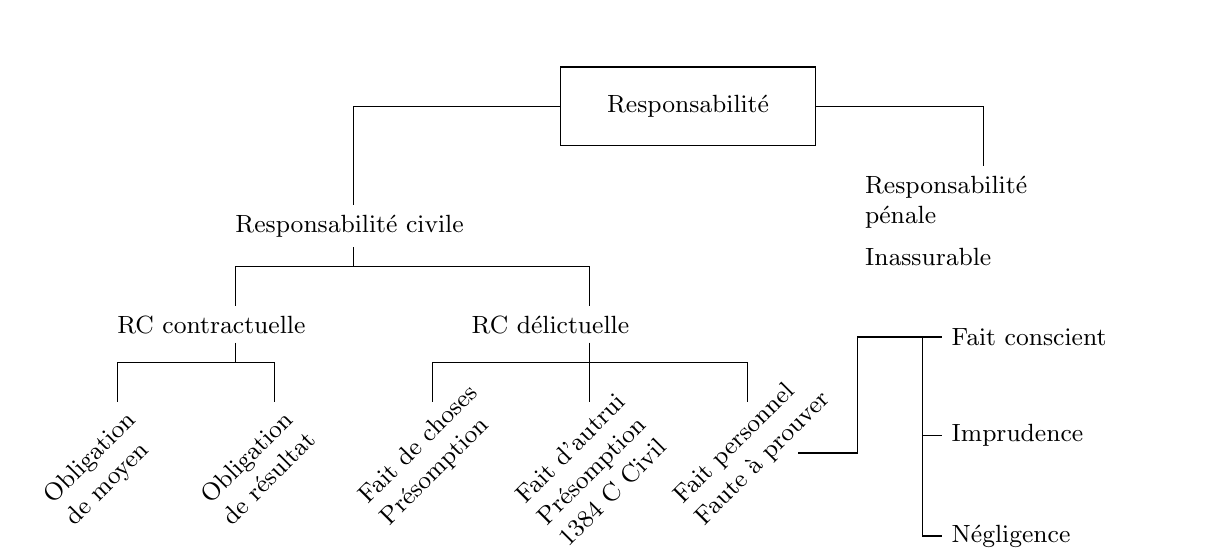
\begin{tikzpicture}[ every node/.style={font=\small,text width=3cm}, node distance=0.75cm and 1.cm]
			% Rectangle central "Responsabilit\'e"
			\node[draw, rectangle, minimum width=2cm, minimum height=1cm, align=center] (resp) at (0,0) {Responsabilit\'e};
			%		
			% Branches vers "Responsabilit\'e p\'enale" et "Responsabilit\'e civile"  +(-.25,0) |-
			\node[below right=of resp, xshift=-.5cm, yshift=.5cm] (penale) {Responsabilit\'e p\'enale};
			\node[below=0cm of penale] (inass) {Inassurable};
			\draw (resp.east) -| (penale.north);
			%		
			\node[below left=of resp] (civile) {Responsabilit\'e civile};
			\draw (resp.west) -| (civile.north);
			%		
			%		% Vers RC contractuelle et d\'elictuelle
			\node[below=of civile, xshift=-1.5cm] (rccontr) {RC contractuelle};
			\node[below=of civile, xshift=3cm] (rcdel) {RC d\'elictuelle};
			\draw (civile.south) |-  +(0,-0.25) -| (rccontr.north);
			\draw (civile.south) |-  +(0,-0.25) -| (rcdel.north);
			%		
			% Obligation de moyen / de r\'esultat
			\node[below= of rccontr, xshift=-1.5cm, rotate=45] (moyen) {Obligation\\ de moyen};
			\node[below= of rccontr, xshift=0.5cm, rotate=45] (resultat) {Obligation\\ de r\'esultat};
			\draw (rccontr.south) |-  +(0,-0.25) -| (moyen.north);
			\draw (rccontr.south) |-  +(0,-0.25) -| (resultat.north);
			%		
			% Sous RC d\'elictuelle : fait personnel / d'autrui / de choses
			\node[below=of rcdel, xshift=-2cm, rotate=45] (choses) {Fait de choses \\Pr\'esomption};
			\node[below= of rcdel, rotate=45] (autrui) {Fait d'autrui\\ Pr\'esomption \\ 1384 C Civil};
			\node[below= of rcdel, xshift=2cm, rotate=45] (personnel) {Fait personnel\\Faute \`a prouver};
			\draw (rcdel.south) |-  +(0,-0.25) -| (choses.north);
			\draw (rcdel.south) |-  +(0,-0.25) -| (autrui.north);
			\draw (rcdel.south) |-  +(0,-0.25) -| (personnel.north);
			%		
			% Faute \`a prouver et fait conscient sous fait personnel
			\node[right= of personnel, rotate=0, anchor=west] (fconscient) {Fait conscient};
			\draw (personnel.south) -|  +(0.75,0) |- (fconscient.west);
			%		
			% Imprudence / N\'eglience sous Fait conscient
			\node[below=of fconscient] (impru) {Imprudence};
			\node[below= of impru] (negl) {N\'egligence};
			\draw (fconscient.west)  |- +(-0.25,0) |- (impru.west);
			\draw (impru.west)  |- +(-0.25,0) |- (negl.west);
			% Source
			%		\node[below=2cm of moyen, anchor=west, text width=10cm] (source) {\small Source : Les Grands Principes de l'Assurance, Couilbault et Eliashberg, 10e \'edition};
		\end{tikzpicture}
	}
\end{center}

	
\end{f}


\begin{f}[Actuaire]
	
	En pratique, l'actuaire :
	\begin{itemize}[nosep]
		\item tarifie les produits d'assurance et de prévoyance, 
		\item estime les provisions techniques,
		\item projette les flux de trésorerie et valorise les engagements long terme,
		\item mesure le capital économique (SCR, ORSA) et contribue à l'ERM,
		\item conseille la direction sur la stratégie, la solvabilité et la conformité réglementaire.
	\end{itemize}
	
\end{f}
\end{multicols}

\newpage
\begin{center}
	\section*{Mathématiques Financières}
	\medskip
\end{center}


\begin{multicols}{2}
	
	% !TeX root = ActuarialFormSheet_MBFA-fr.tex
% !TeX spellcheck = fr_FR

\begin{f}[Capitalisation Actualisation]

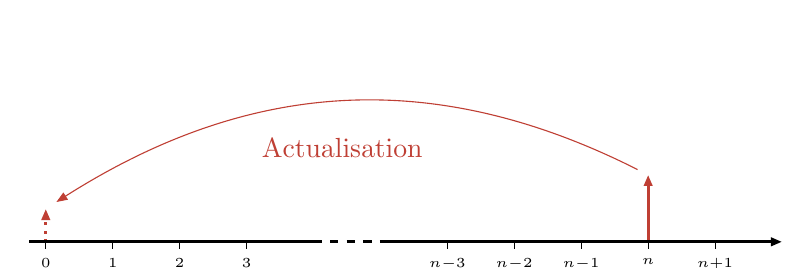
\begin{tikzpicture}[scale=0.85]
% Draw the x-axis and y-axis.
\def\w{11}
\def\n{9}
\draw[ line width=1,dotted, color=OrangeProfondIRA, arrows={-Stealth[length=4, inset=0]}] (0,0) -- (0,0.4909) node (A) {};	
\foreach \y in  {0,...,3} {
	\draw (\y,0) -- (\y,-0.1);
	\ifthenelse{\y>0 }{	\node[below] at (\y,-0.1) {\tiny $ \scriptstyle \y$};
		}{
		\node[below] at (\y,-0.1) {\tiny 0};}
}
\foreach \y in  {-3,...,1} {
	\draw (\y+\n,0) -- (\y+\n,-0.1);
	\ifthenelse{\y<0 }{\node[below] at (\y+\n,-0.1) {\tiny $\scriptstyle n \y$};}{}
	\ifthenelse{\y=0 }{\node[below] at (\y+\n,-0.1) {\tiny $\scriptstyle n $};
		\draw[ line width=1, color=OrangeProfondIRA, arrows={-Stealth[length=4, inset=0]}] (\y+\n,0) -- (\y+\n,1) node (B) {};}{}
	\ifthenelse{\y>0}{	\node[below] at (\y+\n,-0.1) {\tiny $\scriptstyle n+\y$};}{}
}
\draw[ line width=1] (-.25,0) -- (4,0);
\draw[ line width=1, dashed] (4,0) -- (5,0);
\draw[arrows={-Stealth[length=4, inset=0]}, line width=1] (5,0) -- (\w,0);
\draw[arrows={-Stealth[length=4, inset=0]},color=OrangeProfondIRA] (B)  to [bend right]  node [pos=0.5, below=10pt] {Actualisation}(A) ;
\end{tikzpicture}

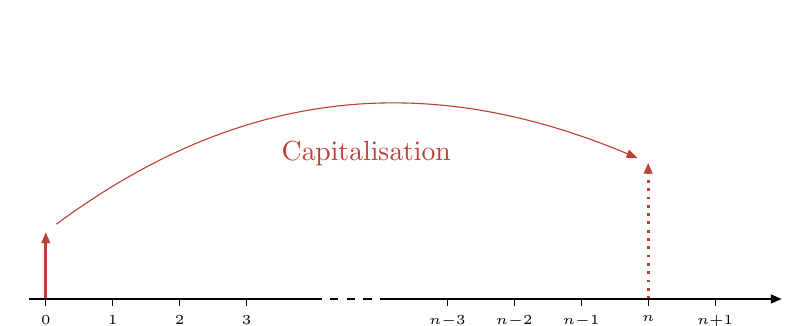
\begin{tikzpicture}[scale=0.85]
% Draw the x-axis and y-axis.
\def\w{11}
\def\n{9}
\draw[ line width=1, color=OrangeProfondIRA, arrows={-Stealth[length=4, inset=0]}] (0,0) -- (0,1) node (A) {};	
\foreach \y in  {0,...,3} {
	\draw (\y,0) -- (\y,-0.1);
	\ifthenelse{\y>0 }{	\node[below] at (\y,-0.1) {\tiny $ \scriptstyle \y$};
	}{
		\node[below] at (\y,-0.1) {\tiny 0};}
}
\foreach \y in  {-3,...,1} {
	\draw (\y+\n,0) -- (\y+\n,-0.1);
	\ifthenelse{\y<0 }{\node[below] at (\y+\n,-0.1) {\tiny $\scriptstyle n \y$};}{}
	\ifthenelse{\y=0 }{\node[below] at (\y+\n,-0.1) {\tiny $\scriptstyle n $};
		\draw[ line width=1,dotted, color=OrangeProfondIRA, arrows={-Stealth[length=4, inset=0]}] (\y+\n,0) -- (\y+\n,2.0368) node (B) {};}{}
	\ifthenelse{\y>0}{	\node[below] at (\y+\n,-0.1) {\tiny $\scriptstyle n+\y$};}{}
}
\draw[ line width=1] (-.25,0) -- (4,0);
\draw[ line width=1, dashed] (4,0) -- (5,0);
\draw[arrows={-Stealth[length=4, inset=0]}, line width=1] (5,0) -- (\w,0);
\draw[arrows={-Stealth[length=4, inset=0]},color=OrangeProfondIRA] (A)  to [bend left]  node [pos=0.55, below=10pt] {Capitalisation}(B) ;
\end{tikzpicture}

\end{f}
\hrule

\begin{f}[Les Intérêts]

\emph{Escompte ou taux précompté $d$}
     $$d=i/(1+i)$$
\emph{Intérêt simple $i$}
$$
I_t=P i t=P i \frac{k}{365}
$$
\emph{Intérêt composés $i$}
$$
V_n=P(1+i)^n=P\left(1+\frac{p}{100}\right)^n
$$
\emph{Intérêt continu $r$}
$$V_t=V_0\ e^{rt}$$

\emph{Taux effectif $i_e$}
$$
i_e=\left( 1+\frac{i}{m}\right) ^{m}-1
$$
où $i$ est le taux nominal et $m$ le nombre de périodes sur un an.

\emph{Taux équivalent $i^{(m)}$}
$$
i^{(m)}=m(1+i)^{1 / m}-1
$$

\emph{Taux nominal $i$ et taux périodique}

Le taux \textbf{nominal} ou taux \textbf{facial} permet de calculer les intérêts dus sur un an.
Le taux \textbf{périodique} correspond au taux nominal divisé par le nombre de périodes sur un an $i/m$.
Si le taux périodique est hebdomadaire, le taux nominal sera divisé par 52.
\end{f}
\hrule

\begin{f}[Valeur actuelle et valeur future]

La valeur actuelle (VA)  ou valeur présente (VP)  représente le capital qui doit être investi aujourd'hui à un taux d'intérêt composé annuel $i$ pour obtenir des flux de trésorerie futurs ($F_k$) aux moments $t_k$:
\begin{equation}
	VP = \sum_{k=1}^{n} F_k \times \frac{1}{(1+i)^{t_k}}
\label{ValeurActuelle}
\end{equation}
Lorsque les $F_k$ sont constants
\begin{equation}
	VP = K  \frac{1 - (1+i)^{-n}} {i}
\label{ValeurActuelleFluxCt}
\end{equation}

La valeur future (VF) représente la valeur du capital en $T$ qui, avec un taux d'intérêt composé annuel $i$,  capitalise les flux de trésorerie futurs ($F_k$) aux moments $t_k$.
\begin{equation}
	VF=V_n = \sum_{k=1}^{n} F_k \times (1+i)^{n-t_k}
\end{equation}
Plus généralement $VF= (1+i)^{n}VP$.
\end{f}
\hrule

\begin{f}[Annuités]
\ \newline


	Annuité certaine $a_{\lcroof{n}}$ (ou $a_{\lcroof{n}\;i}$ si le taux d'intérêt $i$ est utile à préciser) : c'est le cas par défaut en mathématiques financières. Ses paiements sont par exemple garantis par un contrat.
	
\begin{center}
	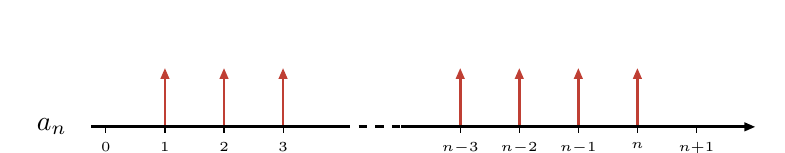
\begin{tikzpicture}[scale=0.75]
	% Draw the x-axis and y-axis.
	\def\w{11}
	\def\n{9}
	\node[left] at (-.5,0) {$a_{\lcroof{n}}$};
	\foreach \y in  {0,...,3} {
	\draw (\y,0) -- (\y,-0.1);
	\ifthenelse{\y>0 }{	\node[below] at (\y,-0.1) {\tiny $ \scriptstyle \y$};
		\draw[ line width=1, color=OrangeProfondIRA, arrows={-Stealth[length=4, inset=0]}] (\y,0) -- (\y,1);}{
		\node[below] at (\y,-0.1) {\tiny 0};}
}
\foreach \y in  {-3,...,1} {
	\draw (\y+\n,0) -- (\y+\n,-0.1);
	\ifthenelse{\y<0 }{\node[below] at (\y+\n,-0.1) {\tiny $\scriptstyle n \y$};}{}
	\ifthenelse{\y=0 }{\node[below] at (\y+\n,-0.1) {\tiny $\scriptstyle n $};}{}
	\ifthenelse{\y>0}{	\node[below] at (\y+\n,-0.1) {\tiny $\scriptstyle n+\y$};}{}
	\ifthenelse{\y<1 }{	\draw[ line width=1, color=OrangeProfondIRA, arrows={-Stealth[length=4, inset=0]}] (\y+\n,0) -- (\y+\n,1);}
}
\draw[ line width=1] (-.25,0) -- (4,0);
\draw[ line width=1, dashed] (4,0) -- (5,0);
\draw[arrows={-Stealth[length=4, inset=0]}, line width=1] (5,0) -- (\w,0);
\end{tikzpicture}
\end{center}
$$
\ddot{a}_{\lcroof{n}}=1+v+\cdots+v^{n-1}=\frac{1-v^{n}}{1-v}=\frac{1-v^{n}}{d}
$$


Annuité contingente $\ddot{a}_{x}$: ses paiements sont conditionnés à un événement  aléatoire, comme lors d'une rente viagère d'un individu d'âge $x$. Dans cet exemple, ils courent jusqu'à ce que mort s'ensuive :

\begin{center}
	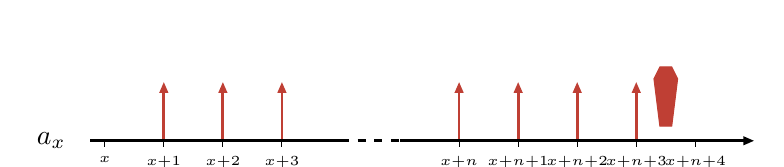
\begin{tikzpicture}[scale=0.75]
	% Draw the x-axis and y-axis.
	\def\w{11}
	\def\n{6}
	\node[left] at (-.5,0) {$a_{x}$};
	
	\begin{scope}[shift={(\n+.5+3,.25)}]
		\draw[color=OrangeProfondIRA,scale=0.2,fill=OrangeProfondIRA] \Cerceuil;
	\end{scope}
	\foreach \y in  {0,...,3} {
		\draw (\y,0) -- (\y,-0.1);
		\ifthenelse{\y>0 }{	\node[below] at (\y,-0.1) {\tiny $ \scriptstyle x+\y$};
			\draw[ line width=1, color=OrangeProfondIRA, arrows={-Stealth[length=4, inset=0]}] (\y,0) -- (\y,1);}{
			\node[below] at (\y,-0.1) {\tiny $ \scriptstyle x$};}
	}
	\foreach \y in  {0,...,4} {
		\draw (\y+\n,0) -- (\y+\n,-0.1);
		\ifthenelse{\y>0 }{\node[below] at (\y+\n,-0.1) {\tiny $\scriptstyle x+n+\y$};}{
			\node[below] at (\y+\n,-0.1) {\tiny $\scriptstyle x+n$};}
		\ifthenelse{\y<4 }{	\draw[ line width=1, color=OrangeProfondIRA, arrows={-Stealth[length=4, inset=0]}] (\y+\n,0) -- (\y+\n,1);}
	}
\draw[ line width=1] (-.25,0) -- (4,0);
\draw[ line width=1, dashed] (4,0) -- (5,0);
\draw[arrows={-Stealth[length=4, inset=0]}, line width=1] (5,0) -- (\w,0);
\end{tikzpicture}	

\end{center}
La date du décès est représenté ici par un petit cercueil. Cette forme d'annuité sera largement étudiée dans la partie actuariat vie.
Annuité à terme échu (\engl{immédiate}) $a_{\lcroof{n}}$ : ses paiements périodiques sont effectués à la fin de chaque période de paiement, comme pour le salaire payé en fin de mois. C'est le cas par défaut, illustré précédemment pour l'annuité certaine.
$$
\ddot{a}_{\lcroof{n}}=1+v+\cdots+v^{n-1}=\frac{1-v^{n}}{1-v}=\frac{1-v^{n}}{d}
$$
%
$$
	\mathrm{PV}_{\lcroof{n}}^{\text {due }}=K \ddot{a}_{\lcroof{n}}=K \frac{1-v^{n}}{d} 
$$

Annuité à terme à échoir (\engl{due}) $\ddot{a}_{\lcroof{n}}$:  ses paiements périodiques sont effectués au début de chaque période de paiement, comme pour un loyer par exemple.

\begin{center}
	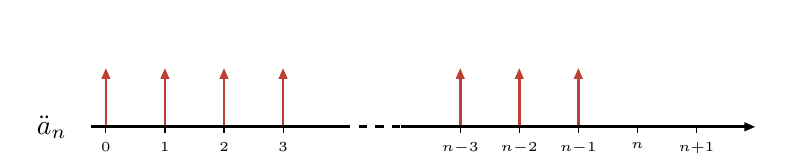
\begin{tikzpicture}[scale=0.75]
		% Draw the x-axis and y-axis.
		\def\w{11}
		\def\n{9}
		\node[left] at (-.5,0) {$\ddot{a}_{\lcroof{n}}$};
		\foreach \y in  {0,...,3} {
			\draw (\y,0) -- (\y,-0.1);
				\node[below] at (\y,-0.1) {\tiny $ \scriptstyle \y$};
				\draw[ line width=1, color=OrangeProfondIRA, arrows={-Stealth[length=4, inset=0]}] (\y,0) -- (\y,1);
		}
		\foreach \y in  {-3,...,1} {
			\draw (\y+\n,0) -- (\y+\n,-0.1);
			\ifthenelse{\y<0 }{\node[below] at (\y+\n,-0.1) {\tiny $\scriptstyle n \y$};}{}
			\ifthenelse{\y=0 }{\node[below] at (\y+\n,-0.1) {\tiny $\scriptstyle n $};}{}
			\ifthenelse{\y>0}{	\node[below] at (\y+\n,-0.1) {\tiny $\scriptstyle n+\y$};}{}
			\ifthenelse{\y<0 }{	\draw[ line width=1, color=OrangeProfondIRA, arrows={-Stealth[length=4, inset=0]}] (\y+\n,0) -- (\y+\n,1);}{}
		}
		\draw[ line width=1] (-.25,0) -- (4,0);
		\draw[ line width=1, dashed] (4,0) -- (5,0);
		\draw[arrows={-Stealth[length=4, inset=0]}, line width=1] (5,0) -- (\w,0);
	\end{tikzpicture}
\end{center}
aussi notée $\mathrm{PV}^{\mathrm{im}}$ :
$$
a_{\lcroof{n}}=v+v^{2}+\cdots+v^{n}=\frac{1-v^{n}}{i}=v \frac{1-v^{n}}{1-v}
$$
%
$$
	\mathrm{PV}_{\lcroof{n}}^{\mathrm{im}}=K a_{\lcroof{n}}=K \frac{1-v^{n}}{i} 
$$
Annuité  perpétuelle $a$ ou  $a_{\lcroof{n\infty}}$: 
$$
a=1/i
$$
Annuité différée $_{m|}a_{\lcroof{n}}$: ses paiements ne commencent pas dans la première période mais après $m$ périodes, $m$ étant fixé à l'avance. 
\begin{center}
	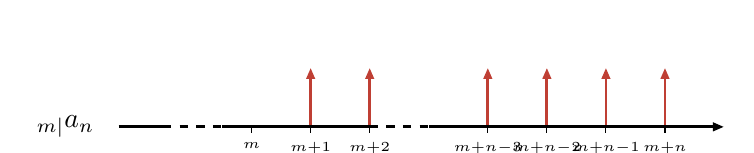
\begin{tikzpicture}[scale=0.75]
		% Draw the x-axis and y-axis.
\def\w{10}
\def\n{9}
\def\m{2}
\node[left] at (-.5,0) {$_{m|}a_{\lcroof{n}}$};
\foreach \y in  {0,...,2} {
	\draw (\y+\m,0) -- (\y+\m,-0.1);
	\ifthenelse{\y<0 }{\node[below] at (\y+\m,-0.1) {\tiny $\scriptstyle m \y$};}{}
\ifthenelse{\y=0 }{\node[below] at (\y+\m,-0.1) {\tiny $\scriptstyle m $};}{}
\ifthenelse{\y>0}{	\node[below] at (\y+\m,-0.1) {\tiny $\scriptstyle m+\y$};
		\draw[ line width=1, color=OrangeProfondIRA, arrows={-Stealth[length=4, inset=0]}] (\y+\m,0) -- (\y+\m,1);
		}
}
\foreach \y in  {-3,...,0} {
	\draw (\y+\n,0) -- (\y+\n,-0.1);
	\ifthenelse{\y<0 }{\node[below] at (\y+\n,-0.1) {\tiny $\scriptstyle m+n \y$};}{}
	\ifthenelse{\y=0 }{\node[below] at (\y+\n,-0.1) {\tiny $\scriptstyle m+n $};}{}
	\ifthenelse{\y>0}{	\node[below] at (\y+\n,-0.1) {\tiny $\scriptstyle m+n+\y$};}{}
	\ifthenelse{\y<1 }{	\draw[ line width=1, color=OrangeProfondIRA, arrows={-Stealth[length=4, inset=0]}] (\y+\n,0) -- (\y+\n,1);}
}
\draw[ line width=1] (-.25,0) -- (0.5,0);
\draw[ line width=1, dashed] (0.5,0) -- (1.5,0);
\draw[ line width=1] (1.5,0) -- (4,0);
\draw[ line width=1, dashed] (4,0) -- (5,0);
		\draw[arrows={-Stealth[length=4, inset=0]}, line width=1] (5,0) -- (\w,0);
	\end{tikzpicture}	
	
\end{center}


Annuité périodique / mensuelle $a^{(m)}$ : la périodicité par défaut est un an, mais le paiement  unitaire peut être aussi réparti sur $m$ périodes dans l'année.

\begin{center}
	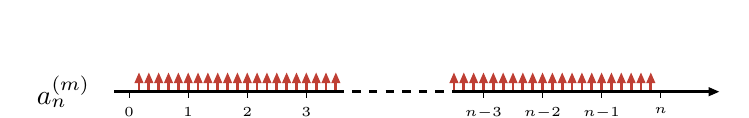
\begin{tikzpicture}[scale=0.75]
		% Draw the x-axis and y-axis.
		\def\w{10}
		\def\n{9}
		\def\m{6}
		\node[left] at (-.5,0) {$a_{\lcroof{n}}^{(m)}$};
		\foreach \y in  {0,...,3} {
			\draw (\y,0) -- (\y,-0.1);
			\ifthenelse{\y>0 }{	\node[below] at (\y,-0.1) {\tiny $ \scriptstyle \y$};}{
				\node[below] at (\y,-0.1) {\tiny 0};}
		}
		\pgfmathparse{3.5*\m} 
		\foreach \y in  {1,...,\pgfmathresult} {
			\ifthenelse{\y>0 }{	
				\draw[ line width=1, color=OrangeProfondIRA, arrows={-Stealth[length=4, inset=0]}] (\y/\m,0) -- (\y/\m,2/\m);}{}
		}
		\foreach \y in  {-3,...,0} {
			\draw (\y+\n,0) -- (\y+\n,-0.1);
			\ifthenelse{\y<0 }{\node[below] at (\y+\n,-0.1) {\tiny $\scriptstyle n \y$};}{}
			\ifthenelse{\y=0 }{\node[below] at (\y+\n,-0.1) {\tiny $\scriptstyle n $};}{}
			\ifthenelse{\y>0}{	\node[below] at (\y+\n,-0.1) {\tiny $\scriptstyle n+\y$};}{}
		}
		\pgfmathparse{3.5*\m} 
		\foreach \y  in  {1,...,\pgfmathresult} {
		\draw[ line width=1, color=OrangeProfondIRA, arrows={-Stealth[length=4, inset=0]}] (-\y/\m+\n,0) -- (-\y/\m+\n,2/\m);
		}
		\draw[ line width=1] (-.25,0) -- (3.5,0);
		\draw[ line width=1, dashed] (3.5,0) -- (5.5,0);
		\draw[arrows={-Stealth[length=4, inset=0]}, line width=1] (5.5,0) -- (\w,0);
	\end{tikzpicture}
\end{center}

 Si    $i^{(m)}$ représente le taux d'intérêt (annuel) nominal équivalent avec $m$ période annuelle $i^{(m)}= m\left((1+i)^{1 / m}-1\right)$ .

De même $d^{(m)} $ taux d'escompte nominal conforme à $i$ et $m$ : $d^{(m)}= m\left(1-(1-d)^{1 / m}\right)$.

$$
\ddot{a}_{\lcroof{n}}^{(m)}=\frac{1}{m} \sum_{k=0}^{m n-1} v^{\frac{k}{m}}=\frac{d}{d^{(m)}} \ddot{a}_{\lcroof{n}}=\frac{1-v^{n}}{d^{(m)}} \approx \ddot{a}_{\lcroof{n}}+\frac{m-1}{2 m}\left(1-v^{n}\right)
$$
$$
a_{\lcroof{n}}^{(m)}=\frac{1}{m} \sum_{k=1}^{m n} v^{\frac{k}{m}}=\frac{i}{i^{(m)}} a_{\lcroof{n}}=\frac{1-v^{n}}{i^{(m)}} \approx a_{\lcroof{n}}-\frac{m-1}{2 m}\left(1-v^{n}\right)
$$
Annuité unitaire $a$ : elle est utilisée lors de la construction de formules d'annuité.
Pour une annuité constante, le montant total versé chaque année est de~1, quelque soit $m$.  

Annuité dynamique, croissante/décroissante $Ia$/$Da$ : dans sa forme la plus simple, elle verse un montant qui démarre à 1 ($n$) et qui croit (décroit) à chaque période de façon arithmétique ou géométrique. Dans l'exemple suivant, la progression est arithmétique.
On utilise le préfixe $I$ (\engl{increasing}) pour indiquer les annuités croissantes et $D$ (\engl{decreasing}) pour les annuités dégressives.
	
\begin{center}
	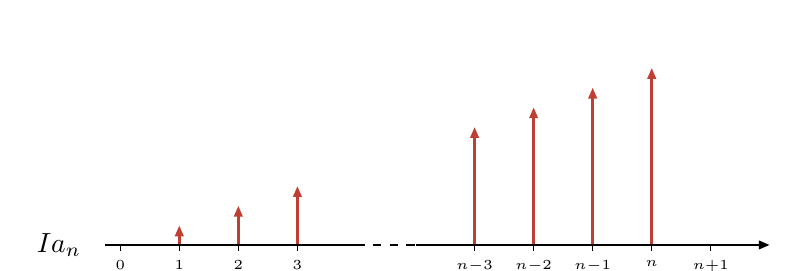
\begin{tikzpicture}[scale=0.75]
		% Draw the x-axis and y-axis.
		\def\w{11}
		\def\n{9}
		\node[left] at (-.5,0) {$Ia_{\lcroof{n}}$};
		\foreach \y in  {0,...,3} {
			\draw (\y,0) -- (\y,-0.1);
			\ifthenelse{\y>0 }{	\node[below] at (\y,-0.1) {\tiny $ \scriptstyle \y$};
				\draw[ line width=1, color=OrangeProfondIRA, arrows={-Stealth[length=4, inset=0]}] (\y,0) -- (\y,\y/3);}{
				\node[below] at (\y,-0.1) {\tiny 0};}
		}
		\foreach \y in  {-3,...,1} {
			\draw (\y+\n,0) -- (\y+\n,-0.1);
			\ifthenelse{\y<0 }{\node[below] at (\y+\n,-0.1) {\tiny $\scriptstyle n \y$};}{}
			\ifthenelse{\y=0 }{\node[below] at (\y+\n,-0.1) {\tiny $\scriptstyle n $};}{}
			\ifthenelse{\y>0}{	\node[below] at (\y+\n,-0.1) {\tiny $\scriptstyle n+\y$};}{}
			\ifthenelse{\y<1 }{	\draw[ line width=1, color=OrangeProfondIRA, arrows={-Stealth[length=4, inset=0]}] (\y+\n,0) -- (\y+\n,\y/3+\n/3);}
		}
		\draw[ line width=1] (-.25,0) -- (4,0);
		\draw[ line width=1, dashed] (4,0) -- (5,0);
		\draw[arrows={-Stealth[length=4, inset=0]}, line width=1] (5,0) -- (\w,0);
	\end{tikzpicture}
	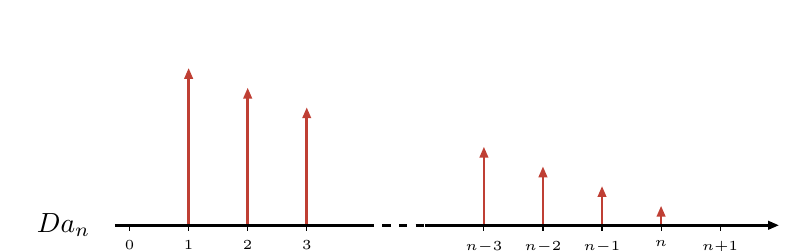
\begin{tikzpicture}[scale=0.75]
	% Draw the x-axis and y-axis.
	\def\w{11}
	\def\n{9}
	\node[left] at (-.5,0) {$Da_{\lcroof{n}}$};
	\foreach \y in  {0,...,3} {
		\draw (\y,0) -- (\y,-0.1);
		\ifthenelse{\y>0 }{	\node[below] at (\y,-0.1) {\tiny $ \scriptstyle \y$};
			\draw[ line width=1, color=OrangeProfondIRA, arrows={-Stealth[length=4, inset=0]}] (\y,0) -- (\y,\n/3-\y/3);}{
			\node[below] at (\y,-0.1) {\tiny 0};}
	}
	\foreach \y in  {-3,...,1} {
		\draw (\y+\n,0) -- (\y+\n,-0.1);
		\ifthenelse{\y<0 }{\node[below] at (\y+\n,-0.1) {\tiny $\scriptstyle n \y$};}{}
		\ifthenelse{\y=0 }{\node[below] at (\y+\n,-0.1) {\tiny $\scriptstyle n $};}{}
		\ifthenelse{\y>0}{	\node[below] at (\y+\n,-0.1) {\tiny $\scriptstyle n+\y$};}{}
		\ifthenelse{\y<1 }{	\draw[ line width=1, color=OrangeProfondIRA, arrows={-Stealth[length=4, inset=0]}] (\y+\n,0) -- (\y+\n,1/3-\y/3);}
	}
	\draw[ line width=1] (-.25,0) -- (4,0);
	\draw[ line width=1, dashed] (4,0) -- (5,0);
	\draw[arrows={-Stealth[length=4, inset=0]}, line width=1] (5,0) -- (\w,0);
\end{tikzpicture}
\end{center}

\begin{equation}
(I \ddot{a})_{\lcroof{n}}=1+2 v+\cdots+n v^{n-1}=\frac{1}{d}\left(\ddot{a}_{\lcroof{n}}-n v^{n}\right)
\label{Ian}
\end{equation}
avec, on le rappelle,  $d=i/(1+i)$ et à terme échu (\engl{immediate})
$$
(I a)_{\lcroof{n}}=v+2 v^{2}+\cdots+n v^{n}=\frac{1}{i}\left(\ddot{a}_{\lcroof{n}}-n v^{n}\right)
$$
$$
(D \ddot{a})_{\lcroof{n}}=n+(n-1) v+\cdots+v^{n-1}=\frac{1}{d}\left(n-a_{\lcroof{n}}\right)
$$
et à terme échu :
$$
(D a)_{\lcroof{n}}=n v+(n-1) v^{2}+\cdots+v^{n}=\frac{1}{i}\left(n-a_{\lcroof{n}}\right)
$$




\end{f}
\hrule

\begin{f}[L'emprunt (Indivis)]
\ \newline

La principale propriété de l'emprunt est de considéré séparément les intérêts du remboursement (ou de l'amortissement).

Par un remboursement constant ou par annuité constante: la somme de l'amortissement et de l'intérêt à chaque période est constante. 

\begin{center}
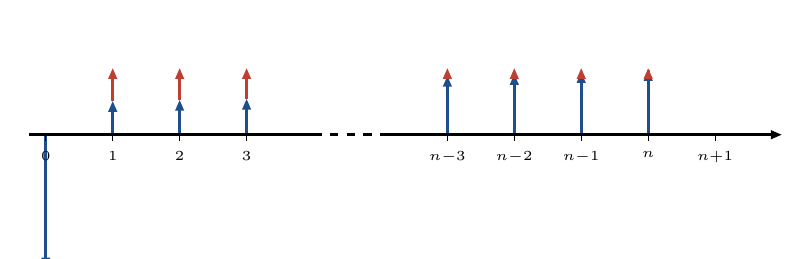
\begin{tikzpicture}[scale=0.85]
% Draw the x-axis and y-axis.
\def\w{11}
\def\n{9}
\def\duree{23}
\def\a{16.713332269}
\def\v{1.031415^(-1)} 
\draw[ line width=1, color=BleuProfondIRA, arrows={-Stealth[length=4, inset=0]}] (0,0) -- (0,-2);
\foreach \y in  {0,...,3} {
	\draw (\y,0) -- (\y,-0.1);
	\ifthenelse{\y>0 }{	\node[below] at (\y,-0.1) {\tiny $ \scriptstyle \y$};
	\pgfmathpow{\v}{\duree-\y} 	
	\let\Interet\pgfmathresult
		\draw[ line width=1, color=BleuProfondIRA, arrows={-Stealth[length=4, inset=0]}] (\y,0) -- (\y,\Interet);
		\draw[ line width=1, color=OrangeProfondIRA, arrows={-Stealth[length=4, inset=0]}] (\y,\Interet) -- (\y,1);}{
		\node[below] at (\y,-0.1) {\tiny 0};}
}
\foreach \y in  {-3,...,1} {
	\pgfmathpow{\v}{-\y+1} 	
	\let\Interet\pgfmathresult
	\draw (\y+\n,0) -- (\y+\n,-0.1);
	\ifthenelse{\y<0 }{\node[below] at (\y+\n,-0.1) {\tiny $\scriptstyle n \y$};}{}
	\ifthenelse{\y=0 }{\node[below] at (\y+\n,-0.1) {\tiny $\scriptstyle n $};}{}
	\ifthenelse{\y>0}{	\node[below] at (\y+\n,-0.1) {\tiny $\scriptstyle n+\y$};}{}
	\ifthenelse{\y<1 }{	
		\draw[ line width=1, color=BleuProfondIRA, arrows={-Stealth[length=4, inset=0]}] (\y+\n,0) -- (\y+\n,\Interet);
		\draw[ line width=1, color=OrangeProfondIRA, arrows={-Stealth[length=4, inset=0]}] (\y+\n,\Interet) -- (\y+\n,1);}
}
\draw[ line width=1] (-.25,0) -- (4,0);
\draw[ line width=1, dashed] (4,0) -- (5,0);
\draw[arrows={-Stealth[length=4, inset=0]}, line width=1] (5,0) -- (\w,0);
\end{tikzpicture}
\end{center}
	
    
    Par un amortissement constant.
\begin{center}
\begin{tikzpicture}[scale=0.85]
% Draw the x-axis and y-axis.
\def\w{11}
\def\n{9}
\def\duree{23}
\def\i{0.031415}
\draw[ line width=1, color=BleuProfondIRA, arrows={-Stealth[length=4, inset=0]}] (0,0) -- (0,-2);
\foreach \y in  {0,...,3} {
\draw (\y,0) -- (\y,-0.1);
\ifthenelse{\y>0 }{	\node[below] at (\y,-0.1) {\tiny $ \scriptstyle \y$};
	\pgfmathparse{(\duree-\y)*\i} 	
	\let\Interet\pgfmathresult
	\draw[ line width=1, color=BleuProfondIRA, arrows={-Stealth[length=4, inset=0]}] (\y,0) -- (\y,1);
	\draw[ line width=1, color=OrangeProfondIRA, arrows={-Stealth[length=4, inset=0]}] (\y,1) -- (\y,1+\Interet);}{
	\node[below] at (\y,-0.1) {\tiny 0};}
}
\foreach \y in  {-3,...,1} {
	\pgfmathparse{(-\y+1)*\i} 	
\let\Interet\pgfmathresult
\draw (\y+\n,0) -- (\y+\n,-0.1);
\ifthenelse{\y<0 }{\node[below] at (\y+\n,-0.1) {\tiny $\scriptstyle n \y$};}{}
\ifthenelse{\y=0 }{\node[below] at (\y+\n,-0.1) {\tiny $\scriptstyle n $};}{}
\ifthenelse{\y>0}{	\node[below] at (\y+\n,-0.1) {\tiny $\scriptstyle n+\y$};}{}
\ifthenelse{\y<1 }{	
	\draw[ line width=1, color=BleuProfondIRA, arrows={-Stealth[length=4, inset=0]}] (\y+\n,0) -- (\y+\n,1);
\draw[ line width=1, color=OrangeProfondIRA, arrows={-Stealth[length=4, inset=0]}] (\y+\n,1) -- (\y+\n,1+\Interet);}{}
}
\draw[ line width=1] (-.25,0) -- (4,0);
\draw[ line width=1, dashed] (4,0) -- (5,0);
\draw[arrows={-Stealth[length=4, inset=0]}, line width=1] (5,0) -- (\w,0);
\end{tikzpicture}
\end{center}

    
Par un remboursement in fine, où l'intérêt est constant. Seuls les intérêts sont versés périodiquement jusqu'au terme, moment où le remboursement total est effectué.
	
\begin{center}
\begin{tikzpicture}[scale=0.85]
% Draw the x-axis and y-axis.
\def\w{11}
\def\n{9}
\def\duree{23}
\def\i{3*0.031415}
\draw[ line width=1, color=BleuProfondIRA, arrows={-Stealth[length=4, inset=0]}] (0,0) -- (0,-2);
\foreach \y in  {0,...,3} {
	\draw (\y,0) -- (\y,-0.1);
	\ifthenelse{\y>0 }{	\node[below] at (\y,-0.1) {\tiny $ \scriptstyle \y$};
%				\draw[ line width=1, color=BleuProfondIRA, arrows={-Stealth[length=4, inset=0]}] (\y,0) -- (\y,1);
		\draw[ line width=1, color=OrangeProfondIRA, arrows={-Stealth[length=4, inset=0]}] (\y,0) -- (\y,2*\i);}{
		\node[below] at (\y,-0.1) {\tiny 0};}
}
\foreach \y in  {-3,...,1} {
	\draw (\y+\n,0) -- (\y+\n,-0.1);
	\ifthenelse{\y<0 }{\node[below] at (\y+\n,-0.1) {\tiny $\scriptstyle n \y$};
		\draw[ line width=1, color=OrangeProfondIRA, arrows={-Stealth[length=4, inset=0]}] (\y+\n,0) -- (\y+\n,2*\i);}{}
	\ifthenelse{\y=0 }{
		\draw[ line width=1, color=BleuProfondIRA, arrows={-Stealth[length=4, inset=0]}] (\y+\n,0) -- (\y+\n,2);
		\draw[ line width=1, color=OrangeProfondIRA, arrows={-Stealth[length=4, inset=0]}] (\y+\n,2) -- (\y+\n,2+2*\i);
		\node[below] at (\y+\n,-0.1) {\tiny $\scriptstyle n $};}{}
	\ifthenelse{\y>0}{	\node[below] at (\y+\n,-0.1) {\tiny $\scriptstyle n+\y$};}{}
}
\draw[ line width=1] (-.25,0) -- (4,0);
\draw[ line width=1, dashed] (4,0) -- (5,0);
\draw[arrows={-Stealth[length=4, inset=0]}, line width=1] (5,0) -- (\w,0);
\end{tikzpicture}
\end{center}

\end{f}
\hrule \

\begin{f} [Tableau d'amortissement de l'emprunt]
\ \newline

	\footnotesize
\renewcommand{\arraystretch}{2}
\begin{tabular}{|m{10ex}|m{19ex}|m{19ex}|m{17ex}|}
\rowcolor{BleuProfondIRA!40}   	\hline &\textbf{ In fine}			&   	\textbf{	Amortissements  constants} &  		\textbf{Annuités  constantes} \\
	\hline Capital restant dû $S_k$ & $T_k=S_0$, $T_n=0$& $S_{0}\left(1-\frac{k}{n}\right)$ & $S_{0} \frac{1-v^{n-k}}{1-v^{n}}$\\
	\hline Intérêts $U_k$ 		& $i\times S_0$ & $S_{0}\left(1-\frac{k-1}{n}\right) i$ & $K\left(1-v^{n-k+1}\right)$ \\
	\hline Amortis\-sements $T_k$ &	$T_k=O$, $T_n=S_0$ & $\frac{S_{0}}{n}$ & $K v^{n-k+1}$ \\
	\hline Annuité $K_k$ & 	$K_k=i S_0$, $K_n=(1+i)S_0$ 	 & $\frac{S_{0}}{n}(1-(n-k+1) i) $ & $K=S_{0} \frac{i}{1-v^{n}} $ \\
%	\hline Coût de l'emprunt & $1 \times K \times N$ & $1 \times K \times \frac{N+1}{2}$ & $K\left(\frac{N i}{1-(1+i)^{-N}}-1\right)$ \\
	\hline
\end{tabular}

\end{f}

\end{multicols}

\begin{center}
\section*{Finances de Marchés}
    \medskip
\end{center}

\begin{multicols}{2}

% !TeX root = ActuarialFormSheet_MBFA-fr.tex
% !TeX spellcheck = fr_FR
\def\scaleBS{.95}

\begin{f}[Fonctionnement des marchés]
	
La \textbf{Bourse} (\engl{Exchange}) - lieu d'échange - permet, de fait, la rencontre physique entre les demandeurs et offreurs de capitaux.
Les principales cotations concernent les \textbf{actions} (\engl{equities}), les \textbf{obligations} (\engl{Fixed Income}) et les \textbf{matières premières} (\engl{commodities}).
Sont cotés des \textbf{titres} comme des actions ou des obligations, des \textbf{fonds} (\engl{Exhange Trade Funds} qui répliquent des indices actions, ETC ou ETN qui répliquent des indices plus spécifiques ou des matières premières, SICAV ou FCP, bons de souscription, \engl{warrant}), des \textbf{contrats à terme},  des \textbf{options}, des \textbf{swaps} ou encore des \textbf{produits structurés}.

L'\textbf{Autorité des marchés financiers} (\href{https://www.amf-france.org/fr}{AMF})  veille :
\begin{itemize}
	\item à la protection de l'épargne investie; 
	\item à l'information des investisseurs ; 
	\item au bon fonctionnement des marchés. 
\end{itemize}

\textbf{\href{https://www.euronext.com/fr}{Euronext}} (dont
\href{https://www.euronext.com/en/markets/amsterdam}{Amsterdam}, 
\href{https://www.euronext.com/en/markets/brussels}{Brussels}, 
\href{https://www.euronext.com/en/markets/lisbon}{Lisbon}, 
et \href{https://www.euronext.com/en/markets/paris}{Paris}) est la principale bourse en France. 
%
Ses concurrents sont entre autres \textbf{\href{https://www.deutsche-boerse.com/dbg-en/}{Deutsche Börse}} 
(dont \href{https://www.eurex.com/}{Eurex}, 
\href{https://www.eex.com/en/}{eex}) en Europe, 
%
ou \textbf{\href{https://www.ice.com/}{ICE}} (dont
\href{https://www.nyse.com/index}{NYSE (2012)}, 
\href{https://www.ice.com/about/history}{NYBOT (2005)}, 
\href{https://www.ice.com/futures-europe}{IPE (2001), LIFFE}) 
%
et \textbf{\href{https://www.cmegroup.com/}{CME Group}} (y compris
\href{https://www.cmegroup.com/company/cbot.html}{CBOT}, 
\href{https://www.cmegroup.com/company/nymex.html}{NYMEX}, 
\href{https://www.cmegroup.com/company/comex.html}{COMEX}) aux États-Unis.

Le \textbf{marché de gré à gré} (\textbf{OTC}, \textit{Over-The-Counter}) représente une part majeure des volumes échangés hors marchés organisés.
Depuis le G20 de Pittsburgh (2009), certains dérivés OTC standardisés doivent être compensés via une entité centrale.
Ces \textbf{CCP} (\textit{Central Counterparties}) jouent ainsi le rôle de \textbf{chambre de compensation} (\textit{clearing}) : elles remplacent le contrat bilatéral par deux contrats entre chaque partie et la CCP.

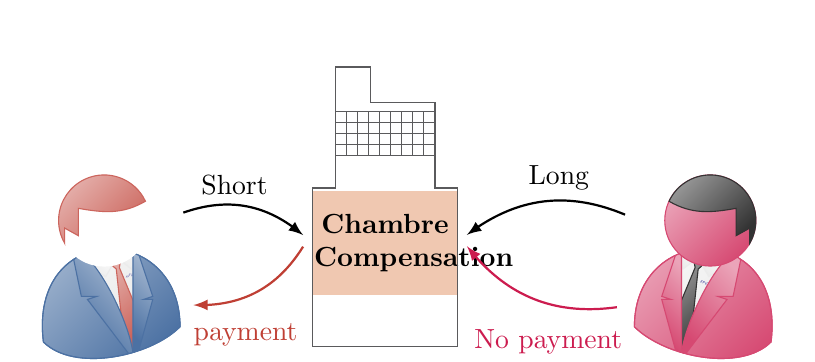
\begin{tikzpicture}[scale=.47]
	\node[businessman,minimum size=1.75cm,monogramtext=MPG,tie=OrangeProfondIRA, shirt=BleuProfondIRA,skin=white,hair=OrangeProfondIRA] at (-8,0) (MPG){Short position};
	\node[businessman,mirrored,minimum size=1.75cm,monogramtext=SPG,shirt=FushiaIRA, tie=black,skin=FushiaIRA, hair=black] at (8,0) (SPG){Long position};
	%  	
	\begin{scope}[yscale=-0.03, xscale=0.03, shift={(-150,-200)}]
		%  		
		%Usine
		\draw [OrangeMoyenIRA!40,fill] (65,132) rectangle (195,225)  node [pos=0.5,text width=1.8cm, align=center] {\color{black}\bfseries Chambre Compensation} ;
		%Straight Lines [id:da13081779728777443] 
		%	\draw (65,272) -- (474,272) -- (474,320);
		%Shape: Polygon [id:ds025531371089408395] 
		\draw   [GrisLogoIRA] (195,272) -- (65,272) -- (65,129) -- (85,129) -- (85,20) -- (117,20)  -- (117,52)-- (175,52) -- (175,129) -- (195,129) -- cycle ;
		%Shape: Grid [id:dp09099790819019526] 
		%	\draw  [draw opacity=0] (117,129) -- (195,129) -- (195,169) -- (117,169) -- cycle ; 
		\draw  [GrisLogoIRA] (95,100) -- (95,60)(105,100) -- (105,60)(115,100) -- (115,60)(125,100) -- (125,60)(135,100) -- (135,60)(145,100) -- (145,60)(155,100) -- (155,60)(165,100) -- (165,60) ; 
		\draw  [GrisLogoIRA]  (85,100) -- (175,100)(85,90) -- (175,90)(85,80) -- (175,80)(85,70) -- (175,70)(85,60) -- (175,60) ; 
		%
		\draw  (65,175) node (a) {} ;
		\draw  (195,175) node (b) {} ;
		%Shape: Rectangle [id:dp30583722611654374] 
	\end{scope}
	% 	
	\draw[->,>=latex, thick] (MPG) to [bend left]  node[pos=0.4, above]{Short} (a);
	\draw[<-,>=latex, thick,OrangeProfondIRA] (MPG) to [bend right]  node[pos=0.4, below=.2]{payment} (a);
	\draw[->,>=latex, thick,FushiaIRA] (SPG) to [bend left] node[pos=0.4, below=.2]{No payment}  (b);
	\draw[->,>=latex, thick] (SPG) to [bend right] node[pos=0.4, above]{Long} (b);
	%  	
\end{tikzpicture}
\medskip

\end{f}
\hrule

\begin{f}[Le Marché Monétaire]
Les titres de taux à court terme, négociés sur les marchés monétaires, sont généralement à \textbf{intérêts précomptés}. 
Les taux nominaux sont alors annuels et les calculs utilisent les \textbf{taux proportionnels} pour s'adapter aux durées inférieures à un an.
Ces titres sont cotés ou évalués selon le principe de l'escompte et avec  une convention de calendrier Euro-30/360.

Sur le marché américain, les titres de dette publique sont appelés :
 Bons du Trésor ({T-bills}) : ZC < 1 an,  Obligations du Trésor ({T-notes}) : ZC < 10 ans,
Obligations du Trésor ({T-bonds}) : obligations à coupon avec une maturité > 10 ans.


Ce sont principalement :
\begin{itemize}
  \item \textbf{BTF (bons du Trésor à taux fixe, France) :} émis à 13, 26, 52 sem., taux précompté, adjudication hebdo, nominal 1~€, règlement à J+2.
  
  \item \textbf{Bons du Trésor > 1 an :} mêmes règles que les obligations (voir section suivante).
  
  \item \textbf{Certificats de dépôt (CDN) :} titres émis par banques émis à taux fixe/précompté (court terme) ou à taux variable/postcompté (long terme), aussi appelés BMTN.

  \item \textbf{Eurodollars :} dépôts en USD hors USA, anciennement indexés LIBOR, aujourd’hui en déclin.

  \item \textbf{Billets de trésorerie :} titres non garantis à court terme, émis par grandes entreprises pour financer leur trésorerie.
\end{itemize}

\textbf{Calculs du prix d'un  Bon du Trésor  à taux fixe et à intérêt précompté}

Dans le cas d'un titre à intérêt précompté selon la convention Euro-30/360, l'escompte $D$ s'écrit :
$$
D=F \cdot d \cdot \frac{k}{360}
$$
où $F$ désigne la valeur nominale, $d$ le taux d'escompte annuel pour évaluer le titre à escompte et $k$ la maturité en jour.

Si le taux d'escompte $d$ est connu, alors le prix $P$ s'écrit :
$$
P=F-D=F\left(1-d \cdot \frac{k}{360}\right)
$$
de même, si le prix $P$ est connu, alors le taux d'escompte $d$ se déduit :
$$
d=\frac{F-P}{F} \cdot \frac{360}{k}
$$


Les principaux Contrats à Terme  : Federal Funds Futures (US),
Three-Month SOFR Futures (US),
ESTR Futures (UE),
SONIA Futures (UK),
Euribor Futures (UE).

\end{f}
\hrule



\begin{f}[Marché Obligataire]

 Les \textbf{obligations} sont des titres de créance à \textbf{long terme} dans lesquels l'émetteur (gouvernement central ou local, banque, entreprise emprunteuse) promet à l'obligataire (le prêteur) de payer périodiquement des intérêts (\textbf{coupons}) et de rembourser à la date d'échéance la \textbf{valeur nominale} (ou valeur faciale, ou principal). 
Comme mentionné dans la section précédente \textbf{Les Bons du Trésor de durée supérieure à un an} seront assimilés aux obligations de maturité inférieure à 5 ans parce que leur fonctionnement est similaire.

%Les \textbf{coupons} : sont payés régulièrement à la fin des périodes de coupon (annuelles ou semestrielles) jusqu'à la date d'échéance.

\textbf{Les obligations zéro-coupon} : ne paient que la valeur nominale à l'échéance. Avec $E$ le prix d'émission et $R$ son remboursement :
	
\begin{center}
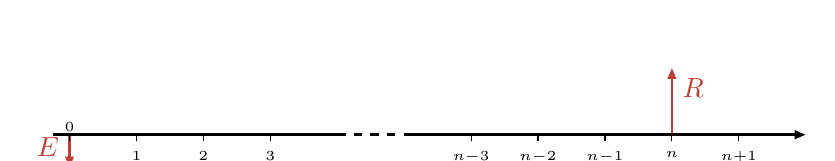
\begin{tikzpicture}[scale=0.85]
    % Draw the x-axis and y-axis.
    \def\w{11}
    \def\n{9}
    \draw[ line width=1, color=OrangeProfondIRA, arrows={-Stealth[length=4, inset=0]}] (0,0) -- (0,-0.4909) node[above left] (A) {$E$};	
    \foreach \y in  {0,...,3} {
        \draw (\y,0) -- (\y,-0.1);
        \ifthenelse{\y>0 }{	\node[below] at (\y,-0.1) {\tiny $ \scriptstyle \y$};
        }{
            \node[above] at (\y,-0.1) {\tiny 0};}
    }
    \foreach \y in  {-3,...,1} {
        \draw (\y+\n,0) -- (\y+\n,-0.1);
        \ifthenelse{\y<0 }{\node[below] at (\y+\n,-0.1) {\tiny $\scriptstyle n \y$};}{}
        \ifthenelse{\y=0 }{\node[below] at (\y+\n,-0.1) {\tiny $\scriptstyle n $};
            \draw[ line width=1, color=OrangeProfondIRA, arrows={-Stealth[length=4, inset=0]}] (\y+\n,0) -- (\y+\n,1) node[below right] (B) {$R$};}{}
        \ifthenelse{\y>0}{	\node[below] at (\y+\n,-0.1) {\tiny $\scriptstyle n+\y$};}{}
    }
    \draw[ line width=1] (-.25,0) -- (4,0);
    \draw[ line width=1, dashed] (4,0) -- (5,0);
    \draw[arrows={-Stealth[length=4, inset=0]}, line width=1] (5,0) -- (\w,0);
\end{tikzpicture}
\end{center}

 Les \textbf{obligations à coupon} :
    \textbf{Les obligations à taux fixe} ont un taux de coupon qui reste constant jusqu'à la date d'échéance.  Avec l'hypothèse d'un remboursement \emph{in fine}, $E$ le prix d'émission, $c$ les coupons et $R$ son remboursement, on peut l'illustrer de la manière suivante :
\begin{center}
\begin{tikzpicture}[scale=0.85]
    % Draw the x-axis and y-axis.
    \def\w{11}
    \def\n{9}
    \draw[ line width=1, color=OrangeProfondIRA, arrows={-Stealth[length=4, inset=0]}] (0,0) -- (0,-1.8) node[above left] (A) {$E$};	
    \foreach \y in  {0,...,3} {
        \draw (\y,0) -- (\y,-0.1);
        \ifthenelse{\y>0 }{	\node[below] at (\y,-0.1) {\tiny $ \scriptstyle \y$};
        \draw[ line width=1, color=OrangeProfondIRA, arrows={-Stealth[length=4, inset=0]}] (\y,0) -- (\y,.25) node [above] {$c$};
        }{
            \node[above] at (\y,-0.1) {\tiny 0};}
        }
    \foreach \y in  {-3,...,1} {
        \draw (\y+\n,0) -- (\y+\n,-0.1);
        \ifthenelse{\y<0 }{\node[below] at (\y+\n,-0.1) {\tiny $\scriptstyle n \y$};
        \draw[ line width=1, color=OrangeProfondIRA, arrows={-Stealth[length=4, inset=0]}] (\y+\n,0) -- (\y+\n,.25) node [above] {$c$};}{}
        \ifthenelse{\y=0 }{\node[below] at (\y+\n,-0.1) {\tiny $\scriptstyle n $};
        \draw[ line width=1, color=OrangeProfondIRA, arrows={-Stealth[length=4, inset=0]}] (\y+\n,0) -- (\y+\n,2) node[below right] (B) {$R$};
        \draw[ line width=1, color=OrangeProfondIRA, arrows={-Stealth[length=4, inset=0]}] (\y+\n,2) -- (\y+\n,2.25) node[right] (B) {$c$};}{}
        \ifthenelse{\y>0}{	\node[below] at (\y+\n,-0.1) {\tiny $\scriptstyle n+\y$};}{}
    }
    \draw[ line width=1] (-.25,0) -- (4,0);
    \draw[ line width=1, dashed] (4,0) -- (5,0);
    \draw[arrows={-Stealth[length=4, inset=0]}, line width=1] (5,0) -- (\w,0);
\end{tikzpicture}
\end{center}

 \textbf{Les obligations indexées} (obligations liées à l'inflation) ont les coupons et parfois aussi la valeur nominale indexés à l'inflation ou à un autre indicateur économique, comme les Obligations Assimilables du Trésor
		indexées sur l'inflation (OATi). Les valeurs de $c$ varient.
        
Les obligations \textbf{à taux flottant}, \textbf{à taux variable} ou \textbf{à taux révisable} : ont un taux de coupon variable lié à un taux d'intérêt de référence (par exemple le euro short-
		term rate (\href{https://www.cmegroup.com/markets/interest-rates/stirs/euro-short-term-rate.quotes.html}{€STR})).

Les obligations \textbf{perpétuelles} n'ont pas de date d'échéance, le principal n'est jamais remboursé.
 
On distingue souvent les obligations d'État (obligations du Trésor, Treasury bonds) des
 obligations d'entreprises ou \engl{corporate} qui sont émises par des entreprises privées.



Une obligation se définit principalement par une \textbf{valeur nominale} $F$ pour \engl{Face Value}), le \textbf{Taux nominal} $i$, sa durée ou \textbf{maturité} $n$.
Dans le cas par défaut, le détenteur de l'obligation confie  le montant $E=F$ à l'émission en 0, reçoit chaque année un coupon $c=i\times F$ et en $n$, le principal ou capital $R=F$ lui est restitué.
Quand $E=F$, on dit que l'émission est au pair, et quand $R=F$, on dit que la restitution est au pair.


Le prix d'une obligation est déterminé par la valeur actuelle des flux de trésorerie futurs attendus (coupons et remboursement du principal) actualisés au taux de rendement du marché $r$.

Le calcul des prix des obligations repose simplement sur la formule de la valeur actualisée :
\[
VP = \sum_{k=1}^{n} \frac{c}{(1 + r)^k} + \frac{F}{(1 + i)^n}
 \]
où :
\begin{itemize}
	\item $VP$ : prix ou valeur présente\index{Valeur Présente} de l'obligation,
	\item $r$ : taux d'intérêt du marché pour la maturité concernée.
\end{itemize}


Pour les obligations à coupons périodiques, le coupon est divisé par le nombre de périodes ($m$) par an et la formule devient :
\[ 
VP = \sum_{k=1}^{mn} \frac{c/m}{(1 + r^{(m)})^k} + \frac{R}{(1 + + r^{(m)})^{mn}}
 \]
 où $c/m$ représente le paiement périodique du coupon et $ r^{(m)}$ le taux d'intérêt périodique.

Le rendement de l'obligation est la valeur $ r^{(m)}$, le taux équivalent de $r$ sur $m$ périodes dans l'année,  qui égalise la valeur présente $VP_r$ avec le prix actuel ou de marché de cette obligation. 

\textbf{La cotation d'une obligation} d'une obligation se fait en pourcentage. Ainsi une cotation à 97,9  sur Euronext indique une valeur de cotation à $97,9 /100\times F$. 
Elle  se fait hors \textbf{coupons courus} , la part du prochain coupon auquel le vendeur a le droit si l'obligation est vendue avant le paiement de ce coupon.
\end{f}
\hrule

\begin{f}[Duration \& Convexité]

La duration de Macaulay :
\[ 		
D = \sum_{t=1}^{n} t \cdot w_t, \quad \text{où} \quad w_t = \frac{PV(C_t)}{P}.
 \]	
Si la fréquence de paiement est $k$ par an, la duration exprimée en années est obtenue en divisant par $k$.
La duration modifiée $D^*$  :
\[ 	
D^* = \frac{D}{1 + i}.
 \]
 Ce qui permet d'approximer la variation du portefeuille $\Delta P$ en cas de variation des taux $\Delta_i$
\[ 
\Delta P \approx -P\ D^* \Delta_i 
 \]
De même, la convexité
\[ 	
C = \frac{1}{P(i)} \times \frac{d^2 P(i)}{di^2},
 \]
 ce qui permet d’affiner l'approximation de $\Delta P$
\[ 	
P(i + \Delta_i) \approx P(i) \left( 1 -D^*\Delta_i + \frac{1}{2} C (\Delta_i)^2 \right).
 \]
\end{f}
\hrule



\begin{f}[MEDAF]
  ou CAPM (\textit{Capital Asset Pricing Model})  :

\[
E(r_i) = r_f + \beta_i (E(r_m) - r_f)
\]

\begin{itemize}
    \item \( E(r_i) \) est le rendement espéré de l'actif \( i \),
    \item \( r_f \) est le taux sans risque,
    \item \( E(r_m) \) est le rendement espéré du marché,
    \item \( \beta_i \) est le coefficient de sensibilité de l'actif \( i \) par rapport aux variations observées sur le marché.
\end{itemize}

Le coefficient \( \beta_i \) mesure la volatilité de l'actif \( i \) par rapport à l'ensemble du marché. 

\end{f}
\hrule


\begin{f}[Marché des dérivés]

Un \textbf{contrat dérivé} (ou actif contingent) est un instrument financier dont la valeur dépend d’un actif ou d’une variable sous-jacente. Les options font partie des contrats dérivés.


Une \textbf{option} est un contrat donnant le droit (sans obligation) d’acheter (call) ou de vendre (put) un actif sous-jacent à un prix fixé (prix d’exercice), à une date future, contre paiement d’une prime. 
L’acheteur (position longue) paie la prime ; le vendeur (position courte) la reçoit.L'\textbf{option européenne}  (exercice possible uniquement à l’échéance) et   
 \textbf{option américaine} (exercice possible à tout moment jusqu’à l’échéance).

Les options cotées sur actions sont appelées \textit{stock options}.

\end{f}
\hrule


\begin{f}[Les stratégies simples]

\ %

%\textbf{La position longue sur l'option d'achat}

Avec $T$ l'échéance, $K$ le prix d'exercice, $S$ ou $S_T$ le sous-jacent à l'échéance, le retour (\engl{payoff}) est de $\max (0, S_T-K)=( S_T-K)^{+}$.
En notant $C$ la prime , le profit réalisé est de $\max (0, S_T-K)-C$, avec un profit si  ($S_T<V_{PM}=K + C$)  ($PM$ pour \textbf{point mort}).

		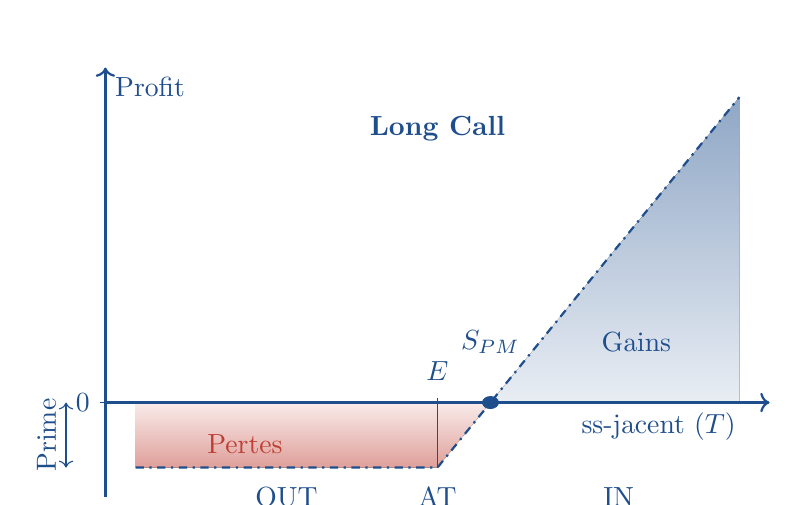
\begin{tikzpicture}[yscale=.75]
\def\riskfreeBS{0.05}
\def\xminBS{5}
\def\xmaxBS{15}
\def\PxExerciceBS{10}
\def\sigmaBS{0.2}
\def\TBS{0.75}
\def\PremiumBS{{BSCall(10,{\PxExerciceBS},{\riskfreeBS},{\TBS},{\sigmaBS})}}
\begin{axis}[ 	extra tick style={tick style=BleuProfondIRA},
clip=false,
axis on top,
axis lines=middle, axis line style={BleuProfondIRA,thick,->},
scale only axis, xmin={\xminBS},xmax={\xmaxBS},enlarge x limits=0.05,
enlarge y limits=0.08,
color=BleuProfondIRA,
%		ylabel near ticks,
ylabel={Profit},
x label style={at={(axis cs:\xmaxBS+.1,0)},anchor=north east},
xlabel={ss-jacent ($T$)},
%		    x label style={at={(axis description cs:0.5,-0.1)},anchor=north},
%		y label style={at={(axis description cs:-0.1,.5)},rotate=90,anchor=south},
ytick=\empty,
xtick=\empty,
extra y ticks ={0},
extra y tick labels={{0}},
extra x ticks ={\PxExerciceBS},
extra x tick labels={{$E$}},
extra x tick style={color=BleuProfondIRA,
	tick label style={yshift=7mm}	},
title ={ \textbf{Long Call}},
%			title style={yshift=-5mm},
%	legend style={draw=none,
	%		legend columns=-1,
	%		at={(0.5,1)},
	%		anchor=south,
	%		outer sep=1em,
	%		node font=\small,
	%	},
]
%		
\addplot[name path=A,BleuProfondIRA,thick,domain={{\xminBS}:{\xmaxBS}}, samples=21,dashdotted] {Call(x,\PxExerciceBS,\PremiumBS)} 
node [pos=0.15,yshift=3mm,color=OrangeProfondIRA] {Pertes}
node [pos=.8,yshift=-15mm,color=BleuProfondIRA] {Gains};	
%\draw[BleuProfondIRA,thick] \OV{\PxExerciceBS}{\PremiumBS}{0.4}{\xminBS}{\xmaxBS} ;
%		\addplot[name path=Option,BleuProfondIRA,thick,domain={250:350}, 			 		samples=10,dashdotted,smooth] {BSPut(x,\PxExerciceBS,\riskfreeBS,\TBS,\sigmaBS)} ;	
\path [save path=\xaxis,name path=xaxis]
({\xminBS},0)		-- ({\xmaxBS},0)		;
\addplot [bottom color=OrangeProfondIRA!50, top color=OrangeProfondIRA!10] fill between [
of=A and xaxis,
split,
every segment no 1/.style=
{top color = BleuProfondIRA!50, bottom color=BleuProfondIRA!10}] ;
%\draw[use path=\xaxis, ->,OrangeProfondIRA,thick];
\draw [fill]  ({-\PremiumBS*(-1)+\PxExerciceBS},0) circle (1mm) node [above=5mm] {$S_{PM}$};
\draw[BleuProfondIRA, thin] ({\PxExerciceBS},0) -- ({\PxExerciceBS},{-\PremiumBS});
\node at ({\xminBS+0.25*(\xmaxBS-\xminBS)},{\pgfkeysvalueof{/pgfplots/ymin}})
{OUT};
\node at ({\PxExerciceBS},{\pgfkeysvalueof{/pgfplots/ymin}})
{AT};
\node at ({\xminBS+0.8*(\xmaxBS-\xminBS)},{\pgfkeysvalueof{/pgfplots/ymin}})
{IN};
\draw [<->, xshift=-5mm] ({\pgfkeysvalueof{/pgfplots/xmin}},0) -- ({\pgfkeysvalueof{/pgfplots/xmin}},-\PremiumBS) node [pos=0.5, xshift=-2.5mm, rotate=90] {Prime};
\end{axis}
%
\end{tikzpicture}


\medskip

%\textbf{La position courte sur l'option d'achat}


À l'échéance, le retour est de $\min (0,K- S_T)=-\max(0, S_T-K)=-( S_T-K)^{+}$ et le profit réalisé est de $C-\max (0, S_T-K)$.

\medskip

			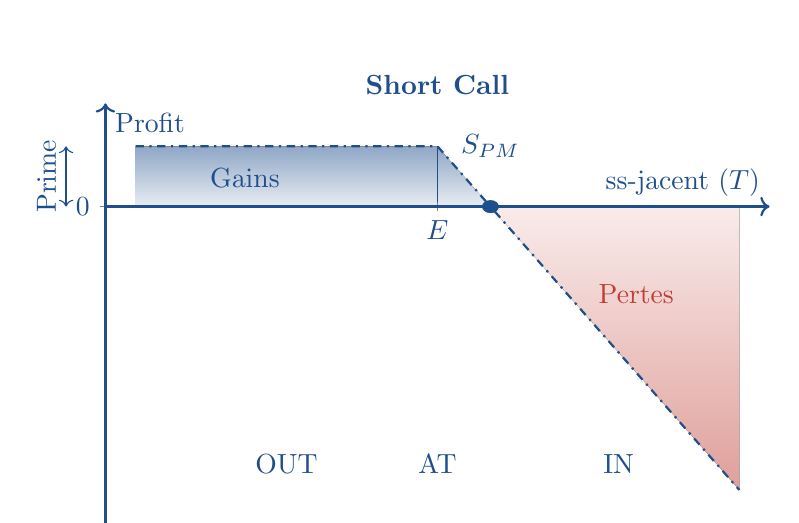
\begin{tikzpicture}[yscale=.75]
		\def\riskfreeBS{0.05}
		\def\xminBS{5}
		\def\xmaxBS{15}
		\def\PxExerciceBS{10}
		\def\sigmaBS{0.2}
		\def\TBS{0.75}
		\def\PremiumBS{{BSCall(10,{\PxExerciceBS},{\riskfreeBS},{\TBS},{\sigmaBS})}}
\begin{axis}[ 
	clip=false,
	axis on top,
	axis lines=middle, axis line style={BleuProfondIRA,thick,->},
	scale only axis, xmin={\xminBS},xmax={\xmaxBS},enlarge x limits=0.05,
	enlarge y limits=0.125,
	color=BleuProfondIRA,
	%		ylabel near ticks,
	ylabel={Profit},
	x label style={={at={(current axis.right of origin)}}},
	%    x label style={at={(axis description cs:1,-0.1)},anchor=south},
	%		x label style={at={(1,0.5)}},
	xlabel={ss-jacent ($T$)},
	%		    x label style={at={(axis description cs:0.5,-0.1)},anchor=north},
	%		y label style={at={(axis description cs:-0.1,.5)},rotate=90,anchor=south},
	ytick=\empty,
	xtick=\empty,
	extra y ticks ={0},
	extra y tick labels={{0}},
	extra x ticks ={\PxExerciceBS},
	extra x tick labels={{$E$}},
	extra x tick style={color=BleuProfondIRA,
		tick label style={yshift=-0mm}	},
	title ={ \textbf{Short Call}},
	title style={yshift=10mm},
	%	legend style={draw=none,
		%		legend columns=-1,
		%		at={(0.5,1)},
		%		anchor=south,
		%		outer sep=1em,
		%		node font=\small,
		%	},
	]
	%		
\addplot[name path=A,BleuProfondIRA,thick,domain={{\xminBS}:{\xmaxBS}}, samples=21,dashdotted] {-Call(x,\PxExerciceBS,\PremiumBS)} 
node [pos=0.15,yshift=-4mm,color=BleuProfondIRA] {Gains}
node [pos=.8,yshift=10mm,color=OrangeProfondIRA] {Pertes};	
	%\draw[BleuProfondIRA,thick] \OV{\PxExerciceBS}{\PremiumBS}{0.4}{\xminBS}{\xmaxBS} ;
	%		\addplot[name path=Option,BleuProfondIRA,thick,domain={250:350}, 			 		samples=10,dashdotted,smooth] {BSPut(x,\PxExerciceBS,\riskfreeBS,\TBS,\sigmaBS)} ;	
	\path [save path=\xaxis,name path=xaxis]
	({\xminBS},0)		-- ({\xmaxBS},0)		;
	\addplot [bottom color=OrangeProfondIRA!50, top color=OrangeProfondIRA!10] fill between [
	of=A and xaxis,
	split,
	every segment no 0/.style=
	{top color = BleuProfondIRA!50, bottom color=BleuProfondIRA!10}] ;
	%\draw[use path=\xaxis, ->,OrangeProfondIRA,thick];
	\draw [fill]  ({-\PremiumBS*(-1)+\PxExerciceBS},0) circle (1mm) node [above=5mm] {$S_{PM}$};
	\draw[BleuProfondIRA, thin] ({\PxExerciceBS},0) -- ({\PxExerciceBS},{\PremiumBS});
	\node at ({\xminBS+0.25*(\xmaxBS-\xminBS)},{\pgfkeysvalueof{/pgfplots/ymin}+1})
	{OUT};
	\node at ({\PxExerciceBS},{\pgfkeysvalueof{/pgfplots/ymin}+1})
	{AT};
	\node at ({\xminBS+0.8*(\xmaxBS-\xminBS)},{\pgfkeysvalueof{/pgfplots/ymin}+01})
	{IN};
	\draw [<->, xshift=-5mm] ({\pgfkeysvalueof{/pgfplots/xmin}},0) -- ({\pgfkeysvalueof{/pgfplots/xmin}},\PremiumBS) node [pos=0.5, xshift=-2.5mm, rotate=90] {Prime};
\end{axis}
%
	\end{tikzpicture}

\medskip


%\textbf{La position longue sur l'option de vente}

À l'échéance, le retour est de $\max (0,K- S_T)=(K- S_T)^{+}$.
En notant $P$ la prime du put, le profit réalisé est de $\max (0,K- S_T)-P$, positif si$V_{PM}=K -P<S_T$.

\medskip

		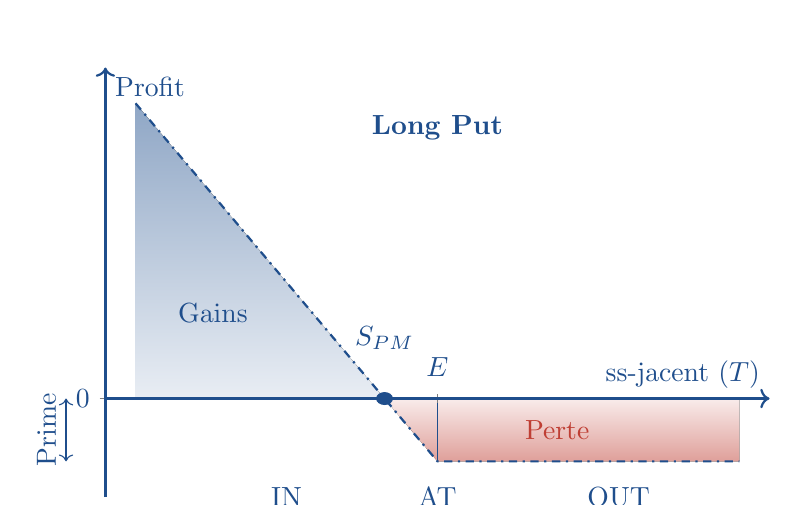
\begin{tikzpicture}[yscale=.75]
	\def\riskfreeBS{0.05}
	\def\xminBS{5}
	\def\xmaxBS{15}
	\def\PxExerciceBS{10}
	\def\sigmaBS{0.2}
	\def\TBS{0.75}
	\def\PremiumBS{{BSCall(10,{\PxExerciceBS},{\riskfreeBS},{\TBS},{\sigmaBS})}}
	\begin{axis}[ 
		clip=false,
		axis on top,
		axis lines=middle, axis line style={BleuProfondIRA,thick,->},
		scale only axis, xmin={\xminBS},xmax={\xmaxBS},enlarge x limits=0.05,
		enlarge y limits=0.1,
		color=BleuProfondIRA,
		%		ylabel near ticks,
		ylabel={Profit},
		x label style={={at={(current axis.right of origin)},below=5mm}},
		%    x label style={at={(axis description cs:1,-0.1)},anchor=south},
		%		x label style={at={(1,0.5)}},
		xlabel={ss-jacent ($T$)},
		%		    x label style={at={(axis description cs:0.5,-0.1)},anchor=north},
		%		y label style={at={(axis description cs:-0.1,.5)},rotate=90,anchor=south},
		ytick=\empty,
		xtick=\empty,
		extra y ticks ={0},
		extra y tick labels={{0}},
		extra x ticks ={\PxExerciceBS},
		extra x tick labels={{$E$}},
		extra x tick style={color=BleuProfondIRA,
			tick label style={yshift=7mm}	},
		title ={ \textbf{Long Put}},
%		title style={yshift=0mm},
		%	legend style={draw=none,
			%		legend columns=-1,
			%		at={(0.5,1)},
			%		anchor=south,
			%		outer sep=1em,
			%		node font=\small,
			%	},
		]		%		
		\addplot[name path=A,BleuProfondIRA,thick,domain={{\xminBS}:{\xmaxBS}}, samples=21,dashdotted] {Put(x,\PxExerciceBS,\PremiumBS)} 
		node [pos=0.15,yshift=-15mm,color=BleuProfondIRA] {Gains}
		node [pos=.75,yshift=4mm,color=OrangeProfondIRA] {Perte};	
		%\draw[BleuProfondIRA,thick] \OV{\PxExerciceBS}{\PremiumBS}{0.4}{\xminBS}{\xmaxBS} ;
		%	\addplot[BleuProfondIRA,thick,dashdotted] {Call(x,50,2)};
		%	\addplot[BleuProfondIRA,thick] {Put(x,50,3)+Call(x,50,2)};
		%\addplot[name path=Option,BleuProfondIRA,thick,domain={250:350}, 			 		samples=10,dashdotted,smooth] {BSPut(x,\PxExerciceBS,\riskfreeBS,\TBS,\sigmaBS)} ;	
		\path [save path=\xaxis,name path=xaxis]
		({\xminBS},0)		-- ({\xmaxBS},0)		;
		\addplot [bottom color=OrangeProfondIRA!50, top color=OrangeProfondIRA!10] fill between [
		of=A and xaxis,
		split,
		every segment no 0/.style=
		{top color = BleuProfondIRA!50, bottom color=BleuProfondIRA!10}] ;
		%\draw[use path=\xaxis, ->,OrangeProfondIRA,thick];
		\draw [fill]  ({-\PremiumBS+\PxExerciceBS},0) circle (1mm) node [above=5mm] {$S_{PM}$};
		\draw[BleuProfondIRA, thin] ({\PxExerciceBS},0) -- ({\PxExerciceBS},{-\PremiumBS});
		\node at ({\xminBS+0.25*(\xmaxBS-\xminBS)},{\pgfkeysvalueof{/pgfplots/ymin}})
		{IN};
		\node at ({\PxExerciceBS},{\pgfkeysvalueof{/pgfplots/ymin}})
		{AT};
		\node at ({\xminBS+0.8*(\xmaxBS-\xminBS)},{\pgfkeysvalueof{/pgfplots/ymin}})
		{OUT};
		\draw [<->, xshift=-5mm] ({\pgfkeysvalueof{/pgfplots/xmin}},0) -- ({\pgfkeysvalueof{/pgfplots/xmin}},-\PremiumBS) node [pos=0.5, xshift=-2.5mm, rotate=90] {Prime};
	\end{axis}
	%
\end{tikzpicture}

    	     

%\textbf{La position courte sur l'option de vente}

\medskip

		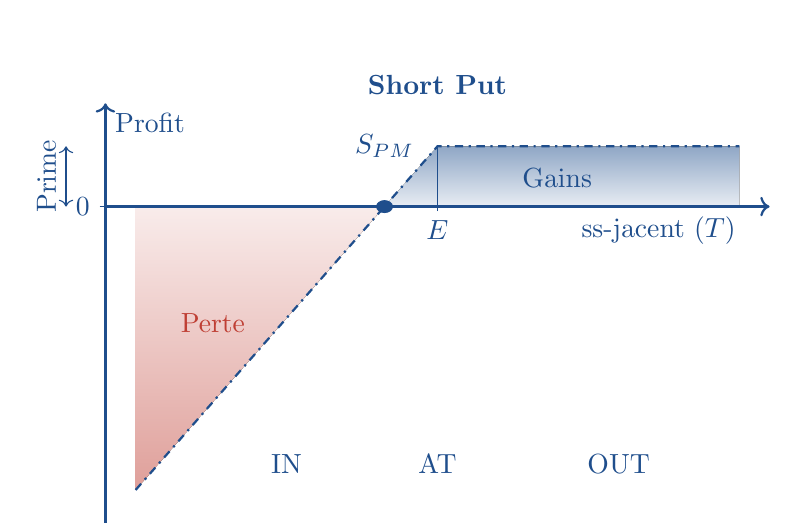
\begin{tikzpicture}[yscale=.75]
	\def\riskfreeBS{0.05}
	\def\xminBS{5}
	\def\xmaxBS{15}
	\def\PxExerciceBS{10}
	\def\sigmaBS{0.2}
	\def\TBS{0.75}
	\def\PremiumBS{{BSCall(10,{\PxExerciceBS},{\riskfreeBS},{\TBS},{\sigmaBS})}}
	\begin{axis}[ 	extra tick style={tick style=BleuProfondIRA},
		clip=false,
		axis on top,
		axis lines=middle, axis line style={BleuProfondIRA,thick,->},
		scale only axis, xmin={\xminBS},xmax={\xmaxBS},enlarge x limits=0.05,
		enlarge y limits=0.125,
		color=BleuProfondIRA,
		%		ylabel near ticks,
		ylabel={Profit},
x label style={at={(axis cs:\xmaxBS+.1,0)},anchor=north east},
		xlabel={ss-jacent ($T$)},
		%		    x label style={at={(axis description cs:0.5,-0.1)},anchor=north},
		%		y label style={at={(axis description cs:-0.1,.5)},rotate=90,anchor=south},
		ytick=\empty,
		xtick=\empty,
		extra y ticks ={0},
		extra y tick labels={{0}},
		extra x ticks ={\PxExerciceBS},
		extra x tick labels={{$E$}},
		extra x tick style={color=BleuProfondIRA,
			tick label style={yshift=0mm}	},
		title ={ \textbf{Short Put}},
		title style={yshift=10mm},
		%	legend style={draw=none,
			%		legend columns=-1,
			%		at={(0.5,1)},
			%		anchor=south,
			%		outer sep=1em,
			%		node font=\small,
			%	},
		]		%		
		\addplot[name path=A,BleuProfondIRA,thick,domain={{\xminBS}:{\xmaxBS}}, samples=21,dashdotted] {-Put(x,\PxExerciceBS,\PremiumBS)} 
		node [pos=0.15,yshift=10mm,color=OrangeProfondIRA] {Perte}
		node [pos=.75,yshift=-4mm,color=BleuProfondIRA] {Gains};	
		%\draw[BleuProfondIRA,thick] \OV{\PxExerciceBS}{\PremiumBS}{0.4}{\xminBS}{\xmaxBS} ;
		%	\addplot[BleuProfondIRA,thick,dashdotted] {Call(x,50,2)};
		%	\addplot[BleuProfondIRA,thick] {Put(x,50,3)+Call(x,50,2)};
		%\addplot[name path=Option,BleuProfondIRA,thick,domain={250:350}, 			 		samples=10,dashdotted,smooth] {BSPut(x,\PxExerciceBS,\riskfreeBS,\TBS,\sigmaBS)} ;	
		\path [save path=\xaxis,name path=xaxis]
		({\xminBS},0)		-- ({\xmaxBS},0)		;
		\addplot [bottom color=OrangeProfondIRA!50, top color=OrangeProfondIRA!10] fill between [
		of=A and xaxis,
		split,
		every segment no 1/.style=
		{top color = BleuProfondIRA!50, bottom color=BleuProfondIRA!10}] ;
		%\draw[use path=\xaxis, ->,OrangeProfondIRA,thick];
		\draw [fill]  ({-\PremiumBS+\PxExerciceBS},0) circle (1mm) node [above=5mm] {$S_{PM}$};
		\draw[BleuProfondIRA, thin] ({\PxExerciceBS},0) -- ({\PxExerciceBS},{\PremiumBS});
		\node at ({\xminBS+0.25*(\xmaxBS-\xminBS)},{\pgfkeysvalueof{/pgfplots/ymin}+1})
		{IN};
		\node at ({\PxExerciceBS},{\pgfkeysvalueof{/pgfplots/ymin}+1})
		{AT};
		\node at ({\xminBS+0.8*(\xmaxBS-\xminBS)},{\pgfkeysvalueof{/pgfplots/ymin}+1})
		{OUT};
		\draw [<->, xshift=-5mm] ({\pgfkeysvalueof{/pgfplots/xmin}},0) -- ({\pgfkeysvalueof{/pgfplots/xmin}},\PremiumBS) node [pos=0.5, xshift=-2.5mm, rotate=90] {Prime};
	\end{axis}
	%
\end{tikzpicture}
    	     

À l'échéance, le retour est de $\min (0, S_T-K)=-(K- S_T)^+$.


\end{f}
\hrule

\begin{f}[Les stratégies d'écart]
\textbf{Stratégie d'écart} : utilise deux options ou plus du même type (deux options d'achat ou deux options de vente).  
Si les prix d'exercice varient, c'est un \textbf{écart vertical}.  
Si les échéances changent, c'est un \textbf{écart horizontal}.

Une stratégie d’écart vertical (\textit{spread trading strategy}) implique une position longue et une position courte sur des options d’achat portant sur le même sous-jacent, de même échéance mais avec des prix d’exercice différents.  
On distingue : \textbf{écart vertical haussier} (\textit{Bull spread}) et \textbf{écart vertical baissier} (\textit{Bear spread}).

\textbf{Écart vertical haussier} : anticipant une hausse modérée du sous-jacent, l’investisseur prend une position longue sur $C_1$ et courte sur $C_2$ sous la contrainte $E_1 < E_2$.  
Résultat net à l’échéance :

	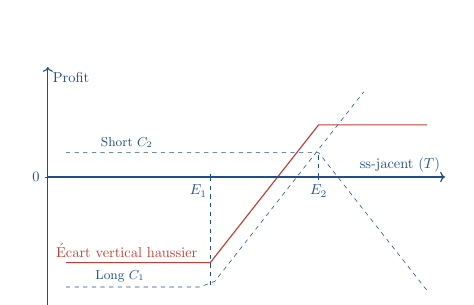
\begin{tikzpicture}[scale=.52]
		\def\riskfreeBS{0.05}
		\def\xminBS{5}
		\def\xmaxBS{15}
		\def\PxExerciceBSa{9}
		\def\PxExerciceBSb{12}
		\def\sigmaBS{0.2}
		\def\TBS{0.75}
		\def\PremiumBSa{{BSCall(11,{\PxExerciceBSa},{\riskfreeBS},{\TBS},{\sigmaBS})}}
		\def\PremiumBSb{{BSCall(11,{\PxExerciceBSb},{\riskfreeBS},{\TBS},{\sigmaBS})}}
		\begin{axis}[ 
			width=0.8\textwidth,
			height=0.5\textwidth, 
			extra tick style={tick style=BleuProfondIRA},
			clip=false,
			axis on top,
			axis lines=middle, axis line style={BleuProfondIRA,thick,->},
			scale only axis, xmin={\xminBS},xmax={\xmaxBS},enlarge x limits=0.05,
			enlarge y limits=0.125,
			color=BleuProfondIRA,
			%		ylabel near ticks,
			ylabel={Profit},
			x label style={={at={(current axis.right of origin)}}},
			%    x label style={at={(axis description cs:1,-0.1)},anchor=south},
			%		x label style={at={(1,0.5)}},
			xlabel={ss-jacent ($T$)},
			%		    x label style={at={(axis description cs:0.5,-0.1)},anchor=north},
			%		y label style={at={(axis description cs:-0.1,.5)},rotate=90,anchor=south},
			ytick=\empty,
			xtick=\empty,
			extra y ticks ={0},
			extra y tick labels={{0}},
			extra x ticks ={{\PxExerciceBSa},{\PxExerciceBSb}},
			extra x tick labels={{$E_1\ \ \ \ \ $},{$E_2$}},
			extra x tick style={color=BleuProfondIRA,
				tick label style={yshift=-0mm}	},
			]
			%		
			\addplot[name path=A,BleuProfondIRA,thin,domain={{\xminBS}:{\xmaxBS-1.75}}, samples=21,dashed] {Call(x,\PxExerciceBSa,\PremiumBSa)} 
			node [pos=0.15, above] {\small Long $C_1$};	
			\addplot[name path=B,BleuProfondIRA,thin,domain={{\xminBS}:{\xmaxBS}}, samples=21,dashed] {-Call(x,\PxExerciceBSb,\PremiumBSb)} 
			node [pos=0.15, above] {\small  Short $C_2$};	
			\addplot[name path=EVH,OrangeProfondIRA,thick,domain={{\xminBS}:{\xmaxBS}}, samples=41] {Call(x,\PxExerciceBSa,\PremiumBSa)-Call(x,\PxExerciceBSb,\PremiumBSb)} node [pos=0.15, above] {\'Ecart vertical haussier};	
			%\draw[BleuProfondIRA,thick] \OV{\PxExerciceBSa}{\PremiumBSa}{0.4}{\xminBS}{\xmaxBS} ;
			%		\addplot[name path=Option,BleuProfondIRA,thick,domain={250:350}, 			 		samples=10,dashdotted,smooth] {BSPut(x,\PxExerciceBSa,\riskfreeBS,\TBS,\sigmaBS)} ;	
			
			\draw[BleuProfondIRA, thin, dashed] ({\PxExerciceBSa},0) -- ({\PxExerciceBSa},{-\PremiumBSa})	;
			\draw[BleuProfondIRA, thin, dashed] ({\PxExerciceBSb},0) -- ({\PxExerciceBSb},{\PremiumBSb})	;
		\end{axis}
		%
	\end{tikzpicture}



\textbf{Écart vertical baissier} : anticipant une baisse modérée du sous-jacent, l’investisseur vend l’option la plus chère et achète la moins chère.


	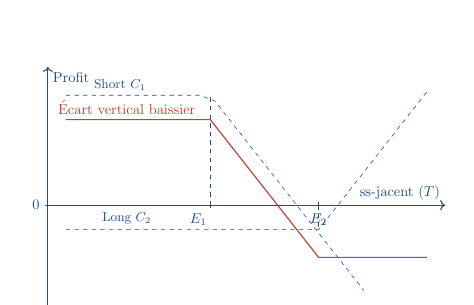
\begin{tikzpicture}[scale=.52]
		\def\riskfreeBS{0.05}
		\def\xminBS{5}
		\def\xmaxBS{15}
		\def\PxExerciceBSa{9}
		\def\PxExerciceBSb{12}
		\def\sigmaBS{0.2}
		\def\TBS{0.75}
		\def\PremiumBSa{{BSCall(11,{\PxExerciceBSa},{\riskfreeBS},{\TBS},{\sigmaBS})}}
		\def\PremiumBSb{{BSCall(11,{\PxExerciceBSb},{\riskfreeBS},{\TBS},{\sigmaBS})}}
		\begin{axis}[ 
			width=0.8\textwidth,
			height=0.5\textwidth, 
			extra tick style={tick style=BleuProfondIRA},
			clip=false,
			axis on top,
			axis lines=middle, axis line style={BleuProfondIRA,thick,->},
			scale only axis, xmin={\xminBS},xmax={\xmaxBS},enlarge x limits=0.05,
			enlarge y limits=0.125,
			color=BleuProfondIRA,
			%		ylabel near ticks,
			ylabel={Profit},
			x label style={={at={(current axis.right of origin)}}},
			%    x label style={at={(axis description cs:1,-0.1)},anchor=south},
			%		x label style={at={(1,0.5)}},
			xlabel={ss-jacent ($T$)},
			%		    x label style={at={(axis description cs:0.5,-0.1)},anchor=north},
			%		y label style={at={(axis description cs:-0.1,.5)},rotate=90,anchor=south},
			ytick=\empty,
			xtick=\empty,
			extra y ticks ={0},
			extra y tick labels={{0}},
			extra x ticks ={{\PxExerciceBSa},{\PxExerciceBSb}},
			extra x tick labels={{$E_1\ \ \ \ \ $},{$E_2$}},
			extra x tick style={color=BleuProfondIRA,
				tick label style={yshift=-0mm}	},
			]
			%		
			\addplot[name path=A,BleuProfondIRA,thin,domain={{\xminBS}:{\xmaxBS-1.75}}, samples=21,dashed] {-Call(x,\PxExerciceBSa,\PremiumBSa)} 
			node [pos=0.15, above] {\small Short $C_1$};	
			\addplot[name path=B,BleuProfondIRA,thin,domain={{\xminBS}:{\xmaxBS}}, samples=21,dashed] {Call(x,\PxExerciceBSb,\PremiumBSb)} 
			node [pos=0.15, above] {\small  Long $C_2$};		
			\addplot[name path=EVH,OrangeProfondIRA,thick,domain={{\xminBS}:{\xmaxBS}}, samples=41] {-Call(x,\PxExerciceBSa,\PremiumBSa)+Call(x,\PxExerciceBSb,\PremiumBSb)} node [pos=0.15, above] {\'Ecart vertical baissier};	
			%\draw[BleuProfondIRA,thick] \OV{\PxExerciceBSa}{\PremiumBSa}{0.4}{\xminBS}{\xmaxBS} ;
			%		\addplot[name path=Option,BleuProfondIRA,thick,domain={250:350}, 			 		samples=10,dashdotted,smooth] {BSPut(x,\PxExerciceBSa,\riskfreeBS,\TBS,\sigmaBS)} ;	
			
			\draw[BleuProfondIRA, thin, dashed] ({\PxExerciceBSa},0) -- ({\PxExerciceBSa},{\PremiumBSa})	;
			\draw[BleuProfondIRA, thin, dashed] ({\PxExerciceBSb},0) -- ({\PxExerciceBSb},{-\PremiumBSb})	;
		\end{axis}
		%
	\end{tikzpicture}

% Code TikZ conservé ici (éventuellement inséré)

\textbf{Écart papillon} (\textit{butterfly spread}) : anticipe une faible variation du sous-jacent.  
C’est la combinaison d’un écart vertical haussier et d’un écart vertical baissier.  
Stratégie adaptée si de grandes variations sont jugées peu probables.  
Investissement initial faible.

	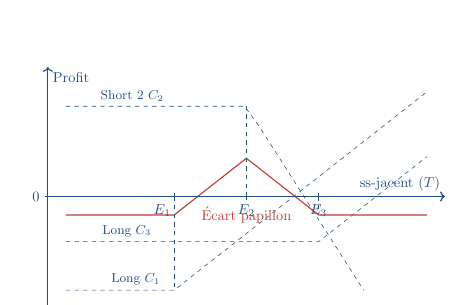
\begin{tikzpicture}[scale=.52]
		\def\riskfreeBS{0.05}
		\def\xminBS{5}
		\def\xmaxBS{15}
		\def\PxExerciceBSa{8}
		\def\PxExerciceBSb{10}
		\def\PxExerciceBSc{12}
		\def\sigmaBS{0.2}
		\def\TBS{0.75}
		\def\PremiumBSa{BSCall(11,{\PxExerciceBSa},{\riskfreeBS},{\TBS},{\sigmaBS})}
		\def\PremiumBSb{BSCall(11,{\PxExerciceBSb},{\riskfreeBS},{\TBS},{\sigmaBS})}
		\def\PremiumBSc{BSCall(11,{\PxExerciceBSc},{\riskfreeBS},{\TBS},{\sigmaBS})}
		\begin{axis}[
			width=0.8\textwidth,
			height=0.5\textwidth, 
			extra tick style={tick style=BleuProfondIRA},
			clip=false,
			axis on top,
			axis lines=middle, axis line style={BleuProfondIRA,thick,->},
			scale only axis, xmin={\xminBS},xmax={\xmaxBS},enlarge x limits=0.05,
			enlarge y limits=0.125,
			color=BleuProfondIRA,
			%		ylabel near ticks,
			ylabel={Profit},
			x label style={={at={(current axis.right of origin)}}},
			%    x label style={at={(axis description cs:1,-0.1)},anchor=south},
			%		x label style={at={(1,0.5)}},
			xlabel={ss-jacent ($T$)},
			%		    x label style={at={(axis description cs:0.5,-0.1)},anchor=north},
			%		y label style={at={(axis description cs:-0.1,.5)},rotate=90,anchor=south},
			ytick=\empty,
			xtick=\empty,
			extra y ticks ={0},
			extra y tick labels={{0}},
			extra x ticks ={{\PxExerciceBSa},{\PxExerciceBSb},{\PxExerciceBSc}},
			extra x tick labels={{$E_1\ \ \ \ \ $},{$E_2$},{$E_3$}},
			extra x tick style={color=BleuProfondIRA,
				tick label style={yshift=-0mm}	},
			]
			%		
			\addplot[name path=A,BleuProfondIRA,thin,domain={{\xminBS}:{\xmaxBS}}, samples=21,dashed] {Call(x,\PxExerciceBSa,\PremiumBSa)} 
			node [pos=0.15, above] {\small Long $C_1$};	
			\addplot[name path=B,BleuProfondIRA,thin,domain={{\xminBS}:{\xmaxBS-1.75}}, samples=21,dashed] {-2*Call(x,\PxExerciceBSb,\PremiumBSb)} 
			node [pos=0.15, above] {\small Short $2\ C_2$};	
			\addplot[name path=C,BleuProfondIRA,thin,domain={{\xminBS}:{\xmaxBS}}, samples=21,dashed] {Call(x,\PxExerciceBSc,\PremiumBSb)} 
			node [pos=0.15, above] {\small Long $C_3$};	
			\addplot[name path=EP,OrangeProfondIRA,thick,domain={{\xminBS}:{\xmaxBS}}, samples=41] {
				Call(x,\PxExerciceBSa,\PremiumBSa) - 2*Call(x,\PxExerciceBSb,\PremiumBSb)+
				Call(x,\PxExerciceBSc,\PremiumBSc)}
			node [pos=0.5, below=30pt] { \'Ecart papillon};	
			\draw[BleuProfondIRA, thin, dashed] ({\PxExerciceBSa},0) -- ({\PxExerciceBSa},{-\PremiumBSa})	;
			\draw[BleuProfondIRA, thin, dashed] ({\PxExerciceBSb},0) -- ({\PxExerciceBSb},{2*\PremiumBSb})	;
			\draw[BleuProfondIRA, thin, dashed] ({\PxExerciceBSc},0) -- ({\PxExerciceBSc},{-\PremiumBSc})	;
		\end{axis}
		%
	\end{tikzpicture}
% Code TikZ conservé ici (éventuellement inséré)

\end{f}
\hrule

\begin{f}[Les stratégies combinées]
	
	Une \textbf{stratégie combinée} utilise à la fois des options d'achat et de vente. On distingue notamment les \textbf{stellages} et les \textbf{strangles}.
	
	Un \textbf{stellage} (straddle) combine l'achat d'une option d'achat et d'une option de vente de même échéance et de même prix d'exercice. Cette stratégie parie sur une forte variation du prix, à la hausse ou à la baisse. La perte maximale survient si le prix à l’échéance est égal au prix d’exercice.
	
	Un \textbf{strangle} est l’achat d’un call et d’un put de même échéance mais à prix d’exercice différents. Il suppose une très forte variation de la valeur du sous-jacent.
	
		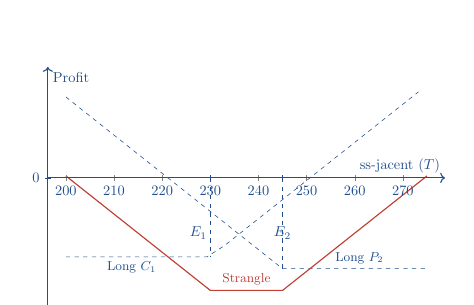
\begin{tikzpicture}[scale=.52]
			\def\xminBS{200}
			\def\xmaxBS{275}
			\def\PxExerciceBSa{230}
			\def\PxExerciceBSb{245}
			\def\PremiumBSa{20.69}
			\def\PremiumBSb{23.79}
			\begin{axis}[ 
				width=0.8\textwidth,
				height=0.5\textwidth, 
				extra tick style={tick style=BleuProfondIRA},
				clip=false,
				axis on top,
				axis lines=middle, axis line style={BleuProfondIRA,thick,->},
				scale only axis, xmin={\xminBS},xmax={\xmaxBS},enlarge x limits=0.05,
				enlarge y limits=0.125,
				color=BleuProfondIRA,
				ylabel={Profit},
				x label style={={at={(current axis.right of origin)}}},
				xlabel={ss-jacent ($T$)},
				ytick=\empty,
				extra y ticks ={0},
				extra y tick labels={{0}},
				extra x ticks ={{\PxExerciceBSa},{\PxExerciceBSb}},
				extra x tick labels={{$E_1\ \ \ \ \ $},{$E_2$}},
				extra x tick style={color=BleuProfondIRA,
					tick label style={yshift=-10mm}	},
				]
				\addplot[name path=A,BleuProfondIRA,thin,domain={{\xminBS}:{\xmaxBS-1.75}}, samples=21,dashed] {Call(x,\PxExerciceBSa,\PremiumBSa)} 
				node [pos=0.15, below] {\small Long $C_1$};	
				\addplot[name path=B,BleuProfondIRA,thin,domain={{\xminBS}:{\xmaxBS}}, samples=21,dashed] {Put(x,\PxExerciceBSb,\PremiumBSb)} 
				node [pos=0.85, above] {\small  Long $P_2$};		
				\addplot[name path=EVH,OrangeProfondIRA,thick,domain={{\xminBS}:{\xmaxBS}}, samples=21] {Call(x,\PxExerciceBSa,\PremiumBSa)+Put(x,\PxExerciceBSb,\PremiumBSb)} node [pos=0.5, above] {\small Strangle};	
				\draw[BleuProfondIRA, thin, dashed] ({\PxExerciceBSa},0) -- ({\PxExerciceBSa},{-\PremiumBSa})	;
				\draw[BleuProfondIRA, thin, dashed] ({\PxExerciceBSb},0) -- ({\PxExerciceBSb},{-\PremiumBSb})	;
			\end{axis}
		\end{tikzpicture}


		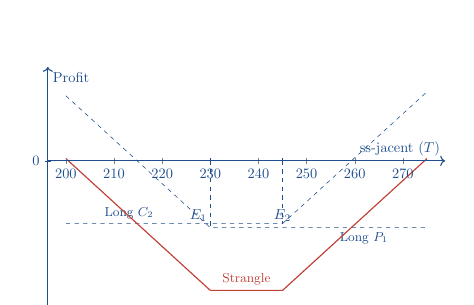
\begin{tikzpicture}[scale=.52]
			\def\xminBS{200}
			\def\xmaxBS{275}
			\def\PxExerciceBSa{230}
			\def\PxExerciceBSb{245}
			\def\PremiumBSa{15.19}
			\def\PremiumBSb{14.29}
			\begin{axis}[ 
				width=0.8\textwidth,
				height=0.5\textwidth, 
				extra tick style={tick style=BleuProfondIRA},
				clip=false,
				axis on top,
				axis lines=middle, axis line style={BleuProfondIRA,thick,->},
				scale only axis, xmin={\xminBS},xmax={\xmaxBS},enlarge x limits=0.05,
				enlarge y limits=0.125,
				color=BleuProfondIRA,
				ylabel={Profit},
				x label style={={at={(current axis.right of origin)}}},
				xlabel={ss-jacent ($T$)},
				ytick=\empty,
				extra y ticks ={0},
				extra y tick labels={{0}},
				extra x ticks ={{\PxExerciceBSa},{\PxExerciceBSb}},
				extra x tick labels={{$E_1\ \ \ \ \ $},{$E_2$}},
				extra x tick style={color=BleuProfondIRA,
					tick label style={yshift=-10mm}	},
				]
				\addplot[name path=A,BleuProfondIRA,thin,domain={{\xminBS}:{\xmaxBS}}, samples=21,dashed] {Put(x,\PxExerciceBSa,\PremiumBSa)} 
				node [pos=0.85, below] {\small Long $P_1$};	
				\addplot[name path=B,BleuProfondIRA,thin,domain={{\xminBS}:{\xmaxBS}}, samples=21,dashed] {Call(x,\PxExerciceBSb,\PremiumBSb)} 
				node [pos=0.15, above] {\small  Long $C_2$};		
				\addplot[name path=EVH,OrangeProfondIRA,thick,domain={{\xminBS}:{\xmaxBS}}, samples=21] {Put(x,\PxExerciceBSa,\PremiumBSa)+Call(x,\PxExerciceBSb,\PremiumBSb)} node [pos=0.5, above] {\small Strangle};	
				\draw[BleuProfondIRA, thin, dashed] ({\PxExerciceBSa},0) -- ({\PxExerciceBSa},{-\PremiumBSa})	;
				\draw[BleuProfondIRA, thin, dashed] ({\PxExerciceBSb},0) -- ({\PxExerciceBSb},{-\PremiumBSb})	;
			\end{axis}
		\end{tikzpicture}
	
	
	
\end{f}
\hrule

\begin{f}[Absence d'opportunité d'arbitrage]
Aucun profit sans risque n’est possible par exploitation des écarts de prix. 

\end{f}

\begin{f}[La relation de parité]

L'AOA implique la relation suivante entre le Call et le Put :

$$S_t- C_t + P_t = K e^{-i_{f}.\tau}$$	
\end{f}
\hrule

\begin{f}[Le modèle de Cox-Ross-Rubinstein]
	
Il repose sur un processus en temps discret avec deux évolutions possibles du prix à chaque période : une hausse (facteur $u$) ou une baisse (facteur $d$), avec $u > 1 + i_{f}$ et $d < 1 + i_{f}$. Le prix à $t = 1$ est alors \( S_{1}^{u} = S_{0} u \) ou \( S_{1}^{d} = S_{0} d \), selon une probabilité $q$ ou $1-q$.

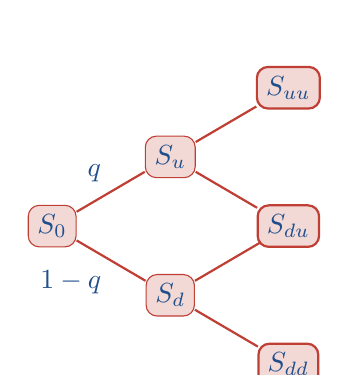
\begin{tikzpicture}
	[sibling distance=5em,
	every node/.style = {shape=rectangle, rounded corners, fill=OrangeProfondIRA!20,
		align=center,  draw=OrangeProfondIRA, text=BleuProfondIRA } ,grow=right,
	edge from parent/.style={draw=OrangeProfondIRA, thick}]
	\node (A){$S_0$}
	child {node  (B) {$S_d$}
		child {node {$S_{dd}$}}
		child} 
	child {node (C) {$S_u$} 
		child {node  {$S_{du}$}}
		child {node {$S_{uu}$}}    
	};
	\draw [draw=none] 
	($ (A.east) + (0,0.2) $) -- node[draw=none, fill=none, above left, BleuProfondIRA] {$q$} ($ (C.west) + (0,-0.2) $);
	\draw [draw=none]  
	($ (A.east) + (0,-0.2) $) -- node[draw=none, fill=none,below left, BleuProfondIRA] {$1 - q$} ($ (B.west) + (0,0.2) $);
\end{tikzpicture}
\quad
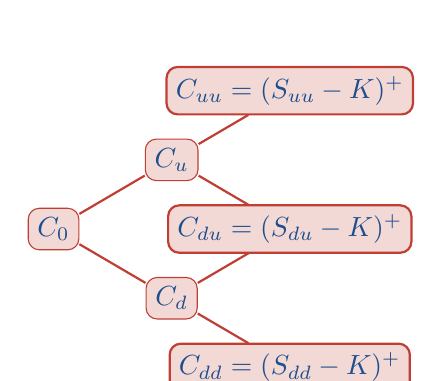
\begin{tikzpicture}
	[sibling distance=5em,
	every node/.style = {shape=rectangle, rounded corners, fill=OrangeProfondIRA!20,
		align=center,  draw=OrangeProfondIRA, text=BleuProfondIRA } ,grow=right,
	edge from parent/.style={draw=OrangeProfondIRA, thick}]
	\node {$C_0$}
	child {node  {$C_d$}
		child {node {$C_{dd}=(S_{dd}-K)^{+}$}}
		child}
	child {node {$C_u$} 
		child {node  {$C_{du}=(S_{du}-K)^{+}$}}
		child {node  {$C_{uu}=(S_{uu}-K)^{+}$}}  
	};
\end{tikzpicture}

Ce modèle s’étend à $n$ périodes avec $n+1$ prix possibles pour $S_T$. À l’échéance, la valeur d’une option d’achat est donnée par \( C_{1}^{u} = (S_{1}^{u} - K)^+ \) et \( C_{1}^{d} = (S_{1}^{d} - K)^+ \).

\textbf{Absence d'opportunité d'arbitrage} implique
\[
d < 1 + i_{f} < u
\]
et une probabilité risque neutre 
\[q = \frac{(1 + i_{f}) - d}{u - d}\]

\textbf{Prix du call} (avec \( S_{1}^{d} < K < S_{1}^{u} \)) :
\[
C_{0} = \frac{1}{1+i_f} \left[ q C_{1}^{u} + (1 - q) C_{1}^{d} \right]
\]

On peut aussi construire un portefeuille de réplication composé de $\Delta$ actions et $B$ obligations, tel que :
\[
\begin{cases}
	\Delta = \frac{S_{1}^{u} - K}{S_{1}^{u} - S_{1}^{d}}, \\
	B = \frac{-S_{1}^{d}}{1+i_f} \cdot \Delta
\end{cases}
\quad \Rightarrow \quad \Pi_0 = \Delta S_0 + B
\]

\textbf{Prix du put} :
\[
P_{0} = \frac{1}{1+i_f} \left[ q P_{1}^{u} + (1 - q) P_{1}^{d} \right]
\]

\textbf{Détermination de $q$, $u$, $d$} :  
En calibrant le modèle pour retrouver les premiers moments du rendement sous la probabilité risque neutre (espérance $i_f$, variance $\sigma^2 \delta t$), on obtient :
\[
e^{i_{f} \delta t} = q u + (1-q) d, \qquad q u^2 + (1-q) d^2 - [q u + (1-q) d]^2 = \sigma^2 \delta t
\]

Avec la contrainte $u = \frac{1}{d}$, on arrive à :
\[
\begin{array}{l}
	q = \frac{e^{-i_f \delta_t} - d}{u - d} \\
	u = e^{\sigma \sqrt{\delta t}} \\
	d = e^{-\sigma \sqrt{\delta t}}
\end{array}
\]

\end{f}
\hrule

\begin{f}[Le modèle de Black \& Scholes]
Hypothèses du modèle 
\begin{itemize}
	\item Le taux sans risque $R$ est constant. On définit $i_f = \ln(1+R)$, ce qui implique $(1+R)^t = e^{i_f t}$.
	\item Le prix de l'action $S_t$ suit un mouvement brownien géométrique :
	$$
	dS_t = \mu S_t dt + \sigma S_t dW_t 
	$$
	$$
	 S_t = S_0 \exp\left(\sigma W_t + \left( \mu - \frac{1}{2}\sigma^2 \right)t \right)
	$$
	\item Pas de dividende pendant la durée de vie de l’option.
	\item L’option est \og{}européenne\fg{} (exercée uniquement à l’échéance).
	\item Marché sans friction : pas d’impôts ni de coûts de transaction.
	\item La vente à découvert est autorisée.
\end{itemize}

L’équation de Black-Scholes-Merton pour évaluer un contrat dérivé $f$ est :
$$
\frac{\partial f}{\partial t} + i_f S \frac{\partial f}{\partial S} + \frac{1}{2}\sigma^2 S^2 \frac{\partial^2 f}{\partial S^2} = i_f f
$$

À l’échéance, le prix d’une option d’achat est $C(S,T) = \max(0, S_T - K)$, et celui d’une option de vente est $P(S,T) = \max(0, K - S_T)$.


\begin{center}
	\begin{tabular}{|c|c|c|}
		\hline
		Déterminants & \textbf{call}&\textbf{put}\\
		\hline
		Cours du sous-jacent	      & +&	-\\
		Prix d'exercice	              & -&	+\\
		La maturité	 (ou le temps)    & + (-)&	+ (-)\\
		Volatilité	              & +&	+\\
		Taux d'intérêt à court terme  & +&	-\\
		Versement de dividende	      & -&	+\\
		\hline
	\end{tabular}
\end{center}

Les solutions analytiques sont :
\begin{align*}
	C_t &= S_t \Phi(d_1) - Ke^{-i_f \tau} \Phi(d_2) \\
	P_t &= Ke^{-i_f \tau} \Phi(-d_2) - S_t \Phi(-d_1)
\end{align*}
où :
\begin{align*}
	d_1 &= \frac{\ln(S_t/K) + (i_f + \frac{1}{2}\sigma^2)\tau}{\sigma \sqrt{\tau}}, \quad
	d_2 = d_1 - \sigma \sqrt{\tau}
\end{align*}

%La sensibilité peut être mesurée par cinq paramètres (lettres grecques) :

\begin{itemize}
	\item \textbf{Delta} $\Delta$ : variation du prix de l’option selon le sous-jacent.
	\item \textbf{Gamma} $\Gamma$ : sensibilité du delta.
	\item \textbf{Thêta} $\Theta$ : sensibilité au temps.
	\item \textbf{Véga} $\mathcal{V}$ : sensibilité à la volatilité.
	\item \textbf{Rho} $\rho$ : sensibilité au taux d’intérêt.
\end{itemize}


Le \textbf{Delta} mesure l’impact d’une variation du sous-jacent :

\begin{align*}
	\Delta_C &= \frac{\partial C}{\partial S} = \Phi(d_1), \quad \Delta \in (0,1) \\
	\Delta_P &= \frac{\partial P}{\partial S} = \Phi(d_1) - 1, \quad \Delta \in (-1,0)
\end{align*}


Le Delta global d’un portefeuille $\Pi$ avec des poids $\omega_i$ est :
$$
\frac{\partial \Pi}{\partial S_t} = \sum_{i=1}^{n} \omega_i \Delta_i
$$



% Graphique TikZ conservé tel quel :

\begin{center}
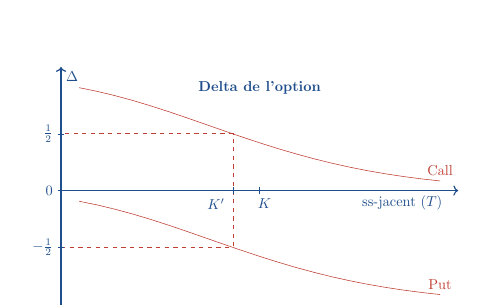
\begin{tikzpicture}[scale=.52]
\def\riskfreeBS{0.05}
\def\xminBS{7.5}
\def\xmaxBS{12.5}
\def\PxExerciceBS{10}
\def\sigmaBS{0.3}
\def\TBS{0.4}
\def\PremiumBS{BSCall(\PxExerciceBS*exp(-\riskfreeBS*\TBS),\PxExerciceBS,\riskfreeBS,\TBS,\sigmaBS)}
\def\PxExerciceAct{\PxExerciceBS*exp(-(\riskfreeBS+\sigmaBS*\sigmaBS/2)*\TBS)}
\begin{axis}[
	width=0.8\textwidth,
	height=0.5\textwidth, 
	extra tick style={tick style=BleuProfondIRA},
	clip=false,
	axis on top,
	axis lines=middle, axis line style={BleuProfondIRA,thick,->},
	scale only axis, xmin={\xminBS},xmax={\xmaxBS},enlarge x limits=0.05,
	enlarge y limits=0.1,
	color=BleuProfondIRA,
	ylabel={$\Delta$},
	x label style={at={(axis cs:\xmaxBS+.1,0)},anchor=north east},
	xlabel={ss-jacent ($T$)},
	ytick=\empty,
	xtick=\empty,
	extra y ticks ={-.5,0,0.5},
	extra y tick labels={{$-\frac{1}{2}$},{0},{$\frac{1}{2}$}},
	extra x ticks ={\PxExerciceAct,\PxExerciceBS},
	extra x tick labels={{\color{BleuProfondIRA}$K'$\ \ \ \ \ \ \ \ },{\color{BleuProfondIRA}\ \ $K$}},
	extra x tick style={color=BleuProfondIRA,
		tick label style={yshift=-0mm}	},
	title ={ \textbf{Delta de l'option}},
	title style={yshift=-10mm}
	]
	\addplot[name path=optionT,OrangeProfondIRA,thin,domain={{\xminBS}:{\xmaxBS}}, samples=21]
	{normcdf(-ddd(x,\PxExerciceBS,\riskfreeBS,\TBS,\sigmaBS),0,1)} node [above] {Call};
	\addplot[name path=optionT,OrangeProfondIRA,thin,domain={{\xminBS}:{\xmaxBS}}, samples=21]
	{normcdf(-ddd(x,\PxExerciceBS,\riskfreeBS,\TBS,\sigmaBS),0,1)-1} node [above] {Put};
	\draw[dashed,OrangeProfondIRA] 
	(axis cs:{\pgfkeysvalueof{/pgfplots/xmin}},-0.5) --
	(axis cs:{\PxExerciceAct},{-.5}) --
	(axis cs:{\PxExerciceAct},{0.5}) --
	(axis cs:{\pgfkeysvalueof{/pgfplots/xmin}},0.5);
\end{axis}
\end{tikzpicture}
\end{center}

\end{f}
\hrule


\begin{f}[La courbe de taux]
La \textbf{courbe de taux} ou la courbe des rendements ou $r_f(\tau)$, livre une représentation graphique des taux d'intérêt sans risques en fonction de l'échéance (ou maturité).
Elle est aussi appelé courbe des taux \textbf{zéro coupon} qui font référence à un type d'obligation sans risque et sans coupons (une dette composée uniquement de deux flux de sens opposés, un en $t_0$ et l'autre en $T$).
Cette courbe offre aussi un aperçu des attentes du marché en matière de taux d'intérêt futurs (taux \engl{forward}).
\end{f}
\hrule


\begin{f}[Les modèles de  Nelson-Siegel et Svensson]


Les fonctions de \textbf{Nelson-Siegel}  prennent la forme

{\small\begin{align*}
y( m ) =& \beta _0 + \beta _1\frac{{\left[ {1 - \exp \left( { - m/\tau} \right)} \right]}}{m/\tau} + \\
		&\beta _2 {\left(\frac{{\left[ {1 - \exp \left( { - m/\tau} \right)} \right]}}{m/\tau} - \exp \left( { - m/\tau}\right)\right)}
\label{MTNSeq}
\end{align*}}
%
où $y\left( m \right)$ et $m$ sont comme ci-dessus, et $\beta _0$, $\beta_1$, $\beta_2$ et $\tau$ sont des paramètres:


\begin{itemize}

\item   $\beta_0$ est interprété comme le niveau à long terme des taux d'intérêt (le coefficient est 1, c'est une constante qui ne décroît pas),

\item   $\beta_1$ est le composant à court terme, en notant que :
\begin{equation*}
	\lim_{m \rightarrow 0} \frac{{\left[ {1 - \exp \left( { - m/\tau} \right)} \right]}}{m/\tau}=1
\end{equation*}
Il résulte que le taux \engl{overnigth} tel que €str\index{Taux d'intérêts! Estr} sera égal à  $\beta_0+\beta_1$ dans ce modèle.
\item   $\beta_2$ est le composant à moyen terme (il commence à 0, augmente, puis décroît vers zéro, autrement dit en forme de cloche),
\item   $\tau$ est le facteur d'échelle sur la maturité, il détermine où le terme pondéré par $\beta_2$ atteint son maximum. 
\end{itemize}

Svensson (1995) ajoute un second terme en forme de cloche, il s'agit du modèle Nelson–Siegel–Svensson. Le terme supplémentaire est :
%
\begin{equation*}
+\beta _3 {\left(\frac{{\left[ {1 - \exp \left( { - m/\tau_2} \right)} \right]}}{m/\tau_2} - \exp \left( { - m/\tau_2}\right)\right)}
\label{MTSveq}
\end{equation*}
et l'interprétation est la même que pour $\beta_2$ et $\tau$ ci-dessus, il permet deux points d'inflexion à la courbe de taux.

\newcommand{\traintunnel}{	        
\draw[thick, OrangeProfondIRA] svg "M 55.448002 56.380001L 40 39L 28 39L 12.552 56.380001M 12 34C 11.729672 21.575853 21.576109 11.281852 34 11C 46.423893 11.281852 56.270329 21.575853 56.000004 34L 56 55C 56 56.104568 55.104568 57 54 57L 14 57C 12.895431 57 12 56.104568 12 55ZM 28 39L 28 34C 28 30.132 30.302 27 34 27C 37.697998 27 40 30.132 40 34L 40 39M 34 51L 34 57M 34 43L 34 45";
}
\newcommand{\archibuilding}{
\draw[OrangeProfondIRA,yscale=-1] svg "M 12.296 28.886L 12.296 54.453999C 12.451618 55.715763 13.58469 56.623463 14.85 56.500004L 53.150002 56.5C 54.415314 56.623463 55.548386 55.715763 55.704002 54.454002L 55.703999 28.886M 12.296 28.886L 34 11.5L 55.703999 28.886M 34 46.296001L 42.212002 46.296001L 42.214001 50.386002L 49.32 50.386002L 49.32 56.5M 12.296 40.285999L 34 40.285999M 34 35.186001L 55.368 35.186001M 34 11.5L 34 56.236M 12.296 32.106003L 34 32.106003M 19.456001 32.106003L 19.456001 40.285999M 26.84 32.106003L 26.84 40.285999";	        
}
\newcommand{\familialcar}{	%
\draw[thick, OrangeProfondIRA] svg "M 21 45L 21 48C 21 48.552284 20.552284 49 20 49L 16 49C 15.447716 49 15 48.552284 15 48L 15 45M 53 45L 53 48C 53 48.552284 52.552284 49 52 49L 48 49C 47.447716 49 47 48.552284 47 48L 47 45M 54 45C 54.552284 45 55 44.552284 55 44L 55 37.414001C 54.999943 37.149296 54.894939 36.895409 54.708 36.708L 49 31L 19 31L 13.292 36.708C 13.105062 36.895409 13.000056 37.149296 13 37.414001L 13 44C 13 44.552284 13.447716 45 14 45ZM 49 31L 45.228001 19.684C 45.092045 19.275806 44.710239 19.000328 44.279999 19L 23.720001 19C 23.289761 19.000328 22.907955 19.275806 22.771999 19.684L 19 31M 19 31L 14 31C 13.447716 31 13 30.552284 13 30L 13 28C 13 27.447716 13.447716 27 14 27L 20.334 27M 47.666 27L 54 27C 54.552284 27 55 27.447716 55 28L 55 30C 55 30.552284 54.552284 31 54 31L 49 31M 13.092 37L 20 37C 20.552284 37 21 37.447716 21 38L 21 40C 21 40.552284 20.552284 41 20 41L 13 41M 55 41L 48 41C 47.447716 41 47 40.552284 47 40L 47 38C 47 37.447716 47.447716 37 48 37L 54.908001 37";
}

\newcommand{\familialTV}{	        
\draw[thick, OrangeProfondIRA] svg "M 12 17.5L 56 17.5C 56 17.5 57 17.5 57 18.5L 57 43.5C 57 43.5 57 44.5 56 44.5L 12 44.5C 12 44.5 11 44.5 11 43.5L 11 18.5C 11 18.5 11 17.5 12 17.5M 34 44.5L 34 50.5M 24 50.5L 44 50.5";
}

\newcommand{\TresorerieMngt}{	
\draw[OrangeProfondIRA] svg "M 11.008 31C 11.008 32.104568 15.485153 33 21.007999 33C 26.530848 33 31.007999 32.104568 31.007999 31C 31.007999 29.89543 26.530848 29 21.007999 29C 15.485153 29 11.008 29.89543 11.008 31ZM 31 31L 31 37C 31 38.106003 26.524 39 21 39C 15.476 39 11 38.106003 11 37L 11 31M 31 37L 31 43C 31 44.105999 26.524 45 21 45C 15.476 45 11 44.105999 11 43L 11 37M 31 43L 31 49C 31 50.105999 26.524 51 21 51C 15.476 51 11 50.105999 11 49L 11 43M 31 49L 31 55C 31 56.105999 26.524 57 21 57C 15.476 57 11 56.105999 11 55L 11 49M 11 25L 11 13C 11 11.895431 11.895431 11 13 11L 55 11C 56.104568 11 57 11.895431 57 13L 57 37C 57 38.104568 56.104568 39 55 39L 36 39M 28 25C 28.000584 21.94886 30.290909 19.384022 33.32254 19.039516C 36.354168 18.695011 39.161583 20.680555 39.846756 23.65377C 40.531929 26.626984 38.876644 29.640953 36 30.658001M 20 19.5C 20.276142 19.5 20.5 19.723858 20.5 20C 20.5 20.276142 20.276142 20.5 20 20.5C 19.723858 20.5 19.5 20.276142 19.5 20C 19.5 19.723858 19.723858 19.5 20 19.5M 48 29.5C 48.276142 29.5 48.5 29.723858 48.5 30C 48.5 30.276142 48.276142 30.5 48 30.5C 47.723858 30.5 47.5 30.276142 47.5 30C 47.5 29.723858 47.723858 29.5 48 29.5M 15 25L 15 16C 15 15.447716 15.447716 15 16 15L 52 15C 52.552284 15 53 15.447716 53 16L 53 34C 53 34.552284 52.552284 35 52 35L 36 35";	
}

Ces fonctions de Nelson-Siegel et de Svensson, présentent l'avantage de bien se comporter à long terme, et d'être facile à paramétrer. 
Elles sont représentées sur la figure où les pictogrammes \begin{tikzpicture}[xscale=0.2, yscale=-0.2]
\TresorerieMngt\end{tikzpicture} \begin{tikzpicture}[xscale=0.2, yscale=-0.2] \familialTV\end{tikzpicture} \begin{tikzpicture}[xscale=0.2, yscale=-0.2] \familialcar\end{tikzpicture} \begin{tikzpicture}[xscale=0.2, yscale=0.2] \archibuilding\end{tikzpicture} \begin{tikzpicture}[xscale=0.2, yscale=-0.2] \traintunnel
\end{tikzpicture} représentent les différentes maturités usuelles pour ce type de biens ou investissements.
Elles permettent de modéliser pratiquement une large forme de courbe de taux. 
Une fois ajustée, l'utilisateur peut alors évaluer des actifs ou définir diverses mesures de sensibilité.


\begin{center}
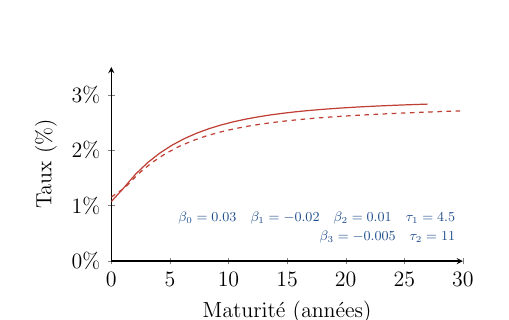
\begin{tikzpicture}[scale=0.55]
\def\MTbetaa{0.03}
\def\MTbetab{-0.02}
\def\MTbetac{0.01}
\def\MTbetad{-0.005}  % Svensson
\def\MTtaua{4.5}
\def\MTtaub{11}  % Svensson
\begin{axis}[
	width=0.8\textwidth,
	height=0.5\textwidth, 
	xlabel={Maturité (années)},ylabel={Taux (\%)},
	xmin=0, xmax=30,
	ymin=0, ymax=100*(\MTbetaa+.005),
	enlarge y limits=0.125,
	thick,
	axis x line=bottom,
	axis y line=left,
	yticklabel=\pgfmathprintnumber{\tick}\% 
	]
	\Large
	% Courbe de Nelson-Siegel
	\addplot[OrangeProfondIRA, thick, domain=0.01:27, samples=27] 
	{100*(\MTbetaa + \MTbetab * ((1 - exp(-x/\MTtaua)) / (x/\MTtaua)) + \MTbetac * (((1 - exp(-x/\MTtaua)) / (x/\MTtaua)) - exp(-x/\MTtaua)))}
	node  [pos=0.005] (M) {}
	node  [pos=0.10] (N) {}
	node  [pos=0.30] (O) {}
	node  [pos=0.75] (P) {}
	node  [pos=1] (Q) {};
	\addplot[dashed, OrangeProfondIRA, thick, domain=0.01:30, samples=27] 
	{100*(\MTbetaa + \MTbetab * ((1 - exp(-x/\MTtaua)) / (x/\MTtaua)) + \MTbetac * (((1 - exp(-x/\MTtaua)) / (x/\MTtaua)) - exp(-x/\MTtaua)) + \MTbetad * (((1 - exp(-x/\MTtaub)) / (x/\MTtaub)) - exp(-x/\MTtaub)))};
	% Affichage des paramètres
	\node[anchor=south east, text=BleuProfondIRA] at (rel axis cs:1,0.15) {\small 
		$\beta_0 = \MTbetaa$\quad
		$\beta_1 = \MTbetab$\quad
		$\beta_2 = \MTbetac$\quad
		$\tau_1 = \MTtaua$\quad			
	};	\node[anchor=south east, text=BleuProfondIRA] at (rel axis cs:1,0.05) {\small 
		$\beta_3 = \MTbetad$\quad
		$\tau_2 = \MTtaub$			
	};
	\node[xscale=0.2, yscale=-0.2, above=25pt] at (M) {\TresorerieMngt};
	\node[xscale=0.2, yscale=-0.2, above=25pt] at (N) {\familialTV};
	\node[xscale=0.2, yscale=-0.2, above=20pt] at (O) {\familialcar};
	\node[xscale=0.2, yscale=-0.2, above=20pt] at (P) {\archibuilding};
	\node[xscale=0.2, yscale=-0.2, above=20pt] at (Q) {\traintunnel};
\end{axis}
\end{tikzpicture}
\end{center}
\end{f}
\hrule

\begin{f}[Vasicek]
	
\end{f}

\begin{f}[CIR]
	
\end{f}

\begin{f}[Évaluation des obligations]
	
\end{f}

\begin{f}[Swaption]
	
\end{f}

\end{multicols}

\newpage
\begin{center}
\section*{Actuariat Vie}
    \medskip
\end{center}

\begin{multicols}{2}
	
% !TeX root = ActuarialFormSheet_MBFA-fr.tex
% !TeX spellcheck = fr_FR

\begin{f}[Notations sur les tables de survie]

L'âge $x$, $y$, $z$...    

$l_x$ est le nombre de personnes vivantes, par rapport à une cohorte initiale, à l'âge $x$

$\omega$ est l'âge limite des tables de mortalité.

$d_x=l_x-l_{x+1}$ est le nombre de personnes qui meurent entre l'âge $x$ et l'âge $x+1$.

$q_x$ est la probabilité de décès entre les âges de $x$ et l'âge $x+1$.
$$
\,q_x = d_x / l_x 
$$

$p_x$ est la probabilité que l'individu agé de $x$ survive à l'âge $x+1$.
$$
\,p_x+q_x=1 
$$

De même, 
$\,_nd_x = d_x + d_{x+1} + \cdots + d_{x+n-1} = l_x - l_{x+n}$ montre le nombre de personnes qui meurent entre l'âge $x$ et l'âge $x+n$.

$\,_nq_x$ est la probabilité de décès entre les âges de $x$ et l'âge $x+n$.

$$
\,_nq_x = {}_nd_x / l_x
$$
$\,_np_x$ est la probabilité d'une personne d'âge $x$ de survivre à l'âge $x+n$.
$$
\,_np_x = l_{x+n} / l_x 
$$


${}_{m|}q_{x}$, la probabilité que l'individu d'âge $x$ meurt dans la ${m+1}^e$ année.
$${}_{m|}q_{x}=\frac{d_{x+m}}{l_x}=\frac{l_{x+m}-l_{x+m+1}}{l_x}$$

$\,e_x$  est l'espérance de vie pour une personne encore en vie à l'âge $x$. 
C'est le nombre espéré d'anniversaires à vivre.
$$
\,e_x = \sum_{t=1}^{\infty} \ _tp_x 
$$
\end{f}
\hrule

\begin{f}[Coefficient ou commutations]


Ces coefficients ou commutations établies par des fonctions actuarielles qui dépendent d'une table de mortalité et d'un taux $i$ ($v=1/(1+i)$) pour établir la table actuarielle. 
$$
D_x=l_x .v^x
$$
peut être vu "comme" le nombre de survivants actualisés. Les sommes 

$$
N_x=\sum_{k\geq 0} D_{x+k}=\sum_{k= 0}^{\omega-x} D_{x+k}
$$

$$
S_x=\sum_{k\geq 0} N_{x+k}=\sum_{k\geq 0}(k+1). D_{x+k}
$$
seront utilisés pour simplifier les calculs.
De même
$$
C_x = d_x v^{ x+1} 
$$
peut être vu "comme" le nombre de décès  actualisés à l'âge $x$. Les sommes

$$
M_x=\sum_{k= 0}^{\omega-x} C_{x+k}
$$
$$
R_x=\sum_{k= 0}^{\omega-x} M_{x+k}
$$
seront utilisés pour simplifier les calculs.

Les  coefficients $D_x$ $N_x$ et $S_x$ seront utilisés pour les calculs sur les opérations en cas de vie et $C_x$ $M_x$ et $R_x$  pour les opérations en cas de décès.

\end{f} 
\hrule

\begin{f}[Les annuités viagères ou rentes]


\medskip
	

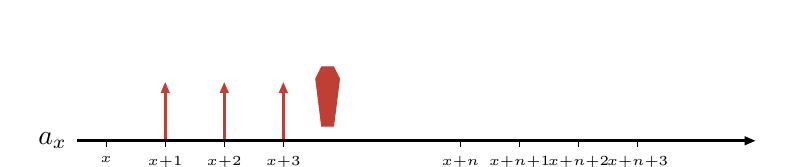
\begin{tikzpicture}[scale=0.75]
    % Draw the x-axis and y-axis.
    \def\w{11}
    \def\n{6}
    \node[left] at (-.5,0) {${}_{}a_x$};
    
    \begin{scope}[shift={(3.75,.25)}]
        \draw[color=OrangeProfondIRA,scale=0.2,fill=OrangeProfondIRA] \Cerceuil;
    \end{scope}
    \foreach \y in  {0,...,3} {
        \draw (\y,0) -- (\y,-0.1);
        \ifthenelse{\y>0 }{	\node[below] at (\y,-0.1) {\tiny $ \scriptstyle x+\y$};
            \draw[ line width=1, color=OrangeProfondIRA, arrows={-Stealth[length=4, inset=0]}] (\y,0) -- (\y,1);}{
            \node[below] at (\y,-0.1) {\tiny $ \scriptstyle x$};}
    }
    \draw (\n,0) -- (\n,-0.1);
    \node[below] at (\n,-0.1) {\tiny $\scriptstyle  x+n$};
    \foreach \y in  {1,...,3} {
        \draw (\y+\n,0) -- (\y+\n,-0.1);
        \node[below] at (\y+\n,-0.1) {\tiny $\scriptstyle x+n+\y$};
        %		\draw[ line width=1, color=OrangeProfondIRA, arrows={-Stealth[length=4, inset=0]}] (\y+\n,0) -- (\y+\n,1);
    }
    \draw[arrows={-Stealth[length=4, inset=0]}, line width=1] (-.5,0) -- (\w,0);
\end{tikzpicture}

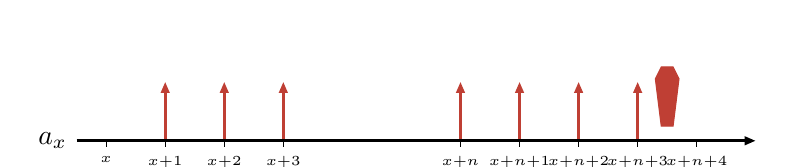
\begin{tikzpicture}[scale=0.75]
    % Draw the x-axis and y-axis.
    \def\w{11}
    \def\n{6}
    \node[left] at (-.5,0) {${}_{}a_x$};
    
    \begin{scope}[shift={(\n+.5+3,.25)}]
        \draw[color=OrangeProfondIRA,scale=0.2,fill=OrangeProfondIRA] \Cerceuil;
    \end{scope}
    \foreach \y in  {0,...,3} {
        \draw (\y,0) -- (\y,-0.1);
        \ifthenelse{\y>0 }{	\node[below] at (\y,-0.1) {\tiny $ \scriptstyle x+\y$};
            \draw[ line width=1, color=OrangeProfondIRA, arrows={-Stealth[length=4, inset=0]}] (\y,0) -- (\y,1);}{
            \node[below] at (\y,-0.1) {\tiny $ \scriptstyle x$};}
    }
    \foreach \y in  {0,...,4} {
        \draw (\y+\n,0) -- (\y+\n,-0.1);
        \ifthenelse{\y>0 }{\node[below] at (\y+\n,-0.1) {\tiny $\scriptstyle x+n+\y$};}{
            \node[below] at (\y+\n,-0.1) {\tiny $\scriptstyle x+n$};}
        \ifthenelse{\y<4 }{	\draw[ line width=1, color=OrangeProfondIRA, arrows={-Stealth[length=4, inset=0]}] (\y+\n,0) -- (\y+\n,1);}
    }
    \draw[arrows={-Stealth[length=4, inset=0]}, line width=1] (-.5,0) -- (\w,0);
\end{tikzpicture}
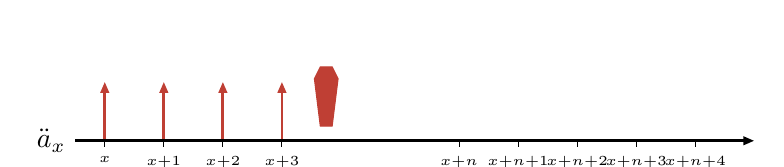
\begin{tikzpicture}[scale=0.75]
    % Draw the x-axis and y-axis.
    \def\w{11}
    \def\n{6}
    \node[left] at (-.5,0) {$\ddot{a}_x$};
    
    \begin{scope}[shift={(3.75,.25)}]
        \draw[color=OrangeProfondIRA,scale=0.2,fill=OrangeProfondIRA] \Cerceuil;
    \end{scope}
    \foreach \y in  {0,...,3} {
        \draw (\y,0) -- (\y,-0.1);
        \ifthenelse{\y>0 }{	\node[below] at (\y,-0.1) {\tiny $ \scriptstyle x+\y$};}{
            \node[below] at (\y,-0.1) {\tiny $ \scriptstyle x$};}
        \draw[ line width=1, color=OrangeProfondIRA, arrows={-Stealth[length=4, inset=0]}] (\y,0) -- (\y,1);
    }
    \draw (\n,0) -- (\n,-0.1);
    \node[below] at (\n,-0.1) {\tiny $\scriptstyle  x+n$};
    \foreach \y in  {1,...,4} {
        \draw (\y+\n,0) -- (\y+\n,-0.1);
        \node[below] at (\y+\n,-0.1) {\tiny $\scriptstyle x+n+\y$};
        %		\draw[ line width=1, color=OrangeProfondIRA, arrows={-Stealth[length=4, inset=0]}] (\y+\n,0) -- (\y+\n,1);
    }
    \draw[arrows={-Stealth[length=4, inset=0]}, line width=1] (-.5,0) -- (\w,0);
\end{tikzpicture}
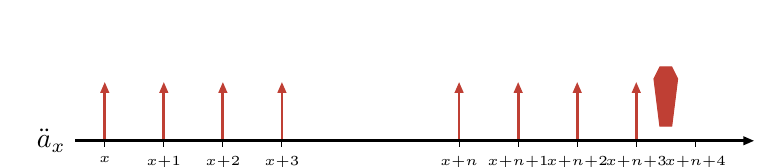
\begin{tikzpicture}[scale=0.75]
    % Draw the x-axis and y-axis.
    \def\w{11}
    \def\n{6}
    \node[left] at (-.5,0) {$\ddot{a}_x$};
    
    \begin{scope}[shift={(\n+.5+3,.25)}]
        \draw[color=OrangeProfondIRA,scale=0.2,fill=OrangeProfondIRA] \Cerceuil;
    \end{scope}
    \foreach \y in  {0,...,3} {
        \draw (\y,0) -- (\y,-0.1);
        \ifthenelse{\y>0 }{	\node[below] at (\y,-0.1) {\tiny $ \scriptstyle x+\y$};}{
            \node[below] at (\y,-0.1) {\tiny $ \scriptstyle x$};}
        \draw[ line width=1, color=OrangeProfondIRA, arrows={-Stealth[length=4, inset=0]}] (\y,0) -- (\y,1);
    }
    \foreach \y in  {0,...,4} {
        \draw (\y+\n,0) -- (\y+\n,-0.1);
        \ifthenelse{\y>0 }{\node[below] at (\y+\n,-0.1) {\tiny $\scriptstyle x+n+\y$};}{
            \node[below] at (\y+\n,-0.1) {\tiny $\scriptstyle x+n$};}
        \ifthenelse{\y<4 }{	\draw[ line width=1, color=OrangeProfondIRA, arrows={-Stealth[length=4, inset=0]}] (\y+\n,0) -- (\y+\n,1);}
    }
    \draw[arrows={-Stealth[length=4, inset=0]}, line width=1] (-.5,0) -- (\w,0);
\end{tikzpicture}	
$$a_x %=\frac{N_{x+1}}{D_x} 
%=\sum_{k=1}^{\infty}{}_{k|}q_{x} \ddot{a}_{\lcroof{k+1}}
=\sum_{k=1}^{\infty}{}_{k}p_{x} v^{k}=\ddot{a}_x -1
=\frac{N_{x+1}}{D_{x}}
$$

$$\ddot{a}_x 
%\frac{N_x}{D_x}=
%=\sum_{k=0}^{\infty}{}_{k|}q_{x} \ddot{a}_{\lcroof{k+1}}
=\sum_{k=0}^{\infty}{}_{k}p_{x} v^{k}
=	\frac{N_{x}}{D_{x}} 
$$

Si la périodicité correspond à $m$ période par an:
$$\ddot{a}_{x}^{(m)} 
=\sum_{k=0}^{\infty}\frac{1}{m}{}_{\frac{k}{m}}p_{x} v^{\frac{k}{m}}\approx\ddot{a}_x -\frac{m-1}{2m}
$$
De même, s'il paie $1/m$ en début des $m$ périodes
$$a_{x}^{(m)}\approx a_x +\frac{m-1}{2m}
$$


\textbf{Les annuités viagères temporaires} (\engl{Whole life annuity guaranteed for n years})
$$
a_{x:\lcroof{n}} =
\sum_{k=1}^{n}{}_{k}p_{x} v^{k}
=\frac{N_{x+1}-N_{x+n+1}}{D_{x}}
$$
	
$$
\ddot{a}_{x:\lcroof{n}} =%\frac{N_x - N_{x+n}}{D_x}=
\sum_{k=0}^{n-1}{}_{k}p_{x} v^{k}
=\frac{N_{x}-N_{x+n}}{D_{x}}
$$


\textbf{Les annuités viagères différées}
${}_{m|}a_{x}$ (\engl{Deferred life annuity}) représentent les rentes sur l'individu d'âge $x$ différée $m$ années. Le premier paiement intervient dans $m+1$ ans en cas de vie.

	%	\includegraphics[width=1\linewidth]{../../ActuariatVie/Graph/RenteViagereDifferee}
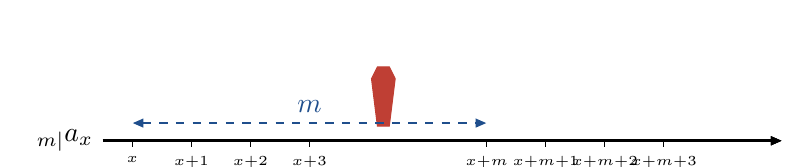
\begin{tikzpicture}[scale=0.75]
    % Draw the x-axis and y-axis.
    \def\w{11}
    \def\m{6}
    \node[left] at (-.5,0) {${}_{m|}a_x$};
    
    \begin{scope}[shift={(4.25,.25)}]
        \draw[color=OrangeProfondIRA,scale=0.2,fill=OrangeProfondIRA] \Cerceuil;
    \end{scope}
    \draw[dashed, color=BleuProfondIRA,arrows={Stealth[length=4, inset=0]-Stealth[length=4, inset=0]},  line width=1] (0,.3) -- (\m,.3) node [pos=0.5, above] {$m$};		
    \draw (0,0) -- (0,-0.1);
    \node[below] at (0,-0.1) {\tiny $x$};
    \foreach \y in  {1,...,3} {
        \draw (\y,0) -- (\y,-0.1);
        \node[below] at (\y,-0.1) {\tiny $ \scriptstyle x+\y$};
    }
    \draw (\m,0) -- (\m,-0.1);
    \node[below] at (\m,-0.1) {\tiny $\scriptstyle  x+m$};
    \foreach \y in  {1,...,3} {
        \draw (\y+\m,0) -- (\y+\m,-0.1);
        \node[below] at (\y+\m,-0.1) {\tiny $\scriptstyle x+m+\y$};
        %		\draw[ line width=1, color=OrangeProfondIRA, arrows={-Stealth[length=4, inset=0]}] (\y+\m,0) -- (\y+\m,1);
        \draw[arrows={-Stealth[length=4, inset=0]}, line width=1] (-.5,0) -- (\w,0);
    }
\end{tikzpicture}

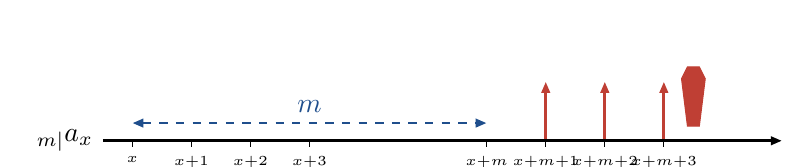
\begin{tikzpicture}[scale=0.75]
    % Draw the x-axis and y-axis.
    \def\w{11}
    \def\m{6}
    \node[left] at (-.5,0) {${}_{m|}a_x$};
    
    \begin{scope}[shift={(\m+.5+3,.25)}]
        \draw[color=OrangeProfondIRA,scale=0.2,fill=OrangeProfondIRA] \Cerceuil;
    \end{scope}
    \draw[dashed, color=BleuProfondIRA,arrows={Stealth[length=4, inset=0]-Stealth[length=4, inset=0]},  line width=1] (0,.3) -- (\m,.3) node [pos=0.5, above] {$m$};		
    \draw (0,0) -- (0,-0.1);
    \node[below] at (0,-0.1) {\tiny $x$};
    \foreach \y in  {1,...,3} {
        \draw (\y,0) -- (\y,-0.1);
        \node[below] at (\y,-0.1) {\tiny $ \scriptstyle x+\y$};
    }
    \draw (\m,0) -- (\m,-0.1);
    \node[below] at (\m,-0.1) {\tiny $\scriptstyle  x+m$};
    \foreach \y in  {1,...,3} {
        \draw (\y+\m,0) -- (\y+\m,-0.1);
        \node[below] at (\y+\m,-0.1) {\tiny $\scriptstyle x+m+\y$};
        \draw[ line width=1, color=OrangeProfondIRA, arrows={-Stealth[length=4, inset=0]}] (\y+\m,0) -- (\y+\m,1);
    }
    \draw[arrows={-Stealth[length=4, inset=0]}, line width=1] (-.5,0) -- (\w,0);
\end{tikzpicture}


  
\end{f}
\hrule

\begin{f}[Capitaux décès ou survie]

% !TeX spellcheck = fr_FR
\textbf{Les capitaux décès}(\engl{Whole life insurance } \engl{noted} ${SP}_{x}$ or ${A}_{x}$)

$A_x$ indique une prestation au décès à la fin de l'année de la mort (montant de 1), quelque que soit la date de survenance, pour un individu assuré à l'âge $x$ lors de la souscription.

$A_{x:\lcroof{n}}$ désigne un capital versé au décès s'il survient et  au plus tard dans $n$ années (\engl{Endowment}).

$\lcterm{A}{x}{n}$ % ou $\termins{x}{n}$ 
désigne un capital décès versé si $x$ décède dans les $n$ années à venir (\engl{Term insurance}).


$A_x^{(12)}$ indique une prestation   payable à la fin du mois du décès.

$\overline{A}_x$  indique une prestation  payée à la date du décès.
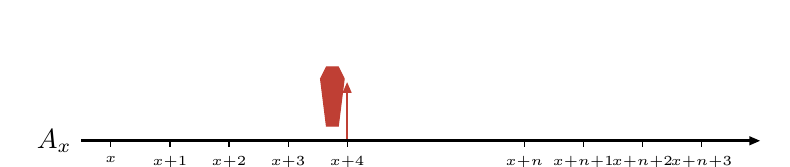
\begin{tikzpicture}[scale=0.75]
% Draw the x-axis and y-axis.
\def\w{11}
\def\n{7}
\node[left] at (-.5,0) {$A_x$};

\begin{scope}[shift={(3.75,.25)}]
    \draw[color=OrangeProfondIRA,scale=0.2,fill=OrangeProfondIRA] \Cerceuil;
\end{scope}
\draw[ line width=1, color=OrangeProfondIRA, arrows={-Stealth[length=4, inset=0]}] (4,0) -- (4,1);
\foreach \y in  {0,...,4} {
    \draw (\y,0) -- (\y,-0.1);
    \ifthenelse{\y>0 }{	\node[below] at (\y,-0.1) {\tiny $ \scriptstyle x+\y$};}{
        \node[below] at (\y,-0.1) {\tiny $ \scriptstyle x$};}
}
\draw (\n,0) -- (\n,-0.1);
\node[below] at (\n,-0.1) {\tiny $\scriptstyle  x+n$};
\foreach \y in  {1,...,3} {
    \draw (\y+\n,0) -- (\y+\n,-0.1);
    \node[below] at (\y+\n,-0.1) {\tiny $\scriptstyle x+n+\y$};
    %		\draw[ line width=1, color=OrangeProfondIRA, arrows={-Stealth[length=4, inset=0]}] (\y+\n,0) -- (\y+\n,1);
}
\draw[arrows={-Stealth[length=4, inset=0]}, line width=1] (-.5,0) -- (\w,0);
\end{tikzpicture}
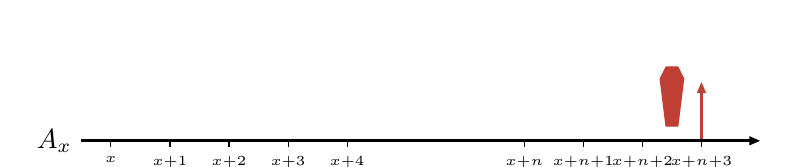
\begin{tikzpicture}[scale=0.75]
% Draw the x-axis and y-axis.
\def\w{11}
\def\n{7}
\node[left] at (-.5,0) {$A_x$};

\begin{scope}[shift={(\n+.5+2,.25)}]
    \draw[color=OrangeProfondIRA,scale=0.2,fill=OrangeProfondIRA] \Cerceuil;
\end{scope}
\draw[ line width=1, color=OrangeProfondIRA, arrows={-Stealth[length=4, inset=0]}] (\n+3,0) -- (\n+3,1);
\foreach \y in  {0,...,4} {
    \draw (\y,0) -- (\y,-0.1);
    \ifthenelse{\y>0 }{	\node[below] at (\y,-0.1) {\tiny $ \scriptstyle x+\y$};}{
        \node[below] at (\y,-0.1) {\tiny $ \scriptstyle x$};}
}
\draw (\n,0) -- (\n,-0.1);
\node[below] at (\n,-0.1) {\tiny $\scriptstyle  x+n$};
\foreach \y in  {1,...,3} {
    \draw (\y+\n,0) -- (\y+\n,-0.1);
    \node[below] at (\y+\n,-0.1) {\tiny $\scriptstyle x+n+\y$};
    %		\draw[ line width=1, color=OrangeProfondIRA, arrows={-Stealth[length=4, inset=0]}] (\y+\n,0) -- (\y+\n,1);
}
\draw[arrows={-Stealth[length=4, inset=0]}, line width=1] (-.5,0) -- (\w,0);
\end{tikzpicture}
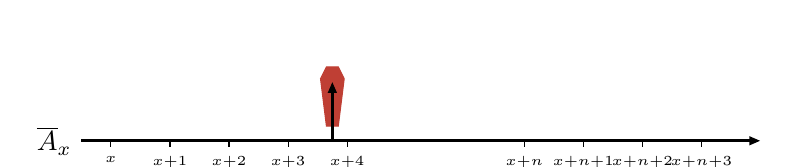
\begin{tikzpicture}[scale=0.75]
% Draw the x-axis and y-axis.
\def\w{11}
\def\n{7}
\node[left] at (-.5,0) {$\overline{A}_x$};

\begin{scope}[shift={(3.75,.25)}]
    \draw[color=OrangeProfondIRA,scale=0.2,fill=OrangeProfondIRA] \Cerceuil;
\end{scope}
\draw[ line width=1, color=black, arrows={-Stealth[length=4, inset=0]}] (3.75,0) -- (3.75,1);
\foreach \y in  {0,...,4} {
    \draw (\y,0) -- (\y,-0.1);
    \ifthenelse{\y>0 }{	\node[below] at (\y,-0.1) {\tiny $ \scriptstyle x+\y$};}{
        \node[below] at (\y,-0.1) {\tiny $ \scriptstyle x$};}
}
\draw (\n,0) -- (\n,-0.1);
\node[below] at (\n,-0.1) {\tiny $\scriptstyle  x+n$};
\foreach \y in  {1,...,3} {
    \draw (\y+\n,0) -- (\y+\n,-0.1);
    \node[below] at (\y+\n,-0.1) {\tiny $\scriptstyle x+n+\y$};
    %		\draw[ line width=1, color=OrangeProfondIRA, arrows={-Stealth[length=4, inset=0]}] (\y+\n,0) -- (\y+\n,1);
}
\draw[arrows={-Stealth[length=4, inset=0]}, line width=1] (-.5,0) -- (\w,0);
\end{tikzpicture}
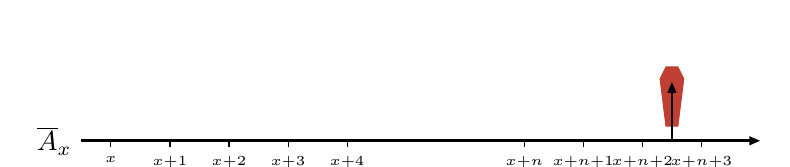
\begin{tikzpicture}[scale=0.75]
% Draw the x-axis and y-axis.
\def\w{11}
\def\n{7}
\node[left] at (-.5,0) {$\overline{A}_x$};

\begin{scope}[shift={(\n+.5+2,.25)}]
    \draw[color=OrangeProfondIRA,scale=0.2,fill=OrangeProfondIRA] \Cerceuil;
\end{scope}
\draw[ line width=1, color=black, arrows={-Stealth[length=4, inset=0]}] (\n+.5+2,0) -- (\n+.5+2,1);
\foreach \y in  {0,...,4} {
    \draw (\y,0) -- (\y,-0.1);
    \ifthenelse{\y>0 }{	\node[below] at (\y,-0.1) {\tiny $ \scriptstyle x+\y$};}{
        \node[below] at (\y,-0.1) {\tiny $ \scriptstyle x$};}
}
\draw (\n,0) -- (\n,-0.1);
\node[below] at (\n,-0.1) {\tiny $\scriptstyle  x+n$};
\foreach \y in  {1,...,3} {
    \draw (\y+\n,0) -- (\y+\n,-0.1);
    \node[below] at (\y+\n,-0.1) {\tiny $\scriptstyle x+n+\y$};
    %		\draw[ line width=1, color=OrangeProfondIRA, arrows={-Stealth[length=4, inset=0]}] (\y+\n,0) -- (\y+\n,1);
}
\draw[arrows={-Stealth[length=4, inset=0]}, line width=1] (-.5,0) -- (\w,0);
\end{tikzpicture}

\medskip

Capital décès (\engl{Whole life})
$$A_{x}=\sum_{k=0}^{\infty} {}_{k|}q_x\ \nu^{k+1}=\frac{M_x}{D_x}$$
	
$$\termins{x}{n}=\sum_{k=0}^{n-1} {}_{k|}q_x\ \nu^{k+1}=\frac{M_x-M_{x+n}}{D_x}
$$



\medskip    
\textbf{Capital différé (\engl{Pure Endowment}, capital unique en cas de survie)} noté $\lcend{A}{x}{n}$ %$\pureend{x}{n}$ 
ou ${}_n E_x$.

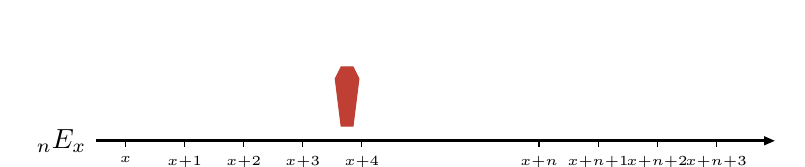
\begin{tikzpicture}[scale=0.75]
% Draw the x-axis and y-axis.
\def\w{11}
\def\n{7}
\node[left] at (-.5,0) {${}_n E_x$};

\begin{scope}[shift={(3.75,.25)}]
    \draw[color=OrangeProfondIRA,scale=0.2,fill=OrangeProfondIRA] \Cerceuil;
\end{scope}
%		\draw[ line width=1, color=OrangeProfondIRA, arrows={-Stealth[length=4, inset=0]}] (4,0) -- (4,1);
\foreach \y in  {0,...,4} {
    \draw (\y,0) -- (\y,-0.1);
    \ifthenelse{\y>0 }{	\node[below] at (\y,-0.1) {\tiny $ \scriptstyle x+\y$};}{
        \node[below] at (\y,-0.1) {\tiny $ \scriptstyle x$};}
}
\draw (\n,0) -- (\n,-0.1);
\node[below] at (\n,-0.1) {\tiny $\scriptstyle  x+n$};
\foreach \y in  {1,...,3} {
    \draw (\y+\n,0) -- (\y+\n,-0.1);
    \node[below] at (\y+\n,-0.1) {\tiny $\scriptstyle x+n+\y$};
    %		\draw[ line width=1, color=OrangeProfondIRA, arrows={-Stealth[length=4, inset=0]}] (\y+\n,0) -- (\y+\n,1);
}
\draw[arrows={-Stealth[length=4, inset=0]}, line width=1] (-.5,0) -- (\w,0);
\end{tikzpicture}
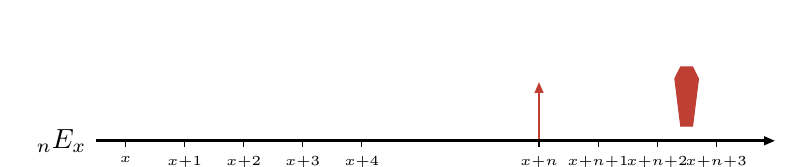
\begin{tikzpicture}[scale=0.75]
% Draw the x-axis and y-axis.
\def\w{11}
\def\n{7}
\node[left] at (-.5,0) {${}_n E_x$};

\begin{scope}[shift={(\n+.5+2,.25)}]
    \draw[color=OrangeProfondIRA,scale=0.2,fill=OrangeProfondIRA] \Cerceuil;
\end{scope}
\draw[ line width=1, color=OrangeProfondIRA, arrows={-Stealth[length=4, inset=0]}] (\n,0) -- (\n,1);
\foreach \y in  {0,...,4} {
    \draw (\y,0) -- (\y,-0.1);
    \ifthenelse{\y>0 }{	\node[below] at (\y,-0.1) {\tiny $ \scriptstyle x+\y$};}{
        \node[below] at (\y,-0.1) {\tiny $ \scriptstyle x$};}
}
\draw (\n,0) -- (\n,-0.1);
\node[below] at (\n,-0.1) {\tiny $\scriptstyle  x+n$};
\foreach \y in  {1,...,3} {
    \draw (\y+\n,0) -- (\y+\n,-0.1);
    \node[below] at (\y+\n,-0.1) {\tiny $\scriptstyle x+n+\y$};
    %		\draw[ line width=1, color=OrangeProfondIRA, arrows={-Stealth[length=4, inset=0]}] (\y+\n,0) -- (\y+\n,1);
}
\draw[arrows={-Stealth[length=4, inset=0]}, line width=1] (-.5,0) -- (\w,0);
\end{tikzpicture}
	$$
	={}_n E_x={}_n p_x .v^n=\frac{l_{x+n}}{l_x} . v^n =\frac{D_{x+n}}{D_{x}}
	$$
Capital décès avec versement du capital en cas de survie (\engl{Endowment})
$$A_{x:\lcroof{n}}=\termins{x}{n}+\lcend{A}{x}{n}$$

\end{f}
\hrule

\begin{f}[L'assurance vie sur plusieurs individus] 

$a_{xyz}$ est une rente annuelle, payée dès la fin de la première année et tant que vivent $(x)$, $(y)$ et $(z)$.

$a_{\overline{xyz}}$ est une rente annuelle, payée dès la fin de la première année et tant que vivent $(x)$, $(y)$ ou $(z)$.

$$
a_{\overline{xy}}=a_{y}+a_{x}-a_{xy}
$$

$A_{xyz}$ est une assurance qui intervient à la fin de l'année du premier décès de $(x)$, $(y)$ et $(z)$.

La barre verticale indique la conditionnalité :

$a_{x|y}$ est une rente de réversion qui profite à $(x)$ après le décès de $(y)$.

$A_{x|yz}$ est une assurance au premier décès de  $(y)$ et $(z)$.	


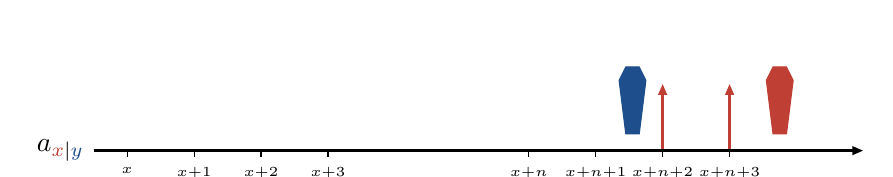
\begin{tikzpicture}[scale=0.85]
    % Draw the x-axis and y-axis.
    \def\w{11}
    \def\n{6}
    \node[left] at (-.5,0) {$a_{{\color{OrangeProfondIRA}x}|{\color{BleuProfondIRA}y}}$};
    
    \begin{scope}[shift={(9.75,.25)}]
        \draw[color=OrangeProfondIRA,scale=0.2,fill=OrangeProfondIRA] \Cerceuil;
    \end{scope}
    \begin{scope}[shift={(7.55,.25)}]
        \draw[color=BleuProfondIRA,scale=0.2,fill=BleuProfondIRA] \Cerceuil;
    \end{scope}
    \draw[ line width=1, color=OrangeProfondIRA, arrows={-Stealth[length=4, inset=0]}] (8,0) -- (8,1);
    \draw[ line width=1, color=OrangeProfondIRA, arrows={-Stealth[length=4, inset=0]}] (9,0) -- (9,1);
    \foreach \y in  {0,...,3} {
        \draw (\y,0) -- (\y,-0.1);
        \ifthenelse{\y>0 }{	\node[below] at (\y,-0.1) {\tiny $ \scriptstyle x+\y$};}{
            \node[below] at (\y,-0.1) {\tiny $ \scriptstyle x$};}
    }
    \draw (\n,0) -- (\n,-0.1);
    \node[below] at (\n,-0.1) {\tiny $\scriptstyle  x+n$};
    \foreach \y in  {1,...,3} {
        \draw (\y+\n,0) -- (\y+\n,-0.1);
        \node[below] at (\y+\n,-0.1) {\tiny $\scriptstyle x+n+\y$};
    }
    \draw[arrows={-Stealth[length=4, inset=0]}, line width=1] (-.5,0) -- (\w,0);
\end{tikzpicture}
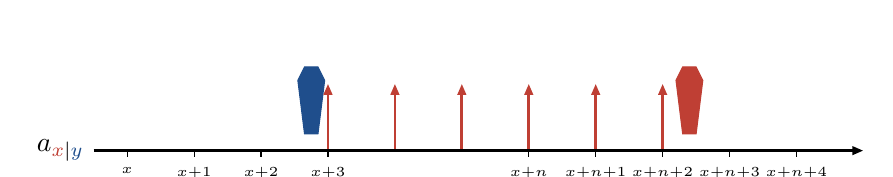
\begin{tikzpicture}[scale=0.85]
    % Draw the x-axis and y-axis.
    \def\w{11}
    \def\n{6}
    \node[left] at (-.5,0) {$a_{{\color{OrangeProfondIRA}x}|{\color{BleuProfondIRA}y}}$};
    
    \begin{scope}[shift={(8.4,.25)}]
        \draw[color=OrangeProfondIRA,scale=0.2,fill=OrangeProfondIRA] \Cerceuil;
    \end{scope}
    \begin{scope}[shift={(2.75,.25)}]
        \draw[color=BleuProfondIRA,scale=0.2,fill=BleuProfondIRA] \Cerceuil;
    \end{scope}
    \foreach \y in  {3,...,8} {
        \draw[ line width=1, color=OrangeProfondIRA, arrows={-Stealth[length=4, inset=0]}] (\y,0) -- (\y,1);
    }
    \foreach \y in  {0,...,3} {
        \draw (\y,0) -- (\y,-0.1);
        \ifthenelse{\y>0 }{	\node[below] at (\y,-0.1) {\tiny $ \scriptstyle x+\y$};}{
            \node[below] at (\y,-0.1) {\tiny $ \scriptstyle x$};}
    }
    \foreach \y in  {0,...,4} {
        \draw (\y+\n,0) -- (\y+\n,-0.1);
        \ifthenelse{\y>0 }{\node[below] at (\y+\n,-0.1) {\tiny $\scriptstyle x+n+\y$};}{
            \node[below] at (\y+\n,-0.1) {\tiny $\scriptstyle x+n$};}
    }
    \draw[arrows={-Stealth[length=4, inset=0]}, line width=1] (-.5,0) -- (\w,0);
\end{tikzpicture}
\begin{tikzpicture}[scale=0.85]
    % Draw the x-axis and y-axis.
    \def\w{11}
    \def\n{6}
    \node[left] at (-.5,0) {$a_{{\color{OrangeProfondIRA}x}|{\color{BleuProfondIRA}y}}$};
    
    \begin{scope}[shift={(3.75,.25)}]
        \draw[color=OrangeProfondIRA,scale=0.2,fill=OrangeProfondIRA] \Cerceuil;
    \end{scope}
    \begin{scope}[shift={(7.55,.25)}]
        \draw[color=BleuProfondIRA,scale=0.2,fill=BleuProfondIRA] \Cerceuil;
    \end{scope}
    \foreach \y in  {0,...,3} {
        \draw (\y,0) -- (\y,-0.1);
        \ifthenelse{\y>0 }{	\node[below] at (\y,-0.1) {\tiny $ \scriptstyle x+\y$};}{
            \node[below] at (\y,-0.1) {\tiny $ \scriptstyle x$};}
    }
    \draw (\n,0) -- (\n,-0.1);
    \node[below] at (\n,-0.1) {\tiny $\scriptstyle  x+n$};
    \foreach \y in  {1,...,4} {
        \draw (\y+\n,0) -- (\y+\n,-0.1);
        \node[below] at (\y+\n,-0.1) {\tiny $\scriptstyle x+n+\y$};
        %		\draw[ line width=1, color=OrangeProfondIRA, arrows={-Stealth[length=4, inset=0]}] (\y+\n,0) -- (\y+\n,1);
    }
    \draw[arrows={-Stealth[length=4, inset=0]}, line width=1] (-.5,0) -- (\w,0);
\end{tikzpicture}
\end{f}

\begin{f}[Schémas simplifié de tarification des primes périodiques et provisions]
	
\tikzstyle{startstop} = [rectangle, rounded corners, text width=4cm, minimum height=1cm,text centered, draw=black, fill=BleuProfondIRA!40]
\tikzstyle{process} = [rectangle, minimum width=4cm, minimum height=1cm, text centered, text width=3cm, draw=black, fill=OrangeProfondIRA!40]
\tikzstyle{arrow} = [thick,->,>=stealth]
\ \medskip

\centering
\begin{tikzpicture}[node distance=35mm and 100mm]
	\node (pu) [startstop] {Prime Unique de la prestation\\  notée $PU(.)$ ou $PV_0(.)$};
	\node  [below left of=pu, text width=55mm, node distance=18mm, xshift=12mm] {Le point est $A$ ou $a$ ou $E$ ou ...\\
	avec $x,k,n,m,K...$};
	\node (puu) [startstop, right of=pu, node distance=50mm] {Valeur d'une prime périodique unitaire\\  notée $PPU_0$ ou $VP_P$};
	\node  [below of=puu, text width=3cm, node distance=12mm] { $PPU=_{m'|}\ddot{a}_{x:\lcroof{n'}}^{(k')} $};
	\node (ppp) [startstop, below of=pu] {Prime Pure Périodique\\ $PPP$};
	\node  [below right of=ppp, text width=3cm, node distance=25mm, yshift=6mm] {$\displaystyle PPP=\frac{PU(.)}{PPU_0}$};
	\node (ppc) [startstop, right of=ppp, node distance=50mm] {Prime Périodique Chargée $PPC$};
	\node  [below of=ppc, node distance=12mm] {$\displaystyle PPC=\frac{PPP(1+\lambda)}{1-com}$};
	\node (Prov) [startstop, below of=ppp] {Provision mathématique $t^e$ année\\  notée $PM_t$ ou $V_t$ };
	\node (provt) [below right of=Prov,text width=10cm, node distance=30mm] {$V_t=PV_t(.)-PPP\times PPU_t$ \\
	$PV_t(.)$ recalculée avec  $x+t,k,n,m-t,K...\ si\ t\geq m$ \\
	ou $x+t,k,n-(t-m),m=0,K...\ si\ t>m$\\
	de même	$PPU_t=_{(m'-t)^+|}\ddot{a}_{x+t:\lcroof{n'-(t-m)^+}}^{(k')} $};
%	\node (pro2b) [startstop, right of=dec1, xshift=2cm] {Process 2b};
%	\node (stop) [startstop, below of=pro2b] {Stop};
	
	\draw [arrow] (pu) -- (ppp);
	\draw [arrow] (puu) -- (ppp);
	\draw [arrow] (ppp) -- (ppc);
	\draw [arrow] (ppp) -- node[anchor=east] {$t$} (Prov);
%	\draw [arrow] (dec1) -- node[anchor=south] {no} (pro2b);
%	\draw [arrow] (pro2b) |- (ppp);
%	\draw [arrow] (ppp) -- (stop);
	
\end{tikzpicture}
\end{f}
\end{multicols}


\newpage
\begin{center}
    \section*{Probabilités  \& Statistiques}
    \medskip
\end{center}

\begin{multicols}{2}

% !TeX root = ActuarialFormSheet_MBFA-fr.tex
% !TeX spellcheck = fr_FR

\begin{f}[Axiomatique]{\ }
	
	Un \textbf{univers} $\Omega$, est l'ensemble de tous les résultats possibles qui peuvent être obtenus au cours d'une expérience aléatoire.
	
	L'\textbf{événement aléatoire} est un événement $\omega_i$ de l'univers dont l'issue (le résultat) n'est pas certaine.
	
	
	L'\textbf{événement élémentaire :}
	\begin{itemize}
		\item deux événements élémentaires distincts $\omega_i$ et $\omega_j$ sont incompatibles,
		\item la réunion de tous les événements élémentaires de l'univers $\Omega $ correspond à la certitude.
	\end{itemize}
	
	Les \textbf{ensembles} :
	\begin{itemize}
		\item  $E=\lbrace \omega_{i1},\ldots , \omega_{ik}\rbrace$ un sous-ensemble de $\Omega$ ($k$ éléments).
		\item $\overline{E}$ le complémentaire de $E$,
		\item $E\cap F$ l'intersection de $E$ et $F$,
		\item $E\cup F$ l'union de $E$ et $F$,
		\item $E\setminus F= E\cap\overline{F}$  $E$ moins $F$,
		\item $\varnothing$ l'événement impossible ou vide.
	\end{itemize}
	
	Soit $E$ un ensemble. On appelle \textbf{tribu} ou \textbf{$\sigma-$algèbre} sur $E$, un ensemble $\mathcal{A}$ de parties de $E$ qui vérifie :
	\begin{itemize}
		\item     $\mathcal{A} \not=\varnothing$,
		\item     $\forall A \in \mathcal{A} , \overline{A} \in\mathcal{A}$,
		\item     si $\forall n \in \mathbb{N}$, $A_n \in\mathcal{A}$ alors $\cup_{n\in\mathbb{N} } A_n \in\mathcal{A}$.
	\end{itemize}
	
	On appelle \textbf{probabilité} $\mathbb{P}$ toute application de l'ensemble des évènements $\mathcal{A}$ dans l'intervalle $[0,1]$, telle que :      $$\mathbb{P} :      \mathcal{A}  \mapsto   [0,1]$$
	satisfaisant les propriétés (ou axiomes) suivantes~:
	\begin{description}
		\item[(P1)] $A \subseteq \mathcal{A} $    alors  $ \mathbb{P}(A) \geq 0$,
		\item[(P2)] $ \mathbb{P}(\Omega) = 1$,
		\item[(P3)] $A, B \subseteq \mathcal{A}$,  si  $A\cap B =\varnothing$    alors   $\mathbb{P}(A\cup B)=\mathbb{P}(A) + \mathbb{P}(B)$.
	\end{description}
	
	L'\textbf{espace de probabilité}\index{D\'efinition! espace de probabilité} se définit par 
	\[ \lbrace \Omega, \mathcal{A}, \mathbb{P}(.) \rbrace \]
	
	L'\textbf{égalité de poincarré} s'écrit~:
	$$\forall A \in F, \forall B \in F, \mathbb{P} (A \cup B) = \mathbb{P} (A) + \mathbb{P} (B) - \mathbb{P} (A \cap B)$$
	
\end{f}
\hrule

\begin{f}[Bayes]
	En théorie des probabilités, la \textbf{probabilité conditionnelle} d'un événement $A$, sachant qu'un autre événement $B$ de probabilité non nulle s'est réalisé.
	$$
	\mathbb{P}(A|B) = \frac{\mathbb{P}(A \cap B)}{\mathbb{P}(B)}
	$$
	Le réel $\mathbb{P}(A|B)$ se lit 'probabilité de $A$, sachant $B$.
	Le théorème de Bayes permet d'écrire~:
	
	$$   \mathbb{P}(A|B) = \frac{\mathbb{P}(B|A)\mathbb{P}(A)}{\mathbb{P}(B)}. $$
\end{f}
\hrule

\begin{f}[Variables aléatoires]
	
	Soient $ (\Omega, \mathcal{A}, \mathbb{P})$ un espace probabilisé. On appelle \textbf{variable aléatoire} $X$ de $\Omega$ vers $ \Re$, toute fonction mesurable $X:\Omega\mapsto \Re$.
	
	$$\lbrace X\leq x \rbrace\equiv \lbrace e\in \Omega \mid X(e)\leq x \rbrace \in   \mathcal{A}$$
	L'ensemble des événements de $\Omega$ n'est souvent pas explicite.
	
	La \textbf{fonction de répartition} $(F_X)$ d'une variable aléatoire réelle caractérise sa loi de probabilité. 
	$$
	F_X(x)=\mathbb {P}(X\leq x), x\in \Re
	$$
	où le membre de droite représente la probabilité que la variable aléatoire réelle $X$ prenne une valeur inférieure ou égale à $x$.
	La probabilité que $X$ se trouve dans l'intervalle $]a, b]$ est donc, si $a< b$,
	$
	\mathbb{P}(a< X\leq b)\ =\ F_X(b)-F_X(a)
	$
	
	Une loi de probabilité possède une \textbf{densité de probabilité} $f$, si $f$ est une fonction définie sur $\mathbb{R}^{+}$,  Lebesgue-intégrable, telle que la probabilité de l'intervalle $[a, b]$ est donnée par
	$$
	\mathbb{P}(a< X\leq b)=\int_a^b f(x) \mathrm{dx} \mbox{ pour tous nombres tq }a<x<b.
	$$
\end{f}
\hrule
\begin{f}[Espérance]{\ }
	
	L'espérance mathématique dans le cas discret (variables qualitatives ou quantitatives discrètes)~:
	$$
	\mathbb{E}[X]=\sum_{j\in \mathbb{N}}x_j\mathbb{P}(x_j)
	$$
	où $\mathbb{P}(x_j)$ est la probabilité associée à chaque événement $x_i$.
	
	L'espérance mathématique dans le cas continu~:
	$$
	\mathbb{E}[X]=\int_{-\infty}^{\infty} x. f(x)dx
	$$
	
	où $f$ désigne la fonction de densité de la variable aléatoire $x$, définie dans notre cas sur $\mathbb{R}$.
	S'agissant de somme ou d'intégrale, l'espérance est linéaire, c'est-à-dire~:
	
	$$\mathbb{E}[c_0+c_1X_1+c_2X_2]=c_0+c_1\mathbb{E}[X_1]+c_2\mathbb{E}[X_2]$$
	
	$$
	\mathbb{E}[X]=\int x.f(x)dx =\int_0^1 F^{-1}(p)dp= \int \overline{F}(x)dx\\
	$$ 
\end{f}
\hrule
\begin{f}[Convolution ou loi de la somme]{\ }
	
	La convolution de deux fonctions \( f \) et \( g \), notée \( (f * g)(x) \), est définie par :
	
	\[
	(f * g)(x) = \int f(t) g(x - t) \, dt
	\]
	
	La convolution mesure comment \( f(t) \) et \( g(t) \) interagissent à différents points tout en tenant compte du décalage (ou translation) entre 
	Si \(X\) et \(Y\) sont deux variables aléatoires indépendantes de densités respectives \(f_X\) et \(f_Y\), alors la densité de la somme \(Z = X + Y\) est donnée par :
\[
f_Z(x) = (f_X * f_Y)(x) = \int_{-\infty}^{+\infty} f_X(t)\, f_Y(x - t)\, dt.
\]

\end{f}
\hrule
\begin{f}
	[Loi composée ou modèle fréquence/gravité]{\ }
	
	Soit $N$ une variable aléatoire discrète dans $\mathbb{N}^+$, $\left(X_i\right)$ une suite de variable aléatoire $iid$ d'espérance et variance finies, alors pour  $\displaystyle S=\sum_{i=1}^{N}X_i$ :
	$$
	\mathbb{E}(S) = \mathbb{E} (\mathbb{E} [S \mid N]) = \mathbb{E} (N.\mathbb{E}(X_1)) = \mathbb{E}(N).\mathbb{E}(X_1)
	$$
	$$
	Var (S) = \mathbb{E} (Var [S \mid N]) + Var (\mathbb{E} [S \mid N])
	$$
\end{f}

\hrule
\begin{f}[Théorèmes fondamentaux] {\ }
	
	Soit $X$ une variable aléatoire réelle définie sur un espace probabilisé $\left(\Omega,\mathcal A,\mathbb P\right)$, et supposée presque sûrement positive ou nulle. L'\textbf{Inégalité de Markov} donne~:
	$$
	\forall \alpha >0, \mathbb P(X\geq \alpha)\leqslant\frac{\mathbb{E}[X]}{\alpha}.
	$$
	
	L'\textbf{inégalité de Bienaymé-Tchebychev} : 
	Pour tout réel strictement positif $\alpha$, avec $\mathbb{E}[X]=\mu$ et $\operatorname{Var}[X]=\sigma^2$
	$$
	\mathbb{P}\left(\left|X-\mu\right| \geq \alpha \right) \leq \frac{\sigma^2}{\alpha^2}.
	$$
	
	La \textbf{loi faible des grands nombres} considère une suite $(X_i)_{i\geq n\in\mathbb{N}^*}$ de variables aléatoires indépendantes définies sur un même espace probabilisé, ayant mêmes espérance et  variance finies notées respectivement $\mathbb{E}[X]$ et $\operatorname{Var}(X)$.
	
	$$
	\forall\varepsilon>0,\quad \lim_{n \to +\infty} \mathbb{P}\left(\left|\frac{X_1+X_2+\cdots+X_n}{n} - \mathbb{E}[X]\right| \geq \varepsilon\right) = 0
	$$
	
	Considérons une suite $(X_n)_{n\in \mathbb{N}}$ de variables aléatoires indépendantes qui suivent la même loi de probabilité, intégrables, i. e. $E(|X_0|)<+\infty$. 
	
	En reprenant les notations, la \textbf{loi forte des grands nombres} précise que $(Y_n)_{n\in\mathbb{N}}$ converge vers $E(X)$ \og{} presque sûrement\fg{}.
	%
	$$
	\mathbb{P}\left(\lim_{n \to +\infty} Y_n = E(X)\right)=1
	$$
	Considérons la somme $S_n = X_1 + X_2 + \cdots + X_n$.
	$$   
	Z_n\ =\ \frac{S_n - n \mu}{\sigma \sqrt{n}}\ =\ \frac{\overline{X}_n-\mu}{\sigma/\sqrt{n}},
	$$
	
	l'espérance et l'écart-type de $Z_n$ valent respectivement 0 et 1 : la variable est ainsi dite centrée et réduite.
	
	Le \textbf{théorème central limite} stipule alors que la loi de $Z_n$ converge en loi vers la loi normale centrée réduite $\mathcal{N} (0 , 1)$ lorsque $n$ tend vers l'infini. Cela signifie que si $\Phi$ est la fonction de répartition de $\mathcal{N} (0 , 1)$, alors pour tout réel $z$ :
	$$
	\lim_{n \to \infty} \mbox{P}(Z_n \le z) = \Phi(z),
	$$
	ou, de façon équivalente :
	$$
	\lim_{n\to\infty}\mbox{P}\left(\frac{\overline{X}_n-\mu}{\sigma/\sqrt{n}}\leq z\right)=\Phi(z)
	$$
\end{f}
\hrule

\begin{f}[Variables multidimensionnelles]
			
			
Une loi de probabilité est dite \textbf{multidimensionnelle}, ou $n-$dimensionnelle, lorsque la loi décrit plusieurs valeurs (aléatoires) d'un phénomène aléatoire.  
Le caractère multidimensionnel apparaît ainsi lors du transfert, par une variable aléatoire, de l'espace probabilisé $(\Omega,\mathcal{A})$ vers un espace numérique $E^n$ de dimension $n$. 

Soit une variable aléatoire $X$ sur l'espace probabilisé $(\Omega, \mathcal A, \mathbb{P})$, à valeurs dans ${\mathbb{R}}^n$ muni de la tribu borélienne réelle produit ${\mathcal {B}(\mathbb{R})}^{\otimes n}$. 
La loi de la variable aléatoire $X$ est la mesure de probabilité $\mathbb{P}_X$ définie par~:
$$
\mathbb{P}_X(B) = \mathbb{P}\big(X^{-1}(B)\big) = \mathbb{P}(X \in B).
$$
pour tout $B \in {\mathcal B(\mathbb R)}^{\otimes n}$.

Le théorème de \textbf{Cramer-Wold} assure que la loi ($n-$dimensionnelle) de ce vecteur aléatoire est entièrement déterminée par les lois (unidimensionnelles) de toutes les combinaisons linéaires de ces composantes : 
$$\sum_{i = 1}^n a_i X_i\mbox{ pour tous }a_1, a_2, \dots, a_n$$


\end{f}
\hrule

\begin{f}[Loi marginale]
La loi de probabilité de la $i^e$ coordonnée d'un vecteur aléatoire est appelée la $i^e$ loi marginale. La \textbf{loi marginale} $\mathbb{P}_i$ de $\mathbb{P}$ s'obtient par la formule :
$$
\mathbb{P}_i(B) = \mathbb{P}_{X_i}(B) = \iint { \mathds{1}}_{\omega_i\in B} \mathbb{P}(\mathrm{d}(\omega_1,\dots,\omega_n)), \forall  B \in \mathcal B(\mathbb{R}).
$$
Les lois marginales d'une loi absolument continue s'expriment à l'aide de leurs densités marginales.


La fonction de densité conditionnelle $X_2$ sachant la valeur $x_1$ de $X_1$, peut s'écrire~:
$$
f_{X_2}(x_2 \mid X_1=x_1) = \frac{f_{X_1, X_2}(x_1,x_2)}{f_{X_1}(x_1)}, 
$$

$$
f_{X_2}(x_2 \mid X_1=x_1)f_{X_1}(x_1) = f_{X_1,X_2}(x_1, x_2) = f_{X_1}(x_1 \mid X_2=x_2)f_{X_2}(x_2). 
$$
\end{f}
\hrule

	\begin{f}[Indépendance]
$(X_1, X_2, \dots,X_n)$ est une famille de \textbf{variables aléatoires indépendantes} si l'une des deux conditions suivantes est remplie :
$$
\forall (A_1,\dots,A_n)\in\mathcal{E}_1\times\dots\times\mathcal{E}_n
$$
$$
\mathbb{P}(X_1\in A_1\text{ et }X_2\in A_2\dots\text{ et }X_n\in A_n)\ =\ \prod_{i=1}^n\mathbb{P}(X_i\in A_i),
$$
on a l'égalité
$$
\mathbb{E}\left[\prod_{i=1}^n\ \varphi_i(X_i)\right]\ =\ \prod_{i=1}^n\mathbb{E}\left[\varphi_i(X_i)\right],
$$
pour n'importe quelle suite de fonctions $\varphi_i$ définies sur $(E_i,\mathcal{E}_i)$, à valeurs dans $\mathbb{R}$, dès que les espérances ci-dessus ont un sens.
$$
f_X(x)= \prod_{i=1}^{n}f_{X_i}(x_i)
$$
\end{f}
\hrule



\begin{f}[Dépendance parfaite en dimension 2]
Soient $F_1,F_2$ fonctions de répartition $\mathbb{R}\rightarrow [0,1]$.

Les \textbf{classes de Fréchet} $\mathcal{F}_{(F_1,F_2)}$ regroupent l'ensemble des fonctions de répartition $\mathbb{R}^2\rightarrow [0,1]$
dont les lois marginales sont précisément  $F_1,F_2$.
	
Pour tout $F \in \mathcal{F} (F_1,F_2)$, et pour tout $x$ in $\mathbb{R}^d$
$$
F^-(\boldsymbol{x})\leq F (\boldsymbol{x})\leq F^+(\boldsymbol{x})
$$
où $F^+(\boldsymbol{x}) = \min \{F_1(x_1),F_2(x_2)\}$, et 
$F^-(\boldsymbol{x}) = \max\{0,F_1(x_1) +F_2(x_2)-1\}$.



\begin{enumerate}
	\item Le couple $\boldsymbol{X}=(X_1,X_2)$ est dit comonotone si et seulement s'il  admet $F^+$ comme fonction de répartition.
	\item Le couple $\boldsymbol{X}=(X_1,X_2)$ est dit antimonotone si et seulement s'il  admet $F^-$ comme fonction de répartition.
\end{enumerate}

Le couple $\boldsymbol{X}=(X_1,X_2)$ est dit \textbf{comonotone} (\textbf{antimonotone}) s'il existe des fonctions non-décroissantes (non-croissante) $g_1$ et $g_2$ d'une  variable aléatoire $Z$ telles que 
$$
\boldsymbol{X}=(g_1(Z),g_2(Z))
$$
\end{f}
\hrule

\begin{f}[Le vecteur gaussien]
Un vecteur $X=(X_1,\cdots, X_n)$ est dit \textbf{vecteur gaussien}, de loi $\mathcal{N}(\boldsymbol{\mu}, \boldsymbol{\Sigma})$, lorsque toute combinaison linéaire $\sum_{j=1}^{n}\alpha_jX_j$ de ses composantes est la loi normale univariée. % (avec la convention de $\mathcal{N}(\mu, \sigma))$
En particulier, chaque composante $X_1,\cdots, X_n$ est de loi normale.
\begin{tikzpicture}[scale=0.8]
	\def\mua{2}
	\def\mub{1.5}
	\def\sigmaa{1}
	\def\sigmab{1.4}
	\begin{axis}[
		colormap name  = whitetoblue,
		width          = 9cm,
		view           = {45}{65},
		enlargelimits  = false,
		grid           = major,
		domain         = -1:4,
		y domain       = -1:4,
		samples        = 26,
		xlabel         = {$x_1$},
		ylabel         = {$x_2$},
		zlabel         = {},
		colorbar,
		colorbar style = {
			at     = {(1.1,0)},
			anchor = south west,
			height = 0.25*\pgfkeysvalueof{/pgfplots/parent axis height},
			title  = {\ \ \ \ \ \ $f_{X_1,X_2}(x_1,x_2)$}
		}
		]
		\addplot3 [surf] {Normale2(\x,\y,\mua,\sigmaa,\mub,\sigmab,-0.6)};
		\addplot3 [domain=-1:4,samples=31, samples y=0, thick, smooth]
		(\x,4,{normal(\x,\mua,\sigmaa)});
		\addplot3 [domain=-1:4,samples=31, samples y=0, thick, smooth]
		(-1,\x,{normal(\x,\mub,\sigmab)});
		%		
		\draw [black!50] (axis cs:-1,0,0) -- (axis cs:4,0,0);
		\draw [black!50] (axis cs:0,-1,0) -- (axis cs:0,4,0);
		%
		\node at (axis cs:-1,4,-0.15) [pin=165:$f_{X_1}(x_1)$] {};
		\node at (axis cs:0,4,0.1) [pin=-15:$f_{X_2}(x_2)$] {};
	\end{axis}
\end{tikzpicture}


\begin{itemize}
	\item $\boldsymbol{\mu}$ de $\mathbb{R}^N$ sa localisation,
	\item  $\boldsymbol{\Sigma}$ semi-définie positive de $\mathcal{M}_N(\mathbb{R})$, sa variance-covariance.
\end{itemize} 

Si $\boldsymbol{\Sigma}$ est bien définie positive, donc inversible, alors
% $f_{\left(\boldsymbol{\mu},\boldsymbol{\Sigma}\right)} :\mathbb{R}^N \to \mathbb{R}$ :
$$
f_{\left(\boldsymbol{\mu},\boldsymbol{\Sigma}\right)}\left(\boldsymbol{x}\right)= \frac{1} {(2\pi)^{N/2} \left| \boldsymbol{\Sigma}\right|^{1/2}}e^{ -\frac{1}{2}\left(\boldsymbol{x}-\boldsymbol{\mu}\right)^\top\boldsymbol{\Sigma}^{-1}\left(\boldsymbol{x}-\boldsymbol{\mu}\right) }.
$$
où $\left| \boldsymbol{\Sigma}\right|$ est le déterminant de $\boldsymbol{\Sigma}$.

\end{f}
\hrule

\begin{f}[Trois mesures de lien (corrélations)]

On nomme le coefficient de \textbf{corrélation linéaire de Pearson} la valeur
$$
\rho_P = \frac{\sigma_{xy}}{\sigma_x \sigma_y}
$$
où $\sigma_{xy}$ désigne la covariance entre les variables $x$ et $y$, et $\sigma_x$, $\sigma_y$ leur écart type.
$\rho$ prend ses valeurs dans $[-1,1]$ (application du théorème de Cauchy-Schwartz).

$X\bot Y \Rightarrow \rho_P=0$, Attention, $\rho_P=0 \nRightarrow X\bot Y $. 


 

Le \textbf{tau de Kendall} se définit par
$$
\tau_K=\mathbb{P}((X-X')(Y-Y')>0)-P((X-X')(Y-Y')<0)
$$
où $(X,Y)$  $(X',Y')$  sont deux couples indépendant de même densité jointe. Cela correspond à  la probabilité des concordants diminuée de celle des discordants :
\begin{align*}
\tau_K	=&\mathbb{P}\left(\operatorname{sgn}(X-X')=\mathbb{P}(\operatorname{sgn}(Y-Y')\right)-\\
		&\mathbb{P}\left(\operatorname{sgn}(X-X')\neq \operatorname{sgn}(Y-Y')\right)\\
=&\mathbb{E}\left[ \operatorname{sgn}(X-X')\operatorname{sgn}(Y-Y')\right]\\
=&\operatorname{Cov}(\operatorname{sgn}(X-X'),\operatorname{sgn}(Y-Y'))\\
=&4\mathbb{P}(X<X',Y<Y')-1 
\end{align*}

Le coefficient de corrélation \textbf{rho de Spearman} de $(X,Y)$ est défini comme le coefficient de corrélation de Pearson des rangs des variables aléatoires $X$ et $Y$.
Pour un échantillon $n$, les $n$ valeurs $X_i$, $Y_i$ sont converties par leurs rangs $x_i$, $y_i$, et $\rho$ est calculé~:
$$
\rho_S = \frac{1/n\,\sum_i(x_i-\mathbb{E}[x])(y_i-\mathbb{E}[y])}{\sqrt{1/n\,\sum_i (x_i-\mathbb{E}[x])^2 \times 1/n\sum_i(y_i-\mathbb{E}[y])^2}}.
$$
Si on note $x_i= R(X_i)$ de 1 à $N$ et  $d_i = x_i - y_i$~:
$$    \rho_S = 1- {\frac {6 \sum_i d_i^2}{n(n^2 - 1)}}$$

\end{f}
\hrule

\begin{f}[Copule]
Une \textbf{copule} est une fonction de répartition, notée $\mathcal{C}$, définie sur $[0,1]^d$ dont les marges sont uniformes sur $[0,1]$. 
Une caractérisation est alors que $\mathcal{C}(u_1,...,u_d)=0$ si une des composantes $u_i$ est nulle, $\mathcal{C}(1,...,1,u_i,1,...,1)=u_i$, et $\mathcal{C}$ est $d-$croissante.
\medskip
		
Soit $F^{(d)}$ une fonction de répartition en dimension $d$  où les $F_i$ sont les lois marginales de $F$. 

Le\textbf{ théorème de Sklar} indique que $F^{(d)}$ admet une représentation copule~:
$$
F^{(d)} (x_1,...,x_d) = \mathcal{C} (F_1(x_1),...,F_d(x_d))
$$
Si ces lois marginales sont toutes continues, la copule $\mathcal{C}$ est alors unique, et donnée par la relation 
$$
\mathcal{C}(u_1,...,u_d)=F^{(d)}(F_1^{-1} (u_1),...,F_d^{-1} (u_d))
$$
Dans ce cas, on pourra alors parler de la copule associée à un vecteur aléatoire $(X_1,...,X_d)$.	
Ce théorème est très important puisque nous pouvons séparer la partie marge de distribution de la partie dépendance. 
\medskip
	
La \textbf{Copule Gaussienne} est une distribution sur le cube unitaire de dimension $d$, $[0,1]^d$. 
Elle est construite sur la base d'une loi normale de dimension $d$ sur  $\mathbb{R}^d$.

Soit la matrice de corrélation  $\Sigma\in\mathbb{R}^{d\times d}$, la copule Gaussienne de paramètre  $\Sigma$ peut s'écrire~:
$$
\mathcal{C}_\Sigma^{Gauss}(u) = \Phi_\Sigma\left(\Phi^{-1}(u_1),\dots, \Phi^{-1}(u_d) \right), 
$$
où $\Phi^{-1}$ est la fonction de répartition inverse de la loi normale standard et  $\Phi_\Sigma$ est la distribution jointe d'une loi normale de dimension $d$, de moyenne nulle et de matrice de covariance égale à la matrice de corrélation  $\Sigma$.
\medskip	

	Une copule $\mathcal{C}$ est qualifiée d'\textbf{archimédienne} si elle admet la représentation suivante~:
$$
\mathcal{C}(u_1,\dots,u_d) = \psi^{-1}\left(\psi(u_1)+\dots+\psi(u_d)\right)\,
$$
où $\psi$ est alors appelé \textbf{générateur}.

Souvent, les copules  admettent une formulation explicite de  $\mathcal{C}$. 
Un seul paramètre permet d'accentuer la dépendance de toute la copule, quelque soit sa dimension $d$.


Cette formule fournit une copule si et seulement si $\psi\,$ est $d$-monotone sur $[0,\infty)$ \emph{i.e.} la dérivé $k^e$  de $\psi\,$ satisfait
$$
(-1)^k\psi^{(k)}(x) \geq 0
$$
pour tout $x\geq 0$ et $k=0,1,\dots,d-2$ et $(-1)^{d-2}\psi^{d-2}(x)$ est non-croissante et convexe.
\medskip

Les générateurs suivants sont tous monotones, i.e. $d$-monotone pour tout $d\in\mathbb{N}$.

\footnotesize
\renewcommand\arraystretch{1.3}
\begin{tabular}{|m{10mm}|ccc|}	\rowcolor{BleuProfondIRA!40} 
	\hline
 Nom 		& Générateur $\psi^{-1}(t)$, 	& $\psi(t)$ &	Paramètre\\
	\hline
	Ali-Mikhail-Haq 	&$\frac{1-\theta}{\exp(t)-\theta} $	
	&$\log\left(\frac{1-\theta+\theta t}{t}\right)$ 	
	&$\theta\in[0,1)$\\
	Clayton		&$\left(1+\theta t\right)^{-1/\theta} 	$
	&$\frac1\theta\,(t^{-\theta}-1)\, 	$
	&$\theta\in(0,\infty)$\\
	Frank 		&$-\frac{1}{\theta}\exp(-t)$
	&$-\log\left(\frac{\exp(-\theta t)-1}{\exp(-\theta)-1}\right)$
	&$\theta\in(0,\infty)$\\
	&$\times\log(1-(1-\exp(-\theta)))$
	&
	&\\
	Gumbel 		&$\exp\left(-t^{1/\theta}\right) $	
	&$\left(-\log(t)\right)^\theta$	
	&$\theta\in[1,\infty)$\\
	$\perp$ 	&$\exp(-t)\,$
	&$-\log(t)\,$ 	
	& \\
	Joe		&$1-\left(1-\exp(-t)\right)^{1/\theta}$
	&$-\log\left(1-(1-t)^\theta\right)$
	&$\theta\in[1,\infty)$\\
	\hline
\end{tabular}
\renewcommand\arraystretch{1}
\end{f}
\hrule

\begin{f}[Mouvement brownien, filtration et martingales]
	
Une \textbf{filtration} $(\mathcal{F}_t)_{t \geq 0}$ est une famille croissante de $\sigma$-algèbres ou tribu représentant l’information disponible jusqu’au temps $t$. Un processus $(X_t)$ est dit \textbf{$\mathcal{F}_t$-adapté} si $X_t$ est mesurable par rapport à $\mathcal{F}_t$ pour tout $t$.
	
Un processus $(B_t)_{t \geq 0}$ est un \textbf{mouvement brownien standard} (ou processus de Wiener) s’il vérifie :
	\begin{itemize} 
		\item $B_0 = 0$ ;
		\item accroissements indépendants : $B_t - B_s$  indépendant de $\mathcal{F}_s$ ;
		\item accroissements stationnaires : $B_t - B_s \sim \mathcal{N}(0, t - s)$ ;
		\item trajectoires continues presque sûrement.
	\end{itemize}
	
	Un processus $(M_t)$ est une \textbf{martingale} (par rapport à $\mathcal{F}_t$) si :
	\[
	\mathbb{E}[|M_t|] < \infty \quad \text{et} \quad \mathbb{E}[M_t \mid \mathcal{F}_s] = M_s \quad \forall\, 0 \leq s < t
	\]
	Exemples : le mouvement brownien, les intégrales stochastiques de la forme $\int_0^t \theta_s dB_s$ (sous conditions) sont des martingales.
	\medskip
	
	\textbf{Variation quadratique} est noté $
	\langle B \rangle_t = t, \quad \langle cB \rangle_t = c^2 t$
	
\textbf{Covariation} : pour deux processus d’Itô $X, Y$,
\[
\langle X, Y \rangle_t := \lim_{\|\Pi\| \to 0} \sum_{i} (X_{t_{i+1}} - X_{t_i})(Y_{t_{i+1}} - Y_{t_i})
\]
convergence en probabilité, où $\Pi = \{t_0 = 0 < t_1 < \dots < t_n = t\}$ est une partition de $[0,t]$.
\end{f}


\begin{f}[Processus d'Itô et calcul différentiel stochastique]
	
Un processus $(X_t)$ est un \textbf{processus d’Itô} s’il peut s’écrire :
	\[
	X_t = X_0 + \int_0^t \phi_s\, ds + \int_0^t \theta_s\, dB_s
	\]
	ou en différentielle
	\[dX_t = \phi_t dt + \theta_t dB_t\]
	avec $\phi_t$, $\theta_t$ $\mathcal{F}_t$-adaptés et $L^2$-intégrables.
	
	\textbf{Formule d’Itô (1D)} : pour $f \in C^2(\mathbb{R})$, on a :
	\[
	df(X_t) = f'(X_t) dX_t + \frac{1}{2} f''(X_t) d\langle X \rangle_t
	\]
	
	Exemple : si $dX_t = \mu dt + \sigma dB_t$ alors :
	\[
	dX_t^2 = 2X_t dX_t + d\langle X \rangle_t
	\]
	
	\textbf{Formule d’Itô (multi-dimension)} :\\
	Si $X = (X^1, \dots, X^d)$ est un processus d’Itô, $f \in C^2(\mathbb{R}^d)$ :
	\[
	df(X_t) = \sum_i \frac{\partial f}{\partial x_i}(X_t) dX^i_t
	+ \frac{1}{2} \sum_{i,j} \frac{\partial^2 f}{\partial x_i \partial x_j}(X_t) d\langle X^i, X^j \rangle_t
	\]
	
	\textbf{Intégration par parties (Itô)} :
	\[
	d(X_t Y_t) = X_t dY_t + Y_t dX_t + d\langle X, Y \rangle_t
	\]
	
\end{f}

\begin{f}[Équations différentielles stochastiques (EDS)]
	
	Une EDS (\emph{SDE}) est une équation stochastique de la forme :
	\[
	dX_t = b(t, X_t) dt + a(t, X_t) dB_t, \quad X_0 = x
	\]
	où :
	\begin{itemize}
		\item $b(t,x)$ est la \textbf{dérive} (\emph{drift}) : fonction $\mathbb{R}_+ \times \mathbb{R} \to \mathbb{R}$ ;
		\item $a(t,x)$ est la \textbf{diffusion} : fonction $\mathbb{R}_+ \times \mathbb{R} \to \mathbb{R}$ ;
		\item $B_t$ est un mouvement brownien ;
		\item $X_t$ est la solution, processus stochastique adapté.
	\end{itemize}
	
	\textbf{Forme intégrale} :
	\[
	X_t = x + \int_0^t b(s, X_s) ds + \int_0^t a(s, X_s) dB_s
	\]
	
	\textbf{Conditions d’existence et d’unicité} :
	\begin{itemize}
		\item \textbf{Lipschitz} : il existe $L > 0$ tel que :
		\[
		|b(t,x) - b(t,y)| + |a(t,x) - a(t,y)| \leq L |x - y|
		\]
		\item \textbf{Croissance linéaire} :
		\[
		|b(t,x)|^2 + |a(t,x)|^2 \leq C(1 + |x|^2)
		\]
	\end{itemize}
	
Exemples classique :
	\begin{itemize}
		\item \textbf{Brownien géométrique} : $dS_t = \mu S_t dt + \sigma S_t dB_t$
		\item \textbf{Ornstein–Uhlenbeck} : $dX_t = \theta(\mu - X_t) dt + \sigma dB_t$
	\end{itemize}
	
	\textbf{Méthodes numériques} : Euler–Maruyama, Milstein.
	
\end{f}

\begin{f}[Probabilité risque neutre]
	
	Une probabilité $\mathbb{Q}$ est dite \textbf{risque neutre} si, sous $\mathbb{Q}$, 
	tout actif  $S_t$ a un prix actualisé $ \frac{S_t}{B_t}$ qui est une martingale
	où $(B_t)$ est le numéraire (par exemple $B_t = e^{rt}$).
	
	L'absence d'arbitrage $\iff \exists\, \mathbb{Q} \sim \mathbb{P}$ telle que les prix actualisés soient des martingales.
	C’est le \textbf{théorème fondamental de l’évaluation des actifs}.
	
	\textbf{Application} :\\
	Sous $\mathbb{Q}$, la valeur à l’instant $t$ d’un actif donnant un retour $H$ à la date $T$ est :
	\[
	S_t = B_t\, \mathbb{E}^\mathbb{Q} \left[ \left. \frac{H}{B_T} \right\|  \mathcal{F}_t \right]
	\]
	
	\textbf{Remarque} :\\
	La mesure $\mathbb{Q}$ est équivalente à $\mathbb{P}$, mais reflète un monde "sans préférence pour le risque", utile en valorisation.
	
\end{f}
\newcolumn

%
%\begin{f}[Processus stochastiques en actuariat]
%	
%	\textbf{Brownien standard} $W_t$ :
%	\begin{itemize}
%		\item $W_0 = 0$ a.s.
%		\item $W_t$ est à accroissements indépendants et stationnaires
%		\item $W_t - W_s \sim \mathcal{N}(0, t-s)$ pour $t > s$
%		\item Trajectoires continues presque sûrement
%	\end{itemize}
%	
%	\textbf{Martingale} :
%	Un processus $(M_t)_{t \geq 0}$ adapté à une filtration $(\mathcal{F}_t)$ est une \textit{martingale} si :
%	\[
%	\mathbb{E}[|M_t|] < \infty \quad \text{et} \quad \mathbb{E}[M_t \mid \mathcal{F}_s] = M_s \quad \forall s < t
%	\]
%	
%	\textbf{Lemme d’Itô (dimension 1)} :\\
%	Soit $X_t$ une EDS : $\mathrm{d}X_t = \mu_t \,\mathrm{d}t + \sigma_t \,\mathrm{d}W_t$,\\
%	et $f : \mathbb{R} \to \mathbb{R}$ de classe $C^2$, alors :
%	\[
%	\mathrm{d}f(X_t) = f'(X_t) \,\mathrm{d}X_t + \frac{1}{2} f''(X_t) \,\sigma_t^2 \,\mathrm{d}t
%	\]
%	
%	\textbf{Équation différentielle stochastique (EDS)} :
%	\[
%	\mathrm{d}X_t = \mu(X_t, t)\,\mathrm{d}t + \sigma(X_t, t)\,\mathrm{d}W_t
%	\]
%	
%	\textbf{Exemple classique : processus de Black-Scholes} :
%	\[
%	\mathrm{d}S_t = \mu S_t\,\mathrm{d}t + \sigma S_t\,\mathrm{d}W_t
%	\quad \Rightarrow \quad
%	S_t = S_0 \exp\left((\mu - \frac{\sigma^2}{2})t + \sigma W_t\right)
%	\]
%	
%	\textbf{Mouvement brownien géométrique} :
%	\[
%	S_t = S_0 \exp(X_t), \quad \text{où } X_t = (\mu - \frac{\sigma^2}{2})t + \sigma W_t
%	\]
%	
%	\textbf{Lien avec Bachelier (1900)} :
%	Premier modèle de prix avec mouvement brownien additif :
%	\[
%	S_t = S_0 + \mu t + \sigma W_t
%	\quad \text{(modèle abandonné à cause de } S_t < 0 \text{ possible)}
%	\]
%	
%	\textbf{Lien avec Norbert Wiener} :\\
%	Formalisation rigoureuse du mouvement brownien comme processus stochastique à temps continu.
%	
%\end{f}
%\hrule

\begin{f}[Les simulations]
	\tikz{
		\def\m{2};
		\def\s{1};
	}
	%
	
	Les simulations permettent en particulier d'approximer l'espérance par la moyenne empirique des réalisations $x_1,\ldots,x_n$:
	$$
	\frac{1}{n}(x_1+\ldots+x_n)\approx \int xdF(x)=\mathbb{E}[X]
	$$
	Ensuite, en vertu du TLC, nous estimons l'incertitude ou intervalle de confiance sur la base de la loi normale:
	$$
	\left[\overline{x}-1,96\frac{S_n}{\sqrt{n}},\overline{x}+1,96\frac{S_n}{\sqrt{n}}\right]
	$$
	où $S_n$ estime sans biais la variance de $X$~:
	$$
	S_n^2=\frac{1}{n-1}\sum_{i=1}^{n}(x_i-\overline{x})^2
	$$
	
	la convergence est dite en $\mathcal{O}(\frac{\sigma}{\sqrt{n}})$. 	
	Cet intervalle permet de décider le nombre de simulations à réaliser.
\end{f}

\begin{f}[Générateur pseudo aléatoire sur ${[}0,1{]}^d$]
L'ordinateur ne sait pas lancer le dé ($\Omega=\{ \epsdice{1}, \epsdice{2}, \epsdice{3}, \epsdice{4}, \epsdice{5}, \epsdice{6} \}$).
Il génère un pseudo aléa, c'est à dire un algorithme déterministe qui ressemble à un événement aléatoire.
Les générateurs produisent généralement un aléa sur $[0,1]^d$.
Si la valeur initiale (\emph{seed}) est définie ou identifiée, les tirages suivants sont connus et répliquables.


L'algorithme le plus simple est  appelée méthode des congruences linéaires :
$$
x_{n+1}=\Phi(x_n)= (a\times x_n+c) \mod m
$$ \small
chaque $x_n$ est un entier compris entre 0 et $m-1$.
$a$ le multiplicateur [\emph{multiplier}], $c$ l'accroissement [\emph{increment}], et $m$ le modulo [\emph{modulus}] de la forme $2^p-1$, c'est-à-dire un nombre premier de Mersenne ( $ p $ nécessairement premier) :

Générateur de Marsaglia: $a=69069, b=0, m=2^{32}$

Générateur Knuth\&Lewis: $a=1664525, b=1013904223, m=2^{32}$

Générateur de Haynes: $a=6364136223846793005, b=0, m=2^{64}$

%Le générateur de Tausworthe est une extension du générateur congruentiel linéaire qui consiste à ne  plus utiliser seulement $x_{╔n-1}$ pour fabriquer un nouvel élément mais plutôt un ensemble de valeurs précédentes
Le générateur de Tausworthe, constitue une extension 'autorégressive' :
$$
x_{n}=(a_{1}\times x_{n-1}+a_{2}\times x_{n-2}+\cdots +a_{k}\times x_{n-k}) \mod m \text{ avec } n\geq k
$$
La période du générateur est $m^k-1$, avec tous les $a_i$ premiers entre eux. Si $m$ est de la forme $2^p$ , les temps de calculs machine sont réduits. 


Le générateur aléatoire par défaut est généralement l'algorithme de Mersenne-Twister. Il est basé sur une récurrence linéaire sur une matrice $F_{2}$ (matrice dont les valeurs sont en base 2, i.e. 0 ou 1). 
Son nom provient du fait que la longueur de la période choisie pour être un nombre premier de Mersenne. 
\begin{enumerate}
	\item     sa période est de $2^{19937}-1 $
	\item     il est uniformément distribué sur un grand nombre de dimensions (623 pour les nombres de 32 bits) ;
	\item     il est plus rapide que la plupart des autres générateurs ,
	\item     il est aléatoire quel que soit le poids du bit considéré, et passe les tests Diehard.
\end{enumerate}
\end{f}
%

\begin{f}[Simuler une variable aléatoire]
	
Simuler $X$ d'une loi quelconque $F_X$ revient souvent à simuler $\left(p_i\right)_{i\in [1,n]}$ de loi $\mathcal{U}ni(0,1)$.

\textbf{ Si $F_X$ est inversible},  $x_i=F^{-1}_X(p_i)$ (ou fonction quantile) livre $\left(x_i\right)_{i\in [1,n]}$ un jeu de $n$ simulations de loi $F_X$.
			
	\begin{center}
		%\tikzmath{
			%	\m = 2; 
			%	\s = 1;
			%}	
		
		\begin{tikzpicture}[xscale=.8,yscale=2]
			
			% define normal distribution function 'normaltwo'
			%	\def\normaltwo{\x,{4*1/exp(((\x-3)^2)/2)}}
			
			% input y parameter
			\def\z{3.5}
			\def\m{2};
			\def\s{1};
			
			% this line calculates f(y)
			\def\fz{normcdf(\z,\m, \s)}
			
			
			\draw[color=blue] plot [domain=-1:6] ({\x}, {normcdf(\x,\m, \s)})
			node[right] {\color{blue} $F_X(x)$};;
			
			% Add dashed line dropping down from normal.
			\draw[dashed] (0,{\fz}) node[left] {$p_i$};
			\draw[dashed,->]   (0,{\fz}) -- ({\z},{\fz}) -- ({\z},0) node[below] {$x_i=F^{-1}(p_i)$};
			
			% Optional: Add axis labels 
			\draw (6,0) node[below] {$x$};
			
			% Optional: Add axes
			\draw[->] (-1.2,0) -- (6.2,0) node[right] {};
			\draw[->] (0,0) -- (0,1.2) node[above] {};
			
		\end{tikzpicture}
	\end{center}	
	
Si c'est une variable discrète ($F^{-1}$ n'existe pas) $X_\ell=\min_{\ell} F(X_\ell)> p_i$, où $ \left(X_{\ell}\right)_{\ell}$ l'ensemble dénombrable des valeurs possibles, ordonnées de manière croissante.

Dans la méthode du \textbf{changement de variable}, on suppose qu'on sait simuler une loi $X$, et qu'il existe $\phi$ tel que $Y=\varphi(X)$ suit une loi $F_Y$. L'exemple naturelle est celui de $X\sim \mathcal{N}(0,1)$ et de faire le changement $Y=\exp(X)$ pour obtenir Y qui suit une loi lognormale.

\textbf{La méthode du rejet} est utilisée dans des cas plus complexe, par exemple lorsque $F^{-1}$ n'est pas explicite ou exige beaucoup de temps de calcul. 
Soit $f$ une fonction de densité de probabilités. On suppose qu'il existe une densité de probabilités $g$ telle que :
$$
{\displaystyle \exists K>0\ ,\ \forall x\in \mathbb {R} \ ,\ f(x)\leq Kg(x)}
$$
On simule alors $Z$ suivant la loi de densité $g$, et ${\displaystyle Y\sim {\mathcal {U}}([0;Kg(Z)])} $.
Alors la variable aléatoire ${\displaystyle X=\lbrace Z|Y\leq f(Z)\rbrace } $ suit la loi de densité $f$.



\begin{tikzpicture}[domain=-4:10,scale=0.6]
	%   \draw[very thin,color=gray] (-0.1,-1.1) grid (3.9,3.9);
	\draw[->] (-4.2,0) -- (10.2,0) node[right] {$x$};
	\draw[->] (0,0) -- (0,6) node[above] {$f(x)$};
	\draw[BleuProfondIRA] (-4,0) -- (-4,6) ;
	\draw[BleuProfondIRA] (10,0) -- (10,6) ;
	\draw[name path=melange,color=OrangeProfondIRA,smooth] plot ({\x},{20*normal(\x,2,2)+10*normal(\x,6,1)}) node[below=.5,left] {$f(x)$ , mélange loi normale};
	\draw[name path=g,color=BleuProfondIRA,smooth] plot  ({\x},{60*normal(\x,3,3)})   node[above=3.5,left] {$K\times g(x)$, densité de  loi normale };

	\tikzfillbetween[of=melange and g,on layer=main]{BleuProfondIRA, opacity=0.1};
\end{tikzpicture}

La performance de l'algorithme dépend du nombre de rejet, représenté par la surface bleu sur le graphique.
\end{f}
\hrule

%

\begin{f}[Méthodes de Monte Carlo]

Les \textbf{méthodes de Monte Carlo} reposent sur la simulation répétée de variables aléatoires pour approximer des quantités numériques.

\textbf{Convergence} :
\begin{itemize}[nosep]
	\item Par la \textbf{loi des grands nombres}, l’estimateur converge presque sûrement vers la valeur attendue.
	\item Par le \textbf{théorème central limite}, l’erreur standard est en $\mathcal{O}(N^{-1/2})$ :
	\[
	\sqrt{N}(\hat{\mu}_N - \mu) \xrightarrow{d} \mathcal{N}(0, \sigma^2)
	\]
	\item Cette convergence lente justifie l’usage de techniques d’\textbf{amélioration de la convergence}.
\end{itemize}

\textbf{Techniques de réduction de variance} :
\begin{itemize}
	\item \textbf{Variables antithétiques} : on simule $X$ et $-X$ (ou $1-U$ si $U \sim \mathcal{U}[0,1]$), puis on moyenne les résultats. Réduction efficace si $f$ est monotone.
	\item \textbf{Méthode de contrôle} : si $\mathbb{E}[Y]$ est connue, on simule $(f(X), Y)$ et on corrige :
	\[
	\hat{\mu}_\text{corr} = \hat{\mu} - \beta(\bar{Y} - \mathbb{E}[Y])
	\]
	où $\beta$ optimal minimise la variance.
	\item \textbf{Stratification} : on divise l’espace des simulations en strates (sous-ensembles), et on simule proportionnellement dans chaque strate.
	\item \textbf{Importance sampling} : on modifie la loi de simulation pour accentuer les événements rares, puis on repondère :
	\[
	\mathbb{E}[f(X)] = \mathbb{E}^{Q}\left[f(X) \frac{\mathrm{d}P}{\mathrm{d}Q}(X)\right]
	\]
	utilisée notamment pour estimer les queues de distribution (VaR, TVaR).
\end{itemize}

\end{f}
\begin{f}[Le bootstrap]
	
	Le \textbf{bootstrap} est une méthode de \textit{rééchantillonnage} permettant d’estimer l’incertitude d’un estimateur sans supposer de forme paramétrique pour la loi sous-jacente.
	
	Soit un échantillon $\xi = (X_1, X_2, \ldots, X_n)$ de variables iid suivant une loi inconnue $F$. On cherche à estimer une statistique $\theta = T(F)$ (ex. moyenne, médiane, variance), via son estimateur empirique $\hat{\theta} = T(\hat{F}_n)$.
	
	\begin{enumerate}
		\item On approxime $F$ par la fonction de répartition empirique :
		\[
		\hat{F}_n(x) = \frac{1}{n} \sum_{k=1}^n \mathbf{1}_{\{X_k \le x\}}
		\]
		
		\item On génère $B$ échantillons bootstrap $\xi^{\ast(b)} = (X_1^{\ast(b)}, \ldots, X_n^{\ast(b)})$ en tirant \textbf{avec remise} dans l’échantillon initial.
		
		\item Pour chaque échantillon simulé, on calcule l’estimation $T^{\ast(b)} = T(\hat{F}_n^{\ast(b)})$.
	\end{enumerate}
	
	Les réalisations $T^{\ast(1)}, \ldots, T^{\ast(B)}$ forment une approximation de la distribution de l’estimateur $\hat{\theta}$.
	
	On peut en déduire :
	\begin{itemize}[nosep]
		\item un \textbf{biais estimé} : $\widehat{\text{bias}} = \overline{T^\ast} - \hat{\theta}$ ;
		\item un \textbf{intervalle de confiance} à $(1-\alpha)$ : $[q_{\alpha/2},\ q_{1 - \alpha/2}]$ des quantiles empiriques de $T^{\ast(b)}$ ;
		\item une estimation de la \textbf{variance} : $\widehat{\mathrm{Var}}(T^\ast)$.
	\end{itemize}
	
	\textbf{Remarque} : Le bootstrap est particulièrement utile lorsque la distribution de $T$ est inconnue ou difficile à estimer analytiquement.
	
\end{f}
\begin{f}[Bootstrap paramétrique]
	
	Le \textbf{bootstrap paramétrique} repose sur l’hypothèse que les données suivent une famille de lois paramétrée $\{F_\theta\}$.
	
	Soit $\xi = (X_1, \ldots, X_n)$ un échantillon $iid$ selon une loi $F_\theta$ inconnue. On procède comme suit :
	\begin{enumerate}
		\item Estimer le paramètre $\hat{\theta}$ à partir de $\xi$ (ex. par maximum de vraisemblance).
		\item Générer $B$ échantillons $\xi^{\ast(b)}$ de taille $n$, simulés selon la loi $F_{\hat{\theta}}$.
		\item Calculer $T^{\ast(b)} = T(\xi^{\ast(b)})$ pour chaque échantillon.
	\end{enumerate}
	
	Ce procédé approxime la distribution de l’estimateur $T(\xi)$ en supposant connue la forme de $F$. Il est plus efficace que le bootstrap non paramétrique si l’hypothèse de modèle est bien spécifiée. Le bootstrap paramétrique est plus rapide, mais hérite des biais du modèle.
	
\end{f}

\begin{f}[Validation croisée]
	
	La \textbf{validation croisée} est une méthode d’évaluation de la performance prédictive d’un modèle statistique, utilisée notamment en machine learning ou en tarification.
	
	\textbf{Principe} :
	\begin{itemize}
		\item Diviser les données en $K$ blocs (ou folds).
		\item Pour chaque $k = 1,\ldots,K$ :
		\begin{itemize}
			\item Entraîner le modèle sur les $K-1$ autres blocs.
			\item Évaluer la performance (erreur, log-vraisemblance...) sur le $k$-ième bloc.
		\end{itemize}
		\item Agréger les erreurs pour obtenir une estimation globale de la performance hors-échantillon.
	\end{itemize}
	
\end{f}

%
\begin{f}[Méthodes quasi-Monte Carlo]
	
	Les méthodes \textbf{quasi-Monte Carlo} visent à \textbf{accélérer la convergence} de l’estimateur d’espérance sans recourir à l’aléatoire. L’erreur typique est de l’ordre :
	\[
	\mathcal{O}\left( \frac{(\ln N)^s}{N} \right)
	\]
	où $N$ est la taille de l’échantillon et $s$ la dimension du problème.
	
	Ces méthodes reposent sur l’utilisation de suites \textbf{à discrépance faible} dans $[0,1]^s$. La discrépance à l'origine (\emph{star discrepancy}), notée  $D^*_N(P)$ pour un ensemble de points $P = \{x_1, \ldots, x_N\}$, mesure l’écart maximal entre la proportion de points contenus dans des rectangles \emph{ancrés à l’origine} et leur volume. Elle est définie par :
	\[
	D^*_N(P) = \sup_{u \in [0,1]^s} \left| \frac{1}{N} \sum_{i=1}^N \mathbf{1}_{[0,u)}(x_i) - \lambda_s([0,u)) \right|
	\]
	avec :
	\begin{itemize}
		\item $[0,u) = \prod_{j=1}^s [0, u_j)$ un rectangle ancré à l’origine dans $[0,1]^s$,
		\item $\mathbf{1}_{[0,u)}(x_i)$ l’indicatrice de l’appartenance de $x_i$ à ce rectangle,
		\item $\lambda_s([0,u)) = \prod_{j=1}^s u_j$ le volume de ce rectangle.
	\end{itemize}
	Une discrépance faible signifie que les points sont bien répartis dans l’espace, ce qui améliore la convergence de l’estimation.
	
	\medskip
	\textbf{Suite de van der Corput (dimension 1)} :
	Soit $n$ un entier. On l’écrit en base $b$ :
	\[
	n = \sum_{k=0}^{L-1} d_k(n)\, b^k
	\]
	puis on inverse les chiffres autour de la virgule pour obtenir :
	\[
	g_b(n) = \sum_{k=0}^{L-1} d_k(n)\, b^{-k-1}
	\]
	Par exemple, pour $b = 5$ et $n = 146$, on a $146 = (1\,0\,4\,1)_5$, donc :
	\[
	g_5(146) = \frac{1}{5^4} + \frac{0}{5^3} + \frac{4}{5^2} + \frac{1}{5} = 0{,}3616
	\]
	
	\medskip
	\textbf{Séquence de Halton (dimension $s$)} :
	On généralise la suite de van der Corput en utilisant $s$ bases entières premières distinctes $b_1, \dots, b_s$ :
	\[
	x(n) = \big( g_{b_1}(n), \dots, g_{b_s}(n) \big)
	\]
	Cette construction fournit une suite de points bien répartis dans $[0,1]^s$.
	
	\medskip
	\textbf{Inégalité de Koksma–Hlawka}\\
	Pour une fonction $f$ de variation finie $V(f)$ (au sens de Hardy–Krause) sur $[0,1]^s$ :
	\[
	\left| \int_{[0,1]^s} f(u)\, du - \frac{1}{N} \sum_{i=1}^N f(x_i) \right| \leq V(f)\, D_N
	\]
	où $D_N$ est la discrépance de la suite utilisée.
	
Cette borne explique pourquoi les méthodes quasi-Monte Carlo sont souvent plus efficaces que les méthodes de Monte Carlo.
	
	
\end{f}

\end{multicols}

\newpage
\newpage
\renewcommand{\arraystretch}{2.6}
\begin{center}
    
\begin{tabular}{clll}
\hline\rowcolor{BleuProfondIRA!40}  Distribution & Densité \& support & \begin{tabular}{c}
       Moments  \& \\ 
        fonction de répartition
    \end{tabular} &     \begin{tabular}{c}
        Fonction génératrice \\ 
        de moment 
    \end{tabular}  \\
\hline 
$\begin{gathered}
\mathcal{B}in(m,q)\\
(0<p<1, m \in \mathbb{N})
\end{gathered}$ & 
$\begin{gathered}
\binom{m}{x} p^x(1-p)^{m-x} \\
x=0,1, \ldots, m
\end{gathered}$
 & $
\begin{aligned}
& E=m p, \operatorname{Var}=m p(1-p) \\
& \gamma=\frac{m p(1-p)(1-2 p)}{\sigma^3}
\end{aligned}
$ & $\displaystyle
\left(1-p+p e^t\right)^m
$ \\
\hline $\mathcal{B}er(q)$  & $\equiv \operatorname{Binomial}(1, p)$ & & \\
\hline
$\begin{gathered}
   \mathcal{D}\mathcal{U}ni(n) \\
(n>0)
\end{gathered}$  & $\displaystyle
 \frac{1}{n}, x=0,1, \ldots n
$ & $
\begin{aligned}
& \mathbb{E}=(n+1)/2 \\
&\operatorname{Var}=\left(n^{2}-1\right)/{12} 
\end{aligned}
$ & $\displaystyle\frac{e^t (1 - e^{nt})}{n(1 - e^t)}$
\\\hline
$\begin{gathered}
    \mathcal{P}ois(\lambda)\\
(\lambda>0)
\end{gathered}$  & $\displaystyle
e^{-\lambda} \frac{\lambda^x}{x!}, x=0,1, \ldots
$ & $
\begin{aligned}
& \mathbb{E}=\operatorname{Var}=\lambda \\
& \gamma=1 / \sqrt{\lambda} \\
& \kappa_j=\lambda, j=1,2, \ldots
\end{aligned}
$ & $\exp \left[\lambda\left(e^t-1\right)\right]$ \\
\hline $
\begin{aligned}
\mathcal{N}\mathcal{B}in(m,q)\\
(m>0,0<p<1)
\end{aligned}$
 & $
\begin{gathered}
\binom{m+x-1}{x} p^m(1-p)^x \\
x=0,1,2, \ldots
\end{gathered}
$ & $
\begin{aligned}
& \mathbb{E}=m(1-p) / p \\
& \mathrm{Var}=\mathbb{E} / p \\
& \gamma=\frac{(2-p)}{p \sigma}
\end{aligned}
$ & $\displaystyle
\left(\frac{p}{1-(1-p) e^t}\right)^m
$ \\
\hline
$\mathcal{G}eo(q)$ & $\equiv\mathcal{N}\mathcal{B}in(1,q)$
 \\ \hline
$
\begin{aligned}
& \mathcal{C}\mathcal{U}ni(a,b) \\
& (a<b)
\end{aligned}
$ & $\displaystyle
\frac{1}{b-a} ; a<x<b
$ & $
\begin{aligned}
&\mathbb{E}=(a+b) / 2, \\
&\operatorname{Var}=(b-a)^2 / 12,  \\
&\gamma=0 
\end{aligned}
$ & $\displaystyle\frac{e^{b t}-e^{a t}}{(b-a) t}$\\
\hline $
\begin{aligned}
& \mathcal{N}\left(\mu, \sigma^2\right) \\
& (\sigma>0)
\end{aligned}
$ & $\displaystyle
\frac{1}{\sigma \sqrt{2 \pi}} \exp \frac{-(x-\mu)^2}{2 \sigma^2}
$ & $
\begin{aligned}
& \mathbb{E}=\mu, \mathrm{Var}=\sigma^2, \gamma=0 \\
& \left(\kappa_j=0, j \geq 3\right)
\end{aligned}
$& $\exp \left(\mu t+\frac{1}{2} \sigma^2 t^2\right)$ \\
\hline $
\begin{aligned}
& \mathcal{G}am(k,\theta) \\
& (k, \theta>0)
\end{aligned}
$ & $\displaystyle
\frac{\theta^k}{\Gamma(k)} x^{k-1} e^{-\theta x}, x>0
$ & $
\begin{aligned}
& \mathbb{E}=k / \theta, \mathrm{Var}=k / \theta^2, \\
& \gamma=2 / \sqrt{k}
\end{aligned}
$ &$\displaystyle \left(\frac{\theta}{\theta-t}\right)^k(t<\theta)$\\
\hline  $\mathcal{E}_{xp}(\lambda)$ & $\equiv \mathcal{G}am(1,\lambda )$ & 
$\begin{aligned}
& \mathbb{E}=1/\lambda\\
& \operatorname{Var}=1/\lambda^2
\end{aligned}
$\\
\hline $\chi^2(k)(k \in \mathbb{N})$ & $\equiv \mathcal{G}am(  k / 2,1 / 2)$ & \\
\hline 
$
\begin{gathered}
\mathcal{I}\mathcal{N}(\alpha, \beta) \\
(\alpha>0, \beta>0)
\end{gathered}
$ & $\displaystyle
\frac{\alpha x^{-3 / 2}}{\sqrt{2 \pi \beta}} \exp \left(\frac{-(\alpha-\beta x)^2}{2 \beta x}\right) 
$ & \multicolumn{2}{l}{$
\begin{array}{ll}
\mathbb{E}=\alpha / \beta, \mathrm{Var}=\alpha / \beta^2, & e^{\alpha(1-\sqrt{1-2 t / \beta})} \\
\gamma=3 / \sqrt{\alpha} & (t \leq \beta / 2) 
\end{array}
$ }\\
& \multicolumn{3}{l}{
$F(x)=\Phi\left(\frac{-\alpha}{\sqrt{\beta x}}+\sqrt{\beta x}\right)
+e^{2 \alpha} \Phi\left(\frac{-\alpha}{\sqrt{\beta x}}-\sqrt{\beta x}\right),  x>0$}\\
\hline $
\begin{aligned}
& \mathcal{B}eta(\alpha, \beta) \\
& (\alpha>0,\beta>0)
\end{aligned}
$ & $\displaystyle
\Gamma(\alpha+\beta)\frac{x^{(\alpha-1}(1-x)^{\beta-1}}{\Gamma(\alpha)\Gamma(\beta) }, 0<x<1
$ & $\displaystyle
\mathbb{E}=\frac{\alpha}{\alpha+\beta}, \operatorname{Var}=\frac{\mathbb{E}(1-\mathbb{E})}{\alpha+\beta+1}
$ \\
\hline $
\begin{aligned}
& \mathcal{L}\mathcal{N}orm\left(\mu, \sigma^2\right) \\
& (\sigma>0)
\end{aligned}
$ & $\displaystyle
\frac{1}{x \sigma \sqrt{2 \pi}} \exp \frac{-(\log x-\mu)^2}{2 \sigma^2},x>0
$ & \multicolumn{2}{l}{$
\begin{aligned}
& \mathbb{E}=e^{\mu+\sigma^2 / 2}, \operatorname{Var}=e^{2 \mu+2 \sigma^2}-e^{2 \mu+\sigma^2} \\
& \gamma=c^3+3 c \text { où } c^2=\operatorname{Var} / \mathbb{E}^2
\end{aligned}
$ }\\
\hline $
\begin{aligned}
& \mathcal{P}areto\left(\alpha, x_\mathrm{m}\right) \\
& \left(\alpha, x_\mathrm{m}>0\right)
\end{aligned}
$ & $\displaystyle
\frac{\alpha x_\mathrm{m}^\alpha}{x^{\alpha+1}}, x>x_\mathrm{m}
$ & \multicolumn{2}{l}{$\displaystyle
\mathbb{E}=\frac{\alpha x_\mathrm{m}}{\alpha-1} \quad \alpha>1, \mathrm{Var}=\frac{\alpha x_\mathrm{m}^2}{(\alpha-1)^2(\alpha-2)} \quad \alpha>2
$} \\\hline 
$
\begin{aligned}
    \mathcal{W}eibull (\alpha, \beta)  \\
(\alpha, \beta>0)     
\end{aligned}$
 & $\alpha \beta(\beta y)^{\alpha-1} e^{-(\beta y)^\alpha}, x>0$ & \multicolumn{2}{l}{$
\begin{aligned}
& \mathbb{E}=\Gamma(1+1 / \alpha) / \beta \\
& \mathrm{Var}=\Gamma(1+2 / \alpha) / \beta^2-\mathbb{E}^2 \\
& \mathbb{E}\left[Y^t\right]=\Gamma(1+t / \alpha) / \beta^t
\end{aligned}
$} \\
\hline
\end{tabular}
\end{center}
\renewcommand{\arraystretch}{1}


\newpage

\begin{center}
    \section*{(Micro)-Économie de l'Assurance}
    \medskip
\end{center}


\begin{multicols}{2}
	% !TeX root = ActuarialFormSheet_MBFA-fr.tex
% !TeX spellcheck = fr_FR
\begin{f}[Concept d'utilité]
	L'utilité modélise les préférences d'un individu entre deux paniers de biens \(x\) et \(y\) dans un ensemble \(S\), via la relation \(x \succcurlyeq y\) (préféré ou indifférent).
	
	Une fonction \(U: S \rightarrow \mathbb{R}\) représente les préférences si :
	\[
	x \succcurlyeq y \iff U(x) \geq U(y)
	\]
	
	\textbf{Axiomes nécessaires à l'existence d'une fonction d'utilité :}
	\begin{enumerate}
		\item \textbf{Complétude :} Pour tout \(x, y \in S\), soit \(x \succcurlyeq y\), soit \(y \succcurlyeq x\)
		\item \textbf{Transitivité :} Si \(x \succcurlyeq y\) et \(y \succcurlyeq z\), alors \(x \succcurlyeq z\)
		\item \textbf{Continuité :} Si \(x_n \to x\) et \(y_n \to y\), et \(x_n \succcurlyeq y_n\) pour tout \(n\), alors \(x \succcurlyeq y\)
	\end{enumerate}
	
\end{f}


\begin{f}[Fonction d'utilité]
	Une fonction \(u : \mathbb{R}_+ \rightarrow \mathbb{R}\) représente les préférences d'un agent face à l'incertitude.
	
	\textbf{Critère d'utilité espérée :} L’agent préfère \(X\) à \(Y\) si :
	\[
	\mathbb{E}[u(X)] > \mathbb{E}[u(Y)]
	\]
	Il choisit \(X\) tel que \(\mathbb{E}[u(X)]\) soit maximale.
	
	\textbf{Propriétés de \(u\) :}
	\begin{itemize}
		\item \(u'\! > 0\) : l’agent préfère plus de richesse (monotonie)
		\item \(u'' < 0\) : l’agent est averse au risque (concavité)
	\end{itemize}
	
	\textbf{Exemples classiques :}
	\begin{itemize}
		\item \textit{Linéaire} (neutre au risque) : \(u(x) = x\)
		\item \textit{Logarithmique} : \(u(x) = \ln(x)\)
		\item \textit{CRRA}  (aversion relative constante): \(u(x) = \frac{x^{1 - \gamma}}{1 - \gamma}\), \(\gamma \ne 1\)
		\item \textit{CARA}  (aversion absolue constante): \(u(x) = -e^{-a x}\)
	\end{itemize}
	
\end{f}

\hrule

\begin{f}[Aversion au risque]
	Un agent est dit \textbf{averse au risque} (ou risquophobe) si :
	\[
	u(\mathbb{E}[X]) > \mathbb{E}[u(X)]
	\]
	Ce qui est équivalent à \(u\) concave, c.-à-d. \(u''(x) < 0\)
\end{f}

\begin{f}[Mesure de l'aversion au risque]
	\textbf{Indice d'aversion absolue} :
	\[
	A_a(x) = -\frac{u''(x)}{u'(x)}
	\]
	
	\textbf{Indice d'aversion relative} :
	\[
	A_r(x) = -x \cdot \frac{u''(x)}{u'(x)}
	\]
	
	\textbf{Inégalité de Jensen (cas concave)} :
	\[
	u(\mathbb{E}[X]) \geq \mathbb{E}[u(X)]
	\]
Avec l'égalité si et seulement si \(X\) est constante.
\end{f}
\hrule


\begin{f}[Primes de risque]
	
La \textbf{prime de risque} \(\pi\) est le montant maximal qu'un individu est prêt à payer pour remplacer une loterie de gain aléatoire \(H\) par son espérance certaine \(\mathbb{E}[H]\). Elle vérifie :
\[
\mathbb{E}[u(w + H)] = u(w + \mathbb{E}[H] - \pi)
\]


\(\pi\) est aussi appelée \emph{mesure de Markowitz} : elle capture l'écart entre utilité espérée et utilité certaine.

Inversement, la \textbf{prime compensatoire} \(\tilde{\pi}\) est le montant que l'on doit offrir à un individu pour qu’il accepte la loterie \(H\) au lieu d’un gain certain. Elle vérifie :
\[
\mathbb{E}[u(w + H + \tilde{\pi})] = u(w + \mathbb{E}[H])
\]

\end{f}
\hrule
\begin{f}[Diversification et utilité]
	
	Soient deux actifs :
	\begin{itemize}
		\item \(A\) : risqué
		\item \(B\) : certain, avec \(\mathbb{E}[A] = B\)
	\end{itemize}
	
	Un agent averse au risque préfère une combinaison \(Z = \alpha A + (1 - \alpha) B\), avec \(0 < \alpha < 1\), à l’actif risqué seul.
	Si  $u$ est concave, alors
	\[
	\mathbb{E}[u(Z)] > \mathbb{E}[u(A)]
	\]
	
	\textbf{Portefeuille optimal} : choix des pondérations \((w_i)\) maximisant l'utilité espérée :
	\[
	\max \mathbb{E}[u(X)], \quad \text{où } X = \sum_{i} w_i X_i, \quad \text{s.c. } \sum w_i = 1
	\]
	
	\textbf{Principe} : la diversification réduit le risque (variance) sans affecter l’espérance.
	
	
\end{f}
\hrule

\begin{f}[Méthode de Lagrange pour l'optimisation sous contrainte]
	
	La méthode des multiplicateurs de Lagrange permet de résoudre un problème d'optimisation sous contrainte.
	
	\textbf{Objectif} : maximiser/minimiser \(f(\boldsymbol{x})\) sous la contrainte \(g(\boldsymbol{x}) = c\), où \(\boldsymbol{x} \in \mathbb{R}^d\) est un vecteur de variables.
	
	\textbf{Étapes de la méthode :}
	\begin{enumerate}
		\item \textbf{Identification} : déterminer la fonction objectif \(f(\boldsymbol{x})\) et la contrainte \(g(\boldsymbol{x}) = c\)
		\item \textbf{Lagrangien} :
		\[
		\mathcal{L}(\boldsymbol{x}, \lambda) = f(\boldsymbol{x}) + \lambda (g(\boldsymbol{x}) - c)
		\]
		\item \textbf{Système d'équations} : résoudre
		\[
		\nabla_{\boldsymbol{x}} \mathcal{L} = \nabla f(\boldsymbol{x}) + \lambda \nabla g(\boldsymbol{x}) = \boldsymbol{0}, \quad
		\frac{\partial \mathcal{L}}{\partial \lambda} = g(\boldsymbol{x}) - c = 0
		\]
		\item \textbf{Résolution} du système pour obtenir \(\boldsymbol{x}^*, \lambda^*\)
		\item \textbf{Vérification} : s'assurer que les solutions satisfont bien la contrainte et le type d'optimum (max/min)
	\end{enumerate}
	
	\textbf{Exemple (dimension 2)} : maximiser \(f(x, y) = xy\) sous la contrainte \(x + y = 10\)
	
	\[
	\mathcal{L}(x, y, \lambda) = xy + \lambda (x + y - 10)
	\]
	
	On dérive :
	\[
	\frac{\partial \mathcal{L}}{\partial x} = y + \lambda = 0, \quad
	\frac{\partial \mathcal{L}}{\partial y} = x + \lambda = 0, \quad
	\frac{\partial \mathcal{L}}{\partial \lambda} = x + y - 10 = 0
	\]
	
	On résout le système :
\[
\begin{cases}
	y + \lambda = 0 \\
	x + \lambda = 0 \\
	x + y = 10
\end{cases}
\Rightarrow 
\begin{cases}
	\lambda = -y \\
	x = -\lambda = y \\
	x + y = 10 \Rightarrow 2x = 10 
\end{cases}
\Rightarrow 
	\begin{cases} 
		x^* =  y^*= 5,\\
		f(5,5) = 25
	\end{cases}
\]

		\textbf{Exemple (Choix optimal et contrainte budgétaire)}
	
	Un agent rationnel est face à un choix de consommation \((c_1, c_2)\) entre deux biens, sous la contrainte :
	\[
	p_1 c_1 + p_2 c_2 = R
	\]
	où \(p_1, p_2\) sont les prix et \(R\) le revenu total.
	
	\textbf{Problème} :
	\(
	\max_{c_1, c_2} u(c_1, c_2) \quad \text{s.c. } p_1 c_1 + p_2 c_2 = R\)

	
	\textbf{Méthode} : introduire le \textbf{lagrangien}
	\[
	\mathcal{L}(c_1, c_2, \lambda) = u(c_1, c_2) + \lambda (R - p_1 c_1 - p_2 c_2)
	\]
	
	\textbf{Conditions du premier ordre (FOC)} :
	\[
	\begin{cases}
		\frac{\partial u}{\partial c_1} = \lambda p_1 \\
		\frac{\partial u}{\partial c_2} = \lambda p_2 \\
		p_1 c_1 + p_2 c_2 = R
	\end{cases}
	\]
	
	En divisant les deux premières équations :
	\[
	\frac{\partial u / \partial c_1}{\partial u / \partial c_2} = \frac{p_1}{p_2}
	\]
	
	Ce rapport est appelé \textbf{taux marginal de substitution (TMS)} : il mesure la quantité de bien 2 à laquelle l’agent est prêt à renoncer pour obtenir une unité supplémentaire de bien 1, tout en maintenant son niveau d’utilité constant.
	
\end{f}
\hrule

\begin{f}[Demande d’assurance (Mosin)]
	
Un agent possède un patrimoine initial \(w\) et fait face à une perte aléatoire \(L\). Il existe une \textbf{demande d'assurance} pour l'assurance qui verse l'indemnité $0<I(L)<L$ ssi $u(w-\pi_I) \geq \mathbb{E}(u(w-L))$ et l'\textbf{assurance optimale} maximise $u(w-\pi_I)$.

Dans Mosin (1968) ou  Borch (1961) ou Smith (1968), le modèle de perte $L$ se définit simplement par  $s$ compris entre 0 et  \(w\) :
	$$
	L=\left\{\begin{array}{l}
		0 \text { avec proba. } 1-p \\
		s \text { avec proba. } p
	\end{array}\right.
	$$
La prime devient $\pi_I=(1+\lambda) \mathbb{E}(I(L))=(1+\lambda) p I(s)$ avec $\lambda$ un chargement. On note $\pi$ le cas où $I(L)=L$ avec  $\pi= p s$. Si $\lambda=0$, alors on parle de prime pure ou actuariellement juste. 
\medskip

\textbf{Coassurance} (partage du risque) :
 $I(l)=\alpha l$ sachant $L=l$ pour $\alpha \in[0,1]$, $\pi_I(\alpha)=\alpha \pi$ et :
$$
w_{f}=w-L+I(L)-\pi(\alpha)=w-L+\alpha L-\alpha \pi=w-(1-\alpha) L-\alpha \pi
$$
$$
U(\alpha)%=\mathbb{E}(u(w-(1-\alpha) L-\alpha \pi))
=(1-p) u(w-\alpha \pi)+p u(w-(1-\alpha) s-\alpha \pi)
$$

L'assurance partielle ($\alpha^{\star}<1$) est optimale ssi $\lambda>0$. L'assurance totale ($\alpha^{\star}=1$ ) est optimale si le chargement est nul.
\medskip

\textbf{L'assurance avec franchise} (part d'autoassurance):
Avec franchise $d$ l'assureur verse une indemnité $I(l)=(l-d)_{+}$ sachant $L=l$. 
$$
\pi(d)=(1+\lambda) E\left((L-d)_{+}\right)=(1+\lambda)(s-d) p
$$
$$
w_{f}=w-X+(L-d)_{+}-\pi(d)=w-\min (X, d)-(1+\lambda)(s-d) p
$$
$$
U(d)=(1-p) u(\underbrace{w+(1+\lambda)(d-s) p}_{w_{f}^{+}})+p u(\underbrace{w-d+(1+\lambda)(d-s) p}_{w_{f}^{-}}) .
$$
Dans le modèle avec franchise, l'assurance partielle ($d^{\star}>0$) est optimale ssi la prime n'est pas actuariellement juste. De même,  l'assurance totale ( $d^{\star}=0$ ) est optimale si le chargement est nul.
\medskip

\textbf{Modèle généralisé :}
Le risque de perte $L>0$ aléatoire est définit sur $\Re$, avec fonction de répartition $F_L$ ), 

$$
\pi_I=(1+\lambda) \mathbb{E}(I(L))=(1+\lambda) \int_{0}^{\infty} I(l) d F_{L}(l)
$$



\begin{enumerate}
	\item L'assurance totale \((d^\star = 0)\) ou  \((\alpha^\star = 1)\) est optimale si et seulement si la prime est actuariellement juste .
	
	\item Si \(A_a(u, x)\) est décroissante, alors le niveau de franchise \(d^\star\)  ou  le taux de couverture \(\alpha^\star\) augmente avec la richesse initiale.  
	Pour les préférences CARA, \(d^\star\) est indépendant de \(w\) ou \(\alpha^\star\) est constant .
	
	\item Le niveau de couverture  décroît avec le coefficient de chargement \(\lambda\) lorsque \(A_a(u, x)\) est croissante ou constante.
	
	\item Un agent plus averse au risque choisit  une couverture plus élevée.
\end{enumerate}
\end{f}

\hrule

\begin{f}[Information et assurance]
	
	\textbf{Mosin avec hétérogénéïté :} Deux types d'individus : $H$ pour haut risque et $Lo$ pour faible risque. $\theta \in[0,1]$ la proportion d'individu $H$. Les individus de type $i \in\{Lo, H\}$ font face à un risque de même montant $s$  survenant avec une probabilité différente $p_{i}$ telle que $1>p_{H}>p_{Lo}>0$.
	
	$$
	L_{i}=\left\{\begin{array}{l}
		0 \text { avec probabilité } 1-p_{i}, \\
		s \text { avec probabilité } p_{i} .
	\end{array}\right.
	$$
La probabilité du marché :
	$$
	p_{m}=\theta p_{H}+(1-\theta) p_{Lo} .
	$$
\medskip

\textbf{Absence d'antisélection :}  Dans ce modèle, en présence d'information totale, l'assureur préfère une assurance individuelle $I_{i}=s$ et $\pi_{i}=s p_{i}$, $\forall i$.

\textbf{ Le problème d'anti-sélection : }
L'assureur propose un  contrat non individualisé du marché $M=\left(\pi_{m}=p_{m} I, I_{m}(s)=I(s)\right)$, qui ne dépend pas de $i$. La fortune finale d'un individu de type $i$ est $W_{i}^{m}=w-\pi_{m}-X_{i}+I_{m}$.

En présence d'un contrat unique, les individus de type $H$ préfèrent un contrat d'assurance tel que $I_{H}(s)=s$  et $\pi_{H}=s p_{m}$, tandis que les individus de type $Lo$ préfère une couverture partielle avec $I_{L}^{\star}<s$ et $\pi_{Lo}=I_{L}^{\star} p_{m}$.
\medskip

\textbf{Aléa moral :}
L'assurer réduit ou interrompt ses efforts maintenant qu'il est assuré. Les efforts de
\begin{itemize}
	\item prévention réduisent la probabilité de sinistre,
	\item protection réduisent le montant de sinistre.
\end{itemize}

 En l'absence d'effort $e$ de prévention ou de réduction du risque, la fortune finale $w_{f}$ est simplement définie par

$$
\begin{cases}w_{f}^{-}=w-s-\pi(I)+I & \text { avec probabilité } p \\ w_{f}^{+}=w-\pi(I) & \text { avec probabilité } 1-p\end{cases}
$$

S'il y a prévention de risque d'effort $e$, on considère

$$
\begin{cases}w_{f}^{-}=w-s-\pi(I)+I-e & \text { avec probabilité } p(e) \\ w_{f}^{+}=w-\pi(I)-e & \text { avec probabilité } 1-p(e)\end{cases}
$$

S'il y a réduction de risque d'effort $e$, on considère

$$
\begin{cases}w_{f}^{-}=w-s(e)-\pi(I)+I-e & \text { avec probabilité } p \\ w_{f}^{+}=w-\pi(I)-e & \text { avec probabilité } 1-p\end{cases}
$$

avec
\begin{itemize}
	\item $e \mapsto p(e)$ est strictement décroissante et strictement convexe.
	\item $e \mapsto s(e)$ est strictement décroissante et strictement convexe.\\
	\item $I \leq s$ implique $w_{f}^{-} \leq w_{f}^{+}$
\end{itemize}

\end{f}
\hrule



\end{multicols}

\newpage
\begin{center}
	\section*{Économétrie \& Séries Temporelles}
	\medskip
\end{center}


\begin{multicols}{2}
	% !TeX root = ActuarialFormSheet_MBFA-fr.tex
% !TeX spellcheck = fr_FR
%\setlength{\parskip}{0cm} % paragraph spacing
%		\section*{Concepts de base}

	 \begin{f}[Définitions ]

\textbf{Série temporelle} - succession d'observations quantitatives d'un phénomène classées par ordre temporelle.
	
Il existe plusieurs variantes de séries temporelles :
		\begin{itemize}[leftmargin=*]	
		\item \textbf{Données de panel} - consistant en une série temporelle pour chaque observation d'une section transversale.
		\item \textbf{Sections transversales regroupées} - combinant des sections transversales de différentes périodes.
	\end{itemize}	
%	
		 \textbf{Processus stochastique} - séquence de variables aléatoires indexées dans le temps.
	\end{f}    
	
	\begin{f}[Composantes d'une série temporelle]{\ }

	\begin{itemize}[leftmargin=*]
		\item \textbf{Tendance} - mouvement général à long terme d'une série.
		\item \textbf{Variations saisonnières} - oscillations périodiques qui se produisent sur une période égale ou inférieure à une année et qui peuvent être facilement identifiées d'une année à l'autre (elles sont généralement dues à des raisons climatologiques).
		\item \textbf{Variations cycliques} - sont des oscillations périodiques qui se produisent sur une période supérieure à une année (elles sont le résultat du cycle économique).
		\item \textbf{Variations résiduelles} - sont des mouvements qui ne suivent pas une oscillation périodique reconnaissable (elles sont le résultat de phénomènes ponctuels).
	\end{itemize}
	
	\end{f}    
	
	\begin{f}[Types de modèles de séries temporelles]{\ }
		

	\begin{itemize}[leftmargin=*]
		\item \textbf{Modèles statiques} - la relation entre $y$ et $x$ est contemporaine. Conceptuellement :
\[y_{t} = \beta_{0} + \beta_{1} x_{t} + u_{t}\]
		
		\item \textbf{Modèles à décalage distribué} - la relation entre $y$ et $x$ n'est pas contemporaine. Conceptuellement :
\[y_{t} = \beta_{0} + \beta_{1} x_{t} + \beta_{2} x_{t - 1} + \cdots + \beta_{s} x_{t - (s - 1)} + u_{t}\]
		
		L'effet cumulatif à long terme dans $y$ lorsque $\Delta x$ est :
			$\beta_{1} + \beta_{2} + \cdots + \beta_{s}$
		
		\item \textbf{Modèles dynamiques} - décalages de la variable dépendante (endogénéité). Conceptuellement :
\[y_{t} = \beta_{0} + \beta_{1} y_{t - 1} + \cdots + \beta_{s} y_{t - s} + u_{t}\]
		
		\item \textbf{Combinaisons} de ce qui précède, comme les modèles rationnels à décalage distribué (décalage distribué + dynamique).
	\end{itemize}	

\end{f} 
 \hrule 
 
 \begin{f}[Hypothèses du modèle OLS dans le cadre des séries temporelles]

Sous ces hypothèses, l'estimateur OLS présentera de bonnes propriétés. \textbf{Hypothèses de Gauss-Markov} étendues aux séries temporelles :

\begin{enumerate}[leftmargin=*, label=t\arabic{*}.]
	\item \textbf{Linéarité des paramètres et faible dépendance}.
	
	\begin{enumerate}[leftmargin=*, label=\alph{*}.]
		\item $y_{t}$ doit être une fonction linéaire des $\beta$.
		\item Le stochastique $\lbrace( x_{t}, y_{t}) : t = 1, 2, \ldots, T \rbrace$ est stationnaire et faiblement dépendant.
	\end{enumerate}
	
	\item \textbf{Pas de colinéarité parfaite}.
	
	\begin{itemize}[leftmargin=*]
		\item Il n'y a pas de variables indépendantes qui sont constantes : $\Var(x_{j}) \neq 0, \; \forall j = 1, \ldots, k$
		\item Il n'y a pas de relation linéaire exacte entre les variables indépendantes.
	\end{itemize}
	
	\item \textbf{Moyenne conditionnelle nulle et corrélation nulle}.
	
	\begin{enumerate}[leftmargin=*, label=\alph{*}.]
		\item Il n'y a pas d'erreurs systématiques : $\E(u \mid x_{1}, \ldots, x_{k}) = \E(u) = 0 \rightarrow$ \textbf{exogénéité forte} (a implique b).
		\item Il n'y a pas de variables pertinentes laissées hors du modèle : $\Cov(x_{j} , u) = 0, \; \forall j = 1, \ldots, k \rightarrow$ \textbf{exogénéité faible}.
	\end{enumerate}
	
	\item \textbf{Homoscédasticité}. La variabilité des résidus est la même pour tout $x$ : $\Var(u \mid x_{1}, \ldots, x_{k}) = \sigma^{2}_{u}$
	\item \textbf{Pas d'autocorrélation}. Les résidus ne contiennent aucune information sur les autres résidus : \\
	$\Corr(u_{t}, u_{s} \mid x_{1}, \ldots, x_{k}) = 0, \; \forall t \neq s$
	\item \textbf{Normalité}. Les résidus sont indépendants et identiquement distribués (\textbf{i.i.d.} etc.) : $u \sim \mathcal{N}(0, \sigma^{2}_{u})$
	\item \textbf{Taille des données}. Le nombre d'observations disponibles doit être supérieur à $(k + 1)$ paramètres à estimer. (Cette condition est déjà satisfaite dans des situations asymptotiques)
\end{enumerate}

\end{f}    

\begin{f}[Propriétés asymptotiques de l'OLS]
	
Sous les hypothèses du modèle économétrique et le théorème de la limite centrale :

\begin{itemize}[leftmargin=*]
	\item Si t1 à t3a sont vérifiées : l'OLS est \textbf{non biaisée}. $\E(\hat{\beta}_{j}) = \beta_{j}$
	\item Si t1 à t3 sont vérifiées : l'OLS est \textbf{cohérent}. $\mathrm{plim}(\hat{\beta}_{j}) = \beta_{j}$ (pour t3b, t3a est omis, exogénéité faible, biaisé mais cohérent)
	\item Maintenir t1 à t5 : \textbf{normalité asymptotique} de l'OLS (alors, t6 est nécessairement satisfait) : $u \underset{a}{\sim}\mathcal{N}(0, \sigma^{2}_{u})$
	\item Maintenir t1 à t5 : \textbf{estimation non biaisée} de $\sigma^{2}_{u}$. $\E(\hat{\sigma}^{2}_{u}) = \sigma^{2}_{u}$
	\item Maintenir t1 à t5 : OLS est \textcolor{BleuProfondIRA}{BLUE, \emph{Best Linear Unbiased Estimator}} (meilleur estimateur linéaire non biaisé) ou \textbf{efficace}.
	\item Maintenir t1 à t6 : les tests d'hypothèse et les intervalles de confiance peuvent être effectués de manière fiable.
\end{itemize}


\end{f}  \hrule

\begin{f}[Tendances et saisonnalité]

\textbf{Régression parasite} - se produit lorsque la relation entre $y$ et $x$ est due à des facteurs qui affectent $y$ et qui sont corrélés à $x$, $\Corr(x_{j}, u) \neq 0$. Il s'agit du \textbf {non-respect de t3}.



Deux séries temporelles peuvent avoir la même tendance (ou une tendance contraire), ce qui devrait entraîner un niveau élevé de corrélation. Cela peut provoquer une fausse apparence de causalité, le problème étant la \textbf{régression fallacieuse}. Étant donné le modèle :
%
\begin{center}
	$y_{t} = \beta_{0} + \beta_{1} x_{t} + u_{t}$
\end{center}
où :
\begin{center}
	$y_{t} = \alpha_{0} + \alpha_{1} \mathrm{Tendance} + v_{t}$
	
	$x_{t} = \gamma_{0} + \gamma_{1} \mathrm{Tendance} + v_{t}$
\end{center}
L'ajout d'une tendance au modèle peut résoudre le problème :
\begin{center}
	$y_{t} = \beta_{0} + \beta_{1} x_{t} + \beta_{2} \mathrm{Tendance} + u_{t}$
\end{center}
La tendance peut être linéaire ou non linéaire (quadratique, cubique, exponentielle, etc.).

Une autre méthode consiste à utiliser le \textbf{filtre de Hodrick-Prescott} pour extraire la tendance et la composante cyclique.

\end{f}    

\begin{f}[Saisonnalité]

	Une série temporelle peut présenter une saisonnalité. Cela signifie que la série est soumise à des variations ou à des schémas saisonniers, généralement liés aux conditions climatiques.
	
	Par exemple, le PIB (en noir) est généralement plus élevé en été et plus faible en hiver. Série corrigée des variations saisonnières (en orange {\color{OrangeProfondIRA}}) à titre de comparaison.
	
			\begin{tikzpicture}[xscale=0.4, yscale=.15]
	% \draw [step=1, gray, very thin] (0, 0) grid (20, 20);
	\draw [thick, <->] (0, 20) node [anchor=south] {$y$} -- (0, 0) -- (20, 0) node [anchor=south] {$t$};
	\draw [thick, black] 
	(0.0, 2.794) -- (0.5, 4.810) -- 
	(1.0, 2.500) -- (1.5, 7.619) -- 
	(2.0, 6.031) -- (2.5, 8.840) -- 
	(3.0, 5.420) -- (3.5, 10.855) -- 
	(4.0, 8.474) -- (4.5, 9.695) -- 
	(5.0, 5.481) -- (5.5, 9.512) -- 
	(6.0, 7.680) -- (6.5, 9.573) -- 
	(7.0, 5.787) -- (7.5, 10.366) -- 
	(8.0, 8.291) -- (8.5, 9.451) -- 
	(9.0, 5.604) -- (9.5, 10.099) -- 
	(10.0, 8.962) -- (10.5, 11.282) -- 
	(11.0, 7.130) -- (11.5, 11.709) -- 
	(12.0, 8.962) -- (12.5, 11.526) -- 
	(13.0, 8.168) -- (13.5, 13.358) -- 
	(14.0, 11.099) -- (14.5, 14.213) -- 
	(15.0, 10.916) -- (15.5, 16.290) -- 
	(16.0, 14.396) -- (16.5, 16.595) -- 
	(17.0, 13.419) -- (17.5, 18.000) -- 
	(18.0, 16.106) -- (18.5, 16.900); 
	\draw [thick, OrangeProfondIRA] 
	(0.0, 3.7939) -- (0.5, 3.9982) -- 
	(1.0, 3.9000) -- (1.5, 4.9183) -- 
	(2.0, 6.0905) -- (2.5, 6.9397) -- 
	(3.0, 6.9998) -- (3.5, 7.5450) -- 
	(4.0, 7.4733) -- (4.5, 7.6947) -- 
	(5.0, 7.4809) -- (5.5, 7.5115) -- 
	(6.0, 7.6794) -- (6.5, 7.5725) -- 
	(7.0, 7.7863) -- (7.5, 8.3336) -- 
	(8.0, 7.9901) -- (8.5, 8.1504) -- 
	(9.0, 8.6031) -- (9.5, 8.9008) -- 
	(10.0, 8.9618) -- (10.5, 8.7176) -- 
	(11.0, 8.9998) -- (11.5, 9.1901) -- 
	(12.0, 9.3618) -- (12.5, 9.3733) -- 
	(13.0, 10.6321) -- (13.5, 11.0588) --
	(14.0, 11.3992) -- (14.5, 12.2137) -- 
	(15.0, 12.5160) -- (15.5, 13.5901) -- 
	(16.0, 14.0969) -- (16.5, 15.2954) -- 
	(17.0, 15.3198) -- (17.5, 16.2000) -- 
	(18.0, 16.9069) -- (18.5, 17.2008);
\end{tikzpicture}

\begin{itemize}[leftmargin=*]
	\item Ce problème est une \textbf{régression parasite}. Un ajustement saisonnier peut le résoudre.
\end{itemize}

Un simple \textbf{ajustement saisonnier} pourrait consister à créer des variables binaires stationnaires et à les ajouter au modèle. Par exemple, pour les séries trimestrielles ($Q q_{t}$ sont des variables binaires) :

\begin{center}
	$y_{t} = \beta_{0} + \beta_{1} Q2_{t} + \beta_{2} Q3_{t} + \beta_{3} Q4_{t} + \beta_{4} x_{1t} + \cdots + \beta_{k} x_{kt} + u_{t}$
\end{center}

Une autre méthode consiste à ajuster les variables en fonction des variations saisonnières (sa), puis à effectuer la régression avec les variables ajustées :

\begin{center}
	$z_{t} = \beta_{0} + \beta_{1} Q2_{t} + \beta_{2} Q3_{t} + \beta_{3} Q4_{t} + v_{t} \rightarrow \hat{v}_{t} + \E(z_{t}) = \hat{z}_{t}^{sa}$
	
	$\hat{y}_{t}^{sa}= \beta_{0} + \beta_{1} \hat{x}_{1t}^{sa} + \cdots + \beta_{k} \hat{x}_{kt}^{sa} + u_{t}$
\end{center}

Il existe des méthodes bien plus efficaces et complexes pour ajuster saisonnièrement une série temporelle, comme la méthode \textbf{X-13ARIMA-SEATS}.

\end{f}  \hrule

\begin{f}[Autocorrélation]

Le résidu de toute observation, $u_{t}$, est corrélé avec le résidu de toute autre observation. Les observations ne sont pas indépendantes. Il s'agit d'un cas de \textbf{non-respect} de \textbf{t5}.

\begin{center}
	$\Corr(u_{t}, u_{s} \mid x_{1}, \ldots, x_{k}) = \Corr(u_{t}, u_{s}) \neq 0, \; \forall t \neq s$
\end{center}

\end{f}    
\begin{f}[Conséquences]

\begin{itemize}[leftmargin=*]
	\item Les estimateurs OLS restent non biaisés.
	\item Les estimateurs OLS restent cohérents.
	\item L'OLS n'est \textbf{plus efficace}, mais reste un LUE (estimateur linéaire non biaisé).
	\item Les \textbf{estimations de variance} des estimateurs sont \textbf{biaisées} : la construction des intervalles de confiance et les tests d'hypothèse ne sont pas fiables.
\end{itemize}

\end{f}    

\begin{f}[Détection]
{\ }

\begin{itemize}[leftmargin=*]
	\item \textbf{Diagrammes de dispersion} - recherchez des modèles de dispersion sur $u_{t - 1}$ par rapport à $u_{t}$.
	
	\setlength{\multicolsep}{0pt}
	\setlength{\columnsep}{6pt}
	\begin{multicols}{3}
		\begin{center}
			\begin{tikzpicture}[scale=0.11]
				\node at (16, 20) {\textbf{Ac.}}; 
				\draw [thick, ->] (0, 10) -- (20, 10) node [anchor=south] {$u_{t - 1}$}; 
				\draw [thick, -] (0, 0) -- (0, 20) node [anchor=west] {$u_{t}$}; 
				\draw plot [only marks, mark=*, mark size=6, domain=2:18, samples=50] (\x, {-0.2*(\x - 10)^2 + 13 + 6*rnd}); 
				\draw [thick, dashed, OrangeProfondIRA, -latex] plot [domain=2:18] (\x, {-0.2*(\x - 10)^2 + 16});
			\end{tikzpicture}
		\end{center}
		
		\columnbreak
		
		\begin{center}
			\begin{tikzpicture}[scale=0.11]
				\node at (16, 20) {\textbf{Ac. $+$}}; 
				\draw [thick, ->] (0, 10) -- (20, 10) node [anchor=north] {$u_{t - 1}$}; 
				\draw [thick, -] (0, 0) -- (0, 20) node [anchor=west] {$u_{t}$}; 
				\draw plot [only marks, mark=*, mark size=6, domain=2:18, samples=20] (\x, {5*rnd + 2.5 + 0.5*\x}); 
				\draw [thick, dashed, OrangeProfondIRA, -latex] plot [domain=2:18] (\x, {5 + 0.5*\x});
			\end{tikzpicture}
		\end{center}
		
		\columnbreak
		
		\begin{center}
			\begin{tikzpicture}[scale=0.11]
				\node at (16, 20) {\textbf{Ac. $-$}}; 
				\draw [thick, ->] (0, 10) -- (20, 10) node [anchor=south] {$u_{t - 1}$}; 
				\draw [thick, -] (0, 0) -- (0, 20) node [anchor=west] {$u_{t}$}; 
				\draw plot [only marks, mark=*, mark size=6, domain=2:18, samples=20] (\x, {5*rnd + 12.5 - 0.5*\x}); 
				\draw [thick, dashed, OrangeProfondIRA, -latex] plot [domain=2:18] (\x, {15 - 0.5*\x});
			\end{tikzpicture}
		\end{center}
	\end{multicols}
	
	\begin{multicols}{2}
		\item \textbf{Corrélogramme} - fonction d'autocorrélation (ACF) et fonction d'autocorrélation partielle (PACF).
		
		\columnbreak
		
		\begin{itemize}[leftmargin=*]
			\item Axe Y : corrélation.
			\item Axe X : nombre de décalages.
			\item Zone grise : $\pm 1,96/T^{0,5}$
	\end{itemize}
\end{multicols}

\begin{center}
\begin{tikzpicture}[scale=0.25]
% acf plot
\node at (-2.5, 14) {\small \rotatebox{90}{\textbf{ACF}}}; 
\node at (-1, 17.5) {\small 1};
\node at (-1, 14) {\small 0};
\node at (-1, 10.5) {\small -1}; 
\fill [lightgray] (0, 13) rectangle (30.5, 15); 
\draw [dashed, thin] (0, 14) -- (30.5, 14); 
\draw [thick, |->] (0, 18) -- (0, 10) -- (30.5, 10);
\fill [OrangeProfondIRA] (2, 14) rectangle (2.5, 17.95);
\fill [OrangeProfondIRA] (5, 14) rectangle (5.5, 16.96);
\fill [OrangeProfondIRA] (8, 14) rectangle (8.5, 16.22); 
\fill [OrangeProfondIRA] (11, 14) rectangle (11.5, 15.67);
\fill [OrangeProfondIRA] (14, 14) rectangle (14.5, 15.25);
\fill [OrangeProfondIRA] (17, 14) rectangle (17.5, 14.94);
\fill [OrangeProfondIRA] (20, 14) rectangle (20.5, 14.70);
\fill [OrangeProfondIRA] (23, 14) rectangle (23.5, 14.53);
\fill [OrangeProfondIRA] (26, 14) rectangle (26.5, 14.40);
\fill [OrangeProfondIRA] (29, 14) rectangle (29.5, 14.30);
% pacf plot
\node at (-2.5, 4) {\small \rotatebox{90}{\textbf{PACF}}};
\node at (-1, 7.5) {\small 1};
\node at (-1, 4) {\small 0};
\node at (-1, 0.5) {\small -1};
\fill [lightgray] (0, 3) rectangle (30.5, 5);
\draw [dashed, thin] (0, 4) -- (30.5, 4);
\draw [thick, |->] (0, 8) -- (0, 0) -- (30.5, 0);
\fill [OrangeProfondIRA] (2, 4) rectangle (2.5, 7.90);
\fill [OrangeProfondIRA] (5, 4) rectangle (5.5, 7.00);
\fill [OrangeProfondIRA] (8, 4) rectangle (8.5, 3.47);
\fill [OrangeProfondIRA]	(11, 4) rectangle (11.5, 4.24);
\fill [OrangeProfondIRA] (14, 4) rectangle (14.5, 4.43);
\fill [OrangeProfondIRA] (17, 4) rectangle (17.5, 4.89);
\fill [OrangeProfondIRA] (20, 4) rectangle (20.5, 3.09);
\fill [OrangeProfondIRA] (23, 4) rectangle (23.5, 3.58);
\fill [OrangeProfondIRA] (26, 4) rectangle (26.5, 4.46);
\fill [OrangeProfondIRA] (29, 4) rectangle (29.5, 4.86);
\end{tikzpicture}
\end{center}
	

	
	\textbf{Processus MA($q$)}. \underline{ACF} : seuls les premiers coefficients $q$ sont significatifs, les autres sont brusquement annulés. \underline{PACF} : décroissance exponentielle rapide atténuée ou ondes sinusoïdales.
	
	\textbf{Processus AR($p$)}. \underline{ACF} : décroissance exponentielle rapide atténuée ou ondes sinusoïdales. \underline{PACF} : seuls les premiers coefficients $p$ sont significatifs, les autres sont brusquement annulés.

	
	\textbf{Processus ARMA($p, q$)}. \underline{ACF} et \underline{PACF} : les coefficients ne sont pas brusquement annulés et présentent une décroissance rapide.
	
	Si les coefficients ACF ne décroissent pas rapidement, cela indique clairement un manque de stationnarité dans la moyenne.
	
	\item \textbf{Tests formels} - En général, $H_{0}$ : pas d'autocorrélation.
	
	En supposant que $u_{t}$ suit un processus AR(1) :
	
	\begin{center}
		$u_{t} = \rho_{1} u_{t - 1} + \varepsilon_{t}$
	\end{center}
	
	où $\varepsilon_{t}$ est un bruit blanc.
	
	\textbf{Test t AR(1)} (régresseurs exogènes) :
	
	\begin{center}
		$t = \dfrac{\hat{\rho}_{1}}{\se(\hat{\rho}_{1})} \sim t_{T - k - 1, \alpha/2}$
	\end{center}
	
	\begin{itemize}[leftmargin=*]
		\item $H_{1}$ : Autocorrélation d'ordre un, AR(1).
	\end{itemize}
	
	\textbf{Statistique de Durbin-Watson} (régresseurs exogènes et normalité des résidus) :
	
	\begin{center}
		$d = \dfrac{\sum_{t=2}^{n} (\hat{u}_{t} - \hat{u}_{t - 1})^{2}}{\sum_{t=1}^{n} \hat{u}_{t}^{2}} \approx 2 \cdot (1 - \hat{\rho}_{1})$
	\end{center}
	
	Où $0 \leq d \leq 4$
	
	\begin{itemize}[leftmargin=*]
		\item $H_{1}$ : Autocorrélation d'ordre un, AR(1).
	\end{itemize}
	
\begin{center}
			\begin{tabular}{ c | c | c | c }
			$d =$          & 0 & 2 & 4  \\ \hline
			$\rho \approx$ & 1 & 0 & -1
		\end{tabular}

\end{center}		

	\begin{tikzpicture}[scale=0.3]
		\fill [lightgray] (5, 0) rectangle (9, 6); 
		\draw (5, 0) -- (5, 6);
		\draw (9, 0) -- (9, 6);
		\fill [lightgray] (16, 0) rectangle (20, 6);
		\draw (16, 0) -- (16, 6);
		\draw (20, 0) -- (20, 6);
		\draw [thick] (0, 6) -- (0, 0) -- (25, 0);
		\draw [dashed] (12.5, 0) -- (12.5, 6);
		\node at (-0.5, 6.5) {\small $f(d)$};
		\node at (0, -0.6) {\small 0};
		\node at (5, -0.6) {\small $d_{L}$};
		\node at (9, -0.6) {\small $d_{U}$};
		\node at (12.5, -0.6) {\small 2};
		\node at (16.7, -0.6) {\tiny $(4 - d_{U})$};
		\node at (20.7, -0.6) {\tiny $(4 - d_{L})$};
		\node at (25, -0.6) {\small 4};
		\node at (2.5, 3.5) {\small Rej. $H_{0}$};
		\node at (2.5, 2.5) {\small AR $+$};
		\node [text=OrangeProfondIRA] at (7, 3) {\textbf{?}};
		\node at (12.5, 3.5) {\small Not rej. $H_{0}$};
		\node at (12.5, 2.5) {\small No AR};
		\node [text=OrangeProfondIRA] at (18, 3) {\textbf{?}};
		\node at (22.5, 3.5) {\small Rej. $H_{0}$};
		\node at (22.5, 2.5) {\small AR $-$};
	\end{tikzpicture}

			\textbf{h de Durbin} (régresseurs endogènes) :

\begin{center}
	$h = \hat{\rho} \cdot \sqrt{\dfrac{T}{1 - T \cdot \upsilon}}$
\end{center}

où $\upsilon$ est la variance estimée du coefficient associé à la variable endogène.

\begin{itemize}[leftmargin=*]
	\item $H_{1}$ : Autocorrélation d'ordre un, AR(1).
\end{itemize}

\textbf{Test de Breusch-Godfrey} (régresseurs endogènes) : il permet de détecter les processus MA($q$) et AR($p$) ($\varepsilon_{t}$ est w. bruit) :

\begin{itemize}[leftmargin=*]
	\item MA($q$) : $u_{t} = \varepsilon_{t} - m_{1} u_{t - 1} - \cdots - m_{q} u_{t - q}$
	\item AR($p$) : $u_{t} = \rho_{1} u_{t - 1} + \cdots + \rho_{p} u_{t - p}+ \varepsilon_{t}$
\end{itemize}

Sous $H_{0}$ : Pas d'autocorrélation :

\begin {center}
$\hfill T \cdot R^{2}_{\hat{u}_t}\underset{a}{\sim}\chi^{2}_{q} \hfill \textbf{ou} \hfill T \cdot R^{2}_{\hat{u}_t}\underset{a}{\sim}\chi^{2}_{p} \hfill$
\end{center}

\begin{itemize}[leftmargin=*]
\item $H_{1}$ : Autocorrélation d'ordre $q$ (ou $p$).
\end{itemize}

\textbf{Test Q de Ljung-Box} :

\begin{itemize}[leftmargin=*]
\item $H_{1}$ : Autocorrélation jusqu'au décalage $h$.
\end{itemize}

\end{itemize}



\end{f}  

\begin{f}[Correction]

\begin{itemize}[leftmargin=*]
\item Utiliser la méthode des moindres carrés ordinaires (OLS) avec un estimateur de matrice de variance-covariance \textbf{robuste à l'hétéroscédasticité et à l'autocorrélation} (HAC), par exemple celui proposé par \textbf{Newey-West}.
\item Utiliser les \textbf{moindres carrés généralisés} (GLS). Supposons que $y_{t} = \beta_{0} + \beta_{1} x_{t} + u_{t}$, avec $u_{t} = \rho u_{t - 1}+ \varepsilon_{t}$, où $\lvert \rho \rvert < 1$ et $\varepsilon_{t}$ est un \underline{bruit blanc}.

\begin{itemize}[leftmargin=*]
\item Si $\rho$ est \textbf{connu}, utilisez un \textbf{modèle quasi-différencié} :

\begin{center}
	$y_{t} - \rho y_{t - 1}= \beta_{0} (1 - \rho) + \beta_{1} (x_{t} - \rho x_{t - 1}) + u_{t} - \rho u_{t - 1}$
	
	$y_{t}^{*} = \beta_{0}^{*} + \beta_{1}' x_{t}^{*} + \varepsilon_{t}$
\end{center}

où $\beta_{1}' = \beta_{1}$ ; et estimez-le par OLS.

\item Si $\rho$ n'est \textbf{pas connu}, l'estimer par exemple par la \textbf{méthode itérative de Cochrane-Orcutt} (la méthode de Prais-Winsten est également valable) :

\begin{enumerate}[leftmargin=*]
	\item Obtenir $\hat{u}_{t}$ à partir du modèle original.
	\item Estimez $\hat{u}_{t} = \rho \hat{u}_{t-1} + \varepsilon_{t}$ et obtenez $\hat{\rho}$.
	\item Créez un modèle quasi-différencié :
	
	\begin{center}
		$y_{t} - \hat{\rho}y_{t - 1} = \beta_{0} (1 - \hat{\rho}) + \beta_{1} (x_{t} - \hat{\rho} x_{t - 1}) + u_{t} - \hat{\rho}u_{t - 1}$
		
		$y_{t}^{*} = \beta_{0}^{*} + \beta_{1}' x_{t}^{*} + \varepsilon_{t}$
	\end{center}
	
	où $\beta_{1}' = \beta_{1}$ ; et l'estimer par OLS.
	
	\item Obtenir $\hat{u}_{t}^{*} = y_{t} - (\hat{\beta}_{0}^{*} + \hat{\beta}_{1}' x_{t}) \neq y_ {t} - (\hat{\beta}_{0}^{*} + \hat{\beta}_{1}' x_{t}^{*})$.
	\item Répéter à partir de l'étape 2. L'algorithme se termine lorsque les paramètres estimés varient très peu entre les itérations.
\end{enumerate}
\end{itemize}

\item Si le problème n'est pas résolu, rechercher une \textbf{forte dépendance} dans la série.
\end{itemize}

\end{f}  
\columnbreak

\hrule

\begin{f}[Lissage exponentiel]

\begin{center}
	$f_{t} = \alpha y_{t} + (1 - \alpha) f_{t - 1}$
\end{center}

où $0 < \alpha < 1$ est le paramètre de lissage.

\end{f}  \hrule

\begin{f}[Prévisions]

Deux types de prévisions :

\begin{itemize}[leftmargin=*]
	\item De la valeur moyenne de $y$ pour une valeur spécifique de $x$.
	\item D'une valeur individuelle de $y$ pour une valeur spécifique de $x$.
\end{itemize}

\textbf{Statistique U de Theil} - compare les résultats prévus avec les résultats des prévisions réalisées à partir d'un minimum de données historiques.

\begin{center}
	$U = \sqrt{\frac{\sum_{t=1}^{T-1} \left( \frac{\hat{y}_{t+1} - y_{t+1}}{y_t} \right)^2}{\sum_{t=1}^{T-1} \left( \frac{y_ {t+1} - y_t}{y_t} \right)^2}}$
\end{center}

\begin{itemize}[leftmargin=*]
	\item $< 1$ : la prévision est meilleure qu'une simple estimation.
	\item $= 1$ : la prévision est à peu près aussi bonne qu'une simple estimation.
	\item $> 1$ : La prévision est moins bonne qu'une simple estimation.
\end{itemize}



\end{f}  \hrule

  \begin{f}[Stationnarité]

La stationnarité permet d'identifier correctement les relations entre les variables qui restent inchangées dans le temps.

\begin{itemize}[leftmargin=*]
	\item \textbf{Processus stationnaire} (stationnarité stricte) : si un ensemble de variables aléatoires est pris et décalé de $h$ périodes (changements de temps), la distribution de probabilité conjointe doit rester inchangée.
	\item \textbf{Processus non stationnaire} : par exemple, une série avec une tendance, où au moins la moyenne change avec le temps.
	\item \textbf{Processus stationnaire de covariance} - il s'agit d'une forme plus faible de stationnarité :
	
	\begin{itemize}[leftmargin=*]
		\begin{multicols}{2}
			\item $\E(x_{t})$ est constant.
			
			\columnbreak
			
			\item $\Var(x_{t})$ est constant.
		\end{multicols}
		
		\item Pour tout $t$, $h \geq 1$, $\Cov(x_{t}, x_{t + h})$ dépend uniquement de $h$, et non de $t$.
	\end{itemize}
\end{itemize}

\end{f}  \hrule

  \begin{f}[Faible dépendance]

La faible dépendance remplace l'hypothèse d'échantillonnage aléatoire pour les séries temporelles.

\begin{itemize}[leftmargin=*]
	\item Un processus stationnaire $\lbrace x_{t} \rbrace$ est \textbf{faiblement dépendant} lorsque $x_{t}$ et $x_{t + h}$ sont presque indépendants lorsque $h$ augmente sans limite.
	\item Un processus stationnaire de covariance est \textbf{faiblement dépendant} si la corrélation entre $x_{t}$ et $x_{t + h}$ tend vers $0$ suffisamment rapidement lorsque $h \rightarrow \infty$ (ils ne sont pas corrélés de manière asymptotique).
\end{itemize}

Les processus faiblement dépendants sont appelés \textbf{intégrés d'ordre zéro}, I(0). Quelques exemples :

\begin{itemize}[leftmargin=*]
\item \textbf{Moyenne mobile} - $\lbrace x_{t} \rbrace$ est une moyenne mobile d'ordre $q$, MA($q$) :

\begin{center}
	$x_{t} = e_{t} + m_{1} e_{t - 1} + \cdots + m_{q} e_{t - q}$
\end{center}

où $\lbrace e_{t} : t = 0, 1, \ldots, T \rbrace$ est une séquence \textsl{i.i.d.} avec une moyenne nulle et une variance $\sigma^{2}_{e}$.

\item \textbf{Processus autorégressif} - $\lbrace x_{t} \rbrace$ est un processus autorégressif d'ordre $p$, AR($p$) :

\begin{center}
	$x_{t} = \rho_{1} x_{t - 1} + \cdots + \rho_{p} x_{t - p} + e_{t}$
\end{center}

où $\lbrace e_{t} : t = 1, 2, \ldots, T \rbrace$ est une séquence \textsl{i.i.d.} avec une moyenne nulle et une variance $\sigma^{2}_{e}$.

\textbf{Condition de stabilité} : si $1 - \rho_{1} z - \cdots - \rho_{p} z^{p} = 0$ pour $\lvert z \rvert > 1$, alors $\lbrace x_{t} \rbrace$ est un processus AR($p$) stable qui est faiblement dépendant. Pour AR(1), la condition est : $\lvert \rho_{1} \rvert < 1$.

\item \textbf{Processus ARMA} - est une combinaison de AR($p$) et MA($q$) ; $\lbrace x_{t} \rbrace$ est un ARMA($p, q$) :

\begin{center}
	$x_{t} = e_{t} + m_{1} e_{t - 1} + \cdots + m_{q} e_{t - q} + \rho_{1} x_{t - 1} + \cdots + \rho_{p} x_{t - p}$
\end{center}
\end{itemize}


		\end{f}  \hrule

  \begin{f}[Racines unitaires]

Un processus est I($d$), c'est-à-dire intégré d'ordre $d$, si l'application de différences $d$ fois rend le processus stationnaire.

Lorsque $d \geq 1$, le processus est appelé \textbf{processus à racine unitaire} ou on dit qu'il a une racine unitaire.

Un processus a une racine unitaire lorsque la condition de stabilité n'est pas remplie (il existe des racines sur le cercle unitaire).

\end{f}  \hrule  

\begin{f}[Forte dépendance]

La plupart du temps, les séries économiques sont fortement dépendantes (ou très persistantes). Quelques exemples de \textbf{racine unitaire} I(1) :

\begin{itemize}[leftmargin=*]
	\item \textbf{Marche aléatoire} - un processus AR(1) avec $\rho_{1} = 1$.
	
	\begin{center}
		$y_{t} = y_{t - 1} + e_{t}$
	\end{center}
	
	où $\lbrace e_{t} : t = 1, 2, \ldots, T \rbrace$ est une séquence \textsl{i.i.d.} avec une moyenne nulle et une variance $\sigma^{2}_{e}$.
	
	\item \textbf{Marche aléatoire avec dérive} - un processus AR(1) avec $\rho_{1} = 1$ et une constante.
	
	\begin{center}
		$y_{t} = \beta_{0} + y_{t - 1} + e_{t}$
	\end{center}
	
	où $\lbrace e_{t} : t = 1, 2, \ldots, T \rbrace$ est une séquence \textsl{i.i.d.} avec une moyenne nulle et une variance $\sigma^{2}_{e}$.
\end{itemize}

\end{f} 

 \begin{f}[Tests de racine unitaire]{\ }

\begin{center}
	\begin{tabular}{ c | c | c }
		Test            & $H_{0}$    & Rejeter $H_{0}$                     \\ \hline
		ADF             & I(1)       & tau \textless \, Valeur critique    \\ \hline
		KPSS            & Niveau I(0) & mu \textgreater \, Valeur critique  \\
		& Tendance I(0) & tau \textgreater \, Valeur critique \\ \hline
		Phillips-Perron & I(1)       & Z-tau \textless \, Valeur critique  \\ \hline
		Zivot-Andrews   & I(1)       & tau \textless \, Valeur critique
	\end{tabular}
\end{center}
\medskip

\end{f}  

\begin{f}[De la racine unitaire à la faible dépendance]

Intégré d'ordre \textbf{un}, I(1), signifie que \textbf{la première différence} du processus est \textbf{faiblement dépendante} ou I(0) (et généralement stationnaire). Par exemple, soit $\lbrace y_{t} \rbrace$ une marche aléatoire :

\begin{multicols}{2}
	\begin{center}
		$\Delta y_{t} = y_{t} - y_{t - 1} = e_{t}$
	\end{center}
	
	où $\lbrace e_{t} \rbrace = \lbrace \Delta y_{t} \rbrace$ est \textsl{i.i.d.} \\
	
	Remarque :
	\begin{itemize}[leftmargin=*]
		\item La première différence d'une série supprime sa tendance.
		\item Les logarithmes d'une série stabilisent sa variance.
	\end{itemize}
	
	\columnbreak
	
			\begin{tikzpicture}[scale=0.18]
	% \draw [step=1, gray, very thin] (0, 0) grid (20, 20); 
	\draw [thick, <->] (0, 20) node [anchor=south west] {$y, {\color{OrangeProfondIRA} \Delta y}$} -- (0, 0) -- (20, 0) node [anchor=south] {$t$}; 
	\draw [thick, black] 
	(0.0, 2.000) -- (0.5, 2.459) -- 
	(1.0, 2.716) -- (1.5, 3.205) -- 
	(2.0, 3.571) -- (2.5, 3.952) -- 
	(3.0, 4.047) -- (3.5, 4.514) -- 
	(4.0, 4.719) -- (4.5, 5.160) -- 
	(5.0, 5.674) -- (5.5, 5.987) -- 
	(6.0, 6.242) -- (6.5, 6.471) -- 
	(7.0, 6.944) -- (7.5, 7.104) -- 
	(8.0, 7.584) -- (8.5, 8.087) -- 
	(9.0, 8.112) -- (9.5, 8.834) -- 
	(10.0, 9.470) -- (10.5, 9.718) -- 
	(11.0, 10.032) -- (11.5, 10.491) -- 
	(12.0, 10.748) -- (12.5, 10.805) -- 
	(13.0, 11.016) -- (13.5, 11.439) --
	(14.0, 11.810) -- (14.5, 12.247) -- 
	(15.0, 12.668) -- (15.5, 13.052) -- 
	(16.0, 13.586) -- (16.5, 14.322) -- 
	(17.0, 14.913) -- (17.5, 15.704) -- 
	(18.0, 16.081) -- (18.5, 16.431); 
	\draw [thick, OrangeProfondIRA] 
	(0.5, 11.283) -- (1.0, 7.201) -- 
	(1.5, 11.889) -- (2.0, 9.405) -- 
	(2.5, 9.701) -- (3.0, 3.926) -- 
	(3.5, 11.454) -- (4.0, 6.136) -- 
	(4.5, 10.926) -- (5.0, 12.393) -- 
	(5.5, 8.345) -- (6.0, 7.157) -- 
	(6.5, 6.627) -- (7.0, 11.572) -- 
	(7.5, 5.235) -- (8.0, 11.703) -- 
	(8.5, 12.186) -- (9.0, 2.513) -- 
	(9.5, 16.607) -- (10.0, 14.869) -- 
	(10.5, 7.015) -- (11.0, 8.368) -- 
	(11.5, 11.283) -- (12.0, 7.196) -- 
	(12.5, 3.153) -- (13.0, 6.277) -- 
	(13.5, 10.547) -- (14.0, 9.517) -- 
	(14.5, 10.834) -- (15.0, 10.526) -- 
	(15.5, 9.754) -- (16.0, 12.816) -- 
	(16.5, 16.875) -- (17.0, 13.961) -- 
	(17.5, 18.000) -- (18.0, 9.644) -- 
	(18.5, 9.075);
\end{tikzpicture}
\end{multicols}



\subsubsection*{De la racine unitaire au pourcentage de variation}

Lorsqu'une série I(1) est strictement positive, elle est généralement convertie en logarithmes avant de prendre la première différence pour obtenir le pourcentage de variation (approximatif) de la série :

\begin{center}
	$\Delta \log(y_{t}) = \log(y_{t}) - \log(y_{t - 1}) \approx \dfrac{y_t - y_{t - 1}} {y_{t - 1}}$
\end{center}

		\end{f}  \hrule

  \begin{f}[Coiintégration]

Lorsque \textbf{deux séries sont I(1), mais qu'une combinaison linéaire de celles-ci est I(0)}. Dans ce cas, la régression d'une série sur l'autre n'est pas fallacieuse, mais exprime quelque chose sur la relation à long terme. Les variables sont dites cointégrées si elles ont une tendance stochastique commune.

Par exemple, $\lbrace x_{t} \rbrace$ et $\lbrace y_{t} \rbrace$ sont I(1), mais $y_{t} - \beta x_{t} = u_{t}$ où $\lbrace u_{t} \rbrace$ est I(0). ($\beta$ est le paramètre de cointégration).

\end{f}  

\begin{f}[Test de cointégration]

En suivant l'exemple ci-dessus :

\begin{enumerate}[leftmargin=*]
	\item Estimer $y_{t} = \alpha + \beta x_{t} + \varepsilon_{t}$ et obtenir $\hat{\varepsilon}_{t}$.
	\item Effectuer un test ADF sur $\hat{\varepsilon}_{t}$ avec une distribution modifiée.
	
	Le résultat de ce test est équivalent à :
	
	\begin{itemize}[leftmargin=*]
		\item $H_{0}$ : $\beta = 0$ (pas de cointégration)
		\item $H_{1}$ : $\beta \neq 0$ (cointégration)
	\end{itemize}
	
	si la statistique du test $>$ valeur critique, rejeter $H_0$.
\end{enumerate}

\end{f}  \hrule

  \begin{f}[Hétéroscédasticité sur les séries temporelles]

L'\textbf{hypothèse} affectée est \textbf{t4}, ce qui conduit à \textbf{une inefficacité de l'OLS}.

Utilisez des tests tels que Breusch-Pagan ou White, où $H_{0}$ : pas d'hétéroscédasticité. Il est \textbf{important} pour que les tests fonctionnent qu'il n'y ait \textbf{pas d'autocorrélation}.

\end{f}  \hrule  
\begin{f}[ARCH]

Une hétéroscédasticité conditionnelle autorégressive (ARCH) est un modèle permettant d'analyser une forme d'hétéroscédasticité dynamique, où la variance de l'erreur suit un processus AR($p$).

Étant donné le modèle : $y_{t} = \beta_{0} + \beta_{1} z_{t} + u_{t}$ où il y a AR(1) et hétéroscédasticité :

\begin{center}
	$\E(u^{2}_{t} \mid u_{t - 1}) = \alpha_{0} + \alpha_{1} u^{2}_{t - 1}$
\end{center}

\end{f}  \hrule 
 \begin{f}[GARCH]

Un modèle général d'hétéroscédasticité conditionnelle autorégressive (GARCH) est similaire au modèle ARCH, mais dans ce cas, la variance de l'erreur suit un processus ARMA($p, q$).
\end{f}
\end{multicols}

\newpage


\begin{center}
	\section*{Actuariat Non-Vie}
	\medskip
\end{center}

\begin{multicols}{2}	
	% !TeX root = ActuarialFormSheet_MBFA-fr.tex
% !TeX spellcheck = fr_FR


\begin{f}[La tarification en assurance non-vie]
	
Une approche générale, mais non exhaustive, car les possibles sont nombreux : \vspace{4mm}

	
\resizebox{\linewidth}{!}
{	\begin{tikzpicture}[every node/.style={draw, align=center, rounded corners,fill=BleuProfondIRA!30, 
			font=\footnotesize, minimum height=1cm, text width=3cm},
		every path/.style={->, thick},
		node distance=.5cm and .5cm]
		% Noeuds
		\node[] (data) {Collecte de données \\ (sinistres, production, ...)};
		\node[ right=of data] (prep) {Nettoyage et traitement \\ des données};
		\node[ fill=OrangePastelIRA!30, right=of prep] (method) {Choix des méthodes};
		%
		\node[below =of method] (glm) {Modèles GLM / Logistic\\ (Poisson, Gamma,...)};
		\node[below =of glm] (Seg) {Segmenation \\ (CART, Lasso, ...)};
		\node[below =of Seg] (ml) {GAM, Machine learning\\ (Random Forest, Gradian Boosting,...) };
		%
		\node[left=of Seg] (fit) {Ajustement des modèles};
		\node[left=of fit] (eval) {Validation :\\ résidus, Gini, AIC, etc.};
		\node[below=of eval] (pure) {Estimation de la prime pure};
		\node[below=of pure] (loadings) {Chargements : frais, marge, taxes};
		\node[right=of loadings] (final) {Prime commerciale};
		%
		% Flèches
		\draw (data) -- (prep);
		\draw (prep) -- (method);
		\draw (method.east) |- +(.5,0) |-   (Seg.east);
		\draw (method.east) |- +(.5,0) |-  (glm.east);
		\draw (method.east) |- +(.5,0) |- (ml.east);
		%
		\draw (glm.west) |- +(-.25,0) |- (fit.east);
		\draw (Seg.west) -- (fit.east);
		\draw (ml.west) |- +(-.25,0) |- (fit.east);
		%
		\draw (fit) -- (eval);
		\draw (eval) -- (pure);
		\draw (pure) -- (loadings);
		\draw (loadings) -- (final);
	\end{tikzpicture}
}
\end{f}


\begin{f}[Structure générale des données en assurance]

	
Une structure classique des données en assurance. Là encore, les possibles sont nombreux :



	\tikzstyle{NoeudR}=[cylinder, shape border rotate=90, draw,minimum height=1.5cm,shape aspect=.25,align=center]
		\begin{tikzpicture} %[node distance=5cm]
	
	\node (db01) at (-2,2) [fill=BleuProfondIRA!30, minimum width=1cm,NoeudR] {\footnotesize  Assurés};
	\node (db02) at (0,2) [minimum width=1cm,fill=BleuProfondIRA!30,NoeudR] {\footnotesize  Entité \\ \footnotesize  Assurée};
	\node (db03) at (2,2) [fill=BleuProfondIRA!30,minimum width=1cm,NoeudR] {\footnotesize  Risques \\ \footnotesize  Assurés};
	
	\node (db1) at (0,0) [ fill=BleuProfondIRA!30,minimum width=2cm, NoeudR] { Contrat \\ Production};
	\node (db2) at (3,0) [minimum height=1cm,fill=OrangeProfondIRA!30,	minimum width=2cm, NoeudR] { Sinistre};
	\node (db3) at (6,0) [ fill=OrangePastelIRA!20,minimum width=2cm,NoeudR,densely dotted] {\small Données \\ \small externes};
	\node (db4) at (3,-2) [fill=VertIRA!30,minimum width=3cm,NoeudR] {\small Base de données \\ \small  Tarification};
	
	\node (TB) at (-1.2,-2) [rectangle,fill=FushiaIRA!30, minimum width=2cm,
	shape border rotate=90, draw,minimum height=1.5cm,	shape aspect=.25,align=center] {\small Tableaux \\ \small  de bord};
	\draw[->,>=latex] (db01.south) -- (db1);
	\draw[->,>=latex] (db02) -- (db1);
	\draw[->,>=latex] (db03.south) -- (db1);
	\draw[->,>=latex] (db1.south) -- (db4);
	\draw[->,>=latex] (db2.south) -- (db4);
	\draw[->,>=latex,densely dotted] (db3.south) -- (db4);
	\draw[<->,>=latex] (db4) -- (TB);
\end{tikzpicture}
\end{f}


%		\begin{tikzpicture} %[node distance=5cm]
%	%	
%	\draw[thick,<-,>=latex,BleuProfondIRA] (-3,0) -- (10,0) ;
%	\draw[thick,->,>=latex,BleuProfondIRA,densely dotted] (10,0) -- (15,0) ;
%	\node (A) at (-2,1) [NoeudR] {Incured \\date \\\footnotesize  15/10/\NN};
%	\node (B) at (0,1) [NoeudR] {Reported \\date\\\footnotesize  19/10/\NN};
%	\node (C) at (4,1.2) [NoeudR] {First\\ payment \\ date\\\footnotesize  25/11/\NN};
%	\node (D) at (10,1) [NoeudR] {Payment \\ date \\ \footnotesize 8/01/\N};
%	\node (E) at (12,1.2) [NoeudR,densely dotted] {New \\ information \\ date\\ \footnotesize 15/02/\N};
%	\node (F) at (14,1.2) [NoeudR,densely dotted] {Last \\ Payment \\ date\\ \footnotesize 31/04/\N};
%	\draw[ BleuProfondIRA] (A.south) -- ++(0,-1);
%	\draw[ BleuProfondIRA] (B.south) -- ++(0,-1);
%	\draw[ BleuProfondIRA] (C.south) -- ++(0,-1);
%	\draw[ BleuProfondIRA] (D.south) -- ++(0,-1);
%	\draw[ BleuProfondIRA] (E.south) -| ++(0,-1);
%	\draw[ BleuProfondIRA] (F.south) -- ++(0,-0.1) -| ++(-1,-0.9);
%	\draw[thick,<->,>=latex,OrangeProfondIRA] ($(A.south) +(0,-1)$) -- ($(B.south) +(0,-1)$) node [below, midway] {\footnotesize Not reported} ;
%	\draw[thick,<->,>=latex,BleuProfondIRA] ($(B.south) +(0,-1)$) -- ($(D.south) +(0,-1)$) node [below, midway] {\footnotesize Open} ;
%	\draw[thick,<->,>=latex,BleuProfondIRA] ($(B.south) +(0,-1)$) -- ($(D.south) +(0,-1)$) node [below, midway] {\footnotesize Open} ;
%	\draw[thick,<->,>=latex,GrisLogoIRA] ($(C.south) +(0,-1.6)$) -- ($(D.south) +(0,-1.6)$) node [below, midway] {\footnotesize Partially paid} ;
%	\draw[thick,<->,>=latex,GrisLogoIRA] ($(C.south) +(0,-1.6)$) -- ($(C.south) +(-1,-1.6)$) node [below, midway] {\footnotesize Not Paid} ;
%	\draw[thick,<->,>=latex,GrisLogoIRA] ($(B.south) +(0,-1.6)$) -- ($(C.south) +(-1,-1.6)$) node [below, midway] {\footnotesize Not Valued} ;
%	\draw[very thick,<->,>=latex,FushiaIRA] ($(D.south) +(0,-2.2)$) -- ($(C.south) +(-1,-2.2)$) node [below, midway] {\footnotesize Reserved};
%	\draw[thick,<->,>=latex,VertIRA] ($(D.south) +(0,-1)$) -- ($(E.south) +(0,-1)$) node [below, midway] {\footnotesize  Closed} ;
%	\draw[thick,<->,>=latex,OrangeProfondIRA,densely dotted] ($(E.south) +(0,-1)$) -- ($(F.south) +(-1,-1)$) node [below, midway,align=right] 
%	{\footnotesize Reopen } ;
%	\draw[thick,<->,>=latex,VertIRA] ($(F.south) +(-1,-1)$) -- ($(F.south) +(1,-1)$) node [below, midway] {\footnotesize  Closed} ;
%	%	
%\end{tikzpicture}

\hrule

\begin{f}[Provision]
	
L'actuaire non-vie évalue principalement les 
provisions suivantes:
\begin{itemize}
	\item Des provisions pour sinistres à payer (PSAP, \emph{Reserves for claims reported but not settel (RBNS)}) 
	\item Des provisions pour sinistres non encore manifestés (PSNEM, \emph{Reserve for claims incurred but not reported (IBNR)})
	\item Des provisions pour primes non acquises (PPNA, \emph{Reserves for unearned premiums})
	\item Des provisions pour risques en cours (PREC,  \emph{Reserves for outstanding risks (non-life)}
	)
\end{itemize}

\end{f}




\begin{f}[Chain Ladder déterministe]
	%
		Soit $C_{i k}$ le montant, cumulé jusqu'en l'année de développement $k$, des sinistres survenus en l'année d'accident $i$, pour $1 \leq i, k \leq n$. $C_{i k}$ peut représenter soit le montant payé, soit le cout total estimé (paiement déjà effectué plus réserve) du sinistre. Les montants $C_{i k}$ sont connus pour $i+k \leq n+1$ et on cherche à estimer les valeurs des $C_{i k}$ pour $i+k>n+1,$ et en particulier les valeurs ultimes $C_{i n}$ pour $2 \leq i \leq n$. Ces notations sont illustrées dans le triangle suivant:
		%	$$
		%	C=\left(\begin{array}{ccccc}
			%	\rowcolor{white}	C_{1,1} & C_{1,2} & \cdots & C_{1, n-1} & C_{1, n} \\
			%	\rowcolor{white}	C_{2,1} & C_{2,2} & \cdots & C_{2, n-1} & \\
			%	\rowcolor{white}	\vdots & \vdots & \ddots & & \\
			%	\rowcolor{white}	C_{n-1,1} & C_{n-1,2} & & &  \\
			%	\rowcolor{white}	C_{n, 1} & & & 
			%	\end{array}\right)
		%	$$
		La méthode de Chain Ladder estime les montants inconnus, $C_{i k}$ pour $i+k>n+1,$ par
		\begin{equation}\label{CL1}
			\hat{C}_{i k}=C_{i, n+1-i} \cdot \hat{f}_{n+1-i} \cdots \hat{f}_{k-1} \quad i+k>n+1
		\end{equation}	où
		\begin{equation}\label{CL2}
			\hat{f}_{k}=\frac{\color{OrangeProfondIRA}\sum_{i=1}^{n-k} C_{i, k+1}}{\color{BleuProfondIRA}\sum_{i=1}^{n-k} C_{i k}} \quad 1 \leq k \leq n-1 .
		\end{equation}
		La réserve de sinistre pour l'année d'accident ($R_{i}$, $2 \leq i \leq n$), est alors estimée par
\begin{align*}
			\hat{R}_{i}=&C_{in }-C_{i, n+1-i}\\
			&=C_{i, n+1-i} \cdot \hat{f}_{n+1-i} \cdots \hat{f}_{n-1}-C_{i, n+1-i} 
\end{align*}
		
\tikzset{BarreStyle/.style =   {opacity=.3,line width=15 mm,line cap=round,color=#1}}
\begin{tikzpicture}[baseline=(A.center)]
	%	
	\matrix (A) [matrix of math nodes,%
	left delimiter  = (,%
	right delimiter =)]%
	{%
		C_{1,1} & C_{1,2} & \cdots &C_{1, n+1-i} & \cdots & C_{1, n-1} & \node (A-1-7) {\color{BleuProfondIRA}C_{1, n}}; \\
		C_{2,1} & C_{2,2} & \cdots &C_{2, n+1-i} & \cdots & \node (A-2-6) {\color{BleuProfondIRA}C_{2, n-1} };& \\
		\vdots & \vdots & \cdots & \vdots & \ddots & & \\
		C_{i,1} & 	C_{i,2} & \cdots & \node (A-4-4){\color{BleuProfondIRA} C_{i,n+1-i}}; &  & & \\
		\vdots & \vdots & \ddots & & \\
		C_{n-1,1} &\node (A-6-2) {\color{BleuProfondIRA}C_{n-1,2}}; & & & & & \\
		\node (A-7-1) {\color{BleuProfondIRA}C_{n, 1}}; & & & & & &\\
	};
	\node [draw,above=10pt] at (A.north) 	{ Délais de réglement};
	\node [draw,left=20pt,rotate=90, align=right, xshift=-1cm] at (A.north west) 	{ Années d'origine $i$};
	\draw[BarreStyle=BleuProfondIRA] (A-7-1.south west) to  (A-1-7.north east) ;
	\draw  (A.south east) node [ left,color=BleuProfondIRA, align=right] {Réglements de l'année $n$\\ (où $i+j=n+1$)};
	\draw[color=BleuProfondIRA,thick] (A-7-1) to[bend right] (A-6-2) to[bend right=40] node[below right, pos=1] {$\sum$}  (A-4-4) to[bend right=40]   (A-2-6) to[bend right]   (A-1-7);
\end{tikzpicture}

\end{f}


\begin{f}[Méthode de Mack]

Les deux premières hypothèses sont les suivantes:
%
\begin{equation}\label{CL3}
E\left(C_{i, k+1} \mid C_{i 1}, \ldots, C_{i k}\right)=C_{i k} f_{k} \quad 1 \leq i \leq n, 1 \leq k \leq n-1
\end{equation}	
\begin{equation}\label{CL4}
\left\{C_{i 1}, \ldots, C_{i n}\right\},\left\{C_{j 1}, \ldots, C_{j n}\right\} \quad \forall i, j \quad \text{sont indépendants}
\end{equation}


Mack démontre que si on estime les paramètres du modèle (\ref{CL3}) par (\ref{CL2}) alors ce modèle stochastique (\ref{CL3}), combiné avec l'hypothèse (\ref{CL4}) fournit exactement les mêmes réserves que la méthode originale de Chain Ladder (\ref{CL1}).

Avec la notation $f_{i, k}= \frac{C_{i, k+1}}{C_{i, k}}$,  $\hat{f}_{k}$ est la moyenne des ${\color{OrangeProfondIRA}f_{i, k}}$ pondérée par les ${\color{BleuProfondIRA} C_{i, k}}$:
\begin{align*}
	\hat{f}_{k}&=\frac{\sum_{i=1}^{n-k}{\color{BleuProfondIRA} C_{i, k}}\times \color{OrangeProfondIRA}f_{i, k}}{\color{BleuProfondIRA}\sum_{i=1}^{n-k} C_{i k}}
\end{align*}	
La variance s'écrit :
\begin{align*}
	\hat{\sigma}_{k}^{2}&=\frac{1}{n-k-1} \sum_{i=1}^{n-k} C_{i k}\left(\frac{C_{i, k+1}}{C_{i k}}-\hat{f}_{k}\right)^{2} \\
	&=\frac{1}{n-k-1} \sum_{i=1}^{n-k}  \left(\frac{\color{BleuProfondIRA} C_{i, k+1}-{\color{BleuProfondIRA} C_{i, k}} \hat{f}_{k}}{\color{BleuProfondIRA} \sqrt{C_{i, k}}}\right)^{2} 
\end{align*}		

%\begin{center}
%	\begin{tikzpicture}
%		%\draw[Bracket-Bracket] (0,0) -- (2,0);
%		%\draw[{Bracket[reversed]-Bracket[reversed]}] (0,1) -- (2,1);
%		%\draw[{Parenthesis-Parenthesis[reversed]}] (0,2) -- (2,2);
%		\draw [color=BleuProfondIRA,decorate,decoration={brace,amplitude=10pt,raise=1pt},yshift=0pt] (0,0)	-- (0,1);
%		\draw[gray!40] (0,0) -- (0,1) -- (1,1) -- cycle node[below] {$C_{i, k+1}$};
%		\draw[color=BleuProfondIRA] (0.2,0.2) -- (0.2,1) -- (1,1) -- cycle node {};
%		\node at (1.2,0.3) {$-$};
%		\draw[gray!40]  (2.3,0.2) --  (2.3,1) -- (1.5,0.2) -- cycle node[left=6pt, above] {$0$};
%		\draw[gray!40] (1.5,0) -- (1.5,1) -- (2.5,1) -- cycle node[below] {$C_{i, k}$};
%		\draw[color=BleuProfondIRA] (1.5,0.2) -- (1.5,1) -- (2.3,1) -- cycle node {};
%		\node at (2.5,0.3) {$\times$};
%		\draw[color=BleuProfondIRA] (3,1) -- (3.2,1) -- (3.8,0.2) -- (3.6,0.2) -- cycle node[below] {$f_{ k}$};	
%		\draw [color=BleuProfondIRA,decorate,decoration={brace,amplitude=10pt,mirror,raise=0pt},yshift=0pt] (3.8,0)	-- (3.8,1);
%		\node at (4.3,0.3) {$\oslash$};
%		\draw[gray!40] (4.5,0) -- (4.5,1) -- (5.5,1) -- cycle node[below] {$\sqrt{C_{i, k}}$};
%		\draw[color=BleuProfondIRA] (4.5,0.2) -- (4.5,1) -- (5.3,1) -- cycle node {};
%		\draw [color=BleuProfondIRA!30,decorate,decoration={brace,amplitude=10pt,raise=1pt,mirror},yshift=-15] (0,0)	-- (5.5,0);
%		\draw[color=BleuProfondIRA,->] (2.75,-1) -- (2.75,-2) node[pos=0.5,right,align=left] {\tiny$\sum$ of square\\\tiny by col};	
%		\draw[BleuProfondIRA]  (2.25,-2) rectangle (3.25,-2.3)
%		node[below] {$\hat{\sigma}_{k}^{2}$}; 
%	\end{tikzpicture}
%\end{center}
%où $\oslash$ désigne la division de Hamadard désigné par $/$ en iml (ou division élément par élément de deux matrices).
%
%Il n'y a pas besoin d'enlever les valeurs de la diagonale de la première matrice car on ajoute des valeurs manquantes avec la deuxième matrice.

		

Le troisième hypothèse concerne la distribution de $R_{i}$ pour pouvoir construire facilement des intervalles de confiance sur les réserves estimées. Si  la distribution est normale, de moyenne la valeur estimée $\hat{R}_{i}$ et d'écart-type donné par l'erreur standard $\operatorname{se}\left(\hat{R}_{i}\right)$. Un intervalle de confiance à $95 \%$ est alors donné par $\left[\hat{R}_{i}-2 \operatorname{se}\left(\hat{R}_{i}\right), \hat{R}_{i}+2 \operatorname{se}\left(\hat{R}_{i}\right)\right]$.

Si la distribution est supposée lognormale, les bornes d'un intervalle de confiance à $95 \%$ seront alors données par
$$
\left[\hat{R}_{i} \exp \left(\frac{-\sigma_{i}^{2}}{2}-2 \sigma_{i}\right), \hat{R}_{i} \exp \left(\frac{-\sigma_{i}^{2}}{2}+2 \sigma_{i}\right)\right]
$$
		
\end{f}
\hrule

\begin{f}[Le modèle risque collectif]
Le modèle collectif est le modèle de base en actuariat non-vie?
	 $X_{i}$ désigne le montant du $i^e$, $N$ désigne le nombre de sinistres et $S$ le montant total au cours d'une année
	$$
	S=\sum_{i=1}^{N} X_{i}
	$$
	en sachant que $S=0$ lorsque $N=0 $ et que $\left\{X_{i}\right\}_{i=1}^{\infty}$ est une séquence $iid$ et  $N \perp \left\{X_{i}\right\}_{i=1}^{\infty}$. 
La difficulté est d'obtenir la distribution de $S$, alors même que $\E [N]$ n'est pas grand au sens du TCL.
\end{f}


\begin{f}[La distribution de $S$]
	
Soit $G(x)=\mathbb{P}(S \leq x)$, $F(x)=\mathbb{P}\left(X_{1} \leq x\right)$ , et $p_{n}=\mathbb{P}(N=n)$ de sorte que $\left\{p_{n}\right\}_{n=0}^{\infty}$ soit la fonction de probabilité pour le nombre de sinistres.
	
	$$
	\{S \leq x\}=\bigcup_{n=0}^{\infty}\{S \leq x \text { et } N=n\}
	$$
	$$
	\mathbb{P}(S \leq x \mid N=n)=\mathbb{P}\left(\sum_{i=1}^{n} X_{i} \leq x\right)=F^{n *}(x)
	$$
	Ainsi, pour $x \geq 0$
	
	\begin{equation*}\label{GxCollectif}
		G(x)=\sum_{n=0}^{\infty} p_{n} F^{n *}(x)
	\end{equation*}
	où $F^{n *}$ désigne la convolution $n^e$, malheureusement elle n'existe pas sous forme fermée pour de nombreuses distributions.	
	
Si $E[X]=m$
	$$
	E[S]=E\left[N m\right]=E[N] m
	$$
	Ce résultat est très intéressant, car il indique que le montant total attendu des sinistres est le produit du nombre attendu de sinistres et du montant attendu de chaque sinistre. De même, en utilisant le fait que $\left\{X_{i}\right\}_{i=1}^{\infty}$ sont des variables aléatoires indépendantes,
	$$
	V[S \mid N=n]=V\left[\sum_{i=1}^{n} X_{i}\right]=\sum_{i=1}^{n} V\left[X_{i}\right]
	$$
	$$
	\begin{aligned}
		V[S] &=E[V(S \mid N)]+V[E(S \mid N)] \\
		&=E[N] V\left[X_{i}\right]+V[N] m^{2}
	\end{aligned}
	$$    
\end{f}

\hrule


\begin{f}[La classe de distributions $(a, b, 0)$]
	
	Une distribution de comptage est dite  $(a, b, 0)$ si sa fonction de probabilité $\left\{p_{n}\right]_{n=0}^{\infty}$ peut être calculée de manière récursive à partir de la formule
	$$
	p_{n}=\left(a+\frac{b}{n}\right) p_{n-1}
	$$
	pour $n=1,2,3, \ldots,$ où $a$ et $b$ sont des constantes.
	
	Il existe exactement trois distributions non triviales dans la classe $(a, b, 0)$, à savoir Poisson, binomiale et binomiale négative. Voici les valeurs de $a$ et $b$ pour les principales distributions $(a, b, 0)$:
	\begin{center}
		\begin{tabular}{ccc} 
			& $a$ & $b$ \\
			\hline$\mathcal{P}_{ois}(\lambda)$ & 0 & $\lambda$ \\
			$\mathcal{B}_{in}(n, q)$ & $-q /(1-q)$ & $(n+1) q /(1-q)$ \\
			$\mathcal{N}\mathcal{B}_{in}(k, q)$ & $1-q$ & $(1-q)(k-1)$ \\
			$\mathcal{G}_{eo}( q)$ & $1-q$ & 0 \\
			\textit{    Distribution de Panjer} & $\frac{\lambda}{\alpha+\lambda}$ &    $\frac {(\alpha -1)\lambda }{\alpha +\lambda }$ \\
			\hline 
		\end{tabular}
		
	\end{center}
	
	{\footnotesize\color{OrangeProfondIRA} La loi géométrique est un cas particulier de la binomiale négative où k=1.}
\end{f}

\begin{f}[Algorithme d'agrégation de Panjer]
	
	L'\textbf{algorithme de Panjer} vise l'estimation de distribution d'une loi composée coût-fréquence dans des conditions particulières.
	\begin{itemize}
		\item $(X_i)_{i=1}^{N}$ $iid$ discrètes définies sur $\{0,h,2h,3h...\}$
		\item la loi du nombre dans la classe dite $(a,b,0)$
	\end{itemize}
	

Puisque nous supposons désormais que les montants individuels des demandes sont répartis sur les entiers non négatifs, il s'ensuit que $S$ est également réparti sur les entiers non négatifs. 
Comme $S=\sum_{i=1}^{N} X_{i}$, il s'ensuit que $S=0$ si $N=0$ ou si $N=n$ et $\sum_{i=1}^{n} X_{i}=0 . $ Comme $\sum_{i=1}^{n} X_{i}=0$ uniquement si chaque $X_{i}=0,$ il s'ensuit par indépendance que
	$$
	\mathbb{P}\left(\sum_{i=1}^{n} X_{i}=0\right)=f_{0}^{n}
	$$
	
\begin{equation*}
		\begin{cases}\label{Panjer0}\displaystyle
		g_{0}=p_{0}+\sum_{n=1}^{\infty} p_{n} f_{0}^{n}=P_{N}\left(f_{0}\right){\color{OrangeProfondIRA}\text{ si }a \ne 0},\\
	g_0=p_0\cdot \exp(f_0 b){\color{OrangeProfondIRA}\text{ si }a = 0,}\\
		g_{k}=\frac{1}{1-a f_{0}} \sum_{j=1}^{k}\left(a+\frac{b j}{k}\right) f_{j} g_{k-j}
		\end{cases}	
	\end{equation*}
$g_{x}$ est exprimé en fonction de $g_{0}, g_{1}, \ldots, g_{x-1},$ de sorte que le calcul de la fonction de probabilité est récursif. Dans toutes les applications pratiques de cette formule, un ordinateur est nécessaire pour effectuer les calculs. Cependant, l'avantage de la formule de récursivité de Panjer par rapport à la formule pour $g_{x}$ est qu'il n'est pas nécessaire de calculer les convolutions, ce qui est beaucoup plus efficace d'un point de vue computationnel.
\end{f}



%\begin{f}{Algorithme de Panjer}{Exemple}
%\begin{figure}
%	\includegraphics[width=0.90\textwidth]{../../Reassurance_M2/Graph/Expba07.pdf}
%\end{figure}
%The following example shows the approximated density of 
%$\scriptstyle S = \sum_{i=1}^N X_i$ where $\scriptstyle N \sim \text{NegBin}(3.5,0.3)$ and $\scriptstyle X \sim \text{Frechet}(1.7,1)$ with lattice width $h = 0.04$.
%\end{f}

\begin{f}[Panjer et la loi de Poisson]
	Lorsque la fréquence suit une loi de Poisson, cela implique que {\color{OrangeProfondIRA} $a=0$ et $b=\lambda$.}
	$$
\begin{cases}
		g_0= e^{-\lambda (1-f_0)}
	\\
	g_k=\frac{\lambda}{k}\sum_{j=1}^k j . f_j  . g_{k-j}
\end{cases}	
$$
	
	L'algorithme de Panjer nécessite la discrétisation de la variable $Y_i$, l'excédent de sinistre entre la la franchise et la limite.
\end{f}

\begin{f}[Panjer et Pollaczeck-Khinchine-Beekman]
	
	Soit $\tau_1$ le premier instant où $R_t<\kappa(=\kappa_0)$. On pose alors  $L_1=\kappa -R_{\tau_1}$.
	On redémarre le processus avec $\kappa_1=\kappa_0-R_{\tau_1}$ pour trouver  $\tau_2$ et $L_2=\kappa_1 -R_{\tau_2}$.
	En continuant de la sorte, on constate que :
	$$
	M=\sup_{t\geq 0}\{ S_t -ct \} =\sum_{k=1}^{K}L_k
	$$
	où $K\sim \mathcal{G}eo(q)$ avec $q=1-\psi(0)$.  
	En remarquant que les variables $\left(  L_k\right)_{1\leq k\leq K}$ sont $iid$ ($F$), on a alors $\psi(k)=\mathbb{P}[M>\kappa]$ donnée par la formule de Pollaczeck-Khinchine-Beekman.
	
	
	La représentation 
	$$
	\psi(\kappa)=\mathbb{P}\left[\sum_{j = 1}^{K}L_j>\kappa \right] 
	$$
	permet d'évaluer la probabilité de ruine sur horizon infini à l'aide de l'algorithme de Panjer.
	
\end{f}






\end{multicols}

\newpage

\begin{center}
	\section*{Réassurance}
	\medskip
\end{center}

\begin{multicols}{2}	
	% !TeX root = ActuarialFormSheet_MBFA-fr.tex
% !TeX spellcheck = fr_FR


\begin{f}[Schémas de cession/rétrocession ]

\tikzstyle{Sources} = [rectangle, rounded corners, minimum width=5cm, minimum height=1cm,text centered, text width=5cm, draw=black, fill=BleuProfondIRA!40]
\tikzstyle{projections} = [ellipse, trapezium left angle=70, trapezium right angle=110, minimum height=1cm, text centered, draw=black, fill=FushiaIRA!30]
\tikzstyle{Calculs} = [rectangle, minimum width=5cm, minimum height=1cm, text centered, text width=5cm, draw=black, fill=OrangeProfondIRA!30]
\tikzstyle{modalite} = [ellipse, minimum width=3cm, minimum height=1cm, text centered, draw=black, fill=BleuProfondIRA!40]
\tikzstyle{arrow} = [thick,->,>=stealth]


\resizebox{\linewidth}{!}{			%
\begin{tikzpicture}[node distance=1.5cm]
\node (Assure) [Sources] {\begin{tabular}{c} ASSURÉ\\ \rowcolor{BleuProfondIRA!40}\tiny souscripteur\end{tabular}};
\node (Ca) [projections, below left = of Assure, xshift=2.5cm, yshift=.5cm] {Contrat d'assurance};
\node (AG) [modalite, below right = of Assure, xshift=-2.5cm, yshift=.5cm] {Agent Général / Courtier};
\node (Assureur) [Calculs, below of=Assure, node distance = 3cm] {\begin{tabular}{c}ASSUREUR DIRECT\\
\rowcolor{OrangeProfondIRA!30}  \tiny  cédante\end{tabular} };
\node (ConvR) [projections, below left = of Assureur, xshift=2.5cm, yshift=.5cm] {Convention de réassurance};
\node (Courtr) [modalite, below right = of Assureur, xshift=-2.5cm, yshift=.5cm] {Courtier de réassurance};
\node (Reass) [Calculs, below of=Assureur, node distance = 3cm] {R\'EASSUREUR(S)};
\node (ConvR2) [projections, below left = of Reass, xshift=2.5cm, yshift=.5cm] {Convention de réassurance};
\node (Courtr2) [modalite, below right = of Reass, xshift=-2.5cm, yshift=.5cm] {Courtier de réassurance};
\node (Retro) [Calculs, below of=Reass, node distance = 3cm] {R\'ETROCESSIONNAIRE(S)};
\draw [arrow] (Assure.south) -- (Assureur.north);
\draw [arrow] (Assureur.south) -- (Reass.north);
\draw [arrow] (Assureur.south) -- (Reass.north);
\draw [arrow] (Reass.south) -- (Retro.north);
%
\end{tikzpicture}}

\end{f}
\hrule


%https://www.reinsurancene.ws/top-50-reinsurance-groups/

\begin{f}[Les mots clés de la réassurance]

\textbf{Cédante :} client du réassureur, c'est-à-dire l'assureur direct, qui transfère (cède) des risques au réassureur contre le versement
d'une \textbf{prime de réassurance}.

\textbf{Cession :} transfert de risques par l'assureur direct au réassureur.

\textbf{Capacité (\emph{Value Exposure})} : limite du montant du risque couvert par un contrat de (ré)assurance.

\textbf{Réassurance proportionnelle :} participation proportionnelle du réassureur aux primes et aux sinistres de l'assureur direct.

\textbf{Réassurance en quote-part (\emph{Quota Share}) :} type de réassurance proportionnelle où le  réassureur participe à un pourcentage donné de tous les risques souscrits par un assureur direct dans une branche déterminée.

\textbf{Réassurance en excédent de plein (\emph{Surplus Share}) :} type de réassurance proportionnelle où le  réassureur couvre les risques au delà du plein de
conservation de l'assureur direct. Ce ratio se calcul sur la capacité du risque souscrit ($\approx$ Sinistre maximal possible).

\textbf{Commission de réassurance :} rémunération que le réassureur accorde à l'assureur ou aux courtiers en dédommagement des frais d'acquisition et de gestion des contrats d'assurance.

\textbf{Réassurance non proportionnelle (ou réassurance en excédent de sinistre, \emph{Excess Reinsurance}) :}
 prise en charge par le réassureur des sinistres excédant un certain montant, contre le versement par l'assureur direct d'une prime de réassurance spécifique.

\textbf{Rétrocession :}\index{R\'eassurance! R\'etrocession}  part des risques que le réassureur cède à d'autres réassureurs.

\textbf{Coassurance :}\index{R\'eassurance! Coassurance} participation de plusieurs assureurs directs au même risque.

On utilise alors l'expression \textbf{pool de réassurance}. 
Le réassureur principal est appelé \textbf{apériteur}. 

\textbf{Traité de réassurance :} contrat conclu entre l'assureur direct et le réassureur sur un ou plusieurs portefeuilles de l'assureur.

\textbf{Réassurance facultative :}
Elle diffère du traité de réassurance par une souscription risque par risque (ou police par police) (du cas par cas, un risque à la fois). 

\end{f}
\hrule




\begin{f}
	[Le rôle économique de la réassurance]

L'assurance et la réassurance partagent la même finalité : la mutualisation des risques, en particuliers les risques :
\begin{itemize}
	\item indépendants, mais unitairement coûteux (avion, navire, sites industriels\ldots),
	\item de petits montants (bris, auto, ...) mais corrélés lors d'événements de grandes ampleurs, engendrant des cumuls onéreux,
	\item agrégés au sein d'un portefeuille de polices d'assurance, 
	\item mal connus ou nouveaux.
\end{itemize}
	

La réassurance permet d'augmenter la capacité d'émission d'affaires , assurer la stabilité financière de l'assureur, surtout en cas de catastrophes, réduire leur besoin en capital, bénéficier de l'expertise du réassureur.

\end{f}	
\hrule



\begin{f}
	[Les types d'ententes en réassurance]

{\color{white}.}	

\begin{center}
		\resizebox{0.90\linewidth}{!}{%!TeX spellcheck = fr_FR
%!TEX root = ActuarialFormSheet_MBFA-fr.tex

%%Created by jPicEdt 1.4.1_03: mixed JPIC-XML/LaTeX format
%%Tue Jul 03 17:58:32 CEST 2012
%%Begin JPIC-XML
%<?xml version="1.0" standalone="yes"?>
%<jpic x-min="5" x-max="100" y-min="2.5" y-max="37.5" auto-bounding="true">
%<multicurve points= "(40,30);(40,30);(40,20);(40,20)"
%	 fill-style= "none"
%	 />
%<multicurve points= "(20,30);(20,30);(60,30);(60,30)"
%	 fill-style= "none"
%	 />
%<multicurve points= "(60,35);(60,35);(60,30);(60,30)"
%	 fill-style= "none"
%	 />
%<multicurve points= "(20,30);(20,30);(20,35);(20,35)"
%	 fill-style= "none"
%	 />
%<multicurve points= "(20,20);(20,20);(20,15);(20,15)"
%	 fill-style= "none"
%	 />
%<multicurve points= "(20,20);(20,20);(70,20);(70,20)"
%	 fill-style= "none"
%	 />
%<multicurve points= "(70,20);(70,20);(70,15);(70,15)"
%	 fill-style= "none"
%	 />
%<multicurve points= "(5,15);(5,15);(30,15);(30,15)"
%	 fill-style= "none"
%	 />
%<multicurve points= "(30,10);(30,10);(30,15);(30,15)"
%	 fill-style= "none"
%	 />
%<multicurve points= "(5,15);(5,15);(5,10);(5,10)"
%	 fill-style= "none"
%	 />
%<multicurve points= "(55,15);(55,15);(55,10);(55,10)"
%	 fill-style= "none"
%	 />
%<multicurve points= "(55,15);(55,15);(100,15);(100,15)"
%	 fill-style= "none"
%	 />
%<multicurve points= "(75,15);(75,15);(75,10);(75,10)"
%	 fill-style= "none"
%	 />
%<multicurve points= "(100,15);(100,15);(100,10);(100,10)"
%	 fill-style= "none"
%	 />
%<text text-vert-align= "center-v"
%	 anchor-point= "(5,7.5)"
%	 fill-style= "none"
%	 text-frame= "noframe"
%	 text-hor-align= "center-h"
%	 >
%Quote-Part
%</text>
%<text text-vert-align= "center-v"
%	 anchor-point= "(30,7.5)"
%	 fill-style= "none"
%	 text-frame= "noframe"
%	 text-hor-align= "center-h"
%	 >
%Excédent
%</text>
%<text text-vert-align= "center-v"
%	 anchor-point= "(30,2.5)"
%	 fill-style= "none"
%	 text-frame= "noframe"
%	 text-hor-align= "center-h"
%	 >
%de plein
%</text>
%<text text-vert-align= "center-v"
%	 anchor-point= "(55,7.5)"
%	 fill-style= "none"
%	 text-frame= "noframe"
%	 text-hor-align= "center-h"
%	 >
%Excédent
%</text>
%<text text-vert-align= "center-v"
%	 anchor-point= "(75,7.5)"
%	 fill-style= "none"
%	 text-frame= "noframe"
%	 text-hor-align= "center-h"
%	 >
%Excédent
%</text>
%<text text-vert-align= "center-v"
%	 anchor-point= "(100,7.5)"
%	 fill-style= "none"
%	 text-frame= "noframe"
%	 text-hor-align= "center-h"
%	 >
%Excédent Annuel
%</text>
%<text text-vert-align= "center-v"
%	 anchor-point= "(70,22.5)"
%	 fill-style= "none"
%	 text-frame= "noframe"
%	 text-hor-align= "center-h"
%	 >
%Non proportionnelle
%</text>
%<text text-vert-align= "center-v"
%	 anchor-point= "(20,22.5)"
%	 fill-style= "none"
%	 text-frame= "noframe"
%	 text-hor-align= "center-h"
%	 >
%Proportionnelle
%</text>
%<text text-vert-align= "center-v"
%	 anchor-point= "(20,37.5)"
%	 fill-style= "none"
%	 text-frame= "noframe"
%	 text-hor-align= "center-h"
%	 >
%Facultative
%</text>
%<text text-vert-align= "center-v"
%	 anchor-point= "(60,37.5)"
%	 fill-style= "none"
%	 text-frame= "noframe"
%	 text-hor-align= "center-h"
%	 >
%Traité
%</text>
%<text text-vert-align= "center-v"
%	 anchor-point= "(55,2.5)"
%	 fill-style= "none"
%	 text-frame= "noframe"
%	 text-hor-align= "center-h"
%	 >
%par sinistre
%</text>
%<text text-vert-align= "center-v"
%	 anchor-point= "(75,2.5)"
%	 fill-style= "none"
%	 text-frame= "noframe"
%	 text-hor-align= "center-h"
%	 >
%par événement
%</text>
%<text text-vert-align= "center-v"
%	 anchor-point= "(100,2.5)"
%	 fill-style= "none"
%	 text-frame= "noframe"
%	 text-hor-align= "center-h"
%	 >
%Stop Loss
%</text>
%</jpic>
%%End JPIC-XML
%LaTeX-picture environment using emulated lines and arcs
%You can rescale the whole picture (to 80% for instance) by using the command \def\JPicScale{0.8}
\ifx\JPicScale\undefined\def\JPicScale{1}\fi
\unitlength \JPicScale mm
\begin{picture}(100,45)(5,0)
\linethickness{0.3mm}
\put(40,20){\line(0,1){10}}
\linethickness{0.3mm}
\put(20,30){\line(1,0){40}}
\linethickness{0.3mm}
\put(60,30){\line(0,1){5}}
\linethickness{0.3mm}
\put(20,30){\line(0,1){5}}
\linethickness{0.3mm}
\put(20,15){\line(0,1){5}}
\linethickness{0.3mm}
\put(20,20){\line(1,0){50}}
\linethickness{0.3mm}
\put(70,15){\line(0,1){5}}
\linethickness{0.3mm}
\put(10,15){\line(1,0){20}}
\linethickness{0.3mm}
\put(30,10){\line(0,1){5}}
\linethickness{0.3mm}
\put(10,10){\line(0,1){5}}
\linethickness{0.3mm}
\put(50,10){\line(0,1){5}}
\linethickness{0.3mm}
\put(50,15){\line(1,0){45}}
\linethickness{0.3mm}
\put(70,10){\line(0,1){5}}
\linethickness{0.3mm}
\put(95,10){\line(0,1){5}}
\put(10,7.5){\makebox(0,0)[cc]{Quote-Part}}

\put(30,7.5){\makebox(0,0)[cc]{Excédent}}

\put(30,2.5){\makebox(0,0)[cc]{de plein}}

\put(50,7.5){\makebox(0,0)[cc]{Excédent }}

\put(70,7.5){\makebox(0,0)[cc]{Excédent par }}

\put(95,7.5){\makebox(0,0)[cc]{Excédent pertes}}

\put(70,22.5){\makebox(0,0)[cc]{Non proportionnelle}}

\put(20,22.5){\makebox(0,0)[cc]{Proportionnelle}}

\put(20,37.5){\makebox(0,0)[cc]{Facultative}}

\put(60,37.5){\makebox(0,0)[cc]{Traité}}

\put(50,2.5){\makebox(0,0)[cc]{par sinistre}}

\put(70,2.5){\makebox(0,0)[cc]{événement}}

\put(95,2.5){\makebox(0,0)[cc]{annuelles}}

\end{picture}
}
\end{center}
\end{f}
\hrule


\begin{f}[Les types de réassurance à travers un exemple]
	
	Notre assureur réassure $N=30$ polices d'assurance, d'un total de  primes est de 10M\EUR{} ($P=\sum_{i=1\ldots30}P_i$).
	La capacité totale est de180M\EUR{} ($\sum_{i=1\ldots30}K_i$).
	$S_r$ sera la part de sinistre pris en charge par l'assueur et $P_r$ la prime de réassurance.
	Voici les polices sinistrées :
	
	\begin{center}\footnotesize
		\renewcommand{\arraystretch}{1.25}
		\begin{tabular}{|l|rrrrrrrr|}
			\hline
			\rowcolor{BleuProfondIRA!40}         Num de sinistre	& 1 & 2 & 3 & 4 & 5 & 6 & 7 & 8 \\ \hline 
			Prime  (k\EUR{})		& 500 & 200 & 100 & 100 & 50 & 200 & 500 & 200 \\ 
			Capacité  (M\EUR{})   	& 8 & 5 & 3 & 2 & 3 & 5 & 8 & 8 \\ 
			Sinistres  (M\EUR{})   	& 1 & 1 & 1 & 2 & 3 & 3 & 5 & 8 \\ \hline
		\end{tabular}
		\renewcommand{\arraystretch}{1}
	\end{center}
	
	Le $S/P$ est de 240\%.
	
	
	\begin{center}
		\begin{tikzpicture}
			\begin{axis}[axis x line=bottom, axis y line = left,ymin=0,ymax=24,xmin=0, xmax=10, height=7cm,width=5cm, xticklabel style ={font=\footnotesize,align=center},  yticklabel style ={font=\footnotesize}, 
				legend style={at={(0.5,-0.15)},anchor=north,legend columns=-1,font=\tiny}]
				\addplot [ybar,fill=BleuProfondIRA!40,mark=none,draw=none] table [x index=0, y index=1] {Graph/ReassuranceSinistre.dat} ;
				\legend{Sinistres Ordonnées}
			\end{axis}	
		\end{tikzpicture}
		\begin{tikzpicture}
			\begin{axis}[axis x line=center,axis y line = left,ymin=0,ymax=24,xmin=0, xmax=10,height=7cm,width=5cm, xticklabel style ={font=\footnotesize,align=center},  yticklabel style ={font=\footnotesize}, 
				legend style={at={(0.5,-0.15)},
					anchor=north,legend columns=-1,font=\tiny}]
				\addplot [ybar,fill=BleuProfondIRA!40,mark=none,draw=none] table [x index=0, y index=2] {Graph/ReassuranceSinistre.dat} ;
				\legend{Sinistres Cumulés}
			\end{axis}	
		\end{tikzpicture}
		%\includegraphics{../../Reassurance_M2/Graph/ReassuranceSinistre.pdf}
		%\includegraphics{../../Reassurance_M2/Graph/ReassuranceSinistreCum.pdf}
	\end{center}
\medskip	


\textbf{Quote-part:}
$$
S_r=\alpha \sum_{i=1\ldots N}S_i\quad \ \ P_r=\alpha\sum_{i=1\ldots N}P_i 
$$
où $\alpha\ \in [0,1]$ (25\% dans la figure) est la part cédé en  Quote-part.
	
	%\setlength{\tabcolsep}{1cm}

%\begin{tabular}{|l|rrrrrrrr|}
%	\hline
%	\rowcolor{BleuProfondIRA!40}         Num de sinistre		& 1 & 2 & 3 & 4 & 5 & 6 & 7 & 8 \\ \hline \hline
%	Sinistres  (M\EUR{})   	& 1 & 1 & 1 & 2 & 3 & 3 & 5 & 8 \\ 
%	Cédante  (M\EUR{})   	& 0,75 & 0,75 & 0,75 &
%	1,50 & 2,25 & 2,25 & 
%	3,75 & 6,00\\
%	Réassurance  (M\EUR{})  & 0,25 & 0,25 & 0,25 &
%	0,50 & 0,75 & 0,75 & 
%	1,25 & 2,00\\
%	Prime portef conservée  & \multicolumn{2}{r}{\cellcolor{mbfaulmbleu!10}7,5 M\EUR{}} & & & & & &\\
%	Sinistre conservé  	& \multicolumn{2}{r}{18} & & & & & & \\
%	S/P conservé  		& \multicolumn{2}{r}{\cellcolor{mbfaulmbleu!10}240\%} & & & & & & \\
%	\hline
%\end{tabular}
	
\begin{center}
		\begin{tikzpicture}
		\begin{axis}[axis x line=bottom, axis y line = left,ymin=0,ymax=24,xmin=0, xmax=10, height=7cm,width=5cm, xticklabel style ={font=\footnotesize,align=center},  yticklabel style ={font=\footnotesize}, 
			legend style={at={(0.5,-0.15)},anchor=north,legend columns=1,font=\tiny}]
			\addplot [ybar ,fill=OrangeMoyenIRA!40,mark=none,draw=OrangeMoyenIRA!40] table [x index=0, y index=1] {Graph/ReassuranceSinistre.dat} ;
			\addplot [ybar ,fill=BleuProfondIRA!40,mark=none,draw=BleuProfondIRA!40] table [x index=0, y index=6] {Graph/ReassuranceSinistre.dat} ;
			\legend{Sinistres Cédés,Sinistres conservés QP}
		\end{axis}	
	\end{tikzpicture}
	%	
	\begin{tikzpicture}
		\begin{axis}[axis x line=center,axis y line = left,ymin=0,ymax=24,xmin=0, xmax=10,height=7cm,width=5cm, xticklabel style ={font=\footnotesize,align=center},  yticklabel style ={font=\footnotesize}, 
			legend style={at={(0.5,-0.15)},
				anchor=north,legend columns=1,font=\tiny}]
			\addplot [ybar ,fill=OrangeMoyenIRA!40,mark=none,draw=OrangeMoyenIRA!40] table [x index=0, y index=2] {Graph/ReassuranceSinistre.dat} ;
			\addplot [ybar ,fill=BleuProfondIRA!40,mark=none,draw=BleuProfondIRA!40] table [x index=0, y index=7] {Graph/ReassuranceSinistre.dat} ;
			\legend{Sinistres Cédés,Sinistres conservés QP}
		\end{axis}	
	\end{tikzpicture}
	%\includegraphics{../../Reassurance_M2/Graph/ReassuranceSinistreQuotePart.pdf}
	%\includegraphics{../../Reassurance_M2/Graph/ReassuranceSinistreCumQuotePart.pdf}

\end{center}
\medskip

\textbf{Excédent de plein}, le plein est noté $\boldsymbol{K}$ (2M\EUR{} dans l'exemple), $\alpha_i$ représente le taux de cession de la police $i$.
	$$
	S_r= \sum_{i=1\ldots N}\underbrace{\left(\frac{\left(K_i-\boldsymbol{K} \right)_+ }{K_i} \right)}_{\alpha_i} S_i\quad \ \ P_r=\sum_{i=1\ldots N}\left(\frac{\left(K_i-\boldsymbol{K} \right)_+ }{K_i} \right)P_i 
	$$
	%\renewcommand{\arraystretch}{1.25}
	%\rowcolors{1}{sectionColor}{white}
	%\setlength{\tabcolsep}{1cm}
%\begin{tabular}{|l|rrrrrrrr|}
%\hline
%\rowcolor{BleuProfondIRA!40}       Num de sinistre		& 1 & 2 & 3 & 4 & 5 & 6 & 7 & 8 \\ \hline \hline
%Sinistres  (M\EUR{})   	& 1 & 1 & 1 & 2 & 3 & 3 & 5 & 8 \\ 
%Capacité  (M\EUR{})   	& 8 & 5 & 3 & 2 & 3 & 5 & 8 & 8 \\ 
%Capacité cédante	& \multicolumn{2}{r}{60M\EUR{}} & & & & & & \\
%Prime cédante		& \multicolumn{2}{r}{\cellcolor{mbfaulmbleu!40}3M\EUR{}} & & & & & & \\
%Part cédée  (\%)   & 75 & 60 & 33 &
%0 & 33 & 60 & 
%75 & 75\\
%Cédante  (M\EUR{})  & 0,25 & 0,4 & 0,67 &
%2,00 & 2,00 & 1,20 & 
%1,25 & 2,00\\
%Réassurance  (M\EUR{})  & 0,75 & 0,60 & 0,33 &
%0,00 & 1,00 & 1,80 & 
%3,75 & 6,00\\
%Sinistre conservé  	& \multicolumn{2}{r}{\cellcolor{mbfaulmbleu!40}9,77} & & & & & & \\
%Sinistre cédé  		& \multicolumn{2}{r}{14,23} & & & & & & \\
%S/P conservée  		& \multicolumn{2}{r}{\cellcolor{mbfaulmbleu!40}325\%} & & & & & & \\
%\hline
%\end{tabular}


\begin{center}
		%\includegraphics{../../Reassurance_M2/Graph/ReassuranceSinistreEPlein.pdf}
	%\includegraphics{../../Reassurance_M2/Graph/ReassuranceSinistreCumEPlein.pdf}
	\begin{tikzpicture}
		%format de la date yyyy-mm-dd , pas de nom de colonne vide,
		\begin{axis}[axis x line=bottom, axis y line = left,ymin=0,ymax=24,xmin=0, xmax=10, height=7cm,width=5cm, xticklabel style ={font=\footnotesize,align=center},  yticklabel style ={font=\footnotesize}, 
			legend style={at={(0.5,-0.15)},anchor=north,legend columns=2,font=\tiny}]
			\addplot [ybar ,mark=none,draw=OrangeMoyenIRA!40,fill=OrangeMoyenIRA!40] table [x index=0, y index=1] {Graph/ReassuranceSinistre.dat} ;
			\addplot [ybar ,mark=none,draw=GrisLogoIRA,mark=none] table [x index=0, y index=11] {Graph/ReassuranceSinistre.dat} ;
			\addplot [draw=GrisLogoIRA] table [x index=0, y index=4] {Graph/ReassuranceSinistre.dat} ;
			\addplot [ybar ,fill=BleuProfondIRA!40,mark=none,draw=BleuProfondIRA!40] table [x index=0, y index=12] {Graph/ReassuranceSinistre.dat} ;
			\legend{Sin Cédés,Capacité, Plein, Sin Conservés}
		\end{axis}	
	\end{tikzpicture}
	%	
	\begin{tikzpicture}
		%format de la date yyyy-mm-dd , pas de nom de colonne vide,
		\begin{axis}[axis x line=center,axis y line = left,ymin=0,ymax=24,xmin=0, xmax=10,height=7cm,width=5cm, xticklabel style ={font=\footnotesize,align=center},  yticklabel style ={font=\footnotesize}, 
			legend style={at={(0.5,-0.15)},
				anchor=north,legend columns=1,font=\tiny}]
			\addplot [ybar ,fill=OrangeMoyenIRA!40,mark=none,draw=OrangeMoyenIRA!40] table [x index=0, y index=2] {Graph/ReassuranceSinistre.dat} ;
			\addplot [ybar ,fill=BleuProfondIRA!40,mark=none,draw=BleuProfondIRA!40] table [x index=0, y index=13] {Graph/ReassuranceSinistre.dat} ;
			%		\addplot [ybar interval,fill=BleuProfondIRA,mark=none,draw=BleuProfondIRA] table [x index=0, y index=7] {Graph/ReassuranceSinistre.dat} ;
			\legend{Sinistres Cédés,Sinistres conservés}
		\end{axis}	
	\end{tikzpicture}
\end{center}
\medskip

\textbf{Excédent par sinistre}
	%\renewcommand{\arraystretch}{1.25}
	%\rowcolors{1}{sectionColor}{white}
	%\setlength{\tabcolsep}{1cm}
	
L'assureur fixe la priorité $a$ et la porté $b$ (respectivement 2M\EUR{} et  4M\EUR{} dans la figure).
$$
S_r= \sum_{i=1\ldots N} \min\left( \left( S_i-a\right)^+,b\right)  
$$
La prime est fixée par le réassurance, en fonction de son estimation de $\mathbb{E}[S_r]$.
%\begin{tabular}{|l|rrrrrrrr|}
%	\hline
%	\rowcolor{BleuProfondIRA!40}        Num de sinistre		& 1 & 2 & 3 & 4 & 5 & 6 & 7 & 8 \\ \hline \hline
%	Sinistres  (M\EUR{})   	& 1 & 1 & 1 & 2 & 3 & 3 & 5 & 8 \\ 
%	Cédante  (M\EUR{})   	& 1 & 1 & 1 &
%	2 & 2 & 2 & 
%	2 & 4\\
%	Réassurance  (M\EUR{})  & 0 & 0 & 0 &
%	0 & 1 & 1 & 
%	3 & 4\\
%	\hline
%\end{tabular}

\begin{center}
		%\includegraphics{../../Reassurance_M2/Graph/ReassuranceSinistreXSsin.pdf}
	%\includegraphics{../../Reassurance_M2/Graph/ReassuranceSinistreCumXSsin.pdf}
	\begin{tikzpicture}
		%format de la date yyyy-mm-dd , pas de nom de colonne vide,
		\begin{axis}[axis x line=bottom, axis y line = left,ymin=0,ymax=24,xmin=0, xmax=10, height=7cm,width=5cm, xticklabel style ={font=\footnotesize,align=center},  yticklabel style ={font=\footnotesize}, 
			legend style={at={(0.5,-0.15)},anchor=north,legend columns=2,font=\tiny}]
			\addplot [ybar ,mark=none,draw=BleuProfondIRA!40,fill=BleuProfondIRA!40] table [x index=0, y index=1] {Graph/ReassuranceSinistre.dat} ;
			\addplot [ybar ,mark=none,draw=OrangeMoyenIRA!40,fill=OrangeMoyenIRA!40] table [x index=0, y index=10] {Graph/ReassuranceSinistre.dat} ;
			\addplot [ybar ,mark=none,draw=BleuProfondIRA!40,fill=BleuProfondIRA!40] table [x index=0, y index=8] {Graph/ReassuranceSinistre.dat} ;
			\addplot [draw=GrisLogoIRA] table [x index=0, y index=4] {Graph/ReassuranceSinistre.dat} ;
			\addplot [draw=GrisLogoIRA] table [x index=0, y index=5] {Graph/ReassuranceSinistre.dat} ;
			\legend{Sin Conservés,Sin cédés,, Priorité 2M€, Porté 4M€ }
		\end{axis}	
	\end{tikzpicture}
	%	
	\begin{tikzpicture}
		%format de la date yyyy-mm-dd , pas de nom de colonne vide,
		\begin{axis}[axis x line=center,axis y line = left,ymin=0,ymax=24,xmin=0, xmax=10,height=7cm,width=5cm, xticklabel style ={font=\footnotesize,align=center},  yticklabel style ={font=\footnotesize}, 
			legend style={at={(0.5,-0.15)},
				anchor=north,legend columns=1,font=\tiny}]
			\addplot [ybar ,fill=OrangeMoyenIRA!40,mark=none,draw=OrangeMoyenIRA!40] table [x index=0, y index=2] {Graph/ReassuranceSinistre.dat} ;
			\addplot [ybar ,fill=BleuProfondIRA!40,mark=none,draw=BleuProfondIRA!40] table [x index=0, y index=9] {Graph/ReassuranceSinistre.dat} ;
			%		\addplot [ybar ,fill=BleuProfondIRA,mark=none,draw=BleuProfondIRA] table [x index=0, y index=7] {Graph/ReassuranceSinistre.dat} ;
			\legend{Sinistres Cédés,Sinistres conservés}
		\end{axis}	
	\end{tikzpicture}
	\emph {WXL-R = Working XL per Risk}
\end{center}
	\medskip


\textbf{Excédent par événement}
	%\renewcommand{\arraystretch}{1.25}
	%\rowcolors{1}{sectionColor}{white}
	%\setlength{\tabcolsep}{1cm}
	
	$$
	S_r= \sum_{\begin{array}{c}
			Cat_j,\\ i=1\ldots N
	\end{array}} \min\left( \mathds{1}_{i\in Cat_j}\times \left( S_i-a\right)^+,b\right)  
	$$
	
	Dans l'illustration, les sinistres font référence à un seul événement, avec une priorité à 5M\EUR{}  et une portée à 10M\EUR{}.
	
%\begin{tabular}{|l|rrrrrrrr|}
%	\hline
%	\rowcolor{BleuProfondIRA!40}        Num de sinistre		& 1 & 2 & 3 & 4 & 5 & 6 & 7 & 8 \\ \hline \hline
%	Sinistres  (M\EUR{})   	& 1 & 1 & 1 & 2 & 3 & 3 & 5 & 8 \\ 
%	Sinistres en Cumulé   	& 1 & 2 & 3 & 5 & 8 & 11 & 16 & 24 \\ 
%	Cédante en Cumulé   	& 1 & 2 & 3 &
%	5 & 5 & 5 & 
%	6 & 14\\
%	Réassurance en Cumulé  & 0 & 0 & 0 &
%	0 & 3 & 6 & 
%	10 & 10\\
%	\hline
%\end{tabular}

	
	%{../../Reassurance_M2/Graph/ReassuranceSinistreXScat.pdf}
	%\includegraphics{../../Reassurance_M2/Graph/ReassuranceSinistreCumXScat.pdf}
\begin{center}
		\begin{tikzpicture}
		\begin{axis}[axis x line=center,axis y line = left,ymin=0,ymax=24,xmin=0, xmax=10,height=7cm,width=5cm, xticklabel style ={font=\footnotesize,align=center},  yticklabel style ={font=\footnotesize}, 
			legend style={at={(0.5,-0.15)},
				anchor=north,legend columns=1,font=\tiny}]
			\addplot [ybar ,fill=OrangeMoyenIRA!40,mark=none,draw=OrangeMoyenIRA!40] table [x index=0, y index=1] {Graph/ReassuranceSinistre.dat} ;
			\addplot [ybar ,fill=BleuProfondIRA!40,mark=none,draw=BleuProfondIRA!40] table [x index=0, y index=18] {Graph/ReassuranceSinistre.dat} ;
			\legend{Sinistres Cédés,Sinistres conservés};
		\end{axis}	
	\end{tikzpicture}
	%	
	\begin{tikzpicture}
		\begin{axis}[axis x line=bottom, axis y line = left,ymin=0,ymax=24,xmin=0, xmax=10, height=7cm,width=5cm, xticklabel style ={font=\footnotesize,align=center},  yticklabel style ={font=\footnotesize}, 
			legend style={at={(0.5,-0.15)},anchor=north,legend columns=2,font=\tiny}]
			\addplot [ybar ,mark=none,draw=BleuProfondIRA!40,fill=BleuProfondIRA!40] table [x index=0, y index=2] {Graph/ReassuranceSinistre.dat} ;
			\addplot [ybar ,mark=none,draw=OrangeMoyenIRA!40,fill=OrangeMoyenIRA!40] table [x index=0, y index=16] {Graph/ReassuranceSinistre.dat} ;
			\addplot [ybar ,mark=none,draw=BleuProfondIRA!40,fill=BleuProfondIRA!40] table [x index=0, y index=17] {Graph/ReassuranceSinistre.dat} ;
			\addplot [draw=GrisLogoIRA] table [x index=0, y index=14] {Graph/ReassuranceSinistre.dat} ;
			\addplot [draw=GrisLogoIRA] table [x index=0, y index=15] {Graph/ReassuranceSinistre.dat} ;
			\legend{Sin Conservés,Sin cédés,, Priorité 2M€, Porté 4M€ };
		\end{axis}	
	\end{tikzpicture}
	\emph{ Cat-XL = Catastrophe XL }
\end{center}
\medskip

	
	
	%\renewcommand{\arraystretch}{1.25}
	%\rowcolors{1}{sectionColor}{white}
	%\setlength{\tabcolsep}{1cm}
	
%	L'assureur fixe la priorité à 5M\EUR{}  et la portée à 10M\EUR{}, soit un plafond de 15M\EUR{}.
%	Dans notre exemple supposons que les 8 sinistres font référence à \textbf{deux événements, une première tempête en octobre, une deuxième en décembre}.
	
%\begin{tabular}{|l|rrrrrrrr|}
%	\hline
%	\rowcolor{BleuProfondIRA!40}         Num de sinistre		& 1 & 2 & 3 & 4 & 5 & 6 & 7 & 8 \\ \hline \hline
%	Événement		&Oct & Oct & Déc & Oct & Déc & Oct & Déc & Déc \\ \hline \hline
%	Sinistres  (M\EUR{})   	& 1 & 1 & 1 & 2 & 3 & 3 & 5 & 8 \\ 
%	\hline
%\end{tabular}
%\begin{tabular}{|l|rr|r|}
%	\hline
%	\rowcolor{BleuProfondIRA!40}        Événement		&Oct &  Déc  & Total\\ \hline \hline
%	Som de sinistre		& 7 & 17& 24\\ \hline \hline
%	Cédante  	& 5 & 7& 12 \\
%	Réassurance en Cumulé  & 2 & 10& 12 \\
%	\hline
%\end{tabular}



\textbf{Excédent de pertes annuelles}
	
	
Cette  réassurance (\emph{Stop Loss}) intervient lorsque le cumul des pertes annuelles est dégradé. 
Il s'exprime sur la base du ratio $S/P$ avec une priorité et une porté du $XL$ exprimées en \%.
	
$$
S_r= \min\left( \left( \sum_{i=1\ldots N} S_i - a  P\right)^+,bP\right)  
$$

\end{f}
\hrule
	
\begin{f}[Les principales clauses en réassurance]

\textbf{La franchise} $a^{ag}$ et la \textbf{limite aggregate}  $b^{ag}$  s'appliquent après le calcul du $S_r$. 

$$
S_r^{ag} = \min\left( \left(S_r - a^{ag}  \right)^+,b^{ag}\right)  
$$
\medskip

L'objectif de la \textbf{clause d'indexation} est de conserver les \underline{modalités du traité} sur plusieurs exercices successifs.  Les bornes du traité s'alignent sur un indice économique (salaire, devise, indice de prix ...).
\medskip

Avec \textbf{clause de stabilisation}, lorsque le sinistre souffre d'un \underline{règlement est long}, voire très long (au moins $\geq 1$ an), les bornes du traité sont actualisées dans le calcul du $S_r$ afin que les parts respectives du réassureur et de la cédante prévues initialement soient globalement respectées.
\medskip
	

Avec la \textbf{clause de partage des intérêts}, si lors d'une transaction ou d'un jugement d'un tribunal une distinction a été faite \underline{entre
		l'indemnité et les intérêts}, les intérêts courus entre la date du sinistre et celle du paiement effectif de l'indemnité seront répartis entre la cédante et le réassureur proportionnellement à
	leur charge respective résultant de l'application du traité hors intérêts.
\medskip


La \textbf{clause de reconstitution de garantie}
concerne uniquement les \emph{traités en excédent de sinistre par risque ou par événement} qui pourraient être déclenchée à plusieurs reprises dans l'année.
Le réassureur \underline{limite sa prestation à $N $ fois la portée} de l'$XS$, contre le versement d'une prime complémentaire. 
La reconstitution peut se faire au prorata temporis (temps qui reste à courir jusqu'à la date
d'échéance du traité) ou au prorata des capitaux absorbés, ou les deux (double proata). 

La \textbf{clause de superposition}
(\emph{Interlocking Clause})
 est utilisée dans les traités en $XS$ par évènement,
qui fonctionnent par exercice de souscription et non \underline{par exercice de survenance}.
La clause de
superposition qui aura pour effet de recalculer les bornes du traité, parce qu'un même évènement peut déclencher le traité des souscriptions $n$ et $N-1$.
\end{f}
\hrule

\begin{f}[La réassurance publique]
La \href{http://www.ccr.fr}{Caisse Centrale de Réassurance (CCR)} propose, avec la garantie de l'État, des couvertures illimitées pour des branches spécifiques au marché français.
\begin{itemize}
\item   les risques exceptionnels liés à un transport,
\item   la RC des exploitants de navires et installations nucléaires,
\item   les risques de catastrophes naturelles,
\item   les risques d'attentats et d'actes de terrorisme,
\item   le Complément d'Assurance crédit Public (CAP).
\end{itemize}
Elle gère également pour le compte de l'État certains Fonds Publics, en particulier le régime Cat Nat.

Également, le \href{http://www.gareat.com/}{GAREAT} est un Groupement d'Intérêt Économique (GIE) à but non lucratif, mandaté par ses adhérents, qui gère la réassurance des risques d'attentats et actes de terrorisme avec le soutien de l'État via la CCR.
\end{f}
\hrule

\begin{f}[Titrisation / CatBonds]
\label{CatBond}
Pourquoi ? Les capacités financières de tous les assureurs et réassureurs réunies ne  couvrent pas les dégâts d'un tremblement de terre majeur aux État Unis ($\geq$ 200 Md\EUR{}). 
Cette somme correspond  à moins de 1\% de la capitalisation sur les marchés financiers américains. 

La \textbf{titrisation} transforme un risque assuranciel en titre négociable, souvent en titres obligataires appelés \textbf{Cat-Bonds}. 
Elle consiste en un échange de principal contre paiement périodique de coupons, dans lequel le paiement des coupons et ou le remboursement du principal sont conditionnés à la survenance d'un événement déclencheur défini \emph{a priori}.
Les taux de ces obligations sont majorés en fonction du risque, non pas de défaillance ou de contre partie, mais de la survenance de l'événement (inférieur à 1\%). La structure dédiée à cette transformation s'appelle \emph{Special Purpose Vehicle} (SPV).


Le déclencheur peut être liés directement aux résultats de la cédente (Indemnitaire), dépendre d'un indice de sinistralité, d'un paramètre mesurable (somme des excédents de pluie, échelle de Richter, taux de mortalité), ou d'un modèle (RMS \& Equecat Storm modelling). 



	\renewcommand{\arraystretch}{1.25}
\begin{center}\small
\begin{tabular}{|m{20mm}|*{4}{>{\centering\arraybackslash}m{14mm}|}}
\hline \rowcolor{BleuProfondIRA!40}
\textbf{Critère} & \textbf{Indem\-nitaire} & \textbf{Indice} & \textbf{Paramé\-trique} & \textbf{Modèle} \\
\hline
Transparence & $\ominus$ & $\oplus$ & $\oplus$ & $\oplus$ \\
\hline
Risque de base & $\oplus$ & $\ominus$ & $\ominus$ & $\oplus$ \\
\hline
Aléa moral & $\ominus$ & $\oplus$ & $\oplus$ & $\oplus$ \\
\hline
Universalité des périls & $\oplus$ & $\oplus$ & $\ominus$ & $\oplus$ \\
\hline
Délai de déclenchement & $\ominus$ & $\ominus$ & $\oplus$ & $\oplus$ \\
\hline
\end{tabular}
\end{center}	\renewcommand{\arraystretch}{1}
\end{f}







\end{multicols}

%\newpage
\begin{center}
	\section*{Statistiques des extrêmes et tarification en réassurance}
	\medskip
\end{center}

\begin{multicols}{2}
	% !TeX root = ActuarialFormSheet_MBFA-fr.tex
% !TeX spellcheck = fr_FR

%\subsection*{Lois utilisées dans la théorie des extrêmes}


\begin{f}[Loi de Pareto]
Soit la variable aléatoire \(X\) qui suit une loi de Pareto de paramètres \((x_{\mathrm{m}},k)\), \(k\) est l'indice de Pareto:
\[
\mathbb{P}(X>x)=\left(\frac{x}{x_{\mathrm{m}}}\right)^{-k}\ \mbox{avec}\ x \geq x_{\mathrm{m}} 
\]


\[
f_{k,x_\mathrm{m}}(x) = k\,\frac{x_\mathrm{m}^k}{x^{k+1}}\ \mbox{pour}\ x \ge x_\mathrm{m}
\]

\textbf{	Loi de Pareto généralisée} (GPD) a 3 paramètres \(\mu\), \(\sigma\) et \(\xi\).


\[
F_{\xi,\mu,\sigma}(x) = \begin{cases} 1 - \left(1+ \frac{\xi(x-\mu)}{\sigma}\right)^{-1/\xi} & \text{for }\xi \neq 0, \\ 1 - \exp \left(-\frac{x-\mu}{\sigma}\right) & \text{for }\xi = 0. \end{cases} 
\]
pour  \(x \geq \mu\)  quand \(\xi \geq 0\)  et \( \mu \leq x \leq \mu - \sigma /\xi\)  quand \( \xi < 0\) et où \(\mu\in\mathbb{R}\) est la localisation, \(\sigma>0\) l'échelle et  \(\xi\in\mathbb{R}\) la forme. 
Notez que certaines références donnent le \og{}paramètre de forme\fg{}, comme \(\kappa = - \xi\).

\[
f_{\xi,\mu,\sigma}(x) = \frac{1}{\sigma}\left(1 + \frac{\xi (x-\mu)}{\sigma}\right)^{\left(-\frac{1}{\xi} - 1\right)}
=
 \frac{\sigma^{\frac{1}{\xi}}}{\left(\sigma + \xi (x-\mu)\right)^{\frac{1}{\xi}+1}}
\]
%à nouveau, pour  \(x \geq \mu\), et \(x \leq \mu - \sigma /\xi\) où \(\xi < 0\). 

\medskip

\begin{center}
		{\shorthandoff{:!;}	
\tikzset{
	declare function={
		dParetoGen(\x,\mu,\sigma,\xi) = 
		(\x>\mu)*(1/\sigma*(1 + \xi* (\x-\mu)/\sigma)^(-1/\xi - 1));}
}  
\begin{tikzpicture}[mark=none,samples=100,smooth,domain=0:15]
	\begin{axis}[ ytick=\empty,xtick pos=left,
		axis y line=middle,
		axis x line=bottom,
		height=.5*\linewidth,width=0.95*\linewidth, ticklabel style ={font=\footnotesize}, legend pos=north east,
		legend style={font=\tiny}]
		\addplot[BleuProfondIRA] 	({\x},{dParetoGen({\x},1,1,1)}) ;
		\addplot[FushiaIRA] 	({\x},{dParetoGen({\x},1,1,5)}) ;
		\addplot[VertIRA]  	({\x},{dParetoGen({\x},1,1,20)}) ;
		\addplot[OrangeProfondIRA] 	({\x},{dParetoGen({\x},3,2,5)}) ;
		%
		\legend{\(\mu\) =  1 \(\sigma=1\) \(\xi = 1\),\(\mu\) =  1  \(\sigma=2\) \(\xi =5\),\(\mu\) =  1  \(\sigma=3\) \(\xi =20\),\(\mu\) = 3  \(\sigma=2\) \(\xi = 5\)};
	\end{axis} 
\end{tikzpicture}
}
\end{center}


%\begin{center}
%	{\shorthandoff{:!;}	
%	\tikzset{
%	declare function={
%		pParetoGen(\x,\mu,\sigma,\xi) =  (\x > \mu)*( 1-(1+ (\xi*(\x-\mu))/\sigma)^(-1/\xi));}
%}  
%\begin{tikzpicture}[mark=none,samples=100,smooth,domain=0:15]
%	\begin{axis}[ ytick=\empty,xtick pos=left,
%		axis y line=middle,
%		axis x line=bottom,
%		height=.5*\linewidth,width=0.95*\linewidth, ticklabel style ={font=\footnotesize}, legend pos=north east,
%		legend style={font=\tiny}]
%		\addplot[BleuProfondIRA] 
%		({\x},{pParetoGen({\x},1,1,1)}) ;
%		\addplot[FushiaIRA] 
%		({\x},{pParetoGen({\x},1,1,5)}) ;
%		\addplot[VertIRA] 
%		({\x},{pParetoGen({\x},1,1,20)}) ;
%		\addplot[OrangeProfondIRA] 
%		({\x},{pParetoGen({\x},3,2,5)}) ;
%		%
%		\legend{\(\mu\) =  1 \(\sigma=1\) \(\xi = 1\),\(\mu\) =  1  \(\sigma=2\) \(\xi =5\),\(\mu\) =  1  \(\sigma=3\) \(\xi =20\),\(\mu\) = 3  \(\sigma=2\) \(\xi = 5\)};
%	\end{axis}	 
%\end{tikzpicture}
%}
%\end{center}

\end{f}
\hrule

\begin{f}[Loi des valeurs extrême généralisée]
La fonction de répartition de la loi des extrêmes généralisée est
\[
F_{\mu,\sigma,\xi}(x) = \exp\left\{-\left[1+\xi\left(\frac{x-\mu}{\sigma}\right)\right]^{-1/\xi}\right\}
\]
pour \(1+\xi(x-\mu)/\sigma>0\), où \(\mu\in\mathbb{R}\) est la localisation, \(\sigma>0\) d'échelle et  \(\xi\in\mathbb{R}\) la forme. Pour \(\xi = 0\) l'expression est définie par sa limite en 0.

\begin{align*}
	f_{\mu,\sigma,\xi}(x) =& \frac{1}{\sigma}\left[1+\xi\left(\frac{x-\mu}{\sigma}\right)\right]^{(-1/\xi)-1}\\ &\times\exp\left\{-\left[1+\xi\left(\frac{x-\mu}{\sigma}\right)\right]^{-1/\xi}\right\}
\end{align*}

\[
f(x;\mu ,\sigma ,0)={\frac {1}{\sigma }}\exp \left(-{\frac {x-\mu }{\sigma }}\right)\exp \left[-\exp \left(-{\frac {x-\mu }{\sigma }}\right)\right]
\]

\end{f}
\hrule



\begin{f}[Loi de Gumbel]

La fonction de répartition de la \textbf{loi de Gumbel} est :
\[
F_{\mu,\sigma}(x) = e^{-e^{(\mu-x)/\sigma}}.\,
\]
Pour \(\mu = 0 \) et \(\sigma = 1\), on obtient la loi standard de Gumbel.
La loi de Gumbel est un cas particulier de la GEV (avec \(\xi=0\)).

Sa densité :
\[
f_{\mu,\sigma}(x)=\frac{1}{\sigma}e^{\left(\frac{x-\mu}{\sigma}-e^{-(x-\mu)/\sigma}\right)}
\]


\begin{center}
\begin{tikzpicture}[mark=none,samples=100,smooth,domain=-5:15]
\begin{axis}[ ytick=\empty,xtick pos=left,
	axis y line=middle,
	axis x line=bottom,
	height=.5*\linewidth,width=0.95*\linewidth, ticklabel style ={font=\footnotesize}, legend pos=north east,
	legend style={font=\tiny}]
	\addplot[BleuProfondIRA] 
	({\x},{dGumbel({\x},0.5,1)}) ;
	\addplot[FushiaIRA] 
	plot ({\x},{dGumbel({\x},1,2)}) ;
	\addplot[VertIRA] 
	plot ({\x},{dGumbel({\x},1.5,3)}) ;
	\addplot[OrangeProfondIRA] 
	plot ({\x},{dGumbel({\x},3,4)}) ;
	%
	\legend{\(\mu\) =  0.5 \(\gamma = 1\),\(\mu\) =  1 \(\gamma =2\),\(\mu\) =  1.5 \(\gamma =3\),\(\mu\) =  3 \(\gamma = 4\)};
\end{axis}	 
\end{tikzpicture}
\end{center}


%\begin{center}
%\begin{tikzpicture}[mark=none,samples=100,smooth,domain=-5:15]
%\begin{axis}[ ytick=\empty,xtick pos=left,
%	axis y line=middle,
%	axis x line=bottom,
%	height=.5*\linewidth,width=0.95*\linewidth, ticklabel style ={font=\footnotesize}, legend pos=north west,
%	legend style={font=\tiny}]
%	\addplot[BleuProfondIRA] 
%	({\x},{pGumbel({\x},0.5,1)}) ;
%	\addplot[FushiaIRA] 
%	plot ({\x},{pGumbel({\x},1,2)}) ;
%	\addplot[VertIRA] 
%	plot ({\x},{pGumbel({\x},1.5,3)}) ;
%	\addplot[OrangeProfondIRA] 
%	plot ({\x},{pGumbel({\x},3,4)}) ;
%	%
%	\legend{\(\mu\) =  0.5 \(\gamma = 1\),\(\mu\) =  1 \(\gamma =2\),\(\mu\) =  1.5 \(\gamma =3\),\(\mu\) =  3 \(\gamma = 4\)};
%\end{axis}	 
%\end{tikzpicture}
%\end{center}

%\subsubsubsection{Loi de Weibull}\label{label}
\end{f}
\hrule

\begin{f}[Loi de Weibull]


La \textbf{loi de Weibull} a pour fonction de répartition est définie par :
\[
F_{\alpha,\mu, \sigma}(x) = 1- e^{-((x-\mu)/\sigma)^\alpha}\,
\]
où \(x >\mu\).
Sa densité de probabilité est :
\[
f_{\alpha,\mu,\sigma}(x) = (\alpha/\sigma) ((x-\mu)/\sigma)^{(\alpha-1)} e^{-((x-\mu)/\sigma)^\alpha}\,
\]
où  \(\mu\in\mathbb{R}\) est la localisation, \(\sigma>0\) d'échelle et  \(\alpha=-1/\xi>0 \) la forme.

La distribution de Weibull est souvent utilisée dans le domaine de l'analyse de la durée de vie. C'est un cas particulier de la GEV lorsque \(\xi<0\).

Si le taux de pannes diminue au cours du temps alors, \(\alpha<1\). Si le taux de panne est constant dans le temps alors, \(\alpha=1\). Si le taux de panne augmente avec le temps alors, \(\alpha>1\). La compréhension du taux de pannes peut fournir une indication au sujet de la cause des pannes.


\begin{center}
	{\shorthandoff{:!;}	\tikzset{
	declare function={
		dWeibull(\x,\sigma,\alpha) = (\alpha/\sigma)*(\x/\sigma)^(\alpha-1)*exp(-(\x/\sigma)^\alpha);}
}  
\begin{tikzpicture}[mark=none,samples=100,smooth,domain=0:5]
	\begin{axis}[ ytick=\empty,xtick pos=left,
		axis y line=middle,
		axis x line=bottom,
		height=.5*\linewidth,width=0.95*\linewidth, ticklabel style ={font=\footnotesize}, legend pos=north east,
		legend style={font=\tiny}]
		\addplot[BleuProfondIRA] 
		({\x},{dWeibull({\x},0.5,1)}) ;
		\addplot[FushiaIRA] 
		plot ({\x},{dWeibull({\x},1,2)}) ;
		\addplot[VertIRA] 
		plot ({\x},{dWeibull({\x},1.5,3)}) ;
		\addplot[OrangeProfondIRA] 
		plot ({\x},{dWeibull({\x},3,4)}) ;
		%
		\legend{\(\mu\) =  0.5 \(\gamma = 1\) (\(\alpha=-1/\xi>0\)),\(\mu\) =  1 \(\gamma =2\),\(\mu\) =  1.5 \(\gamma =3\),\(\mu\) =  3 \(\gamma = 4\)};
	\end{axis}	 
\end{tikzpicture}
}
%	{\shorthandoff{:!;}	
%		\tikzset{
%	declare function={
%		pWeibull(\x,\sigma,\alpha) = 1- exp(-(\x/\sigma)^\alpha);}
%}  
%\begin{tikzpicture}[mark=none,samples=100,smooth,domain=0:5]
%	\begin{axis}[ ytick=\empty,xtick pos=left,
%		axis y line=middle,
%		axis x line=bottom,
%		height=.5*\linewidth,width=0.95*\linewidth, ticklabel style ={font=\footnotesize}, legend pos= south east,
%		legend style={font=\tiny}]
%		\addplot[BleuProfondIRA] 
%		({\x},{pWeibull({\x},0.5,1)}) ;
%		\addplot[FushiaIRA] 
%		plot ({\x},{pWeibull({\x},1,2)}) ;
%		\addplot[VertIRA] 
%		plot ({\x},{pWeibull({\x},1.5,3)}) ;
%		\addplot[OrangeProfondIRA] 
%		plot ({\x},{pWeibull({\x},3,4)}) ;
%		%
%		\legend{\(\mu\) =  0.5 \(\gamma = 1\) (\(\alpha=-1/\xi>0\)),\(\mu\) =  1 \(\gamma =2\),\(\mu\) =  1.5 \(\gamma =3\),\(\mu\) =  3 \(\gamma = 4\)};
%	\end{axis}	 
%\end{tikzpicture}
%}
\end{center}
\end{f}


\begin{f}[Loi de Fréchet]
Sa fonction de répartition de la \textbf{loi de Frechet}\index{D\'efinition! loi de Frechet} est donnée par 
\[
F_{\alpha,\mu,\sigma}(x)=\mathbb{P}(X \le x)=\begin{cases} e^{-\left(\frac{x-\mu}{\sigma}\right)^{-\alpha}} & \text{ si } x>\mu \\ 0 &\text{ sinon.}\end{cases} 
\]
où  \(\mu\in\mathbb{R}\) est la localisation, \(\sigma>0\) l'échelle et  \(\alpha=1/\xi>0\) la forme. 
C'est un cas particulier de la GEV lorsque \(\xi>0\).

\[
f_{\alpha,\mu,\sigma}(x)=\frac{\alpha}{\sigma} \left(\frac{x-\mu}{\sigma}\right)^{-1-\alpha}  e^{-(\frac{x-\mu}{\sigma})^{-\alpha}}
\]

\begin{center}
%	\includegraphics[width=0.90\textwidth]{../Graph/LoiFrechet.pdf}
	{\shorthandoff{:!;}	
		\tikzset{
declare function={
	dFrechet(\x,\m,\sigma,\alpha) = (\alpha/\sigma) * (((\x-\m)/\sigma)^(-1-\alpha)) * exp(- ((\x-\m)/\sigma)^(-\alpha) );}
}  
\begin{tikzpicture}[mark=none,samples=100,smooth,domain=0:15]
\begin{axis}[ ytick=\empty,xtick pos=left,
	axis y line=middle,
	axis x line=bottom,
	height=.5*\linewidth,width=0.95*\linewidth, ticklabel style ={font=\footnotesize}, legend pos= north east,
	legend style={font=\tiny}]
	\addplot[BleuProfondIRA] 
	({\x},{dFrechet({\x},0,1,1)}) ;
	\addplot[FushiaIRA] 
	({\x},{dFrechet({\x},0,2,1)}) ;
	\addplot[VertIRA] 
	({\x},{dFrechet({\x},0,3,1)}) ;
	\addplot[OrangeProfondIRA] 
	({\x},{dFrechet({\x},0,2,2)}) ;
	%
	\legend{\(\mu\) =  0 \(\alpha=1\) \(\sigma = 1\),\(\mu\) =  0  \(\alpha=2\) \(\sigma =1\),\(\mu\) =  0  \(\alpha=3\) \(\sigma =1\),\(\mu\) = 0  \(\alpha=2\) \(\sigma = 2\)};
\end{axis}	 
\end{tikzpicture}
}\end{center}


%\begin{center}
%%	\includegraphics[width=0.90\textwidth]{../Graph/FLoiFrechet.pdf}
%	{\shorthandoff{:!;}	
%\tikzset{
%	declare function={
%		pFrechet(\x,\m,\sigma,\alpha) = exp( -((\x-\m)/\sigma)^(-\alpha));}
%}  
%\begin{tikzpicture}[mark=none,samples=100,smooth,domain=0:15]
%	\begin{axis}[ ytick=\empty,xtick pos=left,
%		axis y line=middle,
%		axis x line=bottom,
%		height=.5*\linewidth,width=0.95*\linewidth, ticklabel style ={font=\footnotesize}, legend pos= south east,
%		legend style={font=\tiny}]
%		\addplot[BleuProfondIRA] 
%		({\x},{pFrechet({\x},0,1,1)}) ;
%		\addplot[FushiaIRA] 
%		({\x},{pFrechet({\x},0,2,1)}) ;
%		\addplot[VertIRA] 
%		({\x},{pFrechet({\x},0,3,1)}) ;
%		\addplot[OrangeProfondIRA] 
%		({\x},{pFrechet({\x},0,2,2)}) ;
%		%
%		\legend{\(\mu\) =  0 \(\alpha=1\) \(\sigma = 1\),\(\mu\) =  0  \(\alpha=2\) \(\sigma =1\),\(\mu\) =  0  \(\alpha=3\) \(\sigma =1\),\(\mu\) = 0  \(\alpha=2\) \(\sigma = 2\)};
%	\end{axis}	 
%\end{tikzpicture}
%}
%\end{center}
\end{f}

\begin{f}[Lien entre GEV, Gumbel, Fréchet et Weibull]

Le paramètre de forme \(\xi\) gouverne le comportement de la queue de distribution. 
Les sous-familles définies par \(\xi= 0\), \(\xi>0\) et \(\xi<0\) correspondent respectivement aux familles de Gumbel, Fréchet et Weibull~:
\begin{itemize}
\item 	 Gumbel ou loi des valeurs extrêmes de type I
\item     Fréchet ou loi des valeurs extrêmes de type II, si \(\xi  = \alpha^{-1}\) avec \(\alpha>0\),
\item    Reversed Weibull (\(\overline{F}\)) ou loi des valeurs extrêmes de type III, si \(\xi =-\alpha^{-1} \), avec \(\alpha>0\).
\end{itemize}
\end{f}
\hrule 

\begin{f}[Théorème général des valeurs extrêmes] 

	Soit \(X_1, \dots, X_n\)  \(iid\), \(X\) de fonction de répartition \(F_X\) et soit \(M_n =\max(X_1,\dots,X_n)\).
	
	La théorie donne la distribution exacte du maximum :
\begin{align*}
		\mathcal{P}(M_n \leq z) = &\Pr(X_1 \leq z, \dots, X_n \leq z) \\
		 = &\mathcal{P}(X_1 \leq z) \cdots \mathcal{P}(X_n \leq z) = (F_X(z))^n. 
\end{align*}
	S'il existe une séquence de paire de nombres réels \((a_n, b_n)\) de telle sorte que \(a_n>0\) et \(\lim_{n \to \infty}\mathcal{P}\left(\frac{M_n-b_n}{a_n}\leq x\right) = F_X(x)\), où \(F_X\) est une fonction de répartition non dégénérée, alors la limite de la fonction \(F_X\) appartient à la famille des lois \(GEV\). 

\end{f}

\begin{f}[Densité sous-exponentielle]
	
	\textbf{Cas des puissances} 
	
	Si \(\overline{F}_{X}(x)=\mathbb{P}(X > x)\sim c\ x^{-\alpha}\)
		quand \(x \to \infty \) pour un \(\alpha > 0 \) et une constante \(c > 0 \) alors la loi de \(X\)
		est sous-exponentielle.
	
		Si \(F_X\) est une fonction de répartition continue d'espérance \(\mathbb{E}[X]\) finie, on appelle l'indice des grands risques par
		\[
		D_{F_X}(p)=\frac{1}{\mathbb{E}[X]}\int_{1-p}^{1} F_X^{-1}(t)dt,\, \, p\in [0,1]
		\]

	Cette distribution en excès décroit moins vite que n'importe quelle distribution exponentielle.
	Il est possible de considérer cette statistique ~:
	\[
	T_n(p)=\frac{X_{(1:n)}+X_{(2:n)}+\ldots + X_{(np:n)}}{\sum_{1\leq i\leq n}(X_i)} \mbox{ où } \frac{1}{n}\leq p\leq 1
	\]
	\(X_{(i:n)}\) désigne le \(i^e\) \(\max \) des \(X_i\).

\end{f}
\begin{f}[Théorème de Pickands–Balkema–de Haan (loi des excès)]
	Soit \(X\) de distribution \(F_X\), et soit \(u\) un seuil élevé. Alors, pour une large classe de lois \(F_X\), la loi conditionnelle des excès
	\[
	X_u := X - u \mid X > u
	\]
	est approximable, pour \(u\) suffisamment grand, par une loi de Pareto généralisée (GPD) :
	
	\[
	\mathbb{P}(X - u \le y \mid X > u) \approx G_{\xi, \sigma, \mu=0}(y) :=  1 - \left(1+ \frac{\xi(x-\mu)}{\sigma}\right)^{-1/\xi} 
	\]
	
	\(\quad y \ge 0\). Autrement dit, pour \(u \to x_F := \sup\{x : F(x) < 1\}\),
	\[
	\sup_{0 \le y < x_F - u} \left| \mathbb{P}(X - u \le y \mid X > u) - G_{\xi,\sigma,\mu=0}(y) \right| \to 0.
	\]
	
	Ce théorème justifie l’utilisation de la \textit{loi de Pareto (généralisée)} pour modéliser les excès au-delà d’un seuil, ce qui est précisément le cadre des traités de réassurance en \textit{excess of loss} par risque, par événement ou de cumul annuel. 
\end{f}
\hrule


\begin{f}
	[Les données en réassurance ]

Comme la réassurance indemnise des agrégations de sinistre ou des sinistres extrêmes, elle utilise souvent des historiques qui devront être utilisé avec prudence~:
\begin{itemize}
	\item l'actualisation des données (impact de l'inflation monétaire).
	\item la revalorisation prend en compte l'évolution du risque :
	\begin{itemize}
		\item l'évolution des taux de prime, garanties et modalités des contrats,
		\item l'évolution des coûts des sinistres (indice des coûts de la construction, indices des coûts de réparation automobile,\ldots)
		\item l'évolution de l'environnement juridique.
	\end{itemize}
	\item le redressement de la statistique pour prendre en compte l'évolution de la base  portefeuille :
	\begin{itemize}
		\item profil des polices (nombre, capitaux,\ldots),
		\item natures des garanties (évolution des franchises, des exclusions\ldots)
	\end{itemize}
\end{itemize}
Après ces corrections, les données sont dites \og as if \fg (en économie, on utilise l'expression contre-factuel).

\end{f}


\begin{f}[La prime \emph{Burning Cost}]
	
	\(X_{i}^{j}\) désigne le \(i^{e}\) sinistre  de l'année \(j\) \og{}as if\fg{} actualisé, revalorisé et  redressé,
\(n^j\) le nombre de sinistres l'année \(j\), \(c^{j}\) la charge de l'assureur \(c\).
Le taux pur  par la méthode de \textbf{Burning Cost} est donné par la formule~:
\[
BC_{pur}=\frac{1}{s}\sum_{j=1}^{n}\frac{c^{j}}{a_{j}}
\] 
Le Burning Cost n'est qu'une moyenne des ratios \(S/P\) croisés~: les sinistres à la charge du réassureur sur les primes reçues par la cédante.
La prime Burning Cost est alors : \(P_{pure}=BC_{pur}\times a_{s+1}\).

Dans le cas d'un \(p\) XS \(f\)), \[
c^{j}=\sum_{i=1}^{n^j}\max\left(  \left( X_{i}^{j}-f\right),p\right) 1\!\!1_{x^{j}\geq f}
\]
Si l'assurance vie calcule des taux de prime en référence au capital, l'assurance non vie utilise comme  référence à la valeur assurée, la réassurance prend elle comme référence le total des primes de la cédante, appelée \textbf{assiette}.
On note \(a_{j}\) désigne l'assiette de prime à l'année \(j\) et \(a_{s+1}^{*}\) désigne l'assiette estimée de l'année à venir et où \(s\) désigne le nombre d'années d'historique.
\end{f}



\begin{f}[Le modèle Poisson-Pareto]
[Prime de l'XS ou de l'XL]
Soit \(p\) et \(f\) respectivement la portée et la priorité (franchise) de l'XS, avec la limite \(l=p+f\) (\(p\) XS \(f\)).

La prime XS correspond à :
\[
\mathbb{E}\left[S_N\right]=\mathbb{E}\left[\sum_{i=1}^{N} Y_{i}\right]=\mathbb{E}[N]\times \mathbb{E}[Y]
\]
où
\[
\mathbb{E}[Y]= l \mathbb{P}[X>l] - f \times \mathbb{P}[X\geq f] + \mathbb{E}[X\mid f\geq x\geq l]
\]


Si \(l=\infty\) et \(\alpha \neq 1\) :
\[
\mathbb{E}[S_N] = \lambda \frac{x_\mathrm{m}^{\alpha}}{\alpha -1}f^{1-\alpha} 
\]

si  \(l=\infty\) et \(\alpha = 1\) il n'y a pas de solution.

Si \(l<\infty\) et \(\alpha \neq 1\) :
\[
\mathbb{E}[S_N] = \lambda \frac{x_\mathrm{m}^{\alpha}}{\alpha -1}\left( f^{1-\alpha} -l^{1-\alpha} \right)
\]

Si \(l<\infty\) et \(\alpha = 1\) :
\[
\mathbb{E}[S_N] = \lambda x_\mathrm{m} \ln \left(  \frac{1}{f}\right)
\]
\end{f}



\begin{f}
[Le modèle Poisson-LogNormal]

Si \(X\) suit une \(\mathcal{L}\mathcal{N}orm(x_\mathrm{m}, \mu, \sigma)\) alors \(X-x_\mathrm{m}\) suit une \(\mathcal{L}\mathcal{N}orm(\mu, \sigma)\)
Il vient :
\[
\mathbb{P}[X>f]=\mathbb{P}[X-x_\mathrm{m}>f-x_\mathrm{m}]=1-\Phi\left(\frac{\ln(f-x_\mathrm{m})-\mu}{\sigma}\right)
\]
\begin{align*}
	\mathbb{E}[X\mid X>f] \\ 
	= & \mathbb{E}\left[ X-x_\mathrm{m}\mid X-x_\mathrm{m}>f-x_\mathrm{m} \right]+x_\mathrm{m} \mathbb{P}[X>f]\\
	= & e ^{m+\sigma^2/2} \left[1-\Phi\left(\frac{\ln(f-x_\mathrm{m})-(\mu+\sigma^2)}{\sigma}\right) \right]\\
	& +x_\mathrm{m} \left( 1-\Phi\left(\frac{\ln(f-x_\mathrm{m})-\mu}{\sigma}\right) \right)
\end{align*}
Avec franchise et sans limite :
\begin{align*}
	\mathbb{E}[S_N] \\ 
	= & \lambda \left(\mathbb{E}\left[ X-x_\mathrm{m}\mid X-x_\mathrm{m}>f-x_\mathrm{m} \right]+x_\mathrm{m} \mathbb{P}[X>f]-f\mathbb{P}[X>f]\right)\\
	= & \lambda \left(  e ^{m+\sigma^2/2} \left[1-\Phi\left(\frac{\ln(f-x_\mathrm{m})-(\mu+\sigma^2)}{\sigma}\right) \right]\right)\\
	& +\lambda (x_\mathrm{m}-l) \left( 1-\Phi\left(\frac{\ln(f-x_\mathrm{m})-\mu}{\sigma}\right) \right)
\end{align*}

\end{f}
\end{multicols}

\newpage

\begin{center}
\section*{Rappels Mathématiques Lycée/Prépa}
\medskip
\end{center}

\begin{multicols}{2}	
% !TeX root = ActuarialFormSheet_MBFA_MPG.tex
% !TeX spellcheck = fr_FR

\begin{f}[Pythagore]
Dans un triangle rectangle, le carré de l’hypoténuse est égal à la somme des carrés des deux autres côtés. Si $ABC$  est rectangle en $C$, alors 

%
\begin{tikzpicture}[scale=.85]
	% Triangle
	\coordinate [label=above left:$C$] (C) at (0,0);
	\coordinate [label=above right:$B$] (B) at (4,0);
	\coordinate [label=below left:$A$] (A) at (0,3);
	
	%\draw[thick] (A) -- (B) -- (C) -- cycle;
	
	% Carré sur AC
	\draw[BleuProfondIRA!60] (A) -- (C) ;
	\node at (-0.6,1.5) {\color{BleuProfondIRA}$AC^2$};
	
	% Carré sur BC
	\draw[VertIRA] (B) -- (C);
	\node at (2,0.6) {\color{VertIRA}$BC^2$};
	
	% Carré sur AB
	\draw[OrangeProfondIRA] (A) -- (B) ;
	\node at (2.5,1.75) {\color{OrangeProfondIRA}$AB^2$};
	
	% Angle droit
	\draw (C) rectangle +(0.3,0.3);
	\node[right] at (3.75,1.75) {$
		\color{OrangeProfondIRA}AB^2 = \color{VertIRA}AC^2 +\color{BleuProfondIRA} BC^2
		$};
\end{tikzpicture}
\end{f}

\begin{f}[Thalès]
Soient deux droites \textbf{sécantes en un point} \( A \), et soient deux droites \( (BC) \) et \( (DE) \) \textbf{parallèles}, coupant les deux droites en \( B, D \) et \( C, E \), alors :
\[
\frac{AB}{AD} = \frac{AC}{AE} = \frac{BC}{DE}
\]


\begin{center}
	\begin{tikzpicture}[scale=.8]
		% Points
		\coordinate (A) at (0,0);
		\coordinate (B) at (2,0.5);
		\coordinate (C) at (6,1.5);
		\coordinate (D) at (1.5,1);
		\coordinate (E) at (4.5,3);
		
		% Segments
		\draw[thick] (A) -- (C);
		\draw[thick] (A) -- (E);
%		\draw[thick] (B) -- (C);
%		\draw[thick] (D) -- (E);
		\draw[dashed] (B) -- (D);
		\draw[dashed] (E) -- (C);
		
		% Points
		\filldraw[black] (A) circle (2pt) node[below left] {\(A\)};
		\filldraw[black] (B) circle (2pt) node[below right] {\(B\)};
		\filldraw[black] (C) circle (2pt) node[right] {\(C\)};
		\filldraw[black] (D) circle (2pt) node[above left] {\(D\)};
		\filldraw[black] (E) circle (2pt) node[right] {\(E\)};
		
%		% Parallèles
%		\draw[<->,blue,thick] (0.8,2.2) -- (3.2,2.2) node[right] {\small $\ell$};
%		\draw[<->,blue,thick] (0.8,0.8) -- (3.2,0.8) node[right] {\small $\ell'$};
%		\node at (3.6,1.5) {\small $\ell \parallel \ell'$};
	\end{tikzpicture}
\end{center}
\end{f}
\hrule

\begin{f} [Équation du second degré] 
     \[
    ax^2 + bx + c = 0
    \]

    Le discriminant est défini par :
    
    \[
    \Delta = b^2 - 4ac
    \]
       
    \begin{itemize}
        \item Si \(\Delta > 0\), l'équation a deux solutions distinctes :
        \[
        x_1 = \frac{-b + \sqrt{\Delta}}{2a}, \quad x_2 = \frac{-b - \sqrt{\Delta}}{2a}
        \]
        \item Si \(\Delta = 0\), l'équation a une solution double :
        \[
        x = \frac{-b}{2a}
        \]
        \item Si \(\Delta < 0\), l'équation a une solution dans les imaginaires
        \[
        x_1 = \frac{-b + i\sqrt{\Delta}}{2a}, \quad x_2 = \frac{-b - i\sqrt{\Delta}}{2a}
        \]
    \end{itemize}
\end{f}
\hrule
\begin{f} [Fonctions factorielle, dénombrement et Gamma] 

La fonction \textbf{factorielle} (de $\mathbb{N}$ dans $\mathbb{N}$ ) est définie par $0!=1$ et $n!=n \times(n-1) \times \cdots \times 2 \times 1=$ permutations de $n$ éléments $\displaystyle C_n^k=\binom{k}{n}=\frac{n!}{k!(n-k)!}=$ choix de $k$ éléments parmi $n$ les $C_n^k$ se calculent aussi par le triangle de Pascal et vérifient:

$$
C_n^k=C_n^{n-k}, C_n^k+C_n^{k+1}=C_{n+1}^{k+1} .
$$


Soit $E$ un ensemble de cardinal $\operatorname{Card}(E)$ et de parties $\mathcal{P}(E)$ :

$$
\begin{aligned}
\operatorname{Card}(\mathcal{P}(E)) & =2^{\operatorname{Card}(E)} \\
\operatorname{Card}(A \times B) & =\operatorname{Card}(A) \times \operatorname{Card}(B) \\
\operatorname{Card}(A \cup B) & =\operatorname{Card}(A)+\operatorname{Card}(B)-\operatorname{Card}(A \cap B)
\end{aligned}
$$
\[ \Gamma(n) = \int_0^\infty t^{n-1} e^{-t} \, dt \]
La fonction $\Gamma$ peut être vue comme le prolongement de la factorielle : $\Gamma(n+1)=n!$.
\end{f}

\hrule
\begin{f}
	[Développement binomial] 
	
	Pour un entier positif $n$,
	$$
	(x+y)^n=\sum_{i=0}^n\binom{n}{i} x^i y^{n-i}
	$$
	
\end{f}
\hrule
\begin{f}[Suites]  
	
	Les suites arithmétiques de raison $r$
	
	$$
	\left\{\begin{array} { r l } 
		{ u _ { n + 1 } } & { = u _ { n } + r } \\
		{ u _ { 0 } } & { \in \mathbb { R } }
	\end{array} \Rightarrow \left\{\begin{array}{rl}
		u_n & =n r+u_0 \\
		\sum_{k=0}^n u_k & =\frac{(n+1)\left(2 u_0+n r\right)}{2}
	\end{array}\right.\right.
	$$
	
	suites géométriques de raison $q\left\{\begin{array}{rll}u_{n+1} & = & q \times u_n \\ u_0 & \in & \mathbb{R}\end{array}\right.$
	
	$$
	\Rightarrow\left\{\begin{array}{rlr}
		u_n & =u_0 \times q^n \\
		\sum_{k=0}^n u_k & =\left\{\begin{array}{rl}
			(n+1) u_0 & \text { si } \\
			u_0 \frac{1-q^{n+1}}{1-q} & \text { sinon }
		\end{array} \quad q=1\right.
	\end{array}\right.
	$$
	
\end{f}
\hrule
\begin{f}[Exponentielle et Logarithme]
	La fonction exponentielle \( e^x \) peut être définie par le développement en série entière suivant :
	
	\[
	e^x = \sum_{n=0}^{\infty} \frac{x^n}{n!} = 1 + x + \frac{x^2}{2!} + \frac{x^3}{3!} + \cdots
	\]
	
	Cette série converge pour tout \( x \in \mathbb{R} \) et permet de définir l'exponentielle comme une somme infinie.
	
	
	La fonction logarithme naturel \( \ln(x) \) est définie comme la primitive de la fonction \( \frac{1}{x} \). Autrement dit :
	
	\[
	\frac{d}{dx} \ln(x) = \frac{1}{x}
	\]
	
	avec la condition \( \ln(1) = 0 \). Cette définition permet d'établir le lien entre l'exponentielle et le logarithme via l'inversion : \( e^{\ln(x)} = x \) pour \( x > 0 \).
	
\end{f}



\hrule
\begin{f}[Relation de congruence]
	Soit $m > 0$. On dit que deux réels $a$ et $b$ sont congrus modulo $m$ s'il existe un entier relatif $k \in \mathbb{Z}$ tel que :
	\[
	a = b + km.
	\]
	On note $a \equiv b \pmod{m}$.
	
	En trigonométrie, on choisit souvent $m = 2\pi$ ou $m = \pi$.
\end{f}

\begin{f}
	[Cercle trigonométrique — sinus, cosinus, tangente]
	
		\begin{animateinline}[poster=first, autoplay,loop]{1}
			\multiframe{24}{i=0+1}{%
				\begin{tikzpicture}[scale=3,yrange=-4:4]
\node[text width=9cm, align=left] at (0,3.75) {\ $\displaystyle M = (\cos \theta, \sin \theta)$};
\node[text width=9cm, align=left] at (0,3.5) {\ Si $\theta \not\equiv \frac{\pi}{2} \pmod{\pi}$, on définit :
	$\displaystyle
	\tan \theta = \frac{\sin \theta}{\cos \theta}
	$};
\node[text width=9cm, align=left] at (0,3.25) {\ $\displaystyle \cos^2 \theta + \sin^2 \theta = 1 $};
\node[text width=9cm, align=left] at (0,2.5) {\renewcommand{\arraystretch}{1.5}\begin{tabular}{|c|c|c|c|c|c|}
		\hline\rowcolor{BleuProfondIRA!40}
		$\theta$ & $0$ & $\frac{\pi}{6}$ & $\frac{\pi}{4}$ & $\frac{\pi}{3}$ & $\frac{\pi}{2}$ \\
		\hline
		$\cos \theta$ & $1$ & $\frac{\sqrt{3}}{2}$ & $\frac{\sqrt{2}}{2}$ & $\frac{1}{2}$ & $0$ \\
		\hline
		$\sin \theta$ & $0$ & $\frac{1}{2}$ & $\frac{\sqrt{2}}{2}$ & $\frac{\sqrt{3}}{2}$ & $1$ \\
		\hline
		$\tan \theta$ & $0$ & $\frac{\sqrt{3}}{3}$ & $1$ & $\sqrt{3}$ & indéfini \\
		\hline
\end{tabular}};
\node[text width=9cm, align=left] at (0,-2.75) {\small\renewcommand{\arraystretch}{1.5}	
\begin{tabular}{|c|c|c|}
	\hline\rowcolor{BleuProfondIRA!40}
	$-\theta$ & $\theta + \pi$ & $\pi - \theta$ \\
	\hline
	$\cos \theta$ & $-\cos \theta$ & $-\cos \theta$ \\
	\hline
	$-\sin \theta$ & $-\sin \theta$ & $\sin \theta$ \\
	\hline
	\hline\rowcolor{BleuProfondIRA!40}
	$\theta + 2\pi$ & $\frac{\pi}{2} - \theta$ & $\frac{\pi}{2} + \theta$ \\
	\hline
	$\cos \theta$ & $\sin \theta$ & $-\sin \theta$ \\
	\hline
	$\sin \theta$ & $\cos \theta$ & $\cos \theta$ \\
	\hline
\end{tabular}
 \\ \vspace{2mm}
\ $\cos x = \cos y \iff \begin{cases}
	x \equiv y \pmod{2\pi} \text{ ou }\\ x \equiv -y \pmod{2\pi}
\end{cases} $ \\
\ $\sin x = \sin y \iff \begin{cases}
	 x \equiv y \pmod{2\pi} \text{ ou }\\ x \equiv \pi - y \pmod{2\pi}
\end{cases}$\\
\ $\tan x = \tan y \iff x \equiv y \pmod{\pi}$
};


	\def\radius{1}
	\pgfmathsetmacro{\angle}{15*\i+45} % degr\'es
	\pgfmathsetmacro{\cosx}{cos(\angle)}
	\pgfmathsetmacro{\siny}{sin(\angle)}
	
	% Coordonn\'ees de M
	\coordinate (M) at ({\cosx}, {\siny});
	
	% Axes
	\draw[->] (-0.2,0) -- (1.25,0) node[anchor=west] {$x$};
	\draw[->] (0,-1.5) -- (0,1.25) node[anchor=south] {$y$};
	
	% Cercle
	\draw[thick] (0,0) circle(\radius);
	
	% OM
	\draw[->, thick, BleuProfondIRA] (0,0) -- (M) node[above right] {$M$};
	
	% Projections cosinus et sinus
	\draw[dashed] (M) -- ({\cosx}, 0);
	\draw[dashed] (M) -- (0, {\siny});
	
	\draw[<->, thick, OrangeProfondIRA] (0, -0.1) -- ({\cosx}, -0.1);
	\node[below, OrangeProfondIRA] at ({\cosx/2}, -0.1) {$\cos\theta$};
	
	\draw[<->, thick, VertIRA] (-0.1, 0) -- (-0.1, {\siny});
	\node[left, VertIRA] at (-0.1, {\siny/2}) {$\sin\theta$};
	
	% Angle
	\draw[->, FushiaIRA] (0.5,0) arc[start angle=0, end angle=\angle, radius=0.5];
	\node at (0.7,0.15) {$\theta$};
	
	% Tangente (affich\'ee sauf si angle = 90\textdegree{} ou 270\textdegree{})
	\pgfmathtruncatemacro{\angleInt}{\angle} % angle en entier
	\ifnum\angleInt=90
	\draw[dashed] (1,-4) -- (1,4);
	\node[right] at (1,1.3) {$x=1$};
	\else\ifnum\angleInt=270
	\draw[dashed] (1,-4) -- (1,4);
	\node[right] at (1,1.3) {$x=1$};
	\else
	\pgfmathsetmacro{\tany}{tan(\angle)}
	\draw[dashed, gray] (0,0) -- (1.05, {\tany*1.05});
	\draw[dashed] (1,-4) -- (1,4);
	\coordinate (T) at (1, {\tany});
	\draw[fill=black] (T) circle(0.015);
	\node[above right] at (T) {$T$};
	\node[below right] at (T) {$(1,\tan\theta)$};
	\node[right] at (1,1.3) {$x=1$};
	\fi\fi
\end{tikzpicture}
			}%
		\end{animateinline}
	
\end{f}
\renewcommand{\arraystretch}{1}

\columnbreak
\begin{f}
	[Propriétés de la relation de congruence]
	
	Soient $m > 0$ et $a, b, c, d \in \mathbb{R}$. Alors :
	
	\begin{itemize}
		\item \textbf{Réflexivité} : $a \equiv a \pmod{m}$.
		\item \textbf{Symétrie} : $a \equiv b \pmod{m} \iff b \equiv a \pmod{m}$.
		\item \textbf{Transitivité} : si $a \equiv b \pmod{m}$ et $b \equiv c \pmod{m}$, alors $a \equiv c \pmod{m}$.
		\item \textbf{Additivité} : si $a \equiv b \pmod{m}$ et $c \equiv d \pmod{m}$, alors $a + c \equiv b + d \pmod{m}$.
	\end{itemize}
	
\end{f}	

\hrule
\begin{f}[Dérivées et primitives] 

\[
\begin{aligned}
& f \text { continue en } x_\mathrm{m} \Leftrightarrow \lim _{x \rightarrow x_\mathrm{m}} f(x)=f\left(x_\mathrm{m}\right) \\
& f \text { dérivable en } x_\mathrm{m} \Leftrightarrow \exists \lim _{h \rightarrow 0} \frac{f\left(x_\mathrm{m}+h\right)-f\left(x_\mathrm{m}\right)}{h}=: f^{\prime}\left(x_\mathrm{m}\right)
\end{aligned}
\]
 
L'\textbf{intégrale de Riemann} d'une fonction \( f(x) \) sur un intervalle \([a, b]\) est la limite, si elle existe, de la somme des aires des rectangles approchant l'aire sous la courbe, donnée par :  

\[
\int_a^b f(x) \, dx = \lim_{n \to \infty} \sum_{i=1}^n f(x_i^*) \Delta x_i,
\]
\begin{itemize}
\item \( [x_{i-1}, x_i] \) est une subdivision de \([a, b]\),  
\item \( \Delta x_i = x_i - x_{i-1} \) est la largeur du sous-intervalle,  
\item \( x_i^* \in [x_{i-1}, x_i] \) est un point choisi arbitrairement dans chaque sous-intervalle.
\end{itemize}
  
\newcounter{numberofdiscretisation} \setcounter{numberofdiscretisation}{1}
\begin{center}
	    \begin{animateinline}[autoplay,loop,poster=15]{2}
      \whiledo{\thenumberofdiscretisation<20}{
        \begin{tikzpicture}[line cap=round, line join=round, >=triangle 45,
                            x=2.6cm, y=1.0cm, scale=1]
           \draw [->,color=OrangeProfondIRA] (-0.1,0) -- (2.5,0);
          \foreach \x in {1,2}
            \draw [shift={(\x,0)}, color=OrangeProfondIRA] (0pt,2pt)
                  -- (0pt,-2pt) node [below] {\footnotesize $\x$};
          \draw [color=OrangeProfondIRA] (2.5,0) node [below] {$x$};
          \draw [->,color=OrangeProfondIRA] (0,-0.1) -- (0,4.5);
          \foreach \y in {1,2,3,4}
            \draw [shift={(0,\y)}, color=OrangeProfondIRA] (2pt,0pt)
                  -- (-2pt,0pt) node[left] {\footnotesize $\y$};
          \draw [color=OrangeProfondIRA] (0,4.5) node [right] {$y$};
          \draw [color=OrangeProfondIRA] (0pt,-10pt) node [left] {\footnotesize $0$};
          \draw [color=OrangeProfondIRA, domain=0:2.2, line width=1.0pt] plot (\x,{(\x)^2});
          \clip(0,-0.5) rectangle (3,5);
          \draw (2,0) -- (2,4);
          \foreach \i in {1,...,\thenumberofdiscretisation}
            \draw [draw=BleuProfondIRA,fill=BleuProfondIRA,fill opacity=0.3, smooth,samples=50] ({1+(\i-1)/\thenumberofdiscretisation},{(1+(\i)/\thenumberofdiscretisation)^2})
                  --({1+(\i)/\thenumberofdiscretisation},{(1+(\i)/\thenumberofdiscretisation)^2})
                  --  ({1+(\i)/\thenumberofdiscretisation},0)
                  -- ({1+(\i-1)/\thenumberofdiscretisation},0)
                  -- cycle;
        \end{tikzpicture}
        %
        \stepcounter{numberofdiscretisation}
        \ifthenelse{\thenumberofdiscretisation<20}{ \newframe }{\end{animateinline} }
      }
      
\end{center}
      Exemple d'intégrale de Riemann (upper)\href{https://texample.net/media/tikz/examples/TEX/upper-riemann-sum.tex}{$^*$}
 
 

L'\textbf{intégrale de Lebesgue} d'une fonction \( f(x) \) sur un ensemble \( E \) est définie en mesurant l'aire sous la courbe en fonction des valeurs prises par \( f \), donnée par :  
\[
\int_E f \, d\mu = \int_0^\infty \mu(\{x \in E : f(x) > t\}) \, dt,
\]
\begin{itemize}
    \item \( \mu \) est une mesure (souvent la mesure de Lebesgue),  
\item \( \{x \in E : f(x) > t\} \) représente l'ensemble des points où \( f(x) \) dépasse \( t \).  
\end{itemize} 
À la différence de Riemann, Lebesgue regroupe les points selon leurs valeurs plutôt que selon leur position.

\renewcommand{\arraystretch}{1.5}
\[
\begin{array}{|c|c|c|}
\hline \rowcolor{BleuProfondIRA!40} \text { fonction }(n \in \mathbb{R}) & \text { dérivée } & \text { primitive } \\
\hline x & 1 & \frac{x^2}{2}+C \\
\hline x^2 & 2 x & \frac{x^3}{3}+C \\
\hline 1 / x & -1 / x^2 & \ln (x)+C \\
\hline \sqrt{x}=x^{1 / 2} & \frac{1}{2 \sqrt{x}} & \frac{2}{3} x^{3 / 2}+C \\
\hline x^n, n \neq-1 & n x^{n-1} & \frac{x^{n+1}}{n+1}+C \\
\hline \ln (x) & 1 / x & x \ln (x)-x+C \\
\hline e^x & e^x & e^x+C \\
\hline a^x=e^{x \ln (a)} & \ln (a) \times a^x & a^x / \ln (a)+C \\
\hline \sin (x) & \cos (x) & -\cos (x)+C \\
\hline \cos (x) & -\sin (x) & \sin (x)+C \\
\hline \tan (x) & 1+\tan (x) & -\ln (|\cos (x)|)+C \\
\hline 1 /\left(1+x^2\right) & -2 x /\left(1+x^2\right)^2 & \arctan (x)+C \\
\hline
\end{array}
\]
\renewcommand{\arraystretch}{1}

\[
    \begin{array}{rl|rl}
(u+v)^{\prime} & =u^{\prime}+v^{\prime} & \left(\frac{1}{u}\right)^{\prime} & =-\frac{u^{\prime}}{u^2} \\
(k u)^{\prime} & =k u^{\prime} & (\ln (u))^{\prime} & =\frac{u^{\prime}}{u} \\
(u \times v)^{\prime} & =u^{\prime} v+u v^{\prime} & (\exp (u))^{\prime} & =\exp (u) \times u^{\prime} \\
\left(\frac{u}{v}\right)^{\prime} & =\frac{u^{\prime} v-u v^{\prime}}{v^2} & (f(u))^{\prime} & =f^{\prime}(u) \times u^{\prime} \\
\left(u^n\right)^{\prime} & =n u^{n-1} \times u^{\prime} & (f \circ u)^{\prime} & =\left(f^{\prime} \circ u\right) \times u^{\prime}
\end{array}
\]
\end{f}

\hrule

\begin{f} [Intégration par parties] 

Soit \( u(x) \) et \( v(x) \) deux fonctions continûment dérivables sur l'intervalle \([a, b]\), alors

\[
\int_a^b u(x) v'(x) \, dx = \left[ u(x) v(x) \right]_a^b - \int_a^b u'(x) v(x) \, dx
\]

où :
\begin{itemize}
    \item \( u(x) \) est une fonction dont on connaît la dérivée \( u'(x) \),
    \item \( v'(x) \) est une fonction dont on connaît la primitive \( v(x) \).
\end{itemize}

\end{f}
\hrule
\begin{f}[Intégration avec changement de variable] 

Soit \( f(x) \) une fonction continue et \( x = \phi(t) \) un changement de variable, où \( \phi \) est une fonction dérivable. Alors :

\[
\int_{a}^{b} f(x) \, dx = \int_{\phi^{-1}(a)}^{\phi^{-1}(b)} f(\phi(t)) \phi'(t) \, dt
\]

où :
\begin{itemize}
    \item \( x = \phi(t) \) représente le changement de variable,
    \item \( \phi'(t) \) est la dérivée de \( \phi(t) \),
    \item les bornes de l'intégrale sont ajustées en fonction du changement de variable.
\end{itemize}
\end{f}

\hrule
\begin{f}
 [Formule de Taylor] 
 
Soit \( f(x) \) une fonction \( n \) - fois dérivable en un point \( a \). Le développement de Taylor de \( f(x) \) autour de \( a \) est donné par :

\begin{align*}
 f(x) =& f(a) + f'(a)(x - a) + \frac{f''(a)}{2!}(x - a)^2 \\
 &+ \cdots + \frac{f^{(n)}(a)}{n!}(x - a)^n + \mathcal{O}_n(x)
\end{align*}


où :
\begin{itemize}
    \item \( f^{(n)}(a) \) est la \( n \)\ieme{} dérivée de \( f \) évaluée en \( a \),
    \item \( \mathcal{O}_n(x) \) est le reste du développement de Taylor, représentant l'erreur d'approximation lorsque l'on tronque la série après le terme d'ordre \( n \), avec 
    \[
    \lim_{x\rightarrow 0}\frac{\mathcal{O}_n(x) }{x^n}\Rightarrow 0
    \]
\end{itemize}
\end{f}
\hrule
\begin{f}[Théorème des valeurs intermédiaires] 

Soit \( f \) une fonction continue sur un intervalle fermé \([a, b]\) et \( f(a) \neq f(b) \). Le théorème des valeurs intermédiaires affirme que pour tout réel \( c \) compris entre \( f(a) \) et \( f(b) \), il existe un point \( x \in [a, b] \) tel que :

\[
f(x) = c
\]

Autrement dit, si une fonction est continue sur un intervalle, elle prend toutes les valeurs comprises entre \( f(a) \) et \( f(b) \) au moins une fois.
\end{f}
\hrule
\begin{f}[Matrices et propriétés]
  
\textbf{Matrices diagonales :}
Une matrice est dite diagonale si tous les éléments en dehors de la diagonale principale sont nuls. Pour une matrice \( A \in \mathbb{R}^{n \times n} \), cela s'écrit :
\[
A = \text{diag}(a_1, a_2, \dots, a_n)
\]
où \( a_i \) sont les éléments diagonaux.

\textbf{Matrices triangulaires :}
Une matrice est triangulaire supérieure si tous les éléments en dessous de la diagonale sont nuls, c'est-à-dire \( A_{ij} = 0 \) pour \( i > j \). Inversement, elle est triangulaire inférieure si \( A_{ij} = 0 \) pour \( i < j \).
\end{f}
\begin{f}[Déterminant d'une matrice]
  
Le déterminant d'une matrice carrée \( A \in \mathbb{R}^{n \times n} \) est un scalaire, noté \( \det(A) \) :
\begin{itemize}
    \item Si \( A \) est une matrice carrée \( n \times n \), alors \( A \) est inversible si et seulement si \( \det(A) \neq 0 \).
    \item Le déterminant d'une matrice triangulaire (supérieure ou inférieure) ou d'une matrice diagonale :
    \[
    \det(A) = \prod_{i=1}^{n} A_{ii}
    \]
    \item
    \[
    \det(AB) = \det(A) \cdot \det(B),\quad \det(\lambda B) = \lambda\det(B), 
    \]
    \item 
    \[
    \det(A^T) = \det(A)
    \]
    \item Si une matrice \( A \) contient deux lignes ou colonnes identiques, alors \( \det(A) = 0 \).
\end{itemize}

\textbf{Calcul du déterminant :}
Le déterminant d'une matrice \( 2 \times 2 \) se calcule simplement par :
\[
\det\begin{pmatrix} a & b \\ c & d \end{pmatrix} = ad - bc
\]
Pour une matrice \( 3 \times 3 \), il est donné par :
\[
\det\begin{pmatrix} a & b & c \\ d & e & f \\ g & h & i \end{pmatrix} = a(ei - fh) - b(di - fg) + c(dh - eg)
\]
Pour des matrices de dimension supérieure, le déterminant peut être calculé par cofacteurs ou via une méthode de réduction (par exemple, la méthode de Gauss).

\end{f}
\hrule
\begin{f}[Inversibilité d'une matrice] 
Une matrice \( A \in \mathbb{R}^{n \times n} \) est inversible s'il existe une matrice \( A^{-1} \) telle que :
\[
A A^{-1} = A^{-1} A = I_n
\]
où \( I_n \) est la matrice identité. L'inversibilité d'une matrice est garantie par \( \det(A) \neq 0 \).

\textbf{Trace :}
La trace d'une matrice carrée \( A \), notée \( \text{Tr}(A) \), est la somme de ses éléments diagonaux :
\[
\text{Tr}(A) = \sum_{i=1}^{n} A_{ii}
\]
Elle représente souvent des grandeurs liées à la somme des valeurs propres d'une matrice.

\textbf{Décomposition de Cholesky :}
La décomposition de Cholesky est applicable aux matrices symétriques définies positives. Elle permet de factoriser une matrice \( A \in \mathbb{R}^{n \times n} \) en un produit de la forme :
\[
A = LL^T
\]
où \( L \) est une matrice triangulaire inférieure. Cette décomposition est utile dans les calculs numériques et les algorithmes d'optimisation.

\end{f}
\hrule

\begin{f}[Gradient et matrice Hessienne]
	Pour une fonction \( f : \mathbb{R}^n \rightarrow \mathbb{R} \) de classe \( C^2 \), on définit :
	
	\begin{itemize}
		\item Le \textbf{gradient} \( \nabla f(x) \) comme le vecteur des dérivées partielles premières :
		$$
		\nabla f(x) = 
		\begin{pmatrix}
			\frac{\partial f}{\partial x_1}(x) \\
			\vdots \\
			\frac{\partial f}{\partial x_n}(x)
		\end{pmatrix}
		$$
		
		\item La \textbf{matrice Hessienne} \( \nabla^2 f(x) \) comme la matrice symétrique des dérivées secondes :
		$$
		\nabla^2 f(x) =
		\begin{pmatrix}
			\frac{\partial^2 f}{\partial x_1^2}(x) & \cdots & \frac{\partial^2 f}{\partial x_1 \partial x_n}(x) \\
			\vdots & \ddots & \vdots \\
			\frac{\partial^2 f}{\partial x_n \partial x_1}(x) & \cdots & \frac{\partial^2 f}{\partial x_n^2}(x)
		\end{pmatrix}
		$$
	\end{itemize}
	
\end{f}

\begin{f}[Théorème des fonctions implicites]
	Soit \( F : \mathbb{R}^2 \rightarrow \mathbb{R} \) une fonction de classe \( C^1 \), et supposons que \( F(a^\star, b) = 0 \) pour un certain couple \( (a^\star, b) \in \mathbb{R}^2 \). Si
	\[
	\frac{\partial F}{\partial y}(a^\star, b) \neq 0,
	\]
	alors il existe un réel \( h > 0 \) et une unique fonction \( \varphi \), définie sur un voisinage \( (a^\star - h, a^\star + h) \), telle que
	\[
	\varphi(a^\star) = b \quad \text{et} \quad \forall x \in (a^\star - h, a^\star + h), \quad F(x, \varphi(x)) = 0
	\]
	
	De plus, la fonction implicite \( \varphi \) est de classe \( C^1 \) et sa dérivée est donnée par :
	\[
	\varphi'(x) = - \left. \frac{\partial F / \partial x}{\partial F / \partial y} \right|_{y = \varphi(x)}
	\]
	

\end{f}

\end{multicols}


\begin{tikzpicture}[remember picture, overlay]
  \node[anchor=south east, xshift=-0.5cm, yshift=2cm,
        draw=OrangeProfondIRA, rounded corners=4pt, line width=1pt,
        inner sep=0pt, text width=15.5cm, font=\small]
    at (current page.south east)
    {
    % Titre avec fond coloré inversé
    \begin{minipage}{\linewidth}
     \begin{tcolorbox}[beamerblock, title=À propos des auteurs]
 \href{https://sites.google.com/site/martialphelippeguinvarch}{\color{OrangeProfondIRA}Martial Ph\'elipp\'e-Guinvarc'h} 
	\href{mailto:Martial.Phelippe-GuinvarcH@univ-lemans.fr?subject=ActuarialFormSheet}{\faAt\ \faEnvelope} 
	\href{https://www.linkedin.com/in/martial-phelippe-guinvarc-h}{\color{OrangeProfondIRA}\faLinkedinSquare} est Actuaire et Maître de conférences à Le Mans Université depuis 2012 et enseigne également à l'EURIA depuis 2003. Il est actuaire (EURIA, 2006), membre de l'institut des actuaires (IA) et membre de l'association des économistes agricoles européens (EAAE).

Martial Phélippé-Guinvarc'h enseigne les statistiques, l'analyse de données, la modélisation actuarielle,  la programmation, en particulier en SAS et SAS IML, les mathématiques financières, les marchés des matières premières, la finance de marché et des dérivés, l'actuariat non vie, l'actuariat vie, le provisionnement, la solvabilité,  la réassurance, l'économie de l'assurance, la gestion des risques, la gestion actifs passif. Il est SAS Protor, et a obtenu pour le Master MBFA de Le Mans Université le SAS Join certificate \href{https://www.sas.com/fr_fr/learn/academic-programs/specializations/programs.html}{Insurance and  Economic Analytics}.

Macelino Moreno Porras est
%
\end{tcolorbox}
\end{minipage}
    };
\end{tikzpicture}
\end{document}
